% !TeX program = pdflatex
% !BIB program = biber 
\PassOptionsToPackage{bookmarks=false}{hyperref}
%\RequirePackage[l2tabu,orthodox]{nag} % Раскомментировав, можно в логе получать рекомендации относительно правильного использования пакетов и предупреждения об устаревших и нерекомендуемых пакетах
%%% Проверка используемого TeX-движка %%%
\RequirePackage{iftex}
\newif\ifxetexorluatex   % определяем новый условный оператор (http://tex.stackexchange.com/a/47579/79756)
\ifXeTeX
    \xetexorluatextrue
\else
    \ifLuaTeX
        \xetexorluatextrue
    \else
        \xetexorluatexfalse
    \fi
\fi
\RequirePackage{ifplatform}[2010/10/22]
\RequirePackage{etoolbox}[2015/08/02]   %Для продвинутой проверки разных условий  % Настройки файла перед загрузкой documentclass
%%%%%%%%%%%%%%%%%%%%%%%%%%%%%%%%%%%%%%%%%%%%%%%%%%%%%%%%%%%%%%%%%%%%%%%%%%%%%%%%%%%%%%%
%%% Variables initiating  %%%
\newcounter{colourmode}
\newcounter{pdftype}
\newcounter{iccinsert}

%% Control of colour mode and pdf type
\setcounter{colourmode}{1}  % 0 --- undefined; 1 --- cmyk (always for pdf/x); 2 --- rgb
\setcounter{pdftype}{0}     % 0 --- undefined; 1 --- pdf/x; 2 --- pdf/a
\setcounter{iccinsert}{0}   % 0 --- don't upload icc cmyk inside pdf/x; 1 --- upload icc cmyk inside pdf/x;
\newcommand{\pdfapart}{1}        % PDF/A part
\newcommand{\pdfaconformance}{B} % PDF/A conformance
%%%%%%%%%%%%%%%%%%%%%%%%%%%%%%%%%%%%%%%%%%%%%%%%%%%%%%%%%%%%%%%%%%%%%%%%%%%%%%%%%%%%%%%

\ifXeTeX
%%%%Needs to be compiled with commandline: "xelatex.exe -synctex=1 -interaction=nonstopmode -output-driver="xdvipdfmx -V 3 -z 0" --shell-escape %.tex" % as PDF 1.3 required by PDF/X
\else
    \ifLuaTeX
        % http://tug.org/TUGboat/tb37-1/tb115hagen-pdf.pdf
        \ifnum\luatexversion>81
            \RequirePackage{luatex85}
        \else
        \fi
    \else
    \fi
    \pdfobjcompresslevel=0%
    \pdfminorversion=3% Setting version of pdf % must be set 3 for PDF 1.3 required by PDF/X
    \pdfinclusioncopyfonts=1% If positive, this parameter forces pdfTEX to include fonts from a pdf file loaded with \pdfximage, even if those fonts are available on disk. Bigger files might be created, but included pdf files are sure to be embedded with the adequate fonts; indeed, the fonts on disk might be different from the embedded ones, and glyphs might be missing.
\fi
       % Настройки файла для создания PDF/A или PDF/X
\setcounter{pdftype}{1}         % 0 --- undefined; 1 --- pdf/x; 2 --- pdf/a

\documentclass[a5paper,10pt,twoside,openany,article]{memoir} %,twoside,draft

%% Режим черновика
\makeatletter
\@ifundefined{c@draft}{
  \newcounter{draft}
  \setcounter{draft}{0}  % 0 --- чистовик (максимальное соблюдение ГОСТ)
                         % 1 --- черновик (отклонения от ГОСТ, но быстрая сборка итоговых PDF)
}{}
\makeatother
%%%%%%%%%%%%%%%%%%%%%%%%%%%%%%%%%%%%%%%%%%%%%%%%%%

%%% Предкомпиляция tikz рисунков для ускорения работы %%%
\newcounter{imgprecompile}
\setcounter{imgprecompile}{1}      % 0 --- без предкомпиляции; 1 --- пользоваться предскомпилированными pdf вместо генерации заново из tikz

            % общие настройки шаблона
%%% Поля и разметка страницы %%%
\usepackage{lscape}
\usepackage{geometry}                               % Для последующего задания полей

%%% Математические пакеты %%%
\usepackage{amsthm,amsfonts,amsmath,amssymb,amscd}  % Математические дополнения от AMS
\usepackage{mathtools}                              % Добавляет окружение multlined

%%%% Установки для размера шрифта 14 pt %%%%
%% Формирование переменных и констант для сравнения (один раз для всех подключаемых файлов)%%
%% должно располагаться до вызова пакета fontspec или polyglossia, потому что они сбивают его работу
\newlength{\curtextsize}
\newlength{\bigtextsize}
\setlength{\bigtextsize}{13.9pt}

\makeatletter
\setlength{\curtextsize}{\f@size pt}
\makeatother

%%% Кодировки и шрифты %%%
\ifboolexpr{test {\ifnumgreater{\value{pdftype}}{0}} and not bool {xetexorluatex}}{%
    %%% Решение проблемы копирования текста в буфер кракозябрами
    \RequirePDFTeX
    \input glyphtounicode.tex
    \input glyphtounicode-cmr.tex %from pdfx package
    \pdfgentounicode=1
}{}

\ifxetexorluatex
    \usepackage[tuenc]{fontspec}[2016/02/01]
    \usepackage{polyglossia}[2014/05/21]            % Поддержка многоязычности (fontspec подгружается автоматически)
\else
    \RequirePDFTeX                                  % tests for PDFTEX use and throws an error if a different engine is being used
    \usepackage[noTeX]{mmap}
    \usepackage{cmap}                               % Улучшенный поиск русских слов в полученном pdf-файле
    \defaulthyphenchar=127                          % Если стоит до fontenc, то переносы не впишутся в выделяемый текст при копировании его в буфер обмена
    \usepackage[T2A]{fontenc}                       % Поддержка русских букв
    \usepackage[utf8]{inputenc}[2014/04/30]         % Кодировка utf8
    \usepackage[english, russian]{babel}[2014/03/24]% Языки: русский, английский
\fi

%%% Оформление абзацев %%%
\usepackage{indentfirst}                            % Красная строка

%%% Цвета %%%
\ifboolexpr{test {\ifnumequal{\value{colourmode}}{1}} or test {\ifnumequal{\value{pdftype}}{1}}}{
    \usepackage[dvipsnames, table, hyperref, cmyk]{xcolor}  % cmyk colours --- needed for PDF/X, questionable for PDF/A
}{%
    \ifnumequal{\value{colourmode}}{2}{%
        \usepackage[dvipsnames, table, hyperref, rgb]{xcolor}  % rgb colours
    }{%
        \usepackage[dvipsnames, table, hyperref]{xcolor}
    }
}

%%% PDF/A PDF/X needed packages %%%
\ifboolexpr{test {\ifnumgreater{\value{pdftype}}{0}} and bool {XeTeX}}{%
    \usepackage{atbegshi}
    \usepackage[russian]{datetime2} % for \pdfdate command
}{}

%%% Таблицы %%%
\usepackage{longtable}                              % Длинные таблицы
\usepackage{multirow,makecell}                      % Улучшенное форматирование таблиц

%%% Общее форматирование
\usepackage{soulutf8}                               % Поддержка переносоустойчивых подчёркиваний и зачёркиваний
\usepackage{icomma}                                 % Запятая в десятичных дробях


%%% Гиперссылки %%%
\usepackage{hyperxmp}[2016/04/27] % extended pdf options
\ifnumless{\value{pdftype}}{2}{%
    \usepackage{hyperref}[2012/11/06]
}{%
    \usepackage[pdfa]{hyperref}[2012/11/06] %The default value of the new option 'pdfa' is 'false'. It influences  the loading of the package and cannot be changed after hyperref is  loaded. Hyperxmp also uses it and set pdf/a xmp options
}

%%% Изображения %%%
\usepackage{graphicx}[2014/04/25]                   % Подключаем пакет работы с графикой

%%% Списки %%%
\usepackage{enumitem}

%%% Подписи %%%
\usepackage{caption}[2013/05/02]                    % Для управления подписями (рисунков и таблиц) % Может управлять номерами рисунков и таблиц с caption %Иногда может управлять заголовками в списках рисунков и таблиц
\usepackage{subcaption}[2013/02/03]                 % Работа с подрисунками и подобным

%%% Счётчики %%%
\usepackage[figure,table]{totalcount}               % Счётчик рисунков и таблиц
\usepackage{totcount}                               % Пакет создания счётчиков на основе последнего номера подсчитываемого элемента (может требовать дважды компилировать документ)
\usepackage{totpages}                               % Счётчик страниц, совместимый с hyperref (ссылается на номер последней страницы). Желательно ставить последним пакетом в преамбуле

\ifnumequal{\value{draft}}{1}{% Черновик
    \usepackage[firstpage]{draftwatermark}
    \SetWatermarkText{DRAFT}
    \SetWatermarkFontSize{14pt}
    \SetWatermarkScale{15}
    \SetWatermarkAngle{45}
}{}

%%% Определение скорости компиляции страниц %%%
\ifXeTeX
\else
    \usepackage{atbegshi}                           % Пакет запуска команд во время компиляции
    \ifLuaTeX
        \usepackage{pdftexcmds}                     % Поддержка в luatex некоторых команд из pdftex
        \makeatletter
        \newcommand\showtimer{%
          \message{^^Jtimer: \the\numexpr\the\pdf@elapsedtime*1000/65536\relax}%
          \pdf@resettimer}
        \makeatother
    \else
        %http://tex.stackexchange.com/a/211572/79756
        \newcommand\showtimer{%
          \message{^^Jtimer: \the\numexpr\the\pdfelapsedtime*1000/65536\relax}%
          \pdfresettimer}
    \fi
    \AtBeginDocument{\showtimer}
    \AtBeginShipout {\showtimer}
    %would print the time it took (in milliseconds) for each page to be output
    %For evaluation you can extract those lines:
    %grep '^timer:' filename.log > Compiletime.txt
\fi

%%% Common user packages
\usepackage{siunitx}

\usepackage{tikz}

\usepackage{upgreek} % прямые греческие ради русской традиции

% Отметка о версии черновика на каждой странице
\ifnumequal{\value{draft}}{1}{% Черновик
   \IfFileExists{.git/gitHeadInfo.gin}{
      \usepackage[mark,pcount]{gitinfo2}
      \renewcommand{\gitMark}{rev.\gitAbbrevHash\quad\gitCommitterEmail\quad\gitAuthorIsoDate}
      \renewcommand{\gitMarkFormat}{\color{Gray}\small\bfseries}
   }{}
}{}         % Пакеты общие для диссертации и автореферата
\usepackage{wrapfig} % Обтекание рисунков текстом, wrapfigure

\usepackage{import} % Продвинутый input/include файлов. Внимательно читать документацию пакета про последовательность перебора путей при возникновении проблем. Особенно если есть файлы с одинаковыми именами в директориях разной вложенности.
    % Пакеты для автореферата
\usepackage{tabu, tabulary}  %таблицы с автоматически подбирающейся шириной столбцов

%%% Микротипографика %%%
\ifnumequal{\value{draft}}{0}{% Только если у нас режим чистовика
    \usepackage[final]{microtype}[2016/05/14] % улучшает представление букв и слов в строках, может помочь при наличии отдельно висящих слов
}{}
   % Пакеты для специфических пользовательских задач

% Новые переменные, которые могут использоваться во всём проекте
% ГОСТ 7.0.11-2011
% 9.2 Оформление текста автореферата диссертации
% 9.2.1 Общая характеристика работы включает в себя следующие основные структурные
% элементы:
% актуальность темы исследования;
\newcommand{\actualityTXT}{Актуальность темы исследования}
% степень ее разработанности;
\newcommand{\progressTXT}{Степень разработанности темы.}
% цели и задачи;
\newcommand{\aimTXT}{Целью}
\newcommand{\tasksTXT}{задачи}
% научную новизну;
\newcommand{\noveltyTXT}{Научная новизна:}
% теоретическую и практическую значимость работы;
\newcommand{\influenceTXT}{Практическая ценность работы:}
% методологию и методы исследования;
\newcommand{\methodsTXT}{Методы исследований.}
% положения, выносимые на защиту;
\newcommand{\defpositionsTXT}{Основные положения и~результаты, выносимые на~защиту:}
% степень достоверности и апробацию результатов.
\newcommand{\reliabilityTXT}{Достоверность полученных результатов}
\newcommand{\probationTXT}{Апробация работы.}

\newcommand{\contributionTXT}{Личный вклад автора.}
\newcommand{\publicationsTXT}{Публикации.}
\newcommand{\realisationTXT}{Реализация результатов.}


\newcommand{\authorbibtitle}{Публикации автора по теме диссертации}
\newcommand{\fullbibtitle}{Список литературы} % (ГОСТ Р 7.0.11-2011, 4)
         % Новые переменные, которые могут использоваться во всём проекте
%%%%%%%%%%%%%%%%%%%%%%%%%%%%%%%%%%%%%%%%%%%%%%%%%%%%%%
%%%% Файл упрощённых настроек шаблона диссертации %%%%
%%%%%%%%%%%%%%%%%%%%%%%%%%%%%%%%%%%%%%%%%%%%%%%%%%%%%%

%%% Инициализирование переменных, не трогать!  %%%
\newcounter{tabcap}
\newcounter{tablaba}
\newcounter{tabtita}
\newcounter{showperssign}
\newcounter{showsecrsign}
%%%%%%%%%%%%%%%%%%%%%%%%%%%%%%%%%%%%%%%%%%%%%%%%%%

%%% Область упрощённого управления оформлением %%%


%% Подпись таблиц
\setcounter{tabcap}{1}              % 0 --- по ГОСТ, номер таблицы и название разделены тире, выровнены по левому краю, при необходимости на нескольких строках; 1 --- подпись таблицы не по ГОСТ, на двух и более строках, дальнейшие настройки:
%Выравнивание первой строки, с подписью и номером
\setcounter{tablaba}{2}             % 0 --- по левому краю; 1 --- по центру; 2 --- по правому краю
%Выравнивание строк с самим названием таблицы
\setcounter{tabtita}{1}             % 0 --- по левому краю; 1 --- по центру; 2 --- по правому краю

%Демонстрация подписи диссертанта на автореферате
\setcounter{showperssign}{0}        % 0 --- не показывать; 1 --- показывать
%Демонстрация подписи учёного секретаря на автореферате
\setcounter{showsecrsign}{0}        % 0 --- не показывать; 1 --- показывать

%%% Цвета гиперссылок %%%
% Latex color definitions: http://latexcolor.com/
\definecolor{linkcolor}{rgb}{0.9,0,0}
\definecolor{citecolor}{rgb}{0,0.6,0}
\definecolor{urlcolor}{rgb}{0,0,1}          % Упрощённые настройки шаблона 
\setcounter{showperssign}{1}    % Демонстрация подписи диссертанта на автореферате: 0 --- не показывать; 1 --- показывать
\setcounter{showsecrsign}{1}    % Демонстрация подписи учёного секретаря на автореферате: 0 --- не показывать; 1 --- показывать

%%% Основные сведения %%%
\newcommand{\AuthorURL}{http://orcid.org/0000-0003-2097-9036}
\newcommand{\thesisAuthor}             % Диссертация, ФИО автора
{%
    \texorpdfstring{%
        \hypersetup{urlcolor=black}% гарантия того, что ссылка не раскрашена будет
        \href{\AuthorURL}{Синев Леонид Станиславович}%
        \hypersetup{urlcolor={urlcolor}}%
    }{%
        Леонид Станиславович Синев%
    }%
}

%TITLE
\providecommand{\thesisTitleTXT}{Расчёт и~выбор режимов электростатического соединения кремния со~стеклом по~критерию минимума остаточных напряжений}
\newcommand{\thesisTitle}              % Диссертация, название
{%
    \thesisTitleTXT%
}
\newcommand{\thesisSpecialtyNumber}    % Диссертация, специальность, номер
{05.27.06}
\newcommand{\thesisSpecialtyTitle}     % Диссертация, специальность, название
{Технология и оборудование для~производства полупроводников, материалов и~приборов электронной техники}
\newcommand{\thesisDegree}             % Диссертация, ученая степень
{кандидата технических наук}
\newcommand{\thesisDegreeShort}        % Диссертация, ученая степень, краткая запись
{канд. техн. наук}
\newcommand{\thesisCity}               % Диссертация, город защиты
{Москва}
\newcommand{\thesisYear}               % Диссертация, год защиты
{2016}
\newcommand{\thesisOrganization}       % Диссертация, организация
{Московский государственный технический университет им.~Н.Э.~Баумана}

\newcommand{\thesisInOrganization}     % Диссертация, организация в предложном падеже: Работа выполнена в ...
{Московском государственном техническом
университете им.~Н.Э.~Баумана}

\newcommand{\supervisorFio}            % Научный руководитель, ФИО
{%
    \texorpdfstring{%
        \hypersetup{urlcolor=black}% гарантия того, что ссылка не раскрашена будет
        \href{http://elibrary.ru/author_items.asp?authorid=570330}{Рябов Владимир Тимофеевич}%
        \hypersetup{urlcolor={urlcolor}}%
    }{%
        Рябов Владимир Тимофеевич%
    }%
}
\newcommand{\supervisorRegalia}        % Научный руководитель, регалии
{кандидат технических наук, доцент}
\newcommand{\supervisorFioShort}       % Научный руководитель, ФИО
{В.\,Т.\,Рябов}

\newcommand{\opponentOneFio}           % Оппонент 1, ФИО
{%
    \hypersetup{urlcolor=black}% гарантия того, что ссылка не раскрашена будет
    \href{http://elibrary.ru/author_items.asp?authorid=22067}{Амиров Ильдар Искандерович}%
    \hypersetup{urlcolor={urlcolor}}%
}
\newcommand{\opponentOneRegalia}       % Оппонент 1, регалии
{доктор физико-математических наук}
\newcommand{\opponentOneJobPlace}      % Оппонент 1, место работы
{Ярославского Филиала Федерального государственного бюджетного учреждения науки Физико-технологического института Российской академии наук (ЯФ ФТИАН РАН)}
\newcommand{\opponentOneJobPost}       % Оппонент 1, должность
{заместитель директора по научной работе}

\newcommand{\opponentTwoFio}           % Оппонент 2, ФИО
{%
    \hypersetup{urlcolor=black}% гарантия того, что ссылка не раскрашена будет
    \href{http://elibrary.ru/author_items.asp?authorid=852587}{Жукова Светлана Александровна}%
    \hypersetup{urlcolor={urlcolor}}%
}
\newcommand{\opponentTwoRegalia}       % Оппонент 2, регалии
{кандидат технических наук}
\newcommand{\opponentTwoJobPlace}      % Оппонент 2, место работы
{ФГУП <<Центральный научно-исследовательский институт химии и механики>> (ФГУП <<ЦНИИХМ>>)}
\providecommand{\opponentTwoJobPost}       % Оппонент 2, должность
{заместитель начальника центра~--- начальник научно-технологического комплекса нано- и~микротехнологий НИЦ нанотехнологий}

\newcommand{\leadingOrganizationTitle} % Ведущая организация, дополнительные строки
{Федеральное государственное автономное образовательное учреждение высшего образования «Национальный исследовательский университет «Московский институт электронной техники» (МИЭТ)}

\newcommand{\defenseDate}              % Защита, дата
{<<\blank[\widthof{881}]>>\blank[\widthof{сенсентября}] 201\blank[\widthof{81}]~г.~в~\blank[\widthof{881}]~ч. \blank[\widthof{881}]~мин.}
\newcommand{\defenseCouncilNumber}     % Защита, номер диссертационного совета
{Д\,212.141.18}
\newcommand{\defenseCouncilTitle}      % Защита, учреждение диссертационного совета
{Московском государственном техническом университете им.~Н.Э.~Баумана}
\newcommand{\defenseCouncilAddress}    % Защита, адрес учреждение диссертационного совета
{105005, г.~Москва, ул.~2-я Бауманская д.~5, стр.~1}
\newcommand{\defenseCouncilPhone}      % Телефон для справок
{+7~(499)~267-09-63}

\newcommand{\defenseSecretaryFio}      % Секретарь диссертационного совета, ФИО
{Цветков Ю.\,Б.}
\newcommand{\defenseSecretaryRegalia}  % Секретарь диссертационного совета, регалии
{доктор технических наук, профессор}   % Для сокращений есть ГОСТы, например: ГОСТ Р 7.0.12-2011 + http://base.garant.ru/179724/#block_30000

\newcommand{\synopsisLibrary}          % Автореферат, название библиотеки
{МГТУ им.~Н.Э.~Баумана и~на~сайте
\hypersetup{urlcolor=black}% гарантия того, что ссылка не раскрашена будет
\href{http://www.bmstu.ru/mstu/works/science/degree-candidates/dissertants/?q=dissertation&id=220}{www.bmstu.ru}%
\hypersetup{urlcolor={urlcolor}}%
}
\newcommand{\synopsisDate}             % Автореферат, дата рассылки
{<<\blank[\widthof{888}]>>\blank[\widthof{сенсентября}] 201\blank[\widthof{81}]~года}

% To avoid conflict with beamer class use \providecommand
\providecommand{\keywords}%            % Ключевые слова для метаданных PDF диссертации и автореферата
{анодная посадка, электростатическое сращивание, электростатическое соединение,
электроадгезионное соединение, термоэлектростимулированное соединение, кремний,
боросиликатное стекло, алюмосиликатное стекло, температурный коэффициент
линейного расширения, ТКЛР, остаточные напряжения, коэффициентные напряжения,
anodic bonding, residual stress, thermal stress, wafer bonding, CTE,
borosilicate glass}

\providecommand{\aimTextContent}%       % цель в именительном падеже с большой буквы
{Научно обоснованный выбор эффективных режимов анодной посадки кремния на~стекло, обеспечивающих минимальный уровень остаточных напряжений}
\providecommand{\aimTextContentRod}%    % цель в родительном (?) падеже с маленькой буквы
{научно обоснованного выбора эффективных режимов анодной посадки кремния на~стекло, обеспечивающих минимальный уровень остаточных напряжений}
             % Основные сведения
%%% Кодировки и шрифты %%%
\ifxetexorluatex
    \setmainlanguage[babelshorthands=true]{russian}  % Язык по-умолчанию русский с поддержкой приятных команд пакета babel
    \setotherlanguage{english}                       % Дополнительный язык = английский (в американской вариации по-умолчанию)
    \ifwindows
        \setmonofont{cour}[                     % Courier New
            Script = Latin,
            Path = c:/windows/fonts/,
            Extension = .ttf,
            UprightFont = *,
            BoldFont = *bd,
            ItalicFont = *i,
            BoldItalicFont = *bi]
        \newfontfamily\cyrillicfonttt{cour}[    % Courier New
            Script = Cyrillic,
            Path = c:/windows/fonts/,
            Extension = .ttf,
            UprightFont = *,
            BoldFont = *bd,
            ItalicFont = *i,
            BoldItalicFont = *bi]
    \else
        \setmonofont{Courier New}
        \newfontfamily\cyrillicfonttt{Courier New}[Script = Cyrillic]
    \fi
    \ifXeTeX
        \defaultfontfeatures{Ligatures=TeX,Mapping=tex-text}
    \else
        \defaultfontfeatures{Ligatures=TeX}
    \fi
    \ifwindows
        \setmainfont{times}[                    % Times New Roman
            Script = Latin,
            Path = c:/windows/fonts/,
            Extension = .ttf,
            UprightFont = *,
            BoldFont = *bd,
            ItalicFont = *i,
            BoldItalicFont = *bi]
        \newfontfamily\cyrillicfont{times}[     % Times New Roman
            Script = Cyrillic,
            Path = c:/windows/fonts/,
            Extension = .ttf,
            UprightFont = *,
            BoldFont = *bd,
            ItalicFont = *i,
            BoldItalicFont = *bi]
        \setsansfont{arial}[                    % Arial
            Script = Latin,
            Path = c:/windows/fonts/,
            Extension = .ttf,
            UprightFont = *,
            BoldFont = *bd,
            ItalicFont = *i,
            BoldItalicFont = *bi]
        \newfontfamily\cyrillicfontsf{arial}[   % Arial
            Script = Cyrillic,
            Path = c:/windows/fonts/,
            Extension = .ttf,
            UprightFont = *,
            BoldFont = *bd,
            ItalicFont = *i,
            BoldItalicFont = *bi]
    \else
        \setmainfont{Times New Roman}
        \newfontfamily\cyrillicfont{Times New Roman}[Script = Cyrillic]
        \setsansfont{Arial}
        \newfontfamily\cyrillicfontsf{Arial}[Script = Cyrillic]
    \fi
\else
    \IfFileExists{pscyr.sty}{\renewcommand{\rmdefault}{ftm}}{}
\fi

%%% Подписи %%%
\captionsetup{%
singlelinecheck=off,                % Многострочные подписи, например у таблиц
skip=2pt,                           % Вертикальная отбивка между подписью и содержимым рисунка или таблицы определяется ключом
justification=centering,            % Центрирование подписей, заданных командой \caption
}

%%% Рисунки %%%
\DeclareCaptionLabelSeparator*{emdash}{~--- }             % (ГОСТ 2.105, 4.3.1)
\captionsetup[figure]{labelsep=period,position=bottom}

%%% Таблицы %%%
\ifnumequal{\value{tabcap}}{0}{%
    \newcommand{\tabcapalign}{\raggedright}  % по левому краю страницы или аналога parbox

    \DeclareCaptionFormat{tablecaption}{\tabcapalign #1#2#3}
    \captionsetup[table]{labelsep=emdash}                       % тире как разделитель идентификатора с номером от наименования
}{%
    \ifnumequal{\value{tablaba}}{0}{%
        \newcommand{\tabcapalign}{\raggedright}  % по левому краю страницы или аналога parbox
    }{}

    \ifnumequal{\value{tablaba}}{1}{%
        \newcommand{\tabcapalign}{\centering}    % по центру страницы или аналога parbox
    }{}

    \ifnumequal{\value{tablaba}}{2}{%
        \newcommand{\tabcapalign}{\raggedleft}   % по правому краю страницы или аналога parbox
    }{}

    \ifnumequal{\value{tabtita}}{0}{%
        \newcommand{\tabtitalign}{\raggedright}  % по левому краю страницы или аналога parbox
    }{}

    \ifnumequal{\value{tabtita}}{1}{%
        \newcommand{\tabtitalign}{\centering}    % по центру страницы или аналога parbox
    }{}

    \ifnumequal{\value{tabtita}}{2}{%
        \newcommand{\tabtitalign}{\raggedleft}   % по правому краю страницы или аналога parbox
    }{}

    \DeclareCaptionFormat{tablecaption}{\tabcapalign #1#2\par%  % Идентификатор таблицы на отдельной строке
        \tabtitalign{#3}}                                       % Наименование таблицы строкой ниже
    \captionsetup[table]{labelsep=period}                        % точечный разделитель идентификатора с номером от наименования
}
\DeclareCaptionFormat{tablenocaption}{\tabcapalign #1\strut}    % Наименование таблицы отсутствует

\captionsetup[table]{format=tablecaption,singlelinecheck=off,position=top,skip=0pt}  % многострочные наименования и прочее
\DeclareCaptionLabelFormat{continued}{Продолжение таблицы~#2}

%%% Подписи подрисунков %%%
\renewcommand{\thesubfigure}{\asbuk{subfigure}}           % Буквенные номера подрисунков
\captionsetup[subfigure]{font={normalsize},               % Шрифт подписи названий подрисунков (не отличается от основного)
    labelfont=it,
    labelformat=default,                                  % Формат обозначения подрисунка
    justification=centering,                              % Выключка подписей (форматирование), один из вариантов
}

\hypersetup{
    unicode,
    linktoc=all,                % both the section and page part are links
    plainpages=false,           % Forces page anchors to be named by the Arabic form  of the page number, rather than the formatted form
    colorlinks,                 % ссылки отображаются раскрашенным текстом, а не раскрашенным прямоугольником, вокруг текста
    linkcolor={linkcolor},      % цвет ссылок типа ref, eqref и подобных
    citecolor={citecolor},      % цвет ссылок-цитат
    urlcolor={urlcolor},        % цвет гиперссылок
    hidelinks,                  % Hide links (removing color and border)
    pdftitle={\thesisTitle},    % Заголовок
    pdfauthor={\thesisAuthor},  % Автор
    pdfsubject={\thesisSpecialtyNumber\ \thesisSpecialtyTitle},      % Тема
    pdfkeywords={\keywords},    % Ключевые слова
    pdflang={ru},
    pdfcopyright={This work is licensed under Creative Commons Public Attribution 4.0 International License}, %require hyperxmp package
    pdflicenseurl={http://creativecommons.org/licenses/by/4.0/}, %require hyperxmp package
    %If the copyright in the material is held by
    %someone else, you cannot license the entire work
    %CC-BY. The Springer (etc) permission for a
    %doctoral thesis is a specific exception and does
    %not extend to allowing you to relicense the
    %underlying work.
    pdfcontacturl = {\AuthorURL}
}
\ifnumequal{\value{draft}}{1}{% Черновик
    \hypersetup{
        draft,
    }
}{}

%%% Шаблон %%%
\DeclareRobustCommand{\todo}{\textcolor{red}}       % решаем проблему превращения названия цвета в результате \MakeUppercase, http://tex.stackexchange.com/a/187930/79756 , \DeclareRobustCommand protects \todo from expanding inside \MakeUppercase
\AtBeginDocument{%
    \setlength{\parindent}{2.5em}                   % Абзацный отступ. Должен быть одинаковым по всему тексту и равен пяти знакам (ГОСТ Р 7.0.11-2011, 5.3.7).
}

%%% Списки %%%
% Используем короткое тире (endash) для ненумерованных списков (ГОСТ 2.105-95, пункт 4.1.7, требует дефиса, но так лучше смотрится)
\renewcommand{\labelitemi}{\normalfont\bfseries{--}}

% Перечисление строчными буквами русского алфавита (ГОСТ 2.105-95, 4.1.7)
\makeatletter
\AddEnumerateCounter{\asbuk}{\russian@alph}{щ}      % Управляем списками/перечислениями через пакет enumitem, а он 'не знает' про asbuk, потому 'учим' его
\makeatother

\setlist{nosep,%                                    % Единый стиль для всех списков (пакет enumitem), без дополнительных интервалов.
    labelindent=\parindent,leftmargin=*%            % Каждый пункт, подпункт и перечисление записывают с абзацного отступа (ГОСТ 2.105-95, 4.1.8)
}
           % Стили общие для диссертации и автореферата
\ifnumgreater{\value{pdftype}}{0}{%

    \pdfstringdef\inputTitle{\thesisTitle}

    \newcommand\inputxTitle{<< /Title(\thesisTitle) >>}

    \newcommand\inputxModDate{<< /ModDate(\DTMnow) >>}

    \newcommand\inputxCreationDate{<< /CreationDate(\DTMtoday000000Z) >>} %Fix for incorrect Creation Date in pdf/a Xelatex xmp (may be needles in future after changes in hyperxmp and/or xetex)
}{}

\makeatletter
\ifboolexpr{test {\ifnumequal{\value{pdftype}}{2}} and test {\ifnumequal{\value{colourmode}}{1}}}{%
    % Dirty hack of hyperref to make rgb-like links annotated with C mark become annotated with K mark to work in PDF/A with CMYK
    % makeatletter - makeatother needed
    \patchcmd{\hyper@linkfile}{/C[}{/K[}{}{}
    \patchcmd{\hyper@linkurl}{/C[}{/K[}{}{}
    \patchcmd{\find@pdflink}{/C[}{/K[}{}{}
    \patchcmd{\hyper@linkstart}{/C[}{/K[}{}{}
}{}
\makeatother


%%%Does not work inside ifthen environments
%%http://tex.stackexchange.com/a/248911
%%72.27 pt is 72 bp, 800/803 %%http://tex.stackexchange.com/a/113513
%%(mm size * 72)/25.4 = bp size
\makeatletter
\edef\pwbp{\strip@pt\dimexpr0.996264009963\paperwidth\relax} %paper width in bp (PS points)
\edef\phbp{\strip@pt\dimexpr0.996264009963\paperheight\relax} %paper height in bp (PS points)
\makeatother

\edef\calcpdfpageattr{%
    /TrimBox [0.00000 0.00000 \pwbp\space\phbp]%
}

\ifnumequal{\value{pdftype}}{1}{%
    \hypersetup{pdfstartpage={},% disable openaction of hyperref for PDF/X compliance
    }

    \ifXeTeX
    %%%%%%%%% PDF-X stuff, IF USING xelatex %%%%%%%%%
        \makeatletter
        \AtBeginShipout{% %A hook that is executed for every page
            \special{pdf: put @thispage
              << \expandafter\calcpdfpageattr >>
            }
        }
        \special{pdf: put @thispage
          << \expandafter\calcpdfpageattr >>
        }
        \special{pdf:docinfo
          <<
            /GTS_PDFXVersion (PDF/X-1:2001)
            /GTS_PDFXConformance (PDF/X-1a:2001)
            /Trapped/False
          >>
        }
        \special{pdf:put @docinfo
          \inputxTitle
        }

        {\DTMsetstyle{pdf}
            \special{pdf:put @docinfo
              \inputxModDate
            }
        }

        \ifnumequal{\value{iccinsert}}{1}{
            % insert CMYK icc from pdfx package inside file
            \special{pdf:fstream @cmykdata (coated_FOGRA39L_argl.icc)
                <<
                  /N 4^^J/Alternate/DeviceCMYK
                >>
            }%
            \special{pdf:put @catalog
            <<
              /PageMode /UseNone
              /OutputIntents [
                <<
                  /Info(FOGRA39L)
                  /Type /OutputIntent
                  /S /GTS_PDFX
                  /DestOutputProfile @cmykdata
                  /OutputConditionIdentifier (Coated FOGRA39)
                  /RegistryName (http://www.color.org/)
                >>
              ]
            >>
            }%
        }{%
            % don't insert CMYK icc from pdfx package inside file
            \special{pdf:put @catalog
            <<
              /PageMode /UseNone
              /OutputIntents [
                <<
                  /Info (none)
                  /Type /OutputIntent
                  /S /GTS_PDFX
                  /OutputConditionIdentifier (Custom)
                  /RegistryName (http://www.color.org/)
                >>
              ]
            >>
            }
        }%
        \makeatother
    \else
    %%%%%%%%% PDF-X stuff, IF USING pdflatex or lualatex %%%%%%%%%
        \expandafter\pdfpageattr\expandafter{\calcpdfpageattr} %works

        \pdfinfo{ %for PDF/X %fill manually
          /Title(\inputTitle)
          /GTS_PDFXVersion (PDF/X-1:2001)
          /GTS_PDFXConformance (PDF/X-1a:2001)
        }%

        \ifnumequal{\value{iccinsert}}{1}{
            % insert CMYK icc from pdfx package inside file
            \immediate\pdfobj stream attr{/N 4^^J/Alternate/DeviceCMYK} file{coated_FOGRA39L_argl.icc}
            \pdfcatalog{%
              /PageMode /UseNone
              /OutputIntents [
                <<
                  /Info (FOGRA39L)
                  /Type /OutputIntent
                  /S /GTS_PDFX
                  /DestOutputProfile \the\pdflastobj\space 0 R
                  /OutputConditionIdentifier (Coated FOGRA39)
                  /RegistryName (http://www.color.org/)
                >>
              ]
            }
        }{%
            % don't insert CMYK icc from pdfx package inside file
            \pdfcatalog{ %для PDF/X
              /PageMode /UseNone
              /OutputIntents [
                <<
                  /Info (none)
                  /Type /OutputIntent
                  /S /GTS_PDFX
                  /OutputConditionIdentifier (Custom)
                  /RegistryName (http://www.color.org/)
                >>
              ]
            }%
        }%
    \fi

    \NoHyper%Have to kill all links/annotations for pdf-x compliance
    %http://tex.stackexchange.com/a/300675 %NoHyper environment does not deactivate the creation of bookmarks, the inclusion of document information etc.
}{}

\ifnumequal{\value{pdftype}}{2}{%

    \ifXeTeX
    %%%%%%%%% PDF-A stuff, IF USING xelatex %%%%%%%%%
        \AtBeginShipout{% %A hook that is executed for every page
            \special{pdf: put @thispage
              << \expandafter\calcpdfpageattr >> %not really needed for PDF/A
            }
        }
        \special{pdf: put @thispage
          << \expandafter\calcpdfpageattr >> %not really needed for PDF/A
        }

        {\DTMsetstyle{pdf}
            \special{pdf:put @docinfo
              \inputxCreationDate
            }
        }

        \ifnumequal{\value{colourmode}}{1}{%
            %load cmyk icc inside pdf/a with cmyk
            \special{pdf:fstream @cmykdata (coated_FOGRA39L_argl.icc)
                <<
                  /N 4
                >>
            }%
            \special{pdf:put @catalog
            <<
              /PageMode /UseNone
              /OutputIntents [
                <<
                  /Type /OutputIntent
                  /S /GTS_PDFA1
                  /DestOutputProfile @cmykdata
                  /OutputConditionIdentifier (Coated FOGRA39)
                  /Info(FOGRA39 (ISO Coated v2 300\% (ECI)))
                  /RegistryName (http://www.argyllcms.com/)
                >>
              ]
            >>
            }%
        }{%
            \makeatletter
            \special{pdf:fstream @srgbdata (sRGB_IEC61966-2-1_black_scaled.icc)
                <<
                  /N 3^^J/Alternate/DeviceRGB
                >>
            }%
            \special{pdf:put @catalog
            <<
              /PageMode /UseNone
              /OutputIntents [
                <<
                  /Type /OutputIntent
                  /S /GTS_PDFA1
                  /DestOutputProfile @srgbdata
                  /OutputConditionIdentifier (sRGB_IEC61966-2-1_black_scale)
                  /Info(sRGB IEC61966 v2.1 with black scaling)
                  /RegistryName (http://www.color.org/)
                >>
              ]
            >>
            }%
            \makeatother
        }


    \else
    %%%%%%%%% PDF-A stuff, IF USING pdflatex or lualatex %%%%%%%%%
        \expandafter\pdfpageattr\expandafter{\calcpdfpageattr} %not really needed for PDF/A

        \ifnumequal{\value{colourmode}}{1}{%
            \immediate\pdfobj stream attr{/N 4} file{coated_FOGRA39L_argl.icc} %loads from pdfx package distribution
            \pdfcatalog{ %for PDF/A
              /PageMode /UseNone
              /OutputIntents [
                <<
                  /Type /OutputIntent
                  /S /GTS_PDFA1
                  /DestOutputProfile \the\pdflastobj\space 0 R
                  /OutputConditionIdentifier (Coated FOGRA39)
                  /Info(FOGRA39 (ISO Coated v2 300\% (ECI)))
                  /RegistryName (http://www.argyllcms.com/)
                >>
              ]
            }%
        }{%
            \immediate\pdfobj stream attr{/N 3^^J/Alternate/DeviceRGB} file{sRGB_IEC61966-2-1_black_scaled.icc}
            \pdfcatalog{ %for PDF/A
              /PageMode /UseNone
              /OutputIntents [
                <<
                  /Type /OutputIntent
                  /S /GTS_PDFA1
                  /DestOutputProfile \the\pdflastobj\space 0 R
                  /OutputConditionIdentifier (sRGB_IEC61966-2-1_black_scale)
                  /Info(sRGB IEC61966 v2.1 with black scaling)
                  /RegistryName (http://www.color.org/)
                >>
              ]
            }%
        }

    \fi

    \ifbool{xetexorluatex}{}{%
        %%% Solving \textnumero problem in russian pdflatex with PDF/A
        %%% Don't know how to explain why this works
        \UndeclareTextCommand{\textnumero}{T2A}
        \usepackage[safe]{textcomp}
    }
    %%% Setting custom PDF/A part and conformance through hyperxmp
    \hypersetup{%
        pdfapart = {\pdfapart},
        pdfaconformance = {\pdfaconformance},
    }
}{}
        % Код, отвечающий за атрибуты PDF/A и PDF/X
%%%%%%%% Common User styles

\def\nb-{\nobreak\hskip0pt\hbox{-}\nobreak\hskip0pt}

%Корректное многоточие в LaTeX с равномерными промежутками между точками для тех, кто пишет в соответствии с правилами русского языка: %http://kostyrka.ru/blog/archives/883
%Если кому-то не хочется подключать пакет xspace, то предлагается самая робастная и компактная версия кода, в которой для обеспечения пробела после многоточия необходимо поставить пустую группу ({}):
\def\ellipsiskern{.1em}
\newcommand{\ldotst}{.\kern\ellipsiskern.\kern\ellipsiskern.} %... % \ldotst{}
\newcommand{\ldotse}{!\kern\ellipsiskern.\kern\ellipsiskern.} %!.. % \ldotse{}
\newcommand{\ldotsq}{?\kern\ellipsiskern\kern-.11em.\kern\ellipsiskern.} %?.. % \ldotsq{}

\renewcommand{\textdegree}{\ensuremath{{}^\circ}}
% Имеет смысл подумать о взаимодействии с пакетом repltext. В pdflatex в выдаче заменять на символ градуса, а в lua/xe(la)tex сразу символ градуса вписывать.

\sisetup{ %siunitx setup
    output-decimal-marker={,},
}

%%%% Русская традиция начертания математических знаков
\renewcommand{\le}{\ensuremath{\leqslant}}
\renewcommand{\leq}{\ensuremath{\leqslant}}
\renewcommand{\ge}{\ensuremath{\geqslant}}
\renewcommand{\geq}{\ensuremath{\geqslant}}
\renewcommand{\emptyset}{\varnothing}

%%%% Русская традиция начертания греческих букв (греческие буквы вертикальные, через пакет upgreek)
\renewcommand{\epsilon}{\ensuremath{\upvarepsilon}}   %  русская традиция записи
\renewcommand{\phi}{\ensuremath{\upvarphi}}
\renewcommand{\kappa}{\ensuremath{\varkappa}}
%%%
\renewcommand{\alpha}{\upalpha}
\renewcommand{\beta}{\upbeta}
\renewcommand{\gamma}{\upgamma}
\renewcommand{\delta}{\updelta}
\renewcommand{\varepsilon}{\upvarepsilon}
\renewcommand{\zeta}{\upzeta}
\renewcommand{\eta}{\upeta}
\renewcommand{\theta}{\uptheta}
\renewcommand{\vartheta}{\upvartheta}
\renewcommand{\iota}{\upiota}
\renewcommand{\kappa}{\upkappa}
\renewcommand{\lambda}{\uplambda}
\renewcommand{\mu}{\upmu}
\renewcommand{\nu}{\upnu}
\renewcommand{\xi}{\upxi}
\renewcommand{\pi}{\uppi}
\renewcommand{\varpi}{\upvarpi}
\renewcommand{\rho}{\uprho}
%\renewcommand{\varrho}{\upvarrho}
\renewcommand{\sigma}{\upsigma}
%\renewcommand{\varsigma}{\upvarsigma}
\renewcommand{\tau}{\uptau}
\renewcommand{\upsilon}{\upupsilon}
\renewcommand{\varphi}{\upvarphi}
\renewcommand{\chi}{\upchi}
\renewcommand{\psi}{\uppsi}
\renewcommand{\omega}{\upomega}

\usepackage{letltxmacro} %http://tex.stackexchange.com/a/47372/79756
\LetLtxMacro{\oldint}{\int}

\makeatletter
      \@ifpackagewith{wasysym}{integrals}
      {

      }{%
      \usepackage{scalerel} %http://tex.stackexchange.com/a/222280/79756
      \renewcommand{\int}{\mathop{\scalerel*{\rotatebox{12}{$\!\scriptstyle\oldint\!$}}{\oldint}}}

      }
\makeatother

\colorlet{siliconcolour}{black!30} % define color for silicon mass
\colorlet{glasscolour}{white} % define color for glass mass

\hyphenation{Coventor-ware}

\newcommand\blank[1][\textwidth]{\noindent\rule[-.2ex]{#1}{.4pt}}

\mathtoolsset{showonlyrefs=true} % Показывать номера только у тех формул, на которые есть \eqref{} в тексте.
%IMPORTANT Это фактически у меня вызвало баг, описанный в документации. Во-первых всё, что без eqref лишается нумерации, а такие места у меня есть в третьей главе, что при ссылках, тоже выдает неверно потом. И для слишком широких формул. Unfortunately the use of the showonlyref introduce a bug within amsmath’s typesetting of formula versus equation number.

\newcommand\mmark{} %Специальное выделение для блоков текста % Пользовательские стили, общие для диссертации и автореферата
%%% Изображения %%%
\graphicspath{{images/}{Synopsis/images/}}         % Пути к изображениям

%%% Макет страницы %%%
\geometry{a5paper, top=14mm, bottom=14mm, inner=18mm, outer=10mm, footskip=5mm, nomarginpar}%, showframe
\setlength{\topskip}{0.2ex}   %размер дополнительного верхнего поля

%%% Интервалы %%%
%% Реализация средствами класса (на основе setspace) ближе к типографской классике.
%% И правит сразу и в таблицах (если со звёздочкой)
\SingleSpacing      % Одинарный интервал

%%% Выравнивание и переносы %%%
%% http://tex.stackexchange.com/questions/241343/what-is-the-meaning-of-fussy-sloppy-emergencystretch-tolerance-hbadness
%% http://www.latex-community.org/forum/viewtopic.php?p=70342#p70342
\tolerance 1414
\hbadness 1414
\emergencystretch 1.5em % В случае проблем регулировать в первую очередь
\hfuzz 0.3pt
\vfuzz \hfuzz
%\raggedbottom
%\sloppy                 % Избавляемся от переполнений
\clubpenalty=10000      % Запрещаем разрыв страницы после первой строки абзаца
\widowpenalty=10000     % Запрещаем разрыв страницы после последней строки абзаца

%%% Колонтитулы %%%
\makeevenhead{plain}{}{}{} %чётные страницы
\makeoddhead{plain}{}{}{} %нечётные страницы
\makeevenfoot{plain}{\thepage}{}{} %чётные страницы
\makeoddfoot{plain}{}{}{\thepage} %нечётные страницы
\pagestyle{plain}

%%% Размеры заголовков %%%
\setsecheadstyle{\normalfont\large\bfseries}
\setbeforesecskip{1.0ex plus .2ex minus .2ex}
\setaftersecskip{1.0ex plus .2ex}
\renewcommand*{\chaptitlefont}{\normalfont\large\bfseries}

\setsecnumdepth{none}

%%% Подписи %%%
\captionsetup[table]{font=singlespacing,position=top,skip=0pt}
\captionsetup[figure]{labelsep=period,font=singlespacing,position=bottom}

%%% Отступы у плавающих блоков %%%
\setlength\textfloatsep{1ex}      % Стили для автореферата
\ifnumequal{\value{draft}}{1}{% Черновик
    \SetWatermarkScale{10}
}{}     % Стили для специфических пользовательских задач
%%% Реализация библиографии пакетами biblatex и biblatex-gost с использованием движка biber %%%

\usepackage{csquotes} % biblatex рекомендует его подключать. Пакет для оформления сложных блоков цитирования.

%%% Загрузка пакета с основными настройками %%%
\ifnumequal{\value{draft}}{0}{% Чистовик
\usepackage[%
backend=biber,% движок
bibencoding=utf8,% кодировка bib файла
sorting=none,% настройка сортировки списка литературы
style=gost-numeric,% стиль цитирования и библиографии (по ГОСТ)
language=autobib,% получение языка из babel/polyglossia, default: autobib % если ставить autocite или auto, то цитаты в тексте с указанием страницы, получат указание страницы на языке оригинала
autolang=other,% многоязычная библиография
clearlang=true,% внутренний сброс поля language, если он совпадает с языком из babel/polyglossia
defernumbers=true,% нумерация проставляется после двух компиляций, зато позволяет выцеплять библиографию по ключевым словам и нумеровать не из большего списка
sortcites=true,% сортировать номера затекстовых ссылок при цитировании (если в квадратных скобках несколько ссылок, то отображаться будут отсортированно, а не абы как)
doi=false,% Показывать или нет ссылки на DOI
isbn=false,% Показывать или нет ISBN, ISSN, ISRN
]{biblatex}[2016/09/17]%
}{%Черновик
\usepackage[%
backend=biber,% движок
bibencoding=utf8,% кодировка bib файла
sorting=none,% настройка сортировки списка литературы
style=gost-numeric,% стиль цитирования и библиографии (по ГОСТ)
]{biblatex}[2016/09/17]%
}

%%% Подключение файлов bib %%%
\addbibresource[label=other]{biblio/othercites.bib}
\addbibresource[label=vak]{biblio/authorpapersVAK.bib}
\addbibresource[label=papers]{biblio/authorpapers.bib}
\addbibresource[label=conf]{biblio/authorconferences.bib}


%http://tex.stackexchange.com/a/141831/79756
%There is a way to automatically map the language field to the langid field. The following lines in the preamble should be enough to do that.
%This command will copy the language field into the langid field and will then delete the contents of the language field. The language field will only be deleted if it was successfully copied into the langid field.
\DeclareSourcemap{ %модификация bib файла перед тем, как им займётся biblatex 
    \maps{
        \map{% перекидываем значения полей language в поля langid, которыми пользуется biblatex
            \step[fieldsource=language, fieldset=langid, origfieldval, final]
            \step[fieldset=language, null]
        }
        \map[overwrite, refsection=0]{% стираем значения всех полей addendum
            \perdatasource{biblio/authorpapersVAK.bib}
            \perdatasource{biblio/authorpapers.bib}
            \perdatasource{biblio/authorconferences.bib}
            \step[fieldsource=addendum, final]
            \step[fieldset=addendum, null] %чтобы избавиться от информации об объёме авторских статей, в отличие от автореферата
        }
        \map[overwrite]{
            \perdatasource{biblio/authorpapersVAK.bib}
            \perdatasource{biblio/authorpapers.bib}
            \step[fieldsource=urldate, final]
            \step[fieldset=urldate, null]
        }
        \map[overwrite]{ % добавляем ключевые слова, чтобы различать источники
            \perdatasource{biblio/othercites.bib}
            \step[fieldset=keywords, fieldvalue={biblioother,bibliofull}]
        }
        \map[overwrite]{ % добавляем ключевые слова, чтобы различать источники
            \perdatasource{biblio/authorpapersVAK.bib}
            \step[fieldset=keywords, fieldvalue={biblioauthorvak,biblioauthor,bibliofull}]
        }
        \map[overwrite]{ % добавляем ключевые слова, чтобы различать источники
            \perdatasource{biblio/authorpapers.bib}
            \step[fieldset=keywords, fieldvalue={biblioauthornotvak,biblioauthor,bibliofull}]
        }
        \map[overwrite]{ % добавляем ключевые слова, чтобы различать источники
            \perdatasource{biblio/authorconferences.bib}
            \step[fieldset=keywords, fieldvalue={biblioauthorconf,biblioauthor,bibliofull}]
        }
        % Так отключаем [Электронный ресурс]
        \map[overwrite]{% стираем значения всех полей media=eresource
            \step[fieldsource=media,
            match={eresource},
            final]
            \step[fieldset=media, null]
        }
    }
}

%%% Правка записей типа thesis, чтобы дважды не писался автор
\ifnumequal{\value{draft}}{0}{% Чистовик
\DeclareBibliographyDriver{thesis}{%
  \usebibmacro{bibindex}%
  \usebibmacro{begentry}%
  \usebibmacro{heading}%
  \newunit
  \usebibmacro{author}%
  \setunit*{\labelnamepunct}%
  \usebibmacro{thesistitle}%
  \setunit{\respdelim}%
  %\printnames[last-first:full]{author}%Вот эту строчку нужно убрать, чтобы автор диссертации не дублировался
  \newunit\newblock
  \printlist[semicolondelim]{specdata}%
  \newunit
  \usebibmacro{institution+location+date}%
  \newunit\newblock
  \usebibmacro{chapter+pages}%
  \newunit
  \printfield{pagetotal}%
  \newunit\newblock
  \usebibmacro{doi+eprint+url+note}%
  \newunit\newblock
  \usebibmacro{addendum+pubstate}%
  \setunit{\bibpagerefpunct}\newblock
  \usebibmacro{pageref}%
  \newunit\newblock
  \usebibmacro{related:init}%
  \usebibmacro{related}%
  \usebibmacro{finentry}}
}{}

\newbibmacro{string+doi}[1]{% новая макрокоманда на простановку ссылки на doi
    \iffieldundef{doi}{#1}{\href{http://dx.doi.org/\thefield{doi}}{#1}}}

\ifnumequal{\value{draft}}{0}{% Чистовик
\renewcommand*{\mkgostheading}[1]{\usebibmacro{string+doi}{#1}} % ссылка на doi с авторов. стоящих впереди записи
}{}
\DeclareFieldFormat{title}{\usebibmacro{string+doi}{#1}} % ссылка на doi с названия работы
\DeclareFieldFormat{journaltitle}{\usebibmacro{string+doi}{#1}} % ссылка на doi с названия журнала
%%% Убрать тире из разделителей элементов в библиографии:
\renewcommand*{\newblockpunct}{%
    \addperiod\space\bibsentence}%block punct.,\bibsentence is for vol,etc.

%%% Исправление длины тире в диапазонах %%%
\makeatletter
\@ifpackagelater{biblatex}{2016/05/11}% biblatex 3.5+
  {%
    \DefineBibliographyExtras{russian}{%
      \protected\def\bibrangedash{%
        \textendash\penalty\value{abbrvpenalty}}% almost unbreakable dash
      \protected\def\bibdaterangesep{\bibrangedash}%тире для дат
    }%
  }
  {%
    \DefineBibliographyExtras{russian}{%
      \protected\def\bibrangedash{%
        \textendash\penalty\value{abbrvpenalty}}% almost unbreakable dash
      \protected\def\bibdatedash{\bibrangedash}%тире для дат
    }%
  }
\makeatother

\makeatletter
\@ifpackagelater{biblatex}{2016/05/11}% biblatex 3.5+
  {%
    \DefineBibliographyExtras{english}{%
      \protected\def\bibrangedash{%
        \textendash\penalty\value{abbrvpenalty}}% almost unbreakable dash
      \protected\def\accdate{\mainlang дата\addabbrvspace обр\adddot}%
      \restorecommand\mkdaterangecomp% several lines to revert internal US reverse date format modification
      \restorecommand\mkdaterangecompextra
      \restorecommand\mkdaterangeterse
      \restorecommand\mkdaterangeterseextra
      % d-m-y format for long dates
      \protected\def\mkbibdatelong#1#2#3{%
        \iffieldundef{#3}
          {}
          {\stripzeros{\thefield{#3}}%
           \iffieldundef{#2}{}{\nobreakspace}}%
        \iffieldundef{#2}
          {}
          {\mkbibmonth{\thefield{#2}}%
           \iffieldundef{#1}{}{\space}}%
        \iffieldbibstring{#1}{\bibstring{\thefield{#1}}}{\stripzeros{\thefield{#1}}}}%
      % d-m-y format for short dates
      \protected\def\mkbibdateshort#1#2#3{%
        \iffieldundef{#3}
          {}
          {\mkdayzeros{\thefield{#3}}%
           \iffieldundef{#2}{}{\adddot}}%
        \iffieldundef{#2}
          {}
          {\mkmonthzeros{\thefield{#2}}%
           \iffieldundef{#1}{}{\adddot}}%
        \iffieldbibstring{#1}{\bibstring{\thefield{#1}}}{\mkyearzeros{\thefield{#1}}}}%
    }%
  }
  {%
    \DefineBibliographyExtras{english}{%
      \protected\def\bibrangedash{%
        \textendash\penalty\value{abbrvpenalty}}% almost unbreakable dash
      \protected\def\accdate{\mainlang дата\addabbrvspace обр\adddot}%
      \restorecommand\mkbibrangecomp% several lines to revert internal US reverse date format modification
      \restorecommand\mkbibrangecompextra
      \restorecommand\mkbibrangeterse
      \restorecommand\mkbibrangeterseextra
      % d-m-y format for long dates
      \protected\def\mkbibdatelong#1#2#3{%
        \iffieldundef{#3}
          {}
          {\stripzeros{\thefield{#3}}%
           \iffieldundef{#2}{}{\nobreakspace}}%
        \iffieldundef{#2}
          {}
          {\mkbibmonth{\thefield{#2}}%
           \iffieldundef{#1}{}{\space}}%
        \iffieldbibstring{#1}{\bibstring{\thefield{#1}}}{\stripzeros{\thefield{#1}}}}%
      % d-m-y format for short dates
      \protected\def\mkbibdateshort#1#2#3{%
        \iffieldundef{#3}
          {}
          {\mkdatezeros{\thefield{#3}}%
           \iffieldundef{#2}{}{\adddot}}%
        \iffieldundef{#2}
          {}
          {\mkdatezeros{\thefield{#2}}%
           \iffieldundef{#1}{}{\adddot}}%
        \iffieldbibstring{#1}{\bibstring{\thefield{#1}}}{\mkdatezeros{\thefield{#1}}}}%
    }%
  }
\makeatother

%Set higher penalty for breaking in number, dates and pages ranges
\setcounter{abbrvpenalty}{10000} % default is \hyphenpenalty which is 12

%Set higher penalty for breaking in names
\setcounter{highnamepenalty}{10000} % If you prefer the traditional BibTeX behavior (no linebreaks at highnamepenalty breakpoints), set it to ‘infinite’ (10 000 or higher).
\setcounter{lownamepenalty}{10000}

%%% Set low penalties for breaks at uppercase letters and lowercase letters
\setcounter{biburllcpenalty}{500} %управляет разрывами ссылок после маленьких букв RTFM biburllcpenalty
\setcounter{biburlucpenalty}{3000} %управляет разрывами ссылок после больших букв, RTFM biburlucpenalty

\DeclareNumChars*{ ()}

\NewBibliographyString{yearsign}
\DefineBibliographyStrings{english}{%
yearsign = {},
urlseen = {\accdate},
pages = {P\adddot},%NEEDFIX здесь должна быть маленькая буква p, но залитый в ВАК диссер изменять нельзя, так что это не подлежит исправлению в исходниках моей диссертации
}
\DefineBibliographyStrings{russian}{%
yearsign = {\addnbspace г\adddot},
page = {C\adddot},
}

\renewbibmacro*{booktitle}{%
  \ifboolexpr{
    test {\iffieldundef{booktitle}}
    and
    test {\iffieldundef{booksubtitle}}
  }
    {}
    {\printtext[booktitle]{%
       \printfield[titlecase]{booktitle}%
       \setunit{\subtitlepunct}%
       \printfield[titlecase]{booksubtitle}}%
     \newunit}%
  \ifboolexpr{
    test {\iffieldundef{eventtitle}}
    and
    not test {\iffieldundef{eventyear}}
  }
    {\setunit{\addspace}%
     \printtext[parens]{%
       \printfield{venue}%
       \setunit*{\addcomma\space}%
       \printeventdate%
       \bibstring{yearsign}%
     }%
    }
    {}
  \setunit{\addcolondelim}%
  \printfield{booktitleaddon}}

\renewbibmacro*{event+venue+date}{%
    \ifboolexpr{
      test {\iffieldundef{eventtitle}}
      or
      (
        test {\iffieldundef{venue}}
        and
        test {\iffieldundef{eventyear}}
      )
    }
      {}
      {\setunit{\addspace}%
       \printtext[parens]{%
         \printfield{eventtitle}%
         \setunit{\addcolondelim}%
         \printfield{eventtitleaddon}%
         \setunit{\addcomma\space}%
         \printfield{venue}%
         \setunit*{\addcomma\space}%
         \printeventdate%
         \iffieldundef{eventyear}{}{\bibstring{yearsign}}%
       }}%
  \newunit}

%% Счётчик использованных ссылок на литературу, обрабатывающий с учётом неоднократных ссылок
%http://tex.stackexchange.com/a/66851/79756
\newtotcounter{citenum}
\makeatletter
\defbibenvironment{counter} %Env of bibliography
  {\setcounter{citenum}{0}%
  \renewcommand{\blx@driver}[1]{}%
  } %what is doing at the beginining of bibliography. In your case it's : a. Reset counter b. Say to print nothing when a entry is tested.
  {} %Здесь то, что будет выводиться командой \printbibliography. \thecitenum сюда писать не надо
  {\stepcounter{citenum}} %What is printing / executed at each entry.
\makeatother
\defbibheading{counter}{}

\newtotcounter{citeauthorvak}
\makeatletter
\defbibenvironment{countauthorvak} %Env of bibliography
{\setcounter{citeauthorvak}{0}%
    \renewcommand{\blx@driver}[1]{}%
} %what is doing at the beginining of bibliography. In your case it's : a. Reset counter b. Say to print nothing when a entry is tested.
{} %Здесь то, что будет выводиться командой \printbibliography. Обойдёмся без \theciteauthorvak в нашей реализации
{\stepcounter{citeauthorvak}} %What is printing / executed at each entry.
\makeatother
\defbibheading{countauthorvak}{}

\newtotcounter{citeauthornotvak}
\makeatletter
\defbibenvironment{countauthornotvak} %Env of bibliography
{\setcounter{citeauthornotvak}{0}%
    \renewcommand{\blx@driver}[1]{}%
} %what is doing at the beginining of bibliography. In your case it's : a. Reset counter b. Say to print nothing when a entry is tested.
{} %Здесь то, что будет выводиться командой \printbibliography. Обойдёмся без \theciteauthornotvak в нашей реализации
{\stepcounter{citeauthornotvak}} %What is printing / executed at each entry.
\makeatother
\defbibheading{countauthornotvak}{}

\newtotcounter{citeauthorconf}
\makeatletter
\defbibenvironment{countauthorconf} %Env of bibliography
{\setcounter{citeauthorconf}{0}%
    \renewcommand{\blx@driver}[1]{}%
} %what is doing at the beginining of bibliography. In your case it's : a. Reset counter b. Say to print nothing when a entry is tested.
{} %Здесь то, что будет выводиться командой \printbibliography. Обойдёмся без \theciteauthorconf в нашей реализации
{\stepcounter{citeauthorconf}} %What is printing / executed at each entry.
\makeatother
\defbibheading{countauthorconf}{}

\newtotcounter{citeauthor}
\makeatletter
\defbibenvironment{countauthor} %Env of bibliography
{\setcounter{citeauthor}{0}%
    \renewcommand{\blx@driver}[1]{}%
} %what is doing at the beginining of bibliography. In your case it's : a. Reset counter b. Say to print nothing when a entry is tested.
{} %Здесь то, что будет выводиться командой \printbibliography. Обойдёмся без \theciteauthor в нашей реализации
{\stepcounter{citeauthor}} %What is printing / executed at each entry.
\makeatother
\defbibheading{countauthor}{}

\defbibheading{authorpublications}[\authorbibtitle]{\section*{#1}}
\defbibheading{otherpublications}{\section*{#1}}


%%% Создание команд для вывода списка литературы %%%
\newcommand*{\insertbibliofull}{%
\printbibliography[keyword=bibliofull,section=0]
\printbibliography[heading=counter,env=counter,keyword=bibliofull,section=0]%
}

\newcommand*{\insertbiblioauthor}{
\printbibliography[heading=authorpublications,keyword=biblioauthor,section=1,title=\authorbibtitle]
\printbibliography[heading=counter,env=counter,keyword=biblioauthor,section=1]
}
\newcommand*{\insertbiblioauthorimportant}{
\printbibliography[heading=authorpublications,keyword=biblioauthor,section=2,title={Наиболее значимые \MakeLowercase{\protect\authorbibtitle{}}}]
\printbibliography[heading=counter,env=counter,keyword=biblioauthor,section=2]
}

\newcommand*{\insertbiblioother}{
\printbibliography[heading=otherpublications,keyword=biblioother]
\printbibliography[heading=counter,env=counter,keyword=biblioother]
}
         % Реализация пакетом biblatex через движок biber

\begin{document}

%%% Переопределение именований %%%
\renewcommand{\alsoname}{см. также}
\renewcommand{\seename}{см.}
\renewcommand{\headtoname}{вх.}
\renewcommand{\ccname}{исх.}
\renewcommand{\enclname}{вкл.}
\renewcommand{\pagename}{Стр.}
\renewcommand{\partname}{Часть}
\renewcommand{\abstractname}{Аннотация}
\renewcommand{\contentsname}{Оглавление} % (ГОСТ Р 7.0.11-2011, 4)
\renewcommand{\figurename}{Рисунок} % (ГОСТ Р 7.0.11-2011, 5.3.9)
\renewcommand{\tablename}{Таблица} % (ГОСТ Р 7.0.11-2011, 5.3.10)
\renewcommand{\indexname}{Предметный указатель}
\renewcommand{\listfigurename}{Список рисунков}
\renewcommand{\listtablename}{Список таблиц}
\renewcommand{\refname}{\fullbibtitle}
\renewcommand{\bibname}{\fullbibtitle}
          % Переопределение именований

\thispagestyle{empty}

\vspace{0pt plus1fill} %число перед fill = кратность относительно некоторого расстояния fill, кусками которого заполнены пустые места
\begin{flushright}
    \large{На правах рукописи}
\end{flushright}

\vspace{0pt plus3fill} %число перед fill = кратность относительно некоторого расстояния fill, кусками которого заполнены пустые места
\begin{center}
\textbf {\large \thesisAuthor}
\end{center}

\vspace{0pt plus3fill} %число перед fill = кратность относительно некоторого расстояния fill, кусками которого заполнены пустые места
\begin{center}
\textbf {\Large \thesisTitle}

\vspace{0pt plus3fill} %число перед fill = кратность относительно некоторого расстояния fill, кусками которого заполнены пустые места
{\large Специальность \thesisSpecialtyNumber\ "---\par <<\thesisSpecialtyTitle>>}

\vspace{0pt plus1.5fill} %число перед fill = кратность относительно некоторого расстояния fill, кусками которого заполнены пустые места
\Large{Автореферат}\par
\large{диссертации на соискание учёной степени\par \thesisDegree}
\end{center}

\ifnumequal{\value{showperssign}}{0}{%
    \vspace{0pt plus4fill} %число перед fill = кратность относительно некоторого расстояния fill, кусками которого заполнены пустые места
}{%
    \IfFileExists{Synopsis/images/personal-signature.pdf}{\includegraphics[height=1.2cm]{Synopsis/images/personal-signature.pdf}}{\rule[0pt]{0pt}{1.2cm}}%

    \vspace{0pt plus2.5fill} %число перед fill = кратность относительно некоторого расстояния fill, кусками которого заполнены пустые места
}

{\centering\thesisCity~--- \thesisYear\par}

\newpage
% оборотная сторона обложки
\thispagestyle{empty}
\noindent Работа выполнена в {\thesisInOrganization}.

\vspace{0.008\paperheight plus1fill}
\noindent%
\begin{tabularx}{\textwidth}{@{}lX@{}}
    Научный руководитель:   & \supervisorRegalia\par
                              \textbf{\supervisorFio}
    \vspace{0.013\paperheight}\\
    Официальные оппоненты:  &
        \textbf{\opponentOneFio,}\par
        \opponentOneRegalia,\par
        \opponentOneJobPost\par
        \opponentOneJobPlace\par
%        \vspace{6\onelineskip}
            \vspace{0.01\paperheight}
        \textbf{\opponentTwoFio,}\par
        \opponentTwoRegalia,\par
        \opponentTwoJobPost\par
        \opponentTwoJobPlace
%        \vspace{5\onelineskip}
    \vspace{0.013\paperheight} \\
    Ведущая организация:    & \leadingOrganizationTitle
%        \vspace{2\onelineskip}\par\smallskip \\
\end{tabularx}
\vspace{0.008\paperheight plus1fill}

\noindent Защита состоится \defenseDate~на~заседании диссертационного совета \defenseCouncilNumber~при \defenseCouncilTitle~по адресу: \defenseCouncilAddress.

\vspace{0.008\paperheight plus1fill}
\noindent С диссертацией можно ознакомиться в библиотеке \synopsisLibrary.

\vspace{0.008\paperheight plus1fill}
\noindent Отзывы на автореферат в двух экземплярах, заверенные печатью учреждения, просьба направлять по адресу: \defenseCouncilAddress, ученому секретарю диссертационного совета~\defenseCouncilNumber.

\vspace{0.008\paperheight plus1fill}
\noindent{Автореферат разослан \synopsisDate.}

\noindent Телефон для справок: \defenseCouncilPhone.

\vspace{0.008\paperheight plus1fill}
\noindent%
\begin{tabularx}{\textwidth}{@{}%
>{\raggedright\arraybackslash}b{18em}
>{\centering\arraybackslash}X
r
@{}}
    Ученый секретарь\par
    диссертационного совета\par
    \defenseCouncilNumber,\par
    \defenseSecretaryRegalia
    &
    \ifnumequal{\value{showsecrsign}}{0}{}{%
        \IfFileExists{Synopsis/images/secretary-signature.pdf}
        {\hspace*{-1em}\includegraphics[width=3.5cm]{Synopsis/images/secretary-signature.pdf}}
        {}
    }%
    &
    \defenseSecretaryFio
\end{tabularx}
\enlargethispage*{\baselineskip}
\pagebreak%          % Титульный лист
\mainmatter                     % В том числе начинает нумерацию страниц арабскими цифрами с единицы
\makeatletter
\renewcommand*{\toclevel@chapter}{-1} % чтобы закладки отсчитывались от правильного уровня структуры 
\makeatother
\section{Общая характеристика работы}

\newcommand{\actuality}{\underline{\textbf{\actualityTXT}}} %Актуальность проблемы.
\newcommand{\progress}{\underline{\textbf{\progressTXT}}}
\newcommand{\aim}{\underline{\textbf{\aimTXT}}}
\newcommand{\tasks}{\underline{\textbf{\tasksTXT}}}
\newcommand{\novelty}{\underline{\textbf{\noveltyTXT}}}
\newcommand{\influence}{\underline{\textbf{\influenceTXT}}}
\newcommand{\methods}{\underline{\textbf{\methodsTXT}}}
\newcommand{\defpositions}{\underline{\textbf{\defpositionsTXT}}}
\newcommand{\reliability}{\underline{\textbf{\reliabilityTXT}}}
\newcommand{\probation}{\underline{\textbf{\probationTXT}}}
\newcommand{\contribution}{\underline{\textbf{\contributionTXT}}}
\newcommand{\publications}{\underline{\textbf{\publicationsTXT}}}
\newcommand{\realisation}{\underline{\textbf{\realisationTXT}}}

{\actuality}

Технология электростатического соединения пластин кремния и~стекла
(анодная посадка) стала одной из ключевых в производстве приборов
электронной техники. Одной из целей применения данной технологии является
изоляция чувствительного элемента от окружающей среды. Это касается
механических и электрических воздействий, сохранения герметичности
изолируемого объёма в таких приборах, как чувствительные элементы
датчиков давления, микроакселерометры, высокочувствительные
микромеханические гироскопы, высокочастотные резонаторы.

К преимуществам анодной посадки (по сравнению с~диффузионной сваркой,
и~соединением за~счёт расплавления стекла) относят: температуру
процесса ниже температуры деградации металлизации, возможность
сохранения герметичности соединения при использовании с~технологиями
формирования электрических межсоединений сквозь стекло или кремний,
отсутствие требования механического прижатия.

Вследствие разнородности кремния и стекла после проведения
их~соединения возникают остаточные напряжения, вызванные разницей
в~тепловом расширении этих материалов. Эти напряжения могут влиять
на такие ключевые характеристики, как:
уход нулевого сигнала
у чувствительных элементов датчиков давления, собственная частота
у микроакселерометров и микрогироскопов, геометрическое положение
мембран и~балок у~разнообразных микромеханических приборов.
Таким образом, необходимо, сохранив преимущества технологии сращивания
кремния и~стекла, учесть и~снизить влияние такого недостатка как
описанные остаточные напряжения.

Большой вклад в развитие исследований технологии электростатического
соединения кремния и стекла внесён советскими и российскими учёными
Н.\,Н.~Хоменко, Ю.\,М.~Евдокимовым, С.\,П.~Тимошенковым\ и~др.

\providecommand{\beforenedostati}%
{Несмотря на~большое количество исследований применения технологии
электростатического соединения кремния со~стеклом,
ряд вопросов остаётся невыясненным.
С повышением требований к~электронным приборам возросли требования
к минимизации остаточных напряжений.
}

\providecommand{\beforenedostatii}%
{Среди вопросов, остающихся нерешёнными,
стоит отметить следующие:}

\providecommand{\nedostati}% %с большой буквы и без точки в конце
{Недостаточно данных по~термомеханическим свойствам стёкол, подходящих
для электростатического соединения с кремнием, в форме, удобной
к применению в аналитических расчётах и в~системах компьютерного
моделирования}

\providecommand{\nedostatii}% %с большой буквы и без точки в конце
{Недостаточно хорошо исследован выбор температуры соединения
и~предпосылки наличия температуры проведения соединения
с минимальными остаточными напряжениями}

\providecommand{\nedostatiii}% %с большой буквы и без точки в конце
{Недостаточно подробно описано влияние соотношения толщин
соединяемых пластин на~возникающие после соединения напряжения}
%
\beforenedostati{}
\nedostati{}.
\nedostatii{}.
\nedostatiii{}.

Поэтому \MakeLowercase{\thesisTitleTXT}
является актуальной темой исследования.

\aim\ данной работы является
\MakeLowercase{\aimTextContent}.

Для~достижения поставленной цели необходимо было решить следующие {\tasks}:
\begin{enumerate}
\item \label{task1}\mmark{Исследовать зависимость} температурных коэффициентов линейного расширения
(\mmark{ТКЛР}) \mmark{от~температуры для стёкол}, совместимых с~анодной посадкой.
\item \label{task2}\mmark{Разработать модели оценки} остаточных напряжений, определить
их~возможности по учёту температурной зависимости ТКЛР, распределению
напряжений по~толщине материалов и~подбору температуры соединения
с~минимальными остаточными напряжениями.
\item \label{task3}\mmark{Разработать методику расчёта} остаточных напряжений
при использовании известных марок стёкол.
\item \label{task4}\mmark{Предложить способ коррекции} температуры
и~выбора толщины соединяемых деталей, обеспечивающих
минимальную величину остаточных напряжений.
\item \label{task5}Разработать методику и~\mmark{провести экспериментальные
исследования} процесса соединения кремния со~стеклом с~измерением
остаточных напряжений в~соединении.

\end{enumerate}

{\methods}
Теоретические исследования проводились на~основе теории напряжённого
состояния в~композиционных материалах, сопротивления материалов,
математического анализа.
В ходе исследований применялись расчёты напряжённо-деформированного
состояния сборок пластин кремния и~стекла с использованием
компьютерных программных пакетов.
Экспериментальные исследования осуществлялись
на~современных аналитических приборах, обработка результатов велась
с~помощью теории вероятностей и~математической статистики.

\novelty %Новизна
\begin{enumerate}
\item \label{novelty_one}%
Впервые \mmark{взаимосвязь температуры}
проведения соединения кремния со~стеклом и~\mmark{остаточных напряжений}
рассмотрена
\mmark{с~использованием температурной зависимости истинных значений}
температурных коэффициентов линейного расширения
материалов.
%Новая постановка известной задачи - приняты новые условия

\item \label{novelty_two}%Рябову нравится этот пункт:
Впервые доказано \mmark{существование соотношения толщин кремния
и~стекла}, минимизирующего остаточные напряжения на поверхности
кремния, за счёт взаимной компенсации деформаций вызванных
тепловым расширением кремния и~присоединяемого стекла.
\input{common/vyvods}%
\vyvodivmain

\item \label{novelty_three}Впервые предложено
\mmark{рассчитывать температуру} проведения соединения так, чтобы
\mmark{накопленная} за время остывания относительная \mmark{деформация была
минимальной},
что позволит минимизировать остаточные напряжения.
%Новые усовершенствованные критерии, показатели (и их обоснование)

\end{enumerate}

\influence\ %Практическая ценность работы
\begin{enumerate}
    \item Разработаны
    методики снижения
    остаточных напряжений, возникающих в технологии
    электростатического соединения кремния и~стекла, повышающие
    функциональные и~эксплуатационные характеристики приборов
    электронной техники.
    \item Установлена возможность использования инженерной
    методики расчёта для оценки возможностей снижения остаточных
    напряжений и повышения эффективности применения различных
    марок стекла при сращивании с кремнием.
\end{enumerate}

\defpositions %Основные положения и~результаты, выносимые на~защиту
\begin{enumerate}
\item \label{defposition_one}\mmark{Результаты исследования} зависимости \mmark{ТКЛР}
различных марок \mmark{стекла от температуры} в интервале от~минус~100
до~500~${}^\circ$C.
\item \label{defposition_two}\mmark{Методика минимизации}
остаточных \mmark{напряжений} за счёт \mmark{выбора марки стекла} для
электростатического соединения с~кремнием и~\mmark{режима} проведения
процесса.
\item \label{defposition_three}\mmark{Конструктивно-технологические
методы производства} чувствительных элементов приборов электронной техники
\mmark{при~наличии требований по~минимизации} механических напряжений,
возникающих в~результате применения технологии электростатического
соединения кремния со~стеклом.

\end{enumerate}

\reliability\ основывается на~проведённом комплексном анализе результатов теоретических данных и экспериментальных исследований.
Результаты экспериментов обработаны и подтверждены статистическими методами.
Сформулированные в диссертации научные положения, выводы и рекомендации обоснованы теоретическими решениями и экспериментальными данными и~не~противоречат известным положениям.

\probation\
Результаты работы докладывались и обсуждались на заседаниях кафедры
электронных технологий в машиностроении \mbox{МГТУ} им.~Н.Э.~Баумана,
на научно-технических конференциях «Молодёжь в~науке» ФГУП \mbox{<<РФЯЦ-ВНИИЭФ>>}
(г. Саров, октябрь 2008~г., октябрь 2014~г.),
на научно-технических конференциях молодых учёных ФГУП <<\mbox{ВНИИА} им.~Н.\,Л.~Духова>> (г. Москва,
март 2010~г.,
март 2013~г., март 2016~г.),
на~научно-технических конференциях молодых специалистов Росатома
<<Высокие технологии атомной отрасли. Молодёжь в~инновационном процессе>> (ФГУП
<<\mbox{ФНПЦ} \mbox{НИИИС} им. Ю.\,Е.~Седакова>>, г.~Нижний Новгород,
сентябрь 2015~г.
(доклад отмечен дипломом за~активную научную деятельность и~перспективные
исследования),
сентябрь 2016~г.),
на 6-ом международном МЭМС\nb-Форуме 2016
(Курский государственный университет, г.~Курск, июнь 2016~г.).

\contribution\ Диссертация является завершённой работой, в~которой обобщены
результаты исследований, полученные лично автором и~в~соавторстве.
Участие в работе каждого соавтора отражено в~совместных публикациях.
Совместно с научным руководителем был определён план работы,
разработаны основные теоретические положения главы~3.
Личный вклад автора включает:
проведение анализа современного состояния исследований
в~области использования технологии электростатического соединения кремния
со~стеклом;
разработку математических моделей, позволяющих прогнозировать
остаточные напряжения в зависимости от режима проведения
процесса сращивания кремния со~стеклом
и~их~термомеханических свойств;
проведение экспериментов по~измерению температурной
зависимости коэффициентов теплового расширения стёкол;
проведение экспериментов по~спектроскопии комбинационного рассеяния
света на~образцах соединённых пластин стекла и~кремния;
обработку экспериментальных данных
и формулировку рекомендаций по~использованию результатов работы.

%Сделана отдельная секция, чтобы не отображались в списке цитированных материалов
    \begin{refsection}[vak,papers,conf]%
        \printbibliography[heading=countauthornotvak, env=countauthornotvak, keyword=biblioauthornotvak, section=1]%
        \printbibliography[heading=countauthorvak, env=countauthorvak, keyword=biblioauthorvak, section=1]%
        \printbibliography[heading=countauthorconf, env=countauthorconf, keyword=biblioauthorconf, section=1]%
        \printbibliography[heading=countauthor, env=countauthor, keyword=biblioauthor, section=1]%
        \publications\ Основные результаты по теме диссертации изложены в~\arabic{citeauthor}~научных публикациях\nocite{Sinev_Ryabov_Tinyakov_nano2011, Sinev_osoben_primen_inzh_vest201408}
        общим объёмом 3,3~п.~л.,
        \arabic{citeauthorvak} из которых находятся в~изданиях из перечня
        рекомендованных ВАК РФ\nocite{Sinev_Ryabov_NMST_2011, Sinev_Ryabov_rasch_coef_napr_nmst2014, Sinev_technomag2014, Sinev_Petrov2016_cte_glass} (1,3~п.~л.),
        \arabic{citeauthorconf} "--- в тезисах докладов\nocite{sinev2008molodezh, sinev2010otsenka_vniia, sinev2013primenenie_vniia, sinev2014molodezh, sinev2015niiis, sinev2016issledovanie_vniia} (1,4~п.~л.).%
    \end{refsection}
    \begin{refsection}[vak,papers,conf]%
        \printbibliography[heading=countauthorvak, env=countauthorvak, keyword=biblioauthorvak, section=2]%
        \printbibliography[heading=countauthornotvak, env=countauthornotvak, keyword=biblioauthornotvak, section=2]%
        \printbibliography[heading=countauthorconf, env=countauthorconf, keyword=biblioauthorconf, section=2]%
        \printbibliography[heading=countauthor, env=countauthor, keyword=biblioauthor, section=2]%
        \nocite{Sinev_Ryabov_NMST_2011, Sinev_Ryabov_rasch_coef_napr_nmst2014, Sinev_technomag2014, Sinev_Petrov2016_cte_glass}%vak
        \nocite{Sinev_Ryabov_Tinyakov_nano2011, Sinev_osoben_primen_inzh_vest201408}%notvak
        \nocite{sinev2008molodezh, sinev2015niiis}%conf
    \end{refsection}
 % Характеристика работы по структуре во введении и в автореферате не отличается (ГОСТ Р 7.0.11, пункты 5.3.1 и 9.2.1), потому её загружаем из одного и того же внешнего файла, предварительно задав форму выделения некоторым параметрам

\underline{\textbf{Объём и структура работы.}} Диссертация состоит из~введения,
четырёх глав, общих выводов и заключения.
Полный объём диссертации составляет
119~страниц с~29 рисунками и~12 таблицами.
Список литературы содержит
124~наименования.

\section{Содержание работы}
Во \underline{\textbf{введении}} обоснована актуальность, определена
цель и поставлены задачи работы, сформулированы положения,
определяющие новизну и~практическую ценность полученных результатов,
перечислены положения, выносимые на защиту.

В \underline{\textbf{первой главе}} представлены результаты анализа современного
состояния исследований в области применения технологий
герметичного соединения при изготовлении электронной техники.
Представлен обзор современных технологий, определены их~достоинства
и~недостатки.
Углублённо рассмотрены вопросы исследования и применения технологии
электростатического соединения кремния со~стеклом.

Электростатическое соединение
(анодная посадка)
"--- это технология герметичного
соединения стекла с~высоким содержанием окислов щелочных металлов
с~металлом или полупроводником при повышенной температуре
и~приложенном высоком напряжении. Будучи изначально разработанной для
соединения стекла с~металлами, данная
технология получила широкое распространение в~микроэлектронике для
соединения кремния
со~стеклом.

Процесс электростатического соединения проводится при температуре
от~180 до~500~{\textdegree}C как на~воздухе, так и~в
вакууме.
Электростатическое притяжение между стеклом и~кремнием исключает
необходимость приложения значительного усилия к~соединяемым подложкам
в~процессе соединения.

Кремниевая пластина помещается на~стеклянную пластину. Соединяемые
поверхности нагревают. Отрицательный электрод источника высокого
напряжения  прикладывают к~стеклянной пластине, а~положительный
электрод "--- к~кремниевой пластине. Значение приложенного напряжения
составляет от~200 до~1500~В. Время
проведения процесса в~среднем составляет 30~минут.

\underline{\textbf{Вторая глава}} посвящена экспериментальному
исследованию зависимостей
температурных коэффициентов линейного расширения стёкол
от~температуры. Исследованы
термомеханические свойства и~состав основных марок отечественного
и зарубежного стекла, применяемого для электростатического соединения
с кремнием "--- ЛК5, Schott Borofloat~33, Corning~7740, Hoya~SD\nb-2.

Для изучения химического состава рассмотренных стёкол использовался
метод рентгеновской фотоэлектронной спектроскопии (РФЭС). РФЭС "---
количественный спектроскопический метод исследования элементного
состава, химического и электронного состояния атомов, присутствующих
в~материале, основанный на явлении внешнего фотоэффекта. Измерения
химического состава образцов стёкол были проведены на~установке Theta
Probe {Angle-Resolved} {X-ray} Photoelectron Spectrometer (ARXPS)
System. Полученный химический поэлементный состав приведён в~Таблице~\ref{syn:tab:results_arxps_glass}.

\setlength\intextsep{1ex}
\begin{table} [!ht]%
    \centering%
   	\caption{Результаты измерения химического состава стёкол}%
   	\label{syn:tab:results_arxps_glass}% label всегда желательно идти после caption
    \begin{tabularx}{\textwidth}{@{}
    >{\raggedright}X
    llllllll@{}}
    \toprule
        \multirow{2}{*}{Марка стекла}
        &
        \multicolumn{8}{c}{Компоненты стекла, ат.~\%} \\
    \cmidrule(l){2-9}
        & O & Si & B & Al & Na & K & Mg & Zn \\
    \midrule
        Borofloat 33 & 64,44 &  30,60 &  3,37 &   1,12 &   0,33 &  0,14 &   0,00 &   0,00 \\
        Corning 7740 & 63,68 &  29,20 &  5,24 &   1,26 &   0,47 &  0,15 &   0,00 &   0,00 \\
        ЛК5 & 63,19 &  31,28 &  2,55 &   1,34 &   0,93 &  0,07 &   0,64 &   0,00 \\
        Hoya SD\nb-2 & 63,59 &  23,72 &  1,11 &   9,29 &   0,56 &  0,12 &   0,95 &   0,67 \\
    \bottomrule %%% нижняя линейка
	\end{tabularx}%
\end{table}

Для получения экспериментальных данных в интервале температур
от~130 до 800~K (от~минус~143 до~526~{\textdegree}C)
для стёкол Borofloat~33 и ЛК5,
и~от~170 до 780~K (от~минус~100 до~500~{\textdegree}C)
для стёкол Corning~7740 и SD\nb-2
использовался термомеханический анализатор TMA 7100 SII
Nanotechnology. Прибор измеряет линейные размеры образца в условиях
тепловых и механических нагрузок.

Измерялось по три образца длиной (20$\pm$0,1)~мм для каждой марки
стекла, результаты измерений затем усреднялись.
Линейное приращение длины и длину образца при комнатной температуре
измеряли с~помощью зонда из кварцевого стекла, опирающегося на образец
с силой 0,2~Н.
Перед началом измерений термокамеру анализатора охлаждали.
Последующий нагрев проводили со скоростью 10 K/мин.
Значения температуры и линейного приращения длины регистрировались
автоматически программным обеспечением термомеханического анализатора
через равные промежутки времени.
Для каждого образца было получено по 20 экспериментальных точек в
интервале от 129 до 800 K с шагом не менее 35 K.
По окончании измерений для каждого образца проводили программную
коррекцию искажений, вносимых материалом колбы и~зонда, с
использованием эталона боросиликатного стекла SRM731.

Относительная погрешность косвенных измерений
ТКЛР
стёкол не~превышает
${\pm}$5~\%.
Функции, аппроксимирующие экспериментальные данные,
получены методом наименьших квадратов. Данные функции имеют вид полиномов:
\begin{equation*}\label{eq:polynom_sample}
    P(T) = a + b \cdot T + c \cdot T^2 + d \cdot T^3,
\end{equation*}
где $a$, $b$, $c$, $d$ "--- коэффициенты полинома.

Результаты аппроксимации экспериментальных данных ТКЛР
полиномами 3-го порядка
сведены
в~Таблицу~\ref{tab:results_approx_cte}.
В таблице обозначены: RSS "--- сумма квадратов регрессионных остатков; MSE "--- среднеквадратичная ошибка; SER "--- стандартная ошибка регрессии.
Полученные стандартные ошибки регрессий не превышают рассчитанных относительных
погрешностей косвенных измерений.

\begin{table} [!ht]
    \centering%
	\caption{Результаты аппроксимации экспериментальных значений температурной зависимости ТКЛР $\alpha (T)$, 1/K}%
	\label{tab:results_approx_cte}% label всегда желательно идти после caption
    \begingroup % Ограничиваем область видимости arraystretch
    \def\tabularxcolumn#1{m{#1}}
    \sisetup{
        table-number-alignment = center,
    }%
	\begin{tabularx}{\textwidth}{@{}
	>{\raggedright}X
	S[table-format=1.3]%
	S[table-format=1.3]%
	S[table-format=-1.3]%
	S[table-format=1.3]%
	>{\raggedleft}m{0.069\textwidth}
	>{\raggedleft}m{0.069\textwidth}
	>{\raggedleft\arraybackslash}m{0.060\textwidth}
	@{}%
	}
        \toprule     %%% верхняя линейка
        Марка стекла &
        {$a$, 10\textsuperscript{$-$6}} &
        {$b$, 10\textsuperscript{$-$8}} &
        {$c$, 10\textsuperscript{$-$11}}&
        {$d$, 10\textsuperscript{$-$14}}&
        {RSS, 10\textsuperscript{$-$14}} &
        {MSE, 10\textsuperscript{$-$15}} &
        {SER, 10\textsuperscript{$-$8}}\\
        \midrule
        Corning~7740 &
        2,893 &
        0,500 &
        -1,231 &
        0,740 &
        23,0 &
        14,0 &
        12,0\\
        Borofloat~33 &
        1,628 &
        1,040 &
        -2,198 &
        1,398 &
        5,9 &
        3,9 &
        6,2\\
        ЛК5 &
        1,123 &
        1,607 &
        -3,496 &
        2,435 &
        25,0 &
        17,0 &
        13,0\\
        Hoya SD\nobreakdash-2 &
        -0,193 &
        1,453 &
        -1,847 &
        0,910 &
        9,8 &
        5,5 &
        7,4\\
        \bottomrule %%% нижняя линейка
	\end{tabularx}%
	\endgroup%
\end{table}

В \underline{\textbf{третьей главе}} описаны существующие модели расчётной оценки
остаточных напряжений в соединениях кремния со стеклом. Предложены две
новые модели на основании общей теории сопротивления материалов
и классической теории слоистых композитов с дополнительным учётом
температурной зависимости коэффициентов теплового расширения.
Приведены примеры применения этих моделей на исходных данных,
полученных в предшествующей главе. В завершении главы~3 даны
рекомендации по~последовательности проведения расчётной оценки
остаточных напряжений.

В модели двух тонких слоёв изменения размеров оценивают в~плоскости перпендикулярной
плоскости соединения.
Остаточные напряжения в~стекле и~кремнии в этой модели рассчитываются по следующим формулам:%
\[
    \sigma_g(T)
    =
    \int\limits_{T_b}^{T_w}
    \frac{E_g(T)}%
        {1 +
            \left(
                \dfrac{E_g(T)}{E_{si}(T)}
            \right)
        \cdot
            \left(
                \dfrac{h_g}{h_{si}}
            \right)
        }
    (
        \alpha_{si}(T) - \alpha_g(T)
    )
    \:\mathrm{d}T,
\]
\begin{equation*}
    \label{eq:sigma_siupdated}
    \sigma_{si}(T)
    =
    \int\limits_{T_b}^{T_w}
    \frac{E_{si}(T)}%
        {1 +
            \left(
                \dfrac{E_{si}(T)}{E_g(T)}
            \right)
        \cdot
            \left(
                \dfrac{h_{si}}{h_g}
            \right)
        }
    (
         \alpha_g(T) - \alpha_{si}(T)
    )
    \:\mathrm{d}T,
\end{equation*}
где для стекла и кремния, в соответствии с индексами:
$\sigma_g$,  $\sigma_{si}$ "--- напряжения в деталях, соединённых при температуре  $T_b$, возникающие при температуре  $T_w$, Па;
$E_g(T)$,  $E_{si}(T)$ "--- модули упругости первого рода, Па;
$h_g$,  $h_{si}$ "--- толщины соединяемых деталей,~м;
\(\alpha_g(T)\), \(\alpha_{si}(T)\) "--- ТКЛР материалов, 1/K.

\setlength\intextsep{0em}%
\begin{wrapfigure}[12]{O}{0.5\textwidth}
    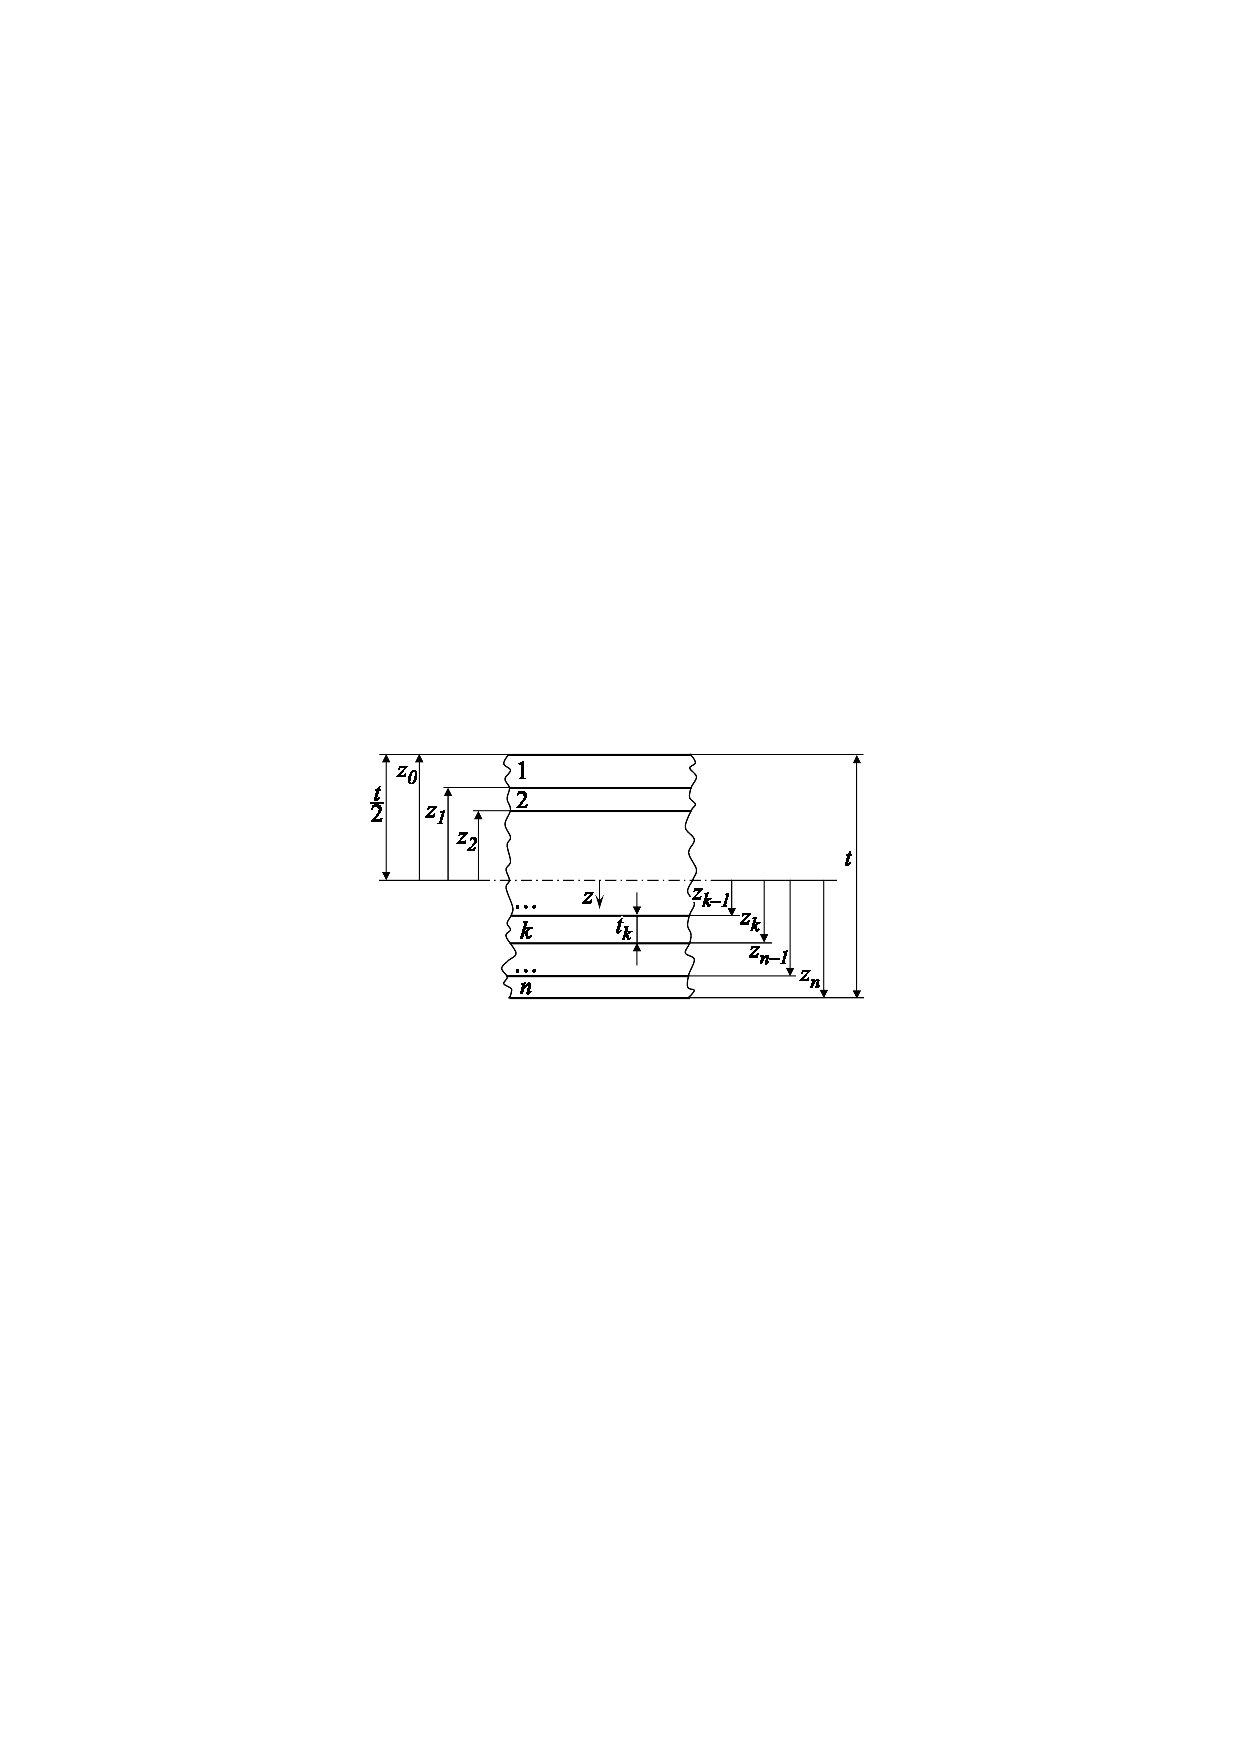
\includegraphics[width=\linewidth]{composite_layers}

    \caption{Иллюстрация модели слоистого композита:}
    \label{fig:sloisty_kompozit}
    $t$ "--- толщина многослойной пластины; \mbox{1, 2, \dots, $k$, \dots, $n$} "--- номер слоя
\end{wrapfigure}

Во второй модели
детали рассматриваем как многослойный композиционный материал
под тепловой нагрузкой.
В качестве координатной плоскости $xy$ принимаем плоскость,
лежащую до~нагружения сборки посередине между её~верхней и~нижней
поверхностями, то есть срединную
плоскость многослойной пластины.
Рисунок~\ref{fig:sloisty_kompozit} иллюстрирует модель слоистого композита.
Положительным направлением оси $z$ считаем направление вниз.

Зависимость для определения
остаточных напряжений в~любой плоскости внутри рассматриваемой сборки
параллельной срединной поверхности
\begin{multline*}
    \boldsymbol{\sigma}
    =
    \mathbf{Q}
    \left(
        \boldsymbol{\epsilon^0}
        +
        z
        \left(
            -
            (\mathbf{D} - \mathbf{B A^{\!\!-1}B})\mathbf{{}^{\!-1}} %притягиваем показатель обратности матрицы
            (\mathbf{B A^{\!\!-1}}) %притягиваем показатель обратности матрицы
            \mathbf{N}^T
            \right.\right. % фейк ради переноса
            + \\ +
            \left. % фейк ради переноса
            (\mathbf{D} - \mathbf{B A^{\!\!-1}B})\mathbf{{}^{\!-1}} %притягиваем показатель обратности матрицы
            \mathbf{M}^T
        \right)
        -
        \int\limits_{T_{b}}^{T_{w}}
        \left. % фейк ради переноса
        \boldsymbol{\alpha}(T)\:\mathrm{d}T
    \right),
\end{multline*}
\noindent где
$\boldsymbol{\sigma}$ "--- вектор напряжений,~Па; %\\
$\mathbf{Q}$ "--- преобразованная матрица жёсткости каждого слоя,~Па;
$\boldsymbol{\epsilon^0}$ "--- относительное удлинение срединной поверхности многослойной композитной пластины (по~осям); %\\
$z$~---~расстояние, измеряемое от~срединной поверхности,~м;
 $ \mathbf{A} $ "--- матрица жёсткости при растяжении (мембранная жёсткость), Н/м;
$ \mathbf{B} $~---~матрица жёсткости изгиб\nb-растяжение (смешанная жёсткость), Н;
$ \mathbf{D} $~---~матрица жёсткости при изгибе (изгибная жёсткость), Н$\cdot$м;
$ \mathbf{N}^T $ "--- усилие, вызванное тепловым воздействием, отнесённое к~единице длины линий, ограничивающих элемент рассматриваемой поверхности, Н/м;
$ \mathbf{M}^T $~---~момент силы, вызванный тепловым воздействием, отнесённый к~единице длины линий, ограничивающих элемент рассматриваемой поверхности, Н;
\(\boldsymbol{\alpha}(T)\) "--- вектор ТКЛР материала, 1/K.

\setlength\intextsep{-0.5ex}%
\begin{wrapfigure}[26]{O}{0.5\textwidth}
    \centering
    \noindent%
    \begingroup%
      \makeatletter%
      \ifx\svgwidth\undefined%
        \setlength{\unitlength}{\linewidth}%
        \ifx\svgscale\undefined%
          \relax%
        \else%
          \setlength{\unitlength}{\unitlength * \real{\svgscale}}%
        \fi%
      \else%
        \setlength{\unitlength}{\svgwidth}%
      \fi%
      \global\let\svgwidth\undefined%
      \global\let\svgscale\undefined%
      \makeatother%
      \begin{picture}(1,0.75870968)%
        \put(0,0){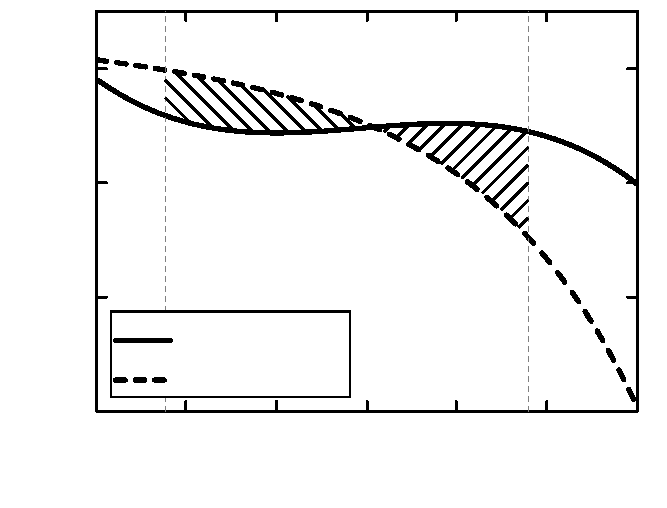
\includegraphics[width=\unitlength]{graphic_integ_lk5_mirror}}%
        \put(0.13379818,0.13843943){\color[named]{black}\makebox(0,0)[rb]{\smash{1}}}%
        \put(0.13198206,0.30434553){\color[named]{black}\makebox(0,0)[rb]{\smash{2}}}%
        \put(0.13243075,0.47250155){\color[named]{black}\makebox(0,0)[rb]{\smash{3}}}%
        \put(0.13125561,0.64322094){\color[named]{black}\makebox(0,0)[rb]{\smash{4}}}%
        \put(0.14691889,0.08513952){\color[named]{black}\makebox(0,0)[b]{\smash{500}}}%
        \put(0.28063032,0.08513952){\color[named]{black}\makebox(0,0)[b]{\smash{400}}}%
        \put(0.41659216,0.08513952){\color[named]{black}\makebox(0,0)[b]{\smash{300}}}%
        \put(0.552554,0.08513952){\color[named]{black}\makebox(0,0)[b]{\smash{200}}}%
        \put(0.68607791,0.08513952){\color[named]{black}\makebox(0,0)[b]{\smash{100}}}%
        \put(0.82078945,0.08513952){\color[named]{black}\makebox(0,0)[b]{\smash{0}}}%
        \put(0.94206112,0.08513952){\color[named]{black}\makebox(0,0)[b]{\smash{$-$100}}}%
        \put(0.06309799,0.44107293){\color[named]{black}\rotatebox{90}{\makebox(0,0)[b]{\smash{ТКЛР, 10\textsuperscript{$-$6}~{\textdegree}C\textsuperscript{$-$1}}}}}%
        \put(0.26708896,0.23391665){\color[named]{black}\makebox(0,0)[lb]{\smash{ЛК5}}}%
        \put(0.26447009,0.17756749){\color[named]{black}\makebox(0,0)[lb]{\smash{Кремний}}}%
        \put(0.79069249,0.685){\color[named]{black}\makebox(0,0)[b]{\smash{20}}}%
        \put(0.24981493,0.685){\color[named]{black}\makebox(0,0)[b]{\smash{422}}}%
      \end{picture}%
    \endgroup%

    \vspace{-2ex}%
    \noindent%
    \begingroup%
      \makeatletter%
      \ifx\svgwidth\undefined%
        \setlength{\unitlength}{\linewidth}%
        \ifx\svgscale\undefined%
          \relax%
        \else%
          \setlength{\unitlength}{\unitlength * \real{\svgscale}}%
        \fi%
      \else%
        \setlength{\unitlength}{\svgwidth}%
      \fi%
      \global\let\svgwidth\undefined%
      \global\let\svgscale\undefined%
      \makeatother%
      \begin{picture}(1,0.77746311)%
        \put(0,0){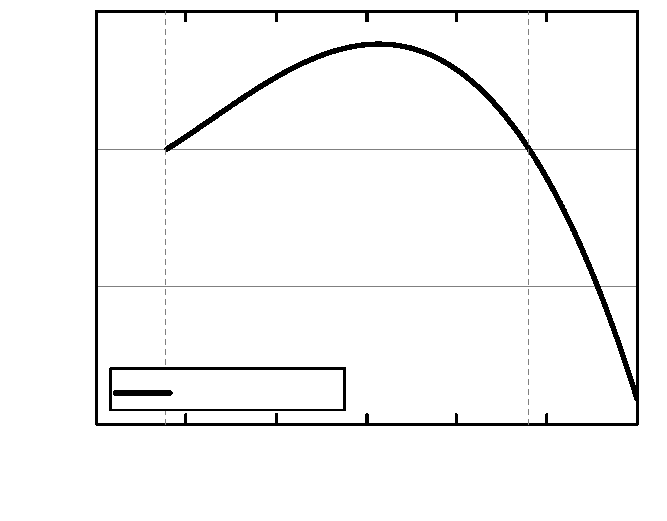
\includegraphics[width=\unitlength]{graphic_integ_lk5_sigma}}%
        \put(0.1330892,0.12928924){\color[named]{black}\makebox(0,0)[rb]{\smash{$-$10}}}%
        \put(0.13274734,0.33651364){\color[named]{black}\makebox(0,0)[rb]{\smash{$-$5}}}%
        \put(0.1330892,0.54117533){\color[named]{black}\makebox(0,0)[rb]{\smash{0}}}%
        \put(0.13274734,0.74564893){\color[named]{black}\makebox(0,0)[rb]{\smash{5}}}%
        \put(0.03769707,0.46873699){\color[named]{black}\rotatebox{90}{\makebox(0,0)[b]{\smash{Напряжения, МПа}}}}%
        \put(0.55242838,0.01292082){\color[named]{black}\makebox(0,0)[b]{\smash{Температура,~{\textdegree}C}}}%
        \put(0.14705445,0.08375692){\color[named]{black}\makebox(0,0)[b]{\smash{500}}}%
        \put(0.28076591,0.08375692){\color[named]{black}\makebox(0,0)[b]{\smash{400}}}%
        \put(0.41672777,0.08375692){\color[named]{black}\makebox(0,0)[b]{\smash{300}}}%
        \put(0.55268964,0.08375692){\color[named]{black}\makebox(0,0)[b]{\smash{200}}}%
        \put(0.68621509,0.08375692){\color[named]{black}\makebox(0,0)[b]{\smash{100}}}%
        \put(0.82092923,0.08375692){\color[named]{black}\makebox(0,0)[b]{\smash{0}}}%
        \put(0.94720432,0.08375692){\color[named]{black}\makebox(0,0)[b]{\smash{$-$100}}}%
        \put(0.2457595,0.69886941){\color[named]{black}\makebox(0,0)[b]{\smash{422}}}%
        \put(0.79085926,0.69886941){\color[named]{black}\makebox(0,0)[b]{\smash{20}}}%
        \put(0.26933091,0.17707933){\color[named]{black}\makebox(0,0)[lb]{\smash{Кремний}}}%
      \end{picture}%
    \endgroup%
    \caption{Формирование остаточных напряжений в процессе охлаждения на~примере соединения стекла ЛК5 с~кремнием}
    \label{graphic_integ}
\end{wrapfigure}

Остаточные напряжения формируются в процессе охлаждения после
завершения процесса анодной посадки.
Рассмотрим на примере
стекла ЛК5 и кремния
(см. Рисунок~\ref{graphic_integ}).

При температуре соединения
в соединённых пластинах не возникает остаточных напряжений
поскольку соединённые кремний и~стекло имеют одинаковую длину.
В процессе охлаждения, пока \mbox{$\alpha_{si} > \alpha_{g}$}
(кремний сжимается быстрее стекла), увеличивается прогиб пластин (вогнутостью
в~сторону пластины кремния).
Также увеличиваются растягивающие напряжения внутри
пластины кремния (при сжимающих напряжениях, их~носитель стремится расшириться,
при растягивающих напряжениях "--- сжаться).
По достижении \mbox{$\alpha_{si} = \alpha_{g}$},
прогиб перестаёт увеличиваться,
достигнув максимального значения.
При продолжении охлаждения кремний сжимается медленнее стекла
\mbox{($\alpha_{si} < \alpha_{g}$)}.
Величина прогиба начинает уменьшаться.
Растягивающие напряжения в~кремнии так же пропорционально снижаются.
При достижении некоторой температуры совокупная накопленная деформация становится
нулевой. Отсутствует прогиб пластин и остаточные напряжения в кремнии и стекле
равны нулю.

Определить температуру проведения процесса электростатического соединения,
обеспечивающую минимальные напряжения при заданной рабочей температуре, можно
графически. Области, отсечённые линиями температур и графиков ТКЛР стекла и
кремния по обе стороны от точки пересечения графиков ТКЛР, должны быть равными
(заштрихованная область на Рисунке~\ref{graphic_integ}).
Для аналитического определения температуры ненапряжённого соединения
интеграл разности температурных зависимостей ТКЛР стекла и кремния от рабочей
температуры до температуры в~момент подачи высокого напряжения должен равняться
нулю.
На~основании измеренных данных
(см. Таблицу~\ref{tab:results_approx_cte})
можно заключить, что
для ЛК5 и рабочей температуры
20~{\textdegree}C температура соединения, обеспечивающая минимальные остаточные
напряжения, составляет 422~{\textdegree}C.

\setlength\intextsep{1ex}%
\begin{figure}[!hb]%Порядок, в котором заданы опции, позволяющие регулировать положение рисунка на странице, не важен — они всегда будут применяться в порядке h (здесь) — t (вверху) — b (внизу) — p (на отдельной странице). Важно только то, какие именно опции заданы. По умолчанию — [tbp]. Задавать опции по одной (например, просто [t] или просто [b]) не рекомендуется — в некоторых случаях это может приводить к проблемным ситуациям.
    \centering
    \ifdefmacro{\tikzsetnextfilename}{\tikzsetnextfilename{syn_a5_nakop_deform}}{}%
    % Created by tikzDevice version 0.10.1 on 2016-07-12 22:00:48
% !TEX encoding = UTF-8 Unicode
\begin{tikzpicture}[x=1pt,y=1pt]
\definecolor{fillColor}{RGB}{255,255,255}
\path[use as bounding box,fill=fillColor] (0,0) rectangle (330.05,214.53);
\begin{scope}
\path[clip] (  0.00,  0.00) rectangle (330.05,214.53);
\definecolor{drawColor}{RGB}{255,255,255}

\path[draw=drawColor,line width= 0.6pt,line join=round,line cap=round,fill=fillColor] (  0.00,  0.00) rectangle (330.05,214.53);
\end{scope}
\begin{scope}
\path[clip] ( 30.99,123.11) rectangle (125.67,201.65);
\definecolor{fillColor}{RGB}{255,255,255}

\path[fill=fillColor] ( 30.99,123.11) rectangle (125.67,201.65);
\definecolor{drawColor}{gray}{0.98}

\path[draw=drawColor,line width= 0.6pt,line join=round] ( 30.99,126.69) --
	(125.67,126.69);

\path[draw=drawColor,line width= 0.6pt,line join=round] ( 30.99,145.95) --
	(125.67,145.95);

\path[draw=drawColor,line width= 0.6pt,line join=round] ( 30.99,165.21) --
	(125.67,165.21);

\path[draw=drawColor,line width= 0.6pt,line join=round] ( 30.99,184.48) --
	(125.67,184.48);

\path[draw=drawColor,line width= 0.6pt,line join=round] ( 53.10,123.11) --
	( 53.10,201.65);

\path[draw=drawColor,line width= 0.6pt,line join=round] ( 76.85,123.11) --
	( 76.85,201.65);

\path[draw=drawColor,line width= 0.6pt,line join=round] ( 94.65,123.11) --
	( 94.65,201.65);

\path[draw=drawColor,line width= 0.6pt,line join=round] (113.95,123.11) --
	(113.95,201.65);
\definecolor{drawColor}{gray}{0.80}

\path[draw=drawColor,line width= 0.4pt,line join=round] ( 30.99,136.32) --
	(125.67,136.32);

\path[draw=drawColor,line width= 0.4pt,line join=round] ( 30.99,155.58) --
	(125.67,155.58);

\path[draw=drawColor,line width= 0.4pt,line join=round] ( 30.99,174.85) --
	(125.67,174.85);

\path[draw=drawColor,line width= 0.4pt,line join=round] ( 30.99,194.11) --
	(125.67,194.11);

\path[draw=drawColor,line width= 0.4pt,line join=round] ( 35.29,123.11) --
	( 35.29,201.65);

\path[draw=drawColor,line width= 0.4pt,line join=round] ( 70.91,123.11) --
	( 70.91,201.65);

\path[draw=drawColor,line width= 0.4pt,line join=round] ( 82.78,123.11) --
	( 82.78,201.65);

\path[draw=drawColor,line width= 0.4pt,line join=round] (106.53,123.11) --
	(106.53,201.65);

\path[draw=drawColor,line width= 0.4pt,line join=round] (121.37,123.11) --
	(121.37,201.65);
\definecolor{drawColor}{RGB}{0,0,0}

\path[draw=drawColor,line width= 1.4pt,line join=round] ( 35.29,132.40) --
	( 35.59,132.58) --
	( 35.88,132.76) --
	( 36.18,132.94) --
	( 36.48,133.12) --
	( 36.78,133.29) --
	( 37.07,133.47) --
	( 37.37,133.65) --
	( 37.67,133.82) --
	( 37.96,134.00) --
	( 38.26,134.17) --
	( 38.56,134.34) --
	( 38.85,134.52) --
	( 39.15,134.69) --
	( 39.45,134.86) --
	( 39.74,135.03) --
	( 40.04,135.20) --
	( 40.34,135.37) --
	( 40.63,135.54) --
	( 40.93,135.71) --
	( 41.23,135.88) --
	( 41.52,136.05) --
	( 41.82,136.21) --
	( 42.12,136.38) --
	( 42.41,136.54) --
	( 42.71,136.71) --
	( 43.01,136.87) --
	( 43.31,137.04) --
	( 43.60,137.20) --
	( 43.90,137.36) --
	( 44.20,137.53) --
	( 44.49,137.69) --
	( 44.79,137.85) --
	( 45.09,138.01) --
	( 45.38,138.17) --
	( 45.68,138.33) --
	( 45.98,138.49) --
	( 46.27,138.65) --
	( 46.57,138.80) --
	( 46.87,138.96) --
	( 47.16,139.12) --
	( 47.46,139.27) --
	( 47.76,139.43) --
	( 48.05,139.58) --
	( 48.35,139.74) --
	( 48.65,139.89) --
	( 48.94,140.04) --
	( 49.24,140.20) --
	( 49.54,140.35) --
	( 49.84,140.50) --
	( 50.13,140.65) --
	( 50.43,140.80) --
	( 50.73,140.95) --
	( 51.02,141.10) --
	( 51.32,141.25) --
	( 51.62,141.39) --
	( 51.91,141.54) --
	( 52.21,141.69) --
	( 52.51,141.84) --
	( 52.80,141.98) --
	( 53.10,142.13) --
	( 53.40,142.27) --
	( 53.69,142.42) --
	( 53.99,142.56) --
	( 54.29,142.70) --
	( 54.58,142.84) --
	( 54.88,142.99) --
	( 55.18,143.13) --
	( 55.47,143.27) --
	( 55.77,143.41) --
	( 56.07,143.55) --
	( 56.36,143.69) --
	( 56.66,143.83) --
	( 56.96,143.97) --
	( 57.26,144.10) --
	( 57.55,144.24) --
	( 57.85,144.38) --
	( 58.15,144.51) --
	( 58.44,144.65) --
	( 58.74,144.78) --
	( 59.04,144.92) --
	( 59.33,145.05) --
	( 59.63,145.19) --
	( 59.93,145.32) --
	( 60.22,145.45) --
	( 60.52,145.58) --
	( 60.82,145.71) --
	( 61.11,145.84) --
	( 61.41,145.97) --
	( 61.71,146.10) --
	( 62.00,146.23) --
	( 62.30,146.36) --
	( 62.60,146.49) --
	( 62.89,146.62) --
	( 63.19,146.75) --
	( 63.49,146.87) --
	( 63.79,147.00) --
	( 64.08,147.12) --
	( 64.38,147.25) --
	( 64.68,147.37) --
	( 64.97,147.50) --
	( 65.27,147.62) --
	( 65.57,147.75) --
	( 65.86,147.87) --
	( 66.16,147.99) --
	( 66.46,148.11) --
	( 66.75,148.23) --
	( 67.05,148.35) --
	( 67.35,148.47) --
	( 67.64,148.59) --
	( 67.94,148.71) --
	( 68.24,148.83) --
	( 68.53,148.95) --
	( 68.83,149.07) --
	( 69.13,149.18) --
	( 69.42,149.30) --
	( 69.72,149.42) --
	( 70.02,149.53) --
	( 70.32,149.65) --
	( 70.61,149.76) --
	( 70.91,149.88) --
	( 71.21,149.99) --
	( 71.50,150.10) --
	( 71.80,150.22) --
	( 72.10,150.33) --
	( 72.39,150.44) --
	( 72.69,150.55) --
	( 72.99,150.66) --
	( 73.28,150.77) --
	( 73.58,150.88) --
	( 73.88,150.99) --
	( 74.17,151.10) --
	( 74.47,151.21) --
	( 74.77,151.32) --
	( 75.06,151.43) --
	( 75.36,151.53) --
	( 75.66,151.64) --
	( 75.95,151.75) --
	( 76.25,151.85) --
	( 76.55,151.96) --
	( 76.85,152.06) --
	( 77.14,152.17) --
	( 77.44,152.27) --
	( 77.74,152.37) --
	( 78.03,152.48) --
	( 78.33,152.58) --
	( 78.63,152.68) --
	( 78.92,152.78) --
	( 79.22,152.88) --
	( 79.52,152.98) --
	( 79.81,153.08) --
	( 80.11,153.18) --
	( 80.41,153.28) --
	( 80.70,153.38) --
	( 81.00,153.48) --
	( 81.30,153.58) --
	( 81.59,153.67) --
	( 81.89,153.77) --
	( 82.19,153.87) --
	( 82.48,153.96) --
	( 82.78,154.06) --
	( 83.08,154.15) --
	( 83.38,154.25) --
	( 83.67,154.34) --
	( 83.97,154.44) --
	( 84.27,154.53) --
	( 84.56,154.62) --
	( 84.86,154.71) --
	( 85.16,154.81) --
	( 85.45,154.90) --
	( 85.75,154.99) --
	( 86.05,155.08) --
	( 86.34,155.17) --
	( 86.64,155.26) --
	( 86.94,155.35) --
	( 87.23,155.44) --
	( 87.53,155.52) --
	( 87.83,155.61) --
	( 88.12,155.70) --
	( 88.42,155.79) --
	( 88.72,155.87) --
	( 89.01,155.96) --
	( 89.31,156.05) --
	( 89.61,156.13) --
	( 89.91,156.22) --
	( 90.20,156.30) --
	( 90.50,156.38) --
	( 90.80,156.47) --
	( 91.09,156.55) --
	( 91.39,156.63) --
	( 91.69,156.72) --
	( 91.98,156.80) --
	( 92.28,156.88) --
	( 92.58,156.96) --
	( 92.87,157.04) --
	( 93.17,157.12) --
	( 93.47,157.20) --
	( 93.76,157.28) --
	( 94.06,157.36) --
	( 94.36,157.44) --
	( 94.65,157.52) --
	( 94.95,157.59) --
	( 95.25,157.67) --
	( 95.54,157.75) --
	( 95.84,157.83) --
	( 96.14,157.90) --
	( 96.44,157.98) --
	( 96.73,158.05) --
	( 97.03,158.13) --
	( 97.33,158.20) --
	( 97.62,158.28) --
	( 97.92,158.35) --
	( 98.22,158.42) --
	( 98.51,158.50) --
	( 98.81,158.57) --
	( 99.11,158.64) --
	( 99.40,158.71) --
	( 99.70,158.78) --
	(100.00,158.85) --
	(100.29,158.92) --
	(100.59,158.99) --
	(100.89,159.06) --
	(101.18,159.13) --
	(101.48,159.20) --
	(101.78,159.27) --
	(102.07,159.34) --
	(102.37,159.40) --
	(102.67,159.47) --
	(102.97,159.54) --
	(103.26,159.60) --
	(103.56,159.67) --
	(103.86,159.74) --
	(104.15,159.80) --
	(104.45,159.87) --
	(104.75,159.93) --
	(105.04,159.99) --
	(105.34,160.06) --
	(105.64,160.12) --
	(105.93,160.18) --
	(106.23,160.25) --
	(106.53,160.31) --
	(106.82,160.37) --
	(107.12,160.43) --
	(107.42,160.49) --
	(107.71,160.55) --
	(108.01,160.61) --
	(108.31,160.67) --
	(108.60,160.73) --
	(108.90,160.79) --
	(109.20,160.85) --
	(109.50,160.91) --
	(109.79,160.97) --
	(110.09,161.02) --
	(110.39,161.08) --
	(110.68,161.14) --
	(110.98,161.19) --
	(111.28,161.25) --
	(111.57,161.30) --
	(111.87,161.36) --
	(112.17,161.41) --
	(112.46,161.47) --
	(112.76,161.52) --
	(113.06,161.58) --
	(113.35,161.63) --
	(113.65,161.68) --
	(113.95,161.74) --
	(114.24,161.79) --
	(114.54,161.84) --
	(114.84,161.89) --
	(115.13,161.94) --
	(115.43,161.99) --
	(115.73,162.04) --
	(116.03,162.09) --
	(116.32,162.14) --
	(116.62,162.19) --
	(116.92,162.24) --
	(117.21,162.29) --
	(117.51,162.34) --
	(117.81,162.39) --
	(118.10,162.43) --
	(118.40,162.48) --
	(118.70,162.53) --
	(118.99,162.57) --
	(119.29,162.62) --
	(119.59,162.67) --
	(119.88,162.71) --
	(120.18,162.76) --
	(120.48,162.80) --
	(120.77,162.84) --
	(121.07,162.89) --
	(121.37,162.93);

\path[draw=drawColor,line width= 1.4pt,dash pattern=on 7pt off 3pt ,line join=round] ( 35.29,144.09) --
	( 35.59,144.27) --
	( 35.88,144.45) --
	( 36.18,144.63) --
	( 36.48,144.81) --
	( 36.78,144.99) --
	( 37.07,145.16) --
	( 37.37,145.34) --
	( 37.67,145.51) --
	( 37.96,145.69) --
	( 38.26,145.86) --
	( 38.56,146.03) --
	( 38.85,146.21) --
	( 39.15,146.38) --
	( 39.45,146.55) --
	( 39.74,146.72) --
	( 40.04,146.89) --
	( 40.34,147.06) --
	( 40.63,147.23) --
	( 40.93,147.40) --
	( 41.23,147.57) --
	( 41.52,147.74) --
	( 41.82,147.90) --
	( 42.12,148.07) --
	( 42.41,148.23) --
	( 42.71,148.40) --
	( 43.01,148.56) --
	( 43.31,148.73) --
	( 43.60,148.89) --
	( 43.90,149.05) --
	( 44.20,149.22) --
	( 44.49,149.38) --
	( 44.79,149.54) --
	( 45.09,149.70) --
	( 45.38,149.86) --
	( 45.68,150.02) --
	( 45.98,150.18) --
	( 46.27,150.34) --
	( 46.57,150.49) --
	( 46.87,150.65) --
	( 47.16,150.81) --
	( 47.46,150.96) --
	( 47.76,151.12) --
	( 48.05,151.27) --
	( 48.35,151.43) --
	( 48.65,151.58) --
	( 48.94,151.73) --
	( 49.24,151.89) --
	( 49.54,152.04) --
	( 49.84,152.19) --
	( 50.13,152.34) --
	( 50.43,152.49) --
	( 50.73,152.64) --
	( 51.02,152.79) --
	( 51.32,152.94) --
	( 51.62,153.09) --
	( 51.91,153.23) --
	( 52.21,153.38) --
	( 52.51,153.53) --
	( 52.80,153.67) --
	( 53.10,153.82) --
	( 53.40,153.96) --
	( 53.69,154.11) --
	( 53.99,154.25) --
	( 54.29,154.39) --
	( 54.58,154.53) --
	( 54.88,154.68) --
	( 55.18,154.82) --
	( 55.47,154.96) --
	( 55.77,155.10) --
	( 56.07,155.24) --
	( 56.36,155.38) --
	( 56.66,155.52) --
	( 56.96,155.66) --
	( 57.26,155.79) --
	( 57.55,155.93) --
	( 57.85,156.07) --
	( 58.15,156.20) --
	( 58.44,156.34) --
	( 58.74,156.47) --
	( 59.04,156.61) --
	( 59.33,156.74) --
	( 59.63,156.88) --
	( 59.93,157.01) --
	( 60.22,157.14) --
	( 60.52,157.27) --
	( 60.82,157.40) --
	( 61.11,157.54) --
	( 61.41,157.67) --
	( 61.71,157.80) --
	( 62.00,157.92) --
	( 62.30,158.05) --
	( 62.60,158.18) --
	( 62.89,158.31) --
	( 63.19,158.44) --
	( 63.49,158.56) --
	( 63.79,158.69) --
	( 64.08,158.82) --
	( 64.38,158.94) --
	( 64.68,159.06) --
	( 64.97,159.19) --
	( 65.27,159.31) --
	( 65.57,159.44) --
	( 65.86,159.56) --
	( 66.16,159.68) --
	( 66.46,159.80) --
	( 66.75,159.92) --
	( 67.05,160.04) --
	( 67.35,160.16) --
	( 67.64,160.28) --
	( 67.94,160.40) --
	( 68.24,160.52) --
	( 68.53,160.64) --
	( 68.83,160.76) --
	( 69.13,160.87) --
	( 69.42,160.99) --
	( 69.72,161.11) --
	( 70.02,161.22) --
	( 70.32,161.34) --
	( 70.61,161.45) --
	( 70.91,161.57) --
	( 71.21,161.68) --
	( 71.50,161.79) --
	( 71.80,161.91) --
	( 72.10,162.02) --
	( 72.39,162.13) --
	( 72.69,162.24) --
	( 72.99,162.35) --
	( 73.28,162.46) --
	( 73.58,162.57) --
	( 73.88,162.68) --
	( 74.17,162.79) --
	( 74.47,162.90) --
	( 74.77,163.01) --
	( 75.06,163.12) --
	( 75.36,163.22) --
	( 75.66,163.33) --
	( 75.95,163.44) --
	( 76.25,163.54) --
	( 76.55,163.65) --
	( 76.85,163.75) --
	( 77.14,163.86) --
	( 77.44,163.96) --
	( 77.74,164.06) --
	( 78.03,164.17) --
	( 78.33,164.27) --
	( 78.63,164.37) --
	( 78.92,164.47) --
	( 79.22,164.57) --
	( 79.52,164.67) --
	( 79.81,164.77) --
	( 80.11,164.87) --
	( 80.41,164.97) --
	( 80.70,165.07) --
	( 81.00,165.17) --
	( 81.30,165.27) --
	( 81.59,165.36) --
	( 81.89,165.46) --
	( 82.19,165.56) --
	( 82.48,165.65) --
	( 82.78,165.75) --
	( 83.08,165.84) --
	( 83.38,165.94) --
	( 83.67,166.03) --
	( 83.97,166.13) --
	( 84.27,166.22) --
	( 84.56,166.31) --
	( 84.86,166.40) --
	( 85.16,166.50) --
	( 85.45,166.59) --
	( 85.75,166.68) --
	( 86.05,166.77) --
	( 86.34,166.86) --
	( 86.64,166.95) --
	( 86.94,167.04) --
	( 87.23,167.13) --
	( 87.53,167.22) --
	( 87.83,167.30) --
	( 88.12,167.39) --
	( 88.42,167.48) --
	( 88.72,167.56) --
	( 89.01,167.65) --
	( 89.31,167.74) --
	( 89.61,167.82) --
	( 89.91,167.91) --
	( 90.20,167.99) --
	( 90.50,168.08) --
	( 90.80,168.16) --
	( 91.09,168.24) --
	( 91.39,168.32) --
	( 91.69,168.41) --
	( 91.98,168.49) --
	( 92.28,168.57) --
	( 92.58,168.65) --
	( 92.87,168.73) --
	( 93.17,168.81) --
	( 93.47,168.89) --
	( 93.76,168.97) --
	( 94.06,169.05) --
	( 94.36,169.13) --
	( 94.65,169.21) --
	( 94.95,169.29) --
	( 95.25,169.36) --
	( 95.54,169.44) --
	( 95.84,169.52) --
	( 96.14,169.59) --
	( 96.44,169.67) --
	( 96.73,169.74) --
	( 97.03,169.82) --
	( 97.33,169.89) --
	( 97.62,169.97) --
	( 97.92,170.04) --
	( 98.22,170.11) --
	( 98.51,170.19) --
	( 98.81,170.26) --
	( 99.11,170.33) --
	( 99.40,170.40) --
	( 99.70,170.47) --
	(100.00,170.54) --
	(100.29,170.61) --
	(100.59,170.68) --
	(100.89,170.75) --
	(101.18,170.82) --
	(101.48,170.89) --
	(101.78,170.96) --
	(102.07,171.03) --
	(102.37,171.09) --
	(102.67,171.16) --
	(102.97,171.23) --
	(103.26,171.30) --
	(103.56,171.36) --
	(103.86,171.43) --
	(104.15,171.49) --
	(104.45,171.56) --
	(104.75,171.62) --
	(105.04,171.68) --
	(105.34,171.75) --
	(105.64,171.81) --
	(105.93,171.87) --
	(106.23,171.94) --
	(106.53,172.00) --
	(106.82,172.06) --
	(107.12,172.12) --
	(107.42,172.18) --
	(107.71,172.24) --
	(108.01,172.30) --
	(108.31,172.36) --
	(108.60,172.42) --
	(108.90,172.48) --
	(109.20,172.54) --
	(109.50,172.60) --
	(109.79,172.66) --
	(110.09,172.71) --
	(110.39,172.77) --
	(110.68,172.83) --
	(110.98,172.88) --
	(111.28,172.94) --
	(111.57,172.99) --
	(111.87,173.05) --
	(112.17,173.10) --
	(112.46,173.16) --
	(112.76,173.21) --
	(113.06,173.27) --
	(113.35,173.32) --
	(113.65,173.37) --
	(113.95,173.43) --
	(114.24,173.48) --
	(114.54,173.53) --
	(114.84,173.58) --
	(115.13,173.63) --
	(115.43,173.68) --
	(115.73,173.73) --
	(116.03,173.78) --
	(116.32,173.83) --
	(116.62,173.88) --
	(116.92,173.93) --
	(117.21,173.98) --
	(117.51,174.03) --
	(117.81,174.08) --
	(118.10,174.12) --
	(118.40,174.17) --
	(118.70,174.22) --
	(118.99,174.26) --
	(119.29,174.31) --
	(119.59,174.36) --
	(119.88,174.40) --
	(120.18,174.45) --
	(120.48,174.49) --
	(120.77,174.53) --
	(121.07,174.58) --
	(121.37,174.62);

\path[draw=drawColor,line width= 1.4pt,dash pattern=on 1pt off 3pt ,line join=round] ( 35.29,159.04) --
	( 35.59,159.22) --
	( 35.88,159.39) --
	( 36.18,159.57) --
	( 36.48,159.75) --
	( 36.78,159.93) --
	( 37.07,160.10) --
	( 37.37,160.28) --
	( 37.67,160.46) --
	( 37.96,160.63) --
	( 38.26,160.80) --
	( 38.56,160.98) --
	( 38.85,161.15) --
	( 39.15,161.32) --
	( 39.45,161.49) --
	( 39.74,161.67) --
	( 40.04,161.84) --
	( 40.34,162.01) --
	( 40.63,162.17) --
	( 40.93,162.34) --
	( 41.23,162.51) --
	( 41.52,162.68) --
	( 41.82,162.85) --
	( 42.12,163.01) --
	( 42.41,163.18) --
	( 42.71,163.34) --
	( 43.01,163.51) --
	( 43.31,163.67) --
	( 43.60,163.83) --
	( 43.90,164.00) --
	( 44.20,164.16) --
	( 44.49,164.32) --
	( 44.79,164.48) --
	( 45.09,164.64) --
	( 45.38,164.80) --
	( 45.68,164.96) --
	( 45.98,165.12) --
	( 46.27,165.28) --
	( 46.57,165.44) --
	( 46.87,165.59) --
	( 47.16,165.75) --
	( 47.46,165.91) --
	( 47.76,166.06) --
	( 48.05,166.22) --
	( 48.35,166.37) --
	( 48.65,166.52) --
	( 48.94,166.68) --
	( 49.24,166.83) --
	( 49.54,166.98) --
	( 49.84,167.13) --
	( 50.13,167.28) --
	( 50.43,167.43) --
	( 50.73,167.58) --
	( 51.02,167.73) --
	( 51.32,167.88) --
	( 51.62,168.03) --
	( 51.91,168.18) --
	( 52.21,168.32) --
	( 52.51,168.47) --
	( 52.80,168.61) --
	( 53.10,168.76) --
	( 53.40,168.90) --
	( 53.69,169.05) --
	( 53.99,169.19) --
	( 54.29,169.34) --
	( 54.58,169.48) --
	( 54.88,169.62) --
	( 55.18,169.76) --
	( 55.47,169.90) --
	( 55.77,170.04) --
	( 56.07,170.18) --
	( 56.36,170.32) --
	( 56.66,170.46) --
	( 56.96,170.60) --
	( 57.26,170.74) --
	( 57.55,170.87) --
	( 57.85,171.01) --
	( 58.15,171.15) --
	( 58.44,171.28) --
	( 58.74,171.42) --
	( 59.04,171.55) --
	( 59.33,171.69) --
	( 59.63,171.82) --
	( 59.93,171.95) --
	( 60.22,172.08) --
	( 60.52,172.22) --
	( 60.82,172.35) --
	( 61.11,172.48) --
	( 61.41,172.61) --
	( 61.71,172.74) --
	( 62.00,172.87) --
	( 62.30,173.00) --
	( 62.60,173.12) --
	( 62.89,173.25) --
	( 63.19,173.38) --
	( 63.49,173.51) --
	( 63.79,173.63) --
	( 64.08,173.76) --
	( 64.38,173.88) --
	( 64.68,174.01) --
	( 64.97,174.13) --
	( 65.27,174.26) --
	( 65.57,174.38) --
	( 65.86,174.50) --
	( 66.16,174.62) --
	( 66.46,174.75) --
	( 66.75,174.87) --
	( 67.05,174.99) --
	( 67.35,175.11) --
	( 67.64,175.23) --
	( 67.94,175.35) --
	( 68.24,175.46) --
	( 68.53,175.58) --
	( 68.83,175.70) --
	( 69.13,175.82) --
	( 69.42,175.93) --
	( 69.72,176.05) --
	( 70.02,176.17) --
	( 70.32,176.28) --
	( 70.61,176.40) --
	( 70.91,176.51) --
	( 71.21,176.62) --
	( 71.50,176.74) --
	( 71.80,176.85) --
	( 72.10,176.96) --
	( 72.39,177.07) --
	( 72.69,177.19) --
	( 72.99,177.30) --
	( 73.28,177.41) --
	( 73.58,177.52) --
	( 73.88,177.63) --
	( 74.17,177.74) --
	( 74.47,177.84) --
	( 74.77,177.95) --
	( 75.06,178.06) --
	( 75.36,178.17) --
	( 75.66,178.27) --
	( 75.95,178.38) --
	( 76.25,178.48) --
	( 76.55,178.59) --
	( 76.85,178.69) --
	( 77.14,178.80) --
	( 77.44,178.90) --
	( 77.74,179.01) --
	( 78.03,179.11) --
	( 78.33,179.21) --
	( 78.63,179.31) --
	( 78.92,179.41) --
	( 79.22,179.51) --
	( 79.52,179.62) --
	( 79.81,179.72) --
	( 80.11,179.82) --
	( 80.41,179.91) --
	( 80.70,180.01) --
	( 81.00,180.11) --
	( 81.30,180.21) --
	( 81.59,180.31) --
	( 81.89,180.40) --
	( 82.19,180.50) --
	( 82.48,180.60) --
	( 82.78,180.69) --
	( 83.08,180.79) --
	( 83.38,180.88) --
	( 83.67,180.97) --
	( 83.97,181.07) --
	( 84.27,181.16) --
	( 84.56,181.25) --
	( 84.86,181.35) --
	( 85.16,181.44) --
	( 85.45,181.53) --
	( 85.75,181.62) --
	( 86.05,181.71) --
	( 86.34,181.80) --
	( 86.64,181.89) --
	( 86.94,181.98) --
	( 87.23,182.07) --
	( 87.53,182.16) --
	( 87.83,182.25) --
	( 88.12,182.33) --
	( 88.42,182.42) --
	( 88.72,182.51) --
	( 89.01,182.59) --
	( 89.31,182.68) --
	( 89.61,182.76) --
	( 89.91,182.85) --
	( 90.20,182.93) --
	( 90.50,183.02) --
	( 90.80,183.10) --
	( 91.09,183.18) --
	( 91.39,183.27) --
	( 91.69,183.35) --
	( 91.98,183.43) --
	( 92.28,183.51) --
	( 92.58,183.59) --
	( 92.87,183.68) --
	( 93.17,183.76) --
	( 93.47,183.84) --
	( 93.76,183.91) --
	( 94.06,183.99) --
	( 94.36,184.07) --
	( 94.65,184.15) --
	( 94.95,184.23) --
	( 95.25,184.31) --
	( 95.54,184.38) --
	( 95.84,184.46) --
	( 96.14,184.53) --
	( 96.44,184.61) --
	( 96.73,184.69) --
	( 97.03,184.76) --
	( 97.33,184.83) --
	( 97.62,184.91) --
	( 97.92,184.98) --
	( 98.22,185.06) --
	( 98.51,185.13) --
	( 98.81,185.20) --
	( 99.11,185.27) --
	( 99.40,185.34) --
	( 99.70,185.42) --
	(100.00,185.49) --
	(100.29,185.56) --
	(100.59,185.63) --
	(100.89,185.70) --
	(101.18,185.77) --
	(101.48,185.83) --
	(101.78,185.90) --
	(102.07,185.97) --
	(102.37,186.04) --
	(102.67,186.10) --
	(102.97,186.17) --
	(103.26,186.24) --
	(103.56,186.30) --
	(103.86,186.37) --
	(104.15,186.43) --
	(104.45,186.50) --
	(104.75,186.56) --
	(105.04,186.63) --
	(105.34,186.69) --
	(105.64,186.75) --
	(105.93,186.82) --
	(106.23,186.88) --
	(106.53,186.94) --
	(106.82,187.00) --
	(107.12,187.06) --
	(107.42,187.13) --
	(107.71,187.19) --
	(108.01,187.25) --
	(108.31,187.31) --
	(108.60,187.37) --
	(108.90,187.42) --
	(109.20,187.48) --
	(109.50,187.54) --
	(109.79,187.60) --
	(110.09,187.66) --
	(110.39,187.71) --
	(110.68,187.77) --
	(110.98,187.83) --
	(111.28,187.88) --
	(111.57,187.94) --
	(111.87,187.99) --
	(112.17,188.05) --
	(112.46,188.10) --
	(112.76,188.16) --
	(113.06,188.21) --
	(113.35,188.26) --
	(113.65,188.32) --
	(113.95,188.37) --
	(114.24,188.42) --
	(114.54,188.47) --
	(114.84,188.52) --
	(115.13,188.58) --
	(115.43,188.63) --
	(115.73,188.68) --
	(116.03,188.73) --
	(116.32,188.78) --
	(116.62,188.83) --
	(116.92,188.87) --
	(117.21,188.92) --
	(117.51,188.97) --
	(117.81,189.02) --
	(118.10,189.07) --
	(118.40,189.11) --
	(118.70,189.16) --
	(118.99,189.21) --
	(119.29,189.25) --
	(119.59,189.30) --
	(119.88,189.34) --
	(120.18,189.39) --
	(120.48,189.43) --
	(120.77,189.48) --
	(121.07,189.52) --
	(121.37,189.56);

\path[draw=drawColor,line width= 0.9pt,line join=round,line cap=round] ( 30.99,123.11) rectangle (125.67,201.65);
\end{scope}
\begin{scope}
\path[clip] (131.67,123.11) rectangle (226.36,201.65);
\definecolor{fillColor}{RGB}{255,255,255}

\path[fill=fillColor] (131.67,123.11) rectangle (226.36,201.65);
\definecolor{drawColor}{gray}{0.98}

\path[draw=drawColor,line width= 0.6pt,line join=round] (131.67,126.69) --
	(226.36,126.69);

\path[draw=drawColor,line width= 0.6pt,line join=round] (131.67,145.95) --
	(226.36,145.95);

\path[draw=drawColor,line width= 0.6pt,line join=round] (131.67,165.21) --
	(226.36,165.21);

\path[draw=drawColor,line width= 0.6pt,line join=round] (131.67,184.48) --
	(226.36,184.48);

\path[draw=drawColor,line width= 0.6pt,line join=round] (153.78,123.11) --
	(153.78,201.65);

\path[draw=drawColor,line width= 0.6pt,line join=round] (177.53,123.11) --
	(177.53,201.65);

\path[draw=drawColor,line width= 0.6pt,line join=round] (195.34,123.11) --
	(195.34,201.65);

\path[draw=drawColor,line width= 0.6pt,line join=round] (214.63,123.11) --
	(214.63,201.65);
\definecolor{drawColor}{gray}{0.80}

\path[draw=drawColor,line width= 0.4pt,line join=round] (131.67,136.32) --
	(226.36,136.32);

\path[draw=drawColor,line width= 0.4pt,line join=round] (131.67,155.58) --
	(226.36,155.58);

\path[draw=drawColor,line width= 0.4pt,line join=round] (131.67,174.85) --
	(226.36,174.85);

\path[draw=drawColor,line width= 0.4pt,line join=round] (131.67,194.11) --
	(226.36,194.11);

\path[draw=drawColor,line width= 0.4pt,line join=round] (135.98,123.11) --
	(135.98,201.65);

\path[draw=drawColor,line width= 0.4pt,line join=round] (171.59,123.11) --
	(171.59,201.65);

\path[draw=drawColor,line width= 0.4pt,line join=round] (183.47,123.11) --
	(183.47,201.65);

\path[draw=drawColor,line width= 0.4pt,line join=round] (207.21,123.11) --
	(207.21,201.65);

\path[draw=drawColor,line width= 0.4pt,line join=round] (222.05,123.11) --
	(222.05,201.65);
\definecolor{drawColor}{RGB}{0,0,0}

\path[draw=drawColor,line width= 1.4pt,line join=round] (135.98,126.68) --
	(136.27,126.83) --
	(136.57,126.99) --
	(136.87,127.14) --
	(137.16,127.29) --
	(137.46,127.44) --
	(137.76,127.59) --
	(138.05,127.74) --
	(138.35,127.89) --
	(138.65,128.04) --
	(138.94,128.19) --
	(139.24,128.34) --
	(139.54,128.49) --
	(139.83,128.64) --
	(140.13,128.78) --
	(140.43,128.93) --
	(140.72,129.08) --
	(141.02,129.22) --
	(141.32,129.37) --
	(141.62,129.51) --
	(141.91,129.66) --
	(142.21,129.80) --
	(142.51,129.95) --
	(142.80,130.09) --
	(143.10,130.23) --
	(143.40,130.38) --
	(143.69,130.52) --
	(143.99,130.66) --
	(144.29,130.80) --
	(144.58,130.94) --
	(144.88,131.09) --
	(145.18,131.23) --
	(145.47,131.37) --
	(145.77,131.50) --
	(146.07,131.64) --
	(146.36,131.78) --
	(146.66,131.92) --
	(146.96,132.06) --
	(147.25,132.20) --
	(147.55,132.33) --
	(147.85,132.47) --
	(148.14,132.61) --
	(148.44,132.74) --
	(148.74,132.88) --
	(149.04,133.01) --
	(149.33,133.15) --
	(149.63,133.28) --
	(149.93,133.41) --
	(150.22,133.55) --
	(150.52,133.68) --
	(150.82,133.81) --
	(151.11,133.94) --
	(151.41,134.08) --
	(151.71,134.21) --
	(152.00,134.34) --
	(152.30,134.47) --
	(152.60,134.60) --
	(152.89,134.73) --
	(153.19,134.86) --
	(153.49,134.99) --
	(153.78,135.11) --
	(154.08,135.24) --
	(154.38,135.37) --
	(154.67,135.50) --
	(154.97,135.62) --
	(155.27,135.75) --
	(155.57,135.88) --
	(155.86,136.00) --
	(156.16,136.13) --
	(156.46,136.25) --
	(156.75,136.38) --
	(157.05,136.50) --
	(157.35,136.63) --
	(157.64,136.75) --
	(157.94,136.87) --
	(158.24,136.99) --
	(158.53,137.12) --
	(158.83,137.24) --
	(159.13,137.36) --
	(159.42,137.48) --
	(159.72,137.60) --
	(160.02,137.72) --
	(160.31,137.84) --
	(160.61,137.96) --
	(160.91,138.08) --
	(161.20,138.20) --
	(161.50,138.32) --
	(161.80,138.43) --
	(162.10,138.55) --
	(162.39,138.67) --
	(162.69,138.78) --
	(162.99,138.90) --
	(163.28,139.02) --
	(163.58,139.13) --
	(163.88,139.25) --
	(164.17,139.36) --
	(164.47,139.48) --
	(164.77,139.59) --
	(165.06,139.70) --
	(165.36,139.82) --
	(165.66,139.93) --
	(165.95,140.04) --
	(166.25,140.16) --
	(166.55,140.27) --
	(166.84,140.38) --
	(167.14,140.49) --
	(167.44,140.60) --
	(167.73,140.71) --
	(168.03,140.82) --
	(168.33,140.93) --
	(168.63,141.04) --
	(168.92,141.15) --
	(169.22,141.26) --
	(169.52,141.36) --
	(169.81,141.47) --
	(170.11,141.58) --
	(170.41,141.69) --
	(170.70,141.79) --
	(171.00,141.90) --
	(171.30,142.00) --
	(171.59,142.11) --
	(171.89,142.21) --
	(172.19,142.32) --
	(172.48,142.42) --
	(172.78,142.53) --
	(173.08,142.63) --
	(173.37,142.73) --
	(173.67,142.84) --
	(173.97,142.94) --
	(174.26,143.04) --
	(174.56,143.14) --
	(174.86,143.25) --
	(175.16,143.35) --
	(175.45,143.45) --
	(175.75,143.55) --
	(176.05,143.65) --
	(176.34,143.75) --
	(176.64,143.85) --
	(176.94,143.95) --
	(177.23,144.04) --
	(177.53,144.14) --
	(177.83,144.24) --
	(178.12,144.34) --
	(178.42,144.43) --
	(178.72,144.53) --
	(179.01,144.63) --
	(179.31,144.72) --
	(179.61,144.82) --
	(179.90,144.91) --
	(180.20,145.01) --
	(180.50,145.10) --
	(180.79,145.20) --
	(181.09,145.29) --
	(181.39,145.39) --
	(181.69,145.48) --
	(181.98,145.57) --
	(182.28,145.67) --
	(182.58,145.76) --
	(182.87,145.85) --
	(183.17,145.94) --
	(183.47,146.03) --
	(183.76,146.12) --
	(184.06,146.21) --
	(184.36,146.30) --
	(184.65,146.39) --
	(184.95,146.48) --
	(185.25,146.57) --
	(185.54,146.66) --
	(185.84,146.75) --
	(186.14,146.84) --
	(186.43,146.92) --
	(186.73,147.01) --
	(187.03,147.10) --
	(187.32,147.19) --
	(187.62,147.27) --
	(187.92,147.36) --
	(188.22,147.44) --
	(188.51,147.53) --
	(188.81,147.61) --
	(189.11,147.70) --
	(189.40,147.78) --
	(189.70,147.87) --
	(190.00,147.95) --
	(190.29,148.03) --
	(190.59,148.12) --
	(190.89,148.20) --
	(191.18,148.28) --
	(191.48,148.36) --
	(191.78,148.45) --
	(192.07,148.53) --
	(192.37,148.61) --
	(192.67,148.69) --
	(192.96,148.77) --
	(193.26,148.85) --
	(193.56,148.93) --
	(193.85,149.01) --
	(194.15,149.09) --
	(194.45,149.17) --
	(194.75,149.24) --
	(195.04,149.32) --
	(195.34,149.40) --
	(195.64,149.48) --
	(195.93,149.55) --
	(196.23,149.63) --
	(196.53,149.71) --
	(196.82,149.78) --
	(197.12,149.86) --
	(197.42,149.94) --
	(197.71,150.01) --
	(198.01,150.08) --
	(198.31,150.16) --
	(198.60,150.23) --
	(198.90,150.31) --
	(199.20,150.38) --
	(199.49,150.45) --
	(199.79,150.53) --
	(200.09,150.60) --
	(200.38,150.67) --
	(200.68,150.74) --
	(200.98,150.81) --
	(201.28,150.89) --
	(201.57,150.96) --
	(201.87,151.03) --
	(202.17,151.10) --
	(202.46,151.17) --
	(202.76,151.24) --
	(203.06,151.31) --
	(203.35,151.38) --
	(203.65,151.44) --
	(203.95,151.51) --
	(204.24,151.58) --
	(204.54,151.65) --
	(204.84,151.72) --
	(205.13,151.78) --
	(205.43,151.85) --
	(205.73,151.92) --
	(206.02,151.98) --
	(206.32,152.05) --
	(206.62,152.11) --
	(206.91,152.18) --
	(207.21,152.24) --
	(207.51,152.31) --
	(207.81,152.37) --
	(208.10,152.44) --
	(208.40,152.50) --
	(208.70,152.57) --
	(208.99,152.63) --
	(209.29,152.69) --
	(209.59,152.75) --
	(209.88,152.82) --
	(210.18,152.88) --
	(210.48,152.94) --
	(210.77,153.00) --
	(211.07,153.06) --
	(211.37,153.12) --
	(211.66,153.18) --
	(211.96,153.24) --
	(212.26,153.30) --
	(212.55,153.36) --
	(212.85,153.42) --
	(213.15,153.48) --
	(213.44,153.54) --
	(213.74,153.60) --
	(214.04,153.65) --
	(214.34,153.71) --
	(214.63,153.77) --
	(214.93,153.83) --
	(215.23,153.88) --
	(215.52,153.94) --
	(215.82,154.00) --
	(216.12,154.05) --
	(216.41,154.11) --
	(216.71,154.16) --
	(217.01,154.22) --
	(217.30,154.27) --
	(217.60,154.33) --
	(217.90,154.38) --
	(218.19,154.44) --
	(218.49,154.49) --
	(218.79,154.54) --
	(219.08,154.59) --
	(219.38,154.65) --
	(219.68,154.70) --
	(219.97,154.75) --
	(220.27,154.80) --
	(220.57,154.86) --
	(220.87,154.91) --
	(221.16,154.96) --
	(221.46,155.01) --
	(221.76,155.06) --
	(222.05,155.11);

\path[draw=drawColor,line width= 1.4pt,dash pattern=on 7pt off 3pt ,line join=round] (135.98,132.48) --
	(136.27,132.64) --
	(136.57,132.79) --
	(136.87,132.94) --
	(137.16,133.09) --
	(137.46,133.24) --
	(137.76,133.40) --
	(138.05,133.55) --
	(138.35,133.70) --
	(138.65,133.85) --
	(138.94,134.00) --
	(139.24,134.14) --
	(139.54,134.29) --
	(139.83,134.44) --
	(140.13,134.59) --
	(140.43,134.73) --
	(140.72,134.88) --
	(141.02,135.03) --
	(141.32,135.17) --
	(141.62,135.32) --
	(141.91,135.46) --
	(142.21,135.61) --
	(142.51,135.75) --
	(142.80,135.90) --
	(143.10,136.04) --
	(143.40,136.18) --
	(143.69,136.32) --
	(143.99,136.47) --
	(144.29,136.61) --
	(144.58,136.75) --
	(144.88,136.89) --
	(145.18,137.03) --
	(145.47,137.17) --
	(145.77,137.31) --
	(146.07,137.45) --
	(146.36,137.59) --
	(146.66,137.73) --
	(146.96,137.86) --
	(147.25,138.00) --
	(147.55,138.14) --
	(147.85,138.27) --
	(148.14,138.41) --
	(148.44,138.55) --
	(148.74,138.68) --
	(149.04,138.82) --
	(149.33,138.95) --
	(149.63,139.08) --
	(149.93,139.22) --
	(150.22,139.35) --
	(150.52,139.48) --
	(150.82,139.62) --
	(151.11,139.75) --
	(151.41,139.88) --
	(151.71,140.01) --
	(152.00,140.14) --
	(152.30,140.27) --
	(152.60,140.40) --
	(152.89,140.53) --
	(153.19,140.66) --
	(153.49,140.79) --
	(153.78,140.92) --
	(154.08,141.05) --
	(154.38,141.17) --
	(154.67,141.30) --
	(154.97,141.43) --
	(155.27,141.56) --
	(155.57,141.68) --
	(155.86,141.81) --
	(156.16,141.93) --
	(156.46,142.06) --
	(156.75,142.18) --
	(157.05,142.31) --
	(157.35,142.43) --
	(157.64,142.55) --
	(157.94,142.68) --
	(158.24,142.80) --
	(158.53,142.92) --
	(158.83,143.04) --
	(159.13,143.16) --
	(159.42,143.28) --
	(159.72,143.40) --
	(160.02,143.52) --
	(160.31,143.64) --
	(160.61,143.76) --
	(160.91,143.88) --
	(161.20,144.00) --
	(161.50,144.12) --
	(161.80,144.24) --
	(162.10,144.35) --
	(162.39,144.47) --
	(162.69,144.59) --
	(162.99,144.71) --
	(163.28,144.82) --
	(163.58,144.94) --
	(163.88,145.05) --
	(164.17,145.17) --
	(164.47,145.28) --
	(164.77,145.39) --
	(165.06,145.51) --
	(165.36,145.62) --
	(165.66,145.73) --
	(165.95,145.85) --
	(166.25,145.96) --
	(166.55,146.07) --
	(166.84,146.18) --
	(167.14,146.29) --
	(167.44,146.40) --
	(167.73,146.51) --
	(168.03,146.62) --
	(168.33,146.73) --
	(168.63,146.84) --
	(168.92,146.95) --
	(169.22,147.06) --
	(169.52,147.17) --
	(169.81,147.28) --
	(170.11,147.38) --
	(170.41,147.49) --
	(170.70,147.60) --
	(171.00,147.70) --
	(171.30,147.81) --
	(171.59,147.91) --
	(171.89,148.02) --
	(172.19,148.12) --
	(172.48,148.23) --
	(172.78,148.33) --
	(173.08,148.44) --
	(173.37,148.54) --
	(173.67,148.64) --
	(173.97,148.74) --
	(174.26,148.85) --
	(174.56,148.95) --
	(174.86,149.05) --
	(175.16,149.15) --
	(175.45,149.25) --
	(175.75,149.35) --
	(176.05,149.45) --
	(176.34,149.55) --
	(176.64,149.65) --
	(176.94,149.75) --
	(177.23,149.85) --
	(177.53,149.95) --
	(177.83,150.04) --
	(178.12,150.14) --
	(178.42,150.24) --
	(178.72,150.34) --
	(179.01,150.43) --
	(179.31,150.53) --
	(179.61,150.62) --
	(179.90,150.72) --
	(180.20,150.81) --
	(180.50,150.91) --
	(180.79,151.00) --
	(181.09,151.10) --
	(181.39,151.19) --
	(181.69,151.28) --
	(181.98,151.38) --
	(182.28,151.47) --
	(182.58,151.56) --
	(182.87,151.65) --
	(183.17,151.75) --
	(183.47,151.84) --
	(183.76,151.93) --
	(184.06,152.02) --
	(184.36,152.11) --
	(184.65,152.20) --
	(184.95,152.29) --
	(185.25,152.38) --
	(185.54,152.46) --
	(185.84,152.55) --
	(186.14,152.64) --
	(186.43,152.73) --
	(186.73,152.82) --
	(187.03,152.90) --
	(187.32,152.99) --
	(187.62,153.08) --
	(187.92,153.16) --
	(188.22,153.25) --
	(188.51,153.33) --
	(188.81,153.42) --
	(189.11,153.50) --
	(189.40,153.59) --
	(189.70,153.67) --
	(190.00,153.76) --
	(190.29,153.84) --
	(190.59,153.92) --
	(190.89,154.00) --
	(191.18,154.09) --
	(191.48,154.17) --
	(191.78,154.25) --
	(192.07,154.33) --
	(192.37,154.41) --
	(192.67,154.49) --
	(192.96,154.57) --
	(193.26,154.65) --
	(193.56,154.73) --
	(193.85,154.81) --
	(194.15,154.89) --
	(194.45,154.97) --
	(194.75,155.05) --
	(195.04,155.13) --
	(195.34,155.20) --
	(195.64,155.28) --
	(195.93,155.36) --
	(196.23,155.44) --
	(196.53,155.51) --
	(196.82,155.59) --
	(197.12,155.66) --
	(197.42,155.74) --
	(197.71,155.81) --
	(198.01,155.89) --
	(198.31,155.96) --
	(198.60,156.04) --
	(198.90,156.11) --
	(199.20,156.18) --
	(199.49,156.26) --
	(199.79,156.33) --
	(200.09,156.40) --
	(200.38,156.48) --
	(200.68,156.55) --
	(200.98,156.62) --
	(201.28,156.69) --
	(201.57,156.76) --
	(201.87,156.83) --
	(202.17,156.90) --
	(202.46,156.97) --
	(202.76,157.04) --
	(203.06,157.11) --
	(203.35,157.18) --
	(203.65,157.25) --
	(203.95,157.32) --
	(204.24,157.39) --
	(204.54,157.45) --
	(204.84,157.52) --
	(205.13,157.59) --
	(205.43,157.65) --
	(205.73,157.72) --
	(206.02,157.79) --
	(206.32,157.85) --
	(206.62,157.92) --
	(206.91,157.98) --
	(207.21,158.05) --
	(207.51,158.11) --
	(207.81,158.18) --
	(208.10,158.24) --
	(208.40,158.31) --
	(208.70,158.37) --
	(208.99,158.43) --
	(209.29,158.50) --
	(209.59,158.56) --
	(209.88,158.62) --
	(210.18,158.68) --
	(210.48,158.74) --
	(210.77,158.80) --
	(211.07,158.87) --
	(211.37,158.93) --
	(211.66,158.99) --
	(211.96,159.05) --
	(212.26,159.11) --
	(212.55,159.17) --
	(212.85,159.23) --
	(213.15,159.28) --
	(213.44,159.34) --
	(213.74,159.40) --
	(214.04,159.46) --
	(214.34,159.52) --
	(214.63,159.57) --
	(214.93,159.63) --
	(215.23,159.69) --
	(215.52,159.74) --
	(215.82,159.80) --
	(216.12,159.86) --
	(216.41,159.91) --
	(216.71,159.97) --
	(217.01,160.02) --
	(217.30,160.08) --
	(217.60,160.13) --
	(217.90,160.19) --
	(218.19,160.24) --
	(218.49,160.29) --
	(218.79,160.35) --
	(219.08,160.40) --
	(219.38,160.45) --
	(219.68,160.50) --
	(219.97,160.56) --
	(220.27,160.61) --
	(220.57,160.66) --
	(220.87,160.71) --
	(221.16,160.76) --
	(221.46,160.81) --
	(221.76,160.86) --
	(222.05,160.91);

\path[draw=drawColor,line width= 1.4pt,dash pattern=on 1pt off 3pt ,line join=round] (135.98,138.16) --
	(136.27,138.31) --
	(136.57,138.47) --
	(136.87,138.62) --
	(137.16,138.77) --
	(137.46,138.92) --
	(137.76,139.07) --
	(138.05,139.22) --
	(138.35,139.37) --
	(138.65,139.52) --
	(138.94,139.67) --
	(139.24,139.82) --
	(139.54,139.97) --
	(139.83,140.12) --
	(140.13,140.27) --
	(140.43,140.41) --
	(140.72,140.56) --
	(141.02,140.71) --
	(141.32,140.85) --
	(141.62,141.00) --
	(141.91,141.14) --
	(142.21,141.29) --
	(142.51,141.43) --
	(142.80,141.57) --
	(143.10,141.72) --
	(143.40,141.86) --
	(143.69,142.00) --
	(143.99,142.14) --
	(144.29,142.29) --
	(144.58,142.43) --
	(144.88,142.57) --
	(145.18,142.71) --
	(145.47,142.85) --
	(145.77,142.99) --
	(146.07,143.13) --
	(146.36,143.26) --
	(146.66,143.40) --
	(146.96,143.54) --
	(147.25,143.68) --
	(147.55,143.81) --
	(147.85,143.95) --
	(148.14,144.09) --
	(148.44,144.22) --
	(148.74,144.36) --
	(149.04,144.49) --
	(149.33,144.63) --
	(149.63,144.76) --
	(149.93,144.90) --
	(150.22,145.03) --
	(150.52,145.16) --
	(150.82,145.29) --
	(151.11,145.43) --
	(151.41,145.56) --
	(151.71,145.69) --
	(152.00,145.82) --
	(152.30,145.95) --
	(152.60,146.08) --
	(152.89,146.21) --
	(153.19,146.34) --
	(153.49,146.47) --
	(153.78,146.60) --
	(154.08,146.72) --
	(154.38,146.85) --
	(154.67,146.98) --
	(154.97,147.11) --
	(155.27,147.23) --
	(155.57,147.36) --
	(155.86,147.48) --
	(156.16,147.61) --
	(156.46,147.73) --
	(156.75,147.86) --
	(157.05,147.98) --
	(157.35,148.11) --
	(157.64,148.23) --
	(157.94,148.35) --
	(158.24,148.48) --
	(158.53,148.60) --
	(158.83,148.72) --
	(159.13,148.84) --
	(159.42,148.96) --
	(159.72,149.08) --
	(160.02,149.20) --
	(160.31,149.32) --
	(160.61,149.44) --
	(160.91,149.56) --
	(161.20,149.68) --
	(161.50,149.80) --
	(161.80,149.92) --
	(162.10,150.03) --
	(162.39,150.15) --
	(162.69,150.27) --
	(162.99,150.38) --
	(163.28,150.50) --
	(163.58,150.61) --
	(163.88,150.73) --
	(164.17,150.84) --
	(164.47,150.96) --
	(164.77,151.07) --
	(165.06,151.19) --
	(165.36,151.30) --
	(165.66,151.41) --
	(165.95,151.52) --
	(166.25,151.64) --
	(166.55,151.75) --
	(166.84,151.86) --
	(167.14,151.97) --
	(167.44,152.08) --
	(167.73,152.19) --
	(168.03,152.30) --
	(168.33,152.41) --
	(168.63,152.52) --
	(168.92,152.63) --
	(169.22,152.74) --
	(169.52,152.85) --
	(169.81,152.95) --
	(170.11,153.06) --
	(170.41,153.17) --
	(170.70,153.27) --
	(171.00,153.38) --
	(171.30,153.49) --
	(171.59,153.59) --
	(171.89,153.70) --
	(172.19,153.80) --
	(172.48,153.91) --
	(172.78,154.01) --
	(173.08,154.11) --
	(173.37,154.22) --
	(173.67,154.32) --
	(173.97,154.42) --
	(174.26,154.52) --
	(174.56,154.63) --
	(174.86,154.73) --
	(175.16,154.83) --
	(175.45,154.93) --
	(175.75,155.03) --
	(176.05,155.13) --
	(176.34,155.23) --
	(176.64,155.33) --
	(176.94,155.43) --
	(177.23,155.53) --
	(177.53,155.62) --
	(177.83,155.72) --
	(178.12,155.82) --
	(178.42,155.92) --
	(178.72,156.01) --
	(179.01,156.11) --
	(179.31,156.21) --
	(179.61,156.30) --
	(179.90,156.40) --
	(180.20,156.49) --
	(180.50,156.59) --
	(180.79,156.68) --
	(181.09,156.77) --
	(181.39,156.87) --
	(181.69,156.96) --
	(181.98,157.05) --
	(182.28,157.15) --
	(182.58,157.24) --
	(182.87,157.33) --
	(183.17,157.42) --
	(183.47,157.51) --
	(183.76,157.60) --
	(184.06,157.70) --
	(184.36,157.79) --
	(184.65,157.88) --
	(184.95,157.96) --
	(185.25,158.05) --
	(185.54,158.14) --
	(185.84,158.23) --
	(186.14,158.32) --
	(186.43,158.41) --
	(186.73,158.49) --
	(187.03,158.58) --
	(187.32,158.67) --
	(187.62,158.75) --
	(187.92,158.84) --
	(188.22,158.93) --
	(188.51,159.01) --
	(188.81,159.10) --
	(189.11,159.18) --
	(189.40,159.27) --
	(189.70,159.35) --
	(190.00,159.43) --
	(190.29,159.52) --
	(190.59,159.60) --
	(190.89,159.68) --
	(191.18,159.76) --
	(191.48,159.85) --
	(191.78,159.93) --
	(192.07,160.01) --
	(192.37,160.09) --
	(192.67,160.17) --
	(192.96,160.25) --
	(193.26,160.33) --
	(193.56,160.41) --
	(193.85,160.49) --
	(194.15,160.57) --
	(194.45,160.65) --
	(194.75,160.73) --
	(195.04,160.80) --
	(195.34,160.88) --
	(195.64,160.96) --
	(195.93,161.04) --
	(196.23,161.11) --
	(196.53,161.19) --
	(196.82,161.27) --
	(197.12,161.34) --
	(197.42,161.42) --
	(197.71,161.49) --
	(198.01,161.57) --
	(198.31,161.64) --
	(198.60,161.72) --
	(198.90,161.79) --
	(199.20,161.86) --
	(199.49,161.94) --
	(199.79,162.01) --
	(200.09,162.08) --
	(200.38,162.15) --
	(200.68,162.23) --
	(200.98,162.30) --
	(201.28,162.37) --
	(201.57,162.44) --
	(201.87,162.51) --
	(202.17,162.58) --
	(202.46,162.65) --
	(202.76,162.72) --
	(203.06,162.79) --
	(203.35,162.86) --
	(203.65,162.93) --
	(203.95,163.00) --
	(204.24,163.06) --
	(204.54,163.13) --
	(204.84,163.20) --
	(205.13,163.27) --
	(205.43,163.33) --
	(205.73,163.40) --
	(206.02,163.47) --
	(206.32,163.53) --
	(206.62,163.60) --
	(206.91,163.66) --
	(207.21,163.73) --
	(207.51,163.79) --
	(207.81,163.86) --
	(208.10,163.92) --
	(208.40,163.98) --
	(208.70,164.05) --
	(208.99,164.11) --
	(209.29,164.17) --
	(209.59,164.24) --
	(209.88,164.30) --
	(210.18,164.36) --
	(210.48,164.42) --
	(210.77,164.48) --
	(211.07,164.54) --
	(211.37,164.60) --
	(211.66,164.66) --
	(211.96,164.72) --
	(212.26,164.78) --
	(212.55,164.84) --
	(212.85,164.90) --
	(213.15,164.96) --
	(213.44,165.02) --
	(213.74,165.08) --
	(214.04,165.14) --
	(214.34,165.19) --
	(214.63,165.25) --
	(214.93,165.31) --
	(215.23,165.37) --
	(215.52,165.42) --
	(215.82,165.48) --
	(216.12,165.53) --
	(216.41,165.59) --
	(216.71,165.65) --
	(217.01,165.70) --
	(217.30,165.75) --
	(217.60,165.81) --
	(217.90,165.86) --
	(218.19,165.92) --
	(218.49,165.97) --
	(218.79,166.02) --
	(219.08,166.08) --
	(219.38,166.13) --
	(219.68,166.18) --
	(219.97,166.23) --
	(220.27,166.29) --
	(220.57,166.34) --
	(220.87,166.39) --
	(221.16,166.44) --
	(221.46,166.49) --
	(221.76,166.54) --
	(222.05,166.59);

\path[draw=drawColor,line width= 0.9pt,line join=round,line cap=round] (131.67,123.11) rectangle (226.36,201.65);
\end{scope}
\begin{scope}
\path[clip] (232.36,123.11) rectangle (327.04,201.65);
\definecolor{fillColor}{RGB}{255,255,255}

\path[fill=fillColor] (232.36,123.11) rectangle (327.04,201.65);
\definecolor{drawColor}{gray}{0.98}

\path[draw=drawColor,line width= 0.6pt,line join=round] (232.36,126.69) --
	(327.04,126.69);

\path[draw=drawColor,line width= 0.6pt,line join=round] (232.36,145.95) --
	(327.04,145.95);

\path[draw=drawColor,line width= 0.6pt,line join=round] (232.36,165.21) --
	(327.04,165.21);

\path[draw=drawColor,line width= 0.6pt,line join=round] (232.36,184.48) --
	(327.04,184.48);

\path[draw=drawColor,line width= 0.6pt,line join=round] (254.47,123.11) --
	(254.47,201.65);

\path[draw=drawColor,line width= 0.6pt,line join=round] (278.21,123.11) --
	(278.21,201.65);

\path[draw=drawColor,line width= 0.6pt,line join=round] (296.02,123.11) --
	(296.02,201.65);

\path[draw=drawColor,line width= 0.6pt,line join=round] (315.32,123.11) --
	(315.32,201.65);
\definecolor{drawColor}{gray}{0.80}

\path[draw=drawColor,line width= 0.4pt,line join=round] (232.36,136.32) --
	(327.04,136.32);

\path[draw=drawColor,line width= 0.4pt,line join=round] (232.36,155.58) --
	(327.04,155.58);

\path[draw=drawColor,line width= 0.4pt,line join=round] (232.36,174.85) --
	(327.04,174.85);

\path[draw=drawColor,line width= 0.4pt,line join=round] (232.36,194.11) --
	(327.04,194.11);

\path[draw=drawColor,line width= 0.4pt,line join=round] (236.66,123.11) --
	(236.66,201.65);

\path[draw=drawColor,line width= 0.4pt,line join=round] (272.28,123.11) --
	(272.28,201.65);

\path[draw=drawColor,line width= 0.4pt,line join=round] (284.15,123.11) --
	(284.15,201.65);

\path[draw=drawColor,line width= 0.4pt,line join=round] (307.90,123.11) --
	(307.90,201.65);

\path[draw=drawColor,line width= 0.4pt,line join=round] (322.74,123.11) --
	(322.74,201.65);
\definecolor{drawColor}{RGB}{0,0,0}

\path[draw=drawColor,line width= 1.4pt,line join=round] (236.66,150.25) --
	(236.96,150.39) --
	(237.25,150.52) --
	(237.55,150.65) --
	(237.85,150.78) --
	(238.14,150.91) --
	(238.44,151.04) --
	(238.74,151.17) --
	(239.03,151.30) --
	(239.33,151.43) --
	(239.63,151.56) --
	(239.93,151.68) --
	(240.22,151.81) --
	(240.52,151.94) --
	(240.82,152.06) --
	(241.11,152.19) --
	(241.41,152.31) --
	(241.71,152.44) --
	(242.00,152.56) --
	(242.30,152.68) --
	(242.60,152.81) --
	(242.89,152.93) --
	(243.19,153.05) --
	(243.49,153.17) --
	(243.78,153.29) --
	(244.08,153.41) --
	(244.38,153.53) --
	(244.67,153.65) --
	(244.97,153.77) --
	(245.27,153.89) --
	(245.56,154.01) --
	(245.86,154.13) --
	(246.16,154.24) --
	(246.45,154.36) --
	(246.75,154.48) --
	(247.05,154.59) --
	(247.35,154.71) --
	(247.64,154.82) --
	(247.94,154.93) --
	(248.24,155.05) --
	(248.53,155.16) --
	(248.83,155.27) --
	(249.13,155.39) --
	(249.42,155.50) --
	(249.72,155.61) --
	(250.02,155.72) --
	(250.31,155.83) --
	(250.61,155.94) --
	(250.91,156.05) --
	(251.20,156.16) --
	(251.50,156.27) --
	(251.80,156.38) --
	(252.09,156.48) --
	(252.39,156.59) --
	(252.69,156.70) --
	(252.98,156.80) --
	(253.28,156.91) --
	(253.58,157.01) --
	(253.88,157.12) --
	(254.17,157.22) --
	(254.47,157.33) --
	(254.77,157.43) --
	(255.06,157.53) --
	(255.36,157.64) --
	(255.66,157.74) --
	(255.95,157.84) --
	(256.25,157.94) --
	(256.55,158.04) --
	(256.84,158.14) --
	(257.14,158.24) --
	(257.44,158.34) --
	(257.73,158.44) --
	(258.03,158.54) --
	(258.33,158.64) --
	(258.62,158.73) --
	(258.92,158.83) --
	(259.22,158.93) --
	(259.51,159.02) --
	(259.81,159.12) --
	(260.11,159.21) --
	(260.41,159.31) --
	(260.70,159.40) --
	(261.00,159.50) --
	(261.30,159.59) --
	(261.59,159.68) --
	(261.89,159.78) --
	(262.19,159.87) --
	(262.48,159.96) --
	(262.78,160.05) --
	(263.08,160.14) --
	(263.37,160.23) --
	(263.67,160.32) --
	(263.97,160.41) --
	(264.26,160.50) --
	(264.56,160.59) --
	(264.86,160.68) --
	(265.15,160.77) --
	(265.45,160.86) --
	(265.75,160.94) --
	(266.04,161.03) --
	(266.34,161.12) --
	(266.64,161.20) --
	(266.94,161.29) --
	(267.23,161.37) --
	(267.53,161.46) --
	(267.83,161.54) --
	(268.12,161.62) --
	(268.42,161.71) --
	(268.72,161.79) --
	(269.01,161.87) --
	(269.31,161.95) --
	(269.61,162.04) --
	(269.90,162.12) --
	(270.20,162.20) --
	(270.50,162.28) --
	(270.79,162.36) --
	(271.09,162.44) --
	(271.39,162.52) --
	(271.68,162.60) --
	(271.98,162.67) --
	(272.28,162.75) --
	(272.57,162.83) --
	(272.87,162.91) --
	(273.17,162.98) --
	(273.47,163.06) --
	(273.76,163.13) --
	(274.06,163.21) --
	(274.36,163.29) --
	(274.65,163.36) --
	(274.95,163.43) --
	(275.25,163.51) --
	(275.54,163.58) --
	(275.84,163.65) --
	(276.14,163.73) --
	(276.43,163.80) --
	(276.73,163.87) --
	(277.03,163.94) --
	(277.32,164.01) --
	(277.62,164.08) --
	(277.92,164.15) --
	(278.21,164.22) --
	(278.51,164.29) --
	(278.81,164.36) --
	(279.10,164.43) --
	(279.40,164.50) --
	(279.70,164.57) --
	(280.00,164.63) --
	(280.29,164.70) --
	(280.59,164.77) --
	(280.89,164.83) --
	(281.18,164.90) --
	(281.48,164.97) --
	(281.78,165.03) --
	(282.07,165.10) --
	(282.37,165.16) --
	(282.67,165.22) --
	(282.96,165.29) --
	(283.26,165.35) --
	(283.56,165.41) --
	(283.85,165.48) --
	(284.15,165.54) --
	(284.45,165.60) --
	(284.74,165.66) --
	(285.04,165.72) --
	(285.34,165.78) --
	(285.63,165.84) --
	(285.93,165.90) --
	(286.23,165.96) --
	(286.53,166.02) --
	(286.82,166.08) --
	(287.12,166.14) --
	(287.42,166.19) --
	(287.71,166.25) --
	(288.01,166.31) --
	(288.31,166.37) --
	(288.60,166.42) --
	(288.90,166.48) --
	(289.20,166.53) --
	(289.49,166.59) --
	(289.79,166.64) --
	(290.09,166.70) --
	(290.38,166.75) --
	(290.68,166.81) --
	(290.98,166.86) --
	(291.27,166.91) --
	(291.57,166.97) --
	(291.87,167.02) --
	(292.16,167.07) --
	(292.46,167.12) --
	(292.76,167.17) --
	(293.06,167.22) --
	(293.35,167.27) --
	(293.65,167.32) --
	(293.95,167.37) --
	(294.24,167.42) --
	(294.54,167.47) --
	(294.84,167.52) --
	(295.13,167.57) --
	(295.43,167.62) --
	(295.73,167.66) --
	(296.02,167.71) --
	(296.32,167.76) --
	(296.62,167.81) --
	(296.91,167.85) --
	(297.21,167.90) --
	(297.51,167.94) --
	(297.80,167.99) --
	(298.10,168.03) --
	(298.40,168.08) --
	(298.69,168.12) --
	(298.99,168.17) --
	(299.29,168.21) --
	(299.59,168.25) --
	(299.88,168.29) --
	(300.18,168.34) --
	(300.48,168.38) --
	(300.77,168.42) --
	(301.07,168.46) --
	(301.37,168.50) --
	(301.66,168.54) --
	(301.96,168.58) --
	(302.26,168.62) --
	(302.55,168.66) --
	(302.85,168.70) --
	(303.15,168.74) --
	(303.44,168.78) --
	(303.74,168.82) --
	(304.04,168.86) --
	(304.33,168.89) --
	(304.63,168.93) --
	(304.93,168.97) --
	(305.22,169.00) --
	(305.52,169.04) --
	(305.82,169.08) --
	(306.12,169.11) --
	(306.41,169.15) --
	(306.71,169.18) --
	(307.01,169.22) --
	(307.30,169.25) --
	(307.60,169.28) --
	(307.90,169.32) --
	(308.19,169.35) --
	(308.49,169.38) --
	(308.79,169.42) --
	(309.08,169.45) --
	(309.38,169.48) --
	(309.68,169.51) --
	(309.97,169.54) --
	(310.27,169.57) --
	(310.57,169.60) --
	(310.86,169.63) --
	(311.16,169.66) --
	(311.46,169.69) --
	(311.75,169.72) --
	(312.05,169.75) --
	(312.35,169.78) --
	(312.65,169.81) --
	(312.94,169.84) --
	(313.24,169.86) --
	(313.54,169.89) --
	(313.83,169.92) --
	(314.13,169.95) --
	(314.43,169.97) --
	(314.72,170.00) --
	(315.02,170.02) --
	(315.32,170.05) --
	(315.61,170.07) --
	(315.91,170.10) --
	(316.21,170.12) --
	(316.50,170.15) --
	(316.80,170.17) --
	(317.10,170.19) --
	(317.39,170.22) --
	(317.69,170.24) --
	(317.99,170.26) --
	(318.28,170.29) --
	(318.58,170.31) --
	(318.88,170.33) --
	(319.18,170.35) --
	(319.47,170.37) --
	(319.77,170.39) --
	(320.07,170.41) --
	(320.36,170.43) --
	(320.66,170.45) --
	(320.96,170.47) --
	(321.25,170.49) --
	(321.55,170.51) --
	(321.85,170.53) --
	(322.14,170.55) --
	(322.44,170.56) --
	(322.74,170.58);

\path[draw=drawColor,line width= 1.4pt,dash pattern=on 7pt off 3pt ,line join=round] (236.66,163.01) --
	(236.96,163.14) --
	(237.25,163.28) --
	(237.55,163.41) --
	(237.85,163.54) --
	(238.14,163.67) --
	(238.44,163.80) --
	(238.74,163.93) --
	(239.03,164.06) --
	(239.33,164.19) --
	(239.63,164.31) --
	(239.93,164.44) --
	(240.22,164.57) --
	(240.52,164.69) --
	(240.82,164.82) --
	(241.11,164.95) --
	(241.41,165.07) --
	(241.71,165.19) --
	(242.00,165.32) --
	(242.30,165.44) --
	(242.60,165.56) --
	(242.89,165.69) --
	(243.19,165.81) --
	(243.49,165.93) --
	(243.78,166.05) --
	(244.08,166.17) --
	(244.38,166.29) --
	(244.67,166.41) --
	(244.97,166.53) --
	(245.27,166.65) --
	(245.56,166.77) --
	(245.86,166.88) --
	(246.16,167.00) --
	(246.45,167.12) --
	(246.75,167.23) --
	(247.05,167.35) --
	(247.35,167.46) --
	(247.64,167.58) --
	(247.94,167.69) --
	(248.24,167.81) --
	(248.53,167.92) --
	(248.83,168.03) --
	(249.13,168.15) --
	(249.42,168.26) --
	(249.72,168.37) --
	(250.02,168.48) --
	(250.31,168.59) --
	(250.61,168.70) --
	(250.91,168.81) --
	(251.20,168.92) --
	(251.50,169.03) --
	(251.80,169.13) --
	(252.09,169.24) --
	(252.39,169.35) --
	(252.69,169.46) --
	(252.98,169.56) --
	(253.28,169.67) --
	(253.58,169.77) --
	(253.88,169.88) --
	(254.17,169.98) --
	(254.47,170.09) --
	(254.77,170.19) --
	(255.06,170.29) --
	(255.36,170.39) --
	(255.66,170.50) --
	(255.95,170.60) --
	(256.25,170.70) --
	(256.55,170.80) --
	(256.84,170.90) --
	(257.14,171.00) --
	(257.44,171.10) --
	(257.73,171.20) --
	(258.03,171.30) --
	(258.33,171.39) --
	(258.62,171.49) --
	(258.92,171.59) --
	(259.22,171.69) --
	(259.51,171.78) --
	(259.81,171.88) --
	(260.11,171.97) --
	(260.41,172.07) --
	(260.70,172.16) --
	(261.00,172.26) --
	(261.30,172.35) --
	(261.59,172.44) --
	(261.89,172.54) --
	(262.19,172.63) --
	(262.48,172.72) --
	(262.78,172.81) --
	(263.08,172.90) --
	(263.37,172.99) --
	(263.67,173.08) --
	(263.97,173.17) --
	(264.26,173.26) --
	(264.56,173.35) --
	(264.86,173.44) --
	(265.15,173.53) --
	(265.45,173.61) --
	(265.75,173.70) --
	(266.04,173.79) --
	(266.34,173.87) --
	(266.64,173.96) --
	(266.94,174.05) --
	(267.23,174.13) --
	(267.53,174.21) --
	(267.83,174.30) --
	(268.12,174.38) --
	(268.42,174.47) --
	(268.72,174.55) --
	(269.01,174.63) --
	(269.31,174.71) --
	(269.61,174.79) --
	(269.90,174.88) --
	(270.20,174.96) --
	(270.50,175.04) --
	(270.79,175.12) --
	(271.09,175.20) --
	(271.39,175.28) --
	(271.68,175.35) --
	(271.98,175.43) --
	(272.28,175.51) --
	(272.57,175.59) --
	(272.87,175.66) --
	(273.17,175.74) --
	(273.47,175.82) --
	(273.76,175.89) --
	(274.06,175.97) --
	(274.36,176.04) --
	(274.65,176.12) --
	(274.95,176.19) --
	(275.25,176.27) --
	(275.54,176.34) --
	(275.84,176.41) --
	(276.14,176.49) --
	(276.43,176.56) --
	(276.73,176.63) --
	(277.03,176.70) --
	(277.32,176.77) --
	(277.62,176.84) --
	(277.92,176.91) --
	(278.21,176.98) --
	(278.51,177.05) --
	(278.81,177.12) --
	(279.10,177.19) --
	(279.40,177.26) --
	(279.70,177.33) --
	(280.00,177.39) --
	(280.29,177.46) --
	(280.59,177.53) --
	(280.89,177.59) --
	(281.18,177.66) --
	(281.48,177.72) --
	(281.78,177.79) --
	(282.07,177.85) --
	(282.37,177.92) --
	(282.67,177.98) --
	(282.96,178.05) --
	(283.26,178.11) --
	(283.56,178.17) --
	(283.85,178.23) --
	(284.15,178.30) --
	(284.45,178.36) --
	(284.74,178.42) --
	(285.04,178.48) --
	(285.34,178.54) --
	(285.63,178.60) --
	(285.93,178.66) --
	(286.23,178.72) --
	(286.53,178.78) --
	(286.82,178.84) --
	(287.12,178.90) --
	(287.42,178.95) --
	(287.71,179.01) --
	(288.01,179.07) --
	(288.31,179.12) --
	(288.60,179.18) --
	(288.90,179.24) --
	(289.20,179.29) --
	(289.49,179.35) --
	(289.79,179.40) --
	(290.09,179.46) --
	(290.38,179.51) --
	(290.68,179.56) --
	(290.98,179.62) --
	(291.27,179.67) --
	(291.57,179.72) --
	(291.87,179.78) --
	(292.16,179.83) --
	(292.46,179.88) --
	(292.76,179.93) --
	(293.06,179.98) --
	(293.35,180.03) --
	(293.65,180.08) --
	(293.95,180.13) --
	(294.24,180.18) --
	(294.54,180.23) --
	(294.84,180.28) --
	(295.13,180.33) --
	(295.43,180.38) --
	(295.73,180.42) --
	(296.02,180.47) --
	(296.32,180.52) --
	(296.62,180.56) --
	(296.91,180.61) --
	(297.21,180.66) --
	(297.51,180.70) --
	(297.80,180.75) --
	(298.10,180.79) --
	(298.40,180.84) --
	(298.69,180.88) --
	(298.99,180.92) --
	(299.29,180.97) --
	(299.59,181.01) --
	(299.88,181.05) --
	(300.18,181.10) --
	(300.48,181.14) --
	(300.77,181.18) --
	(301.07,181.22) --
	(301.37,181.26) --
	(301.66,181.30) --
	(301.96,181.34) --
	(302.26,181.38) --
	(302.55,181.42) --
	(302.85,181.46) --
	(303.15,181.50) --
	(303.44,181.54) --
	(303.74,181.58) --
	(304.04,181.61) --
	(304.33,181.65) --
	(304.63,181.69) --
	(304.93,181.73) --
	(305.22,181.76) --
	(305.52,181.80) --
	(305.82,181.83) --
	(306.12,181.87) --
	(306.41,181.91) --
	(306.71,181.94) --
	(307.01,181.97) --
	(307.30,182.01) --
	(307.60,182.04) --
	(307.90,182.08) --
	(308.19,182.11) --
	(308.49,182.14) --
	(308.79,182.17) --
	(309.08,182.21) --
	(309.38,182.24) --
	(309.68,182.27) --
	(309.97,182.30) --
	(310.27,182.33) --
	(310.57,182.36) --
	(310.86,182.39) --
	(311.16,182.42) --
	(311.46,182.45) --
	(311.75,182.48) --
	(312.05,182.51) --
	(312.35,182.54) --
	(312.65,182.57) --
	(312.94,182.60) --
	(313.24,182.62) --
	(313.54,182.65) --
	(313.83,182.68) --
	(314.13,182.70) --
	(314.43,182.73) --
	(314.72,182.76) --
	(315.02,182.78) --
	(315.32,182.81) --
	(315.61,182.83) --
	(315.91,182.86) --
	(316.21,182.88) --
	(316.50,182.91) --
	(316.80,182.93) --
	(317.10,182.95) --
	(317.39,182.98) --
	(317.69,183.00) --
	(317.99,183.02) --
	(318.28,183.04) --
	(318.58,183.07) --
	(318.88,183.09) --
	(319.18,183.11) --
	(319.47,183.13) --
	(319.77,183.15) --
	(320.07,183.17) --
	(320.36,183.19) --
	(320.66,183.21) --
	(320.96,183.23) --
	(321.25,183.25) --
	(321.55,183.27) --
	(321.85,183.29) --
	(322.14,183.30) --
	(322.44,183.32) --
	(322.74,183.34);

\path[draw=drawColor,line width= 1.4pt,dash pattern=on 1pt off 3pt ,line join=round] (236.66,177.75) --
	(236.96,177.88) --
	(237.25,178.01) --
	(237.55,178.14) --
	(237.85,178.28) --
	(238.14,178.41) --
	(238.44,178.54) --
	(238.74,178.67) --
	(239.03,178.79) --
	(239.33,178.92) --
	(239.63,179.05) --
	(239.93,179.18) --
	(240.22,179.30) --
	(240.52,179.43) --
	(240.82,179.56) --
	(241.11,179.68) --
	(241.41,179.81) --
	(241.71,179.93) --
	(242.00,180.06) --
	(242.30,180.18) --
	(242.60,180.30) --
	(242.89,180.42) --
	(243.19,180.55) --
	(243.49,180.67) --
	(243.78,180.79) --
	(244.08,180.91) --
	(244.38,181.03) --
	(244.67,181.15) --
	(244.97,181.27) --
	(245.27,181.39) --
	(245.56,181.50) --
	(245.86,181.62) --
	(246.16,181.74) --
	(246.45,181.85) --
	(246.75,181.97) --
	(247.05,182.09) --
	(247.35,182.20) --
	(247.64,182.32) --
	(247.94,182.43) --
	(248.24,182.54) --
	(248.53,182.66) --
	(248.83,182.77) --
	(249.13,182.88) --
	(249.42,182.99) --
	(249.72,183.11) --
	(250.02,183.22) --
	(250.31,183.33) --
	(250.61,183.44) --
	(250.91,183.55) --
	(251.20,183.65) --
	(251.50,183.76) --
	(251.80,183.87) --
	(252.09,183.98) --
	(252.39,184.09) --
	(252.69,184.19) --
	(252.98,184.30) --
	(253.28,184.40) --
	(253.58,184.51) --
	(253.88,184.61) --
	(254.17,184.72) --
	(254.47,184.82) --
	(254.77,184.93) --
	(255.06,185.03) --
	(255.36,185.13) --
	(255.66,185.23) --
	(255.95,185.33) --
	(256.25,185.44) --
	(256.55,185.54) --
	(256.84,185.64) --
	(257.14,185.74) --
	(257.44,185.84) --
	(257.73,185.94) --
	(258.03,186.03) --
	(258.33,186.13) --
	(258.62,186.23) --
	(258.92,186.33) --
	(259.22,186.42) --
	(259.51,186.52) --
	(259.81,186.61) --
	(260.11,186.71) --
	(260.41,186.80) --
	(260.70,186.90) --
	(261.00,186.99) --
	(261.30,187.09) --
	(261.59,187.18) --
	(261.89,187.27) --
	(262.19,187.36) --
	(262.48,187.46) --
	(262.78,187.55) --
	(263.08,187.64) --
	(263.37,187.73) --
	(263.67,187.82) --
	(263.97,187.91) --
	(264.26,188.00) --
	(264.56,188.09) --
	(264.86,188.18) --
	(265.15,188.26) --
	(265.45,188.35) --
	(265.75,188.44) --
	(266.04,188.52) --
	(266.34,188.61) --
	(266.64,188.70) --
	(266.94,188.78) --
	(267.23,188.87) --
	(267.53,188.95) --
	(267.83,189.04) --
	(268.12,189.12) --
	(268.42,189.20) --
	(268.72,189.29) --
	(269.01,189.37) --
	(269.31,189.45) --
	(269.61,189.53) --
	(269.90,189.61) --
	(270.20,189.69) --
	(270.50,189.77) --
	(270.79,189.85) --
	(271.09,189.93) --
	(271.39,190.01) --
	(271.68,190.09) --
	(271.98,190.17) --
	(272.28,190.25) --
	(272.57,190.32) --
	(272.87,190.40) --
	(273.17,190.48) --
	(273.47,190.55) --
	(273.76,190.63) --
	(274.06,190.71) --
	(274.36,190.78) --
	(274.65,190.85) --
	(274.95,190.93) --
	(275.25,191.00) --
	(275.54,191.08) --
	(275.84,191.15) --
	(276.14,191.22) --
	(276.43,191.29) --
	(276.73,191.37) --
	(277.03,191.44) --
	(277.32,191.51) --
	(277.62,191.58) --
	(277.92,191.65) --
	(278.21,191.72) --
	(278.51,191.79) --
	(278.81,191.86) --
	(279.10,191.93) --
	(279.40,191.99) --
	(279.70,192.06) --
	(280.00,192.13) --
	(280.29,192.20) --
	(280.59,192.26) --
	(280.89,192.33) --
	(281.18,192.40) --
	(281.48,192.46) --
	(281.78,192.53) --
	(282.07,192.59) --
	(282.37,192.65) --
	(282.67,192.72) --
	(282.96,192.78) --
	(283.26,192.85) --
	(283.56,192.91) --
	(283.85,192.97) --
	(284.15,193.03) --
	(284.45,193.09) --
	(284.74,193.16) --
	(285.04,193.22) --
	(285.34,193.28) --
	(285.63,193.34) --
	(285.93,193.40) --
	(286.23,193.46) --
	(286.53,193.51) --
	(286.82,193.57) --
	(287.12,193.63) --
	(287.42,193.69) --
	(287.71,193.75) --
	(288.01,193.80) --
	(288.31,193.86) --
	(288.60,193.92) --
	(288.90,193.97) --
	(289.20,194.03) --
	(289.49,194.08) --
	(289.79,194.14) --
	(290.09,194.19) --
	(290.38,194.25) --
	(290.68,194.30) --
	(290.98,194.35) --
	(291.27,194.41) --
	(291.57,194.46) --
	(291.87,194.51) --
	(292.16,194.56) --
	(292.46,194.62) --
	(292.76,194.67) --
	(293.06,194.72) --
	(293.35,194.77) --
	(293.65,194.82) --
	(293.95,194.87) --
	(294.24,194.92) --
	(294.54,194.97) --
	(294.84,195.02) --
	(295.13,195.06) --
	(295.43,195.11) --
	(295.73,195.16) --
	(296.02,195.21) --
	(296.32,195.25) --
	(296.62,195.30) --
	(296.91,195.35) --
	(297.21,195.39) --
	(297.51,195.44) --
	(297.80,195.48) --
	(298.10,195.53) --
	(298.40,195.57) --
	(298.69,195.62) --
	(298.99,195.66) --
	(299.29,195.70) --
	(299.59,195.75) --
	(299.88,195.79) --
	(300.18,195.83) --
	(300.48,195.87) --
	(300.77,195.92) --
	(301.07,195.96) --
	(301.37,196.00) --
	(301.66,196.04) --
	(301.96,196.08) --
	(302.26,196.12) --
	(302.55,196.16) --
	(302.85,196.20) --
	(303.15,196.24) --
	(303.44,196.27) --
	(303.74,196.31) --
	(304.04,196.35) --
	(304.33,196.39) --
	(304.63,196.43) --
	(304.93,196.46) --
	(305.22,196.50) --
	(305.52,196.54) --
	(305.82,196.57) --
	(306.12,196.61) --
	(306.41,196.64) --
	(306.71,196.68) --
	(307.01,196.71) --
	(307.30,196.75) --
	(307.60,196.78) --
	(307.90,196.81) --
	(308.19,196.85) --
	(308.49,196.88) --
	(308.79,196.91) --
	(309.08,196.94) --
	(309.38,196.98) --
	(309.68,197.01) --
	(309.97,197.04) --
	(310.27,197.07) --
	(310.57,197.10) --
	(310.86,197.13) --
	(311.16,197.16) --
	(311.46,197.19) --
	(311.75,197.22) --
	(312.05,197.25) --
	(312.35,197.28) --
	(312.65,197.30) --
	(312.94,197.33) --
	(313.24,197.36) --
	(313.54,197.39) --
	(313.83,197.41) --
	(314.13,197.44) --
	(314.43,197.47) --
	(314.72,197.49) --
	(315.02,197.52) --
	(315.32,197.54) --
	(315.61,197.57) --
	(315.91,197.59) --
	(316.21,197.62) --
	(316.50,197.64) --
	(316.80,197.67) --
	(317.10,197.69) --
	(317.39,197.71) --
	(317.69,197.74) --
	(317.99,197.76) --
	(318.28,197.78) --
	(318.58,197.80) --
	(318.88,197.82) --
	(319.18,197.85) --
	(319.47,197.87) --
	(319.77,197.89) --
	(320.07,197.91) --
	(320.36,197.93) --
	(320.66,197.95) --
	(320.96,197.97) --
	(321.25,197.99) --
	(321.55,198.00) --
	(321.85,198.02) --
	(322.14,198.04) --
	(322.44,198.06) --
	(322.74,198.08);

\path[draw=drawColor,line width= 0.9pt,line join=round,line cap=round] (232.36,123.11) rectangle (327.04,201.65);
\end{scope}
\begin{scope}
\path[clip] ( 30.99, 25.69) rectangle (125.67,104.22);
\definecolor{fillColor}{RGB}{255,255,255}

\path[fill=fillColor] ( 30.99, 25.69) rectangle (125.67,104.22);
\definecolor{drawColor}{gray}{0.98}

\path[draw=drawColor,line width= 0.6pt,line join=round] ( 30.99, 29.27) --
	(125.67, 29.27);

\path[draw=drawColor,line width= 0.6pt,line join=round] ( 30.99, 48.53) --
	(125.67, 48.53);

\path[draw=drawColor,line width= 0.6pt,line join=round] ( 30.99, 67.79) --
	(125.67, 67.79);

\path[draw=drawColor,line width= 0.6pt,line join=round] ( 30.99, 87.05) --
	(125.67, 87.05);

\path[draw=drawColor,line width= 0.6pt,line join=round] ( 53.10, 25.69) --
	( 53.10,104.22);

\path[draw=drawColor,line width= 0.6pt,line join=round] ( 76.85, 25.69) --
	( 76.85,104.22);

\path[draw=drawColor,line width= 0.6pt,line join=round] ( 94.65, 25.69) --
	( 94.65,104.22);

\path[draw=drawColor,line width= 0.6pt,line join=round] (113.95, 25.69) --
	(113.95,104.22);
\definecolor{drawColor}{gray}{0.80}

\path[draw=drawColor,line width= 0.4pt,line join=round] ( 30.99, 38.90) --
	(125.67, 38.90);

\path[draw=drawColor,line width= 0.4pt,line join=round] ( 30.99, 58.16) --
	(125.67, 58.16);

\path[draw=drawColor,line width= 0.4pt,line join=round] ( 30.99, 77.42) --
	(125.67, 77.42);

\path[draw=drawColor,line width= 0.4pt,line join=round] ( 30.99, 96.68) --
	(125.67, 96.68);

\path[draw=drawColor,line width= 0.4pt,line join=round] ( 35.29, 25.69) --
	( 35.29,104.22);

\path[draw=drawColor,line width= 0.4pt,line join=round] ( 70.91, 25.69) --
	( 70.91,104.22);

\path[draw=drawColor,line width= 0.4pt,line join=round] ( 82.78, 25.69) --
	( 82.78,104.22);

\path[draw=drawColor,line width= 0.4pt,line join=round] (106.53, 25.69) --
	(106.53,104.22);

\path[draw=drawColor,line width= 0.4pt,line join=round] (121.37, 25.69) --
	(121.37,104.22);
\definecolor{drawColor}{RGB}{0,0,0}

\path[draw=drawColor,line width= 1.4pt,dash pattern=on 4pt off 2pt on 1pt off 2pt on 1pt off 2pt ,line join=round] ( 35.29, 51.00) --
	( 35.59, 51.05) --
	( 35.88, 51.10) --
	( 36.18, 51.15) --
	( 36.48, 51.20) --
	( 36.78, 51.26) --
	( 37.07, 51.31) --
	( 37.37, 51.36) --
	( 37.67, 51.41) --
	( 37.96, 51.46) --
	( 38.26, 51.51) --
	( 38.56, 51.56) --
	( 38.85, 51.61) --
	( 39.15, 51.66) --
	( 39.45, 51.71) --
	( 39.74, 51.76) --
	( 40.04, 51.81) --
	( 40.34, 51.86) --
	( 40.63, 51.90) --
	( 40.93, 51.95) --
	( 41.23, 52.00) --
	( 41.52, 52.05) --
	( 41.82, 52.09) --
	( 42.12, 52.14) --
	( 42.41, 52.19) --
	( 42.71, 52.23) --
	( 43.01, 52.28) --
	( 43.31, 52.33) --
	( 43.60, 52.37) --
	( 43.90, 52.42) --
	( 44.20, 52.46) --
	( 44.49, 52.51) --
	( 44.79, 52.55) --
	( 45.09, 52.60) --
	( 45.38, 52.64) --
	( 45.68, 52.69) --
	( 45.98, 52.73) --
	( 46.27, 52.77) --
	( 46.57, 52.82) --
	( 46.87, 52.86) --
	( 47.16, 52.90) --
	( 47.46, 52.95) --
	( 47.76, 52.99) --
	( 48.05, 53.03) --
	( 48.35, 53.07) --
	( 48.65, 53.11) --
	( 48.94, 53.16) --
	( 49.24, 53.20) --
	( 49.54, 53.24) --
	( 49.84, 53.28) --
	( 50.13, 53.32) --
	( 50.43, 53.36) --
	( 50.73, 53.40) --
	( 51.02, 53.44) --
	( 51.32, 53.48) --
	( 51.62, 53.52) --
	( 51.91, 53.56) --
	( 52.21, 53.60) --
	( 52.51, 53.63) --
	( 52.80, 53.67) --
	( 53.10, 53.71) --
	( 53.40, 53.75) --
	( 53.69, 53.79) --
	( 53.99, 53.83) --
	( 54.29, 53.86) --
	( 54.58, 53.90) --
	( 54.88, 53.94) --
	( 55.18, 53.97) --
	( 55.47, 54.01) --
	( 55.77, 54.05) --
	( 56.07, 54.08) --
	( 56.36, 54.12) --
	( 56.66, 54.15) --
	( 56.96, 54.19) --
	( 57.26, 54.23) --
	( 57.55, 54.26) --
	( 57.85, 54.30) --
	( 58.15, 54.33) --
	( 58.44, 54.36) --
	( 58.74, 54.40) --
	( 59.04, 54.43) --
	( 59.33, 54.47) --
	( 59.63, 54.50) --
	( 59.93, 54.53) --
	( 60.22, 54.57) --
	( 60.52, 54.60) --
	( 60.82, 54.63) --
	( 61.11, 54.67) --
	( 61.41, 54.70) --
	( 61.71, 54.73) --
	( 62.00, 54.76) --
	( 62.30, 54.80) --
	( 62.60, 54.83) --
	( 62.89, 54.86) --
	( 63.19, 54.89) --
	( 63.49, 54.92) --
	( 63.79, 54.95) --
	( 64.08, 54.98) --
	( 64.38, 55.01) --
	( 64.68, 55.04) --
	( 64.97, 55.07) --
	( 65.27, 55.10) --
	( 65.57, 55.13) --
	( 65.86, 55.16) --
	( 66.16, 55.19) --
	( 66.46, 55.22) --
	( 66.75, 55.25) --
	( 67.05, 55.28) --
	( 67.35, 55.31) --
	( 67.64, 55.34) --
	( 67.94, 55.37) --
	( 68.24, 55.39) --
	( 68.53, 55.42) --
	( 68.83, 55.45) --
	( 69.13, 55.48) --
	( 69.42, 55.51) --
	( 69.72, 55.53) --
	( 70.02, 55.56) --
	( 70.32, 55.59) --
	( 70.61, 55.61) --
	( 70.91, 55.64) --
	( 71.21, 55.67) --
	( 71.50, 55.69) --
	( 71.80, 55.72) --
	( 72.10, 55.75) --
	( 72.39, 55.77) --
	( 72.69, 55.80) --
	( 72.99, 55.82) --
	( 73.28, 55.85) --
	( 73.58, 55.87) --
	( 73.88, 55.90) --
	( 74.17, 55.92) --
	( 74.47, 55.95) --
	( 74.77, 55.97) --
	( 75.06, 56.00) --
	( 75.36, 56.02) --
	( 75.66, 56.04) --
	( 75.95, 56.07) --
	( 76.25, 56.09) --
	( 76.55, 56.11) --
	( 76.85, 56.14) --
	( 77.14, 56.16) --
	( 77.44, 56.18) --
	( 77.74, 56.21) --
	( 78.03, 56.23) --
	( 78.33, 56.25) --
	( 78.63, 56.28) --
	( 78.92, 56.30) --
	( 79.22, 56.32) --
	( 79.52, 56.34) --
	( 79.81, 56.36) --
	( 80.11, 56.38) --
	( 80.41, 56.41) --
	( 80.70, 56.43) --
	( 81.00, 56.45) --
	( 81.30, 56.47) --
	( 81.59, 56.49) --
	( 81.89, 56.51) --
	( 82.19, 56.53) --
	( 82.48, 56.55) --
	( 82.78, 56.57) --
	( 83.08, 56.59) --
	( 83.38, 56.61) --
	( 83.67, 56.63) --
	( 83.97, 56.65) --
	( 84.27, 56.67) --
	( 84.56, 56.69) --
	( 84.86, 56.71) --
	( 85.16, 56.73) --
	( 85.45, 56.75) --
	( 85.75, 56.77) --
	( 86.05, 56.79) --
	( 86.34, 56.81) --
	( 86.64, 56.82) --
	( 86.94, 56.84) --
	( 87.23, 56.86) --
	( 87.53, 56.88) --
	( 87.83, 56.90) --
	( 88.12, 56.92) --
	( 88.42, 56.93) --
	( 88.72, 56.95) --
	( 89.01, 56.97) --
	( 89.31, 56.99) --
	( 89.61, 57.00) --
	( 89.91, 57.02) --
	( 90.20, 57.04) --
	( 90.50, 57.05) --
	( 90.80, 57.07) --
	( 91.09, 57.09) --
	( 91.39, 57.10) --
	( 91.69, 57.12) --
	( 91.98, 57.14) --
	( 92.28, 57.15) --
	( 92.58, 57.17) --
	( 92.87, 57.18) --
	( 93.17, 57.20) --
	( 93.47, 57.21) --
	( 93.76, 57.23) --
	( 94.06, 57.24) --
	( 94.36, 57.26) --
	( 94.65, 57.27) --
	( 94.95, 57.29) --
	( 95.25, 57.30) --
	( 95.54, 57.32) --
	( 95.84, 57.33) --
	( 96.14, 57.35) --
	( 96.44, 57.36) --
	( 96.73, 57.38) --
	( 97.03, 57.39) --
	( 97.33, 57.40) --
	( 97.62, 57.42) --
	( 97.92, 57.43) --
	( 98.22, 57.45) --
	( 98.51, 57.46) --
	( 98.81, 57.47) --
	( 99.11, 57.49) --
	( 99.40, 57.50) --
	( 99.70, 57.51) --
	(100.00, 57.53) --
	(100.29, 57.54) --
	(100.59, 57.55) --
	(100.89, 57.56) --
	(101.18, 57.58) --
	(101.48, 57.59) --
	(101.78, 57.60) --
	(102.07, 57.61) --
	(102.37, 57.63) --
	(102.67, 57.64) --
	(102.97, 57.65) --
	(103.26, 57.66) --
	(103.56, 57.67) --
	(103.86, 57.68) --
	(104.15, 57.70) --
	(104.45, 57.71) --
	(104.75, 57.72) --
	(105.04, 57.73) --
	(105.34, 57.74) --
	(105.64, 57.75) --
	(105.93, 57.76) --
	(106.23, 57.77) --
	(106.53, 57.78) --
	(106.82, 57.79) --
	(107.12, 57.80) --
	(107.42, 57.82) --
	(107.71, 57.83) --
	(108.01, 57.84) --
	(108.31, 57.85) --
	(108.60, 57.86) --
	(108.90, 57.87) --
	(109.20, 57.88) --
	(109.50, 57.89) --
	(109.79, 57.89) --
	(110.09, 57.90) --
	(110.39, 57.91) --
	(110.68, 57.92) --
	(110.98, 57.93) --
	(111.28, 57.94) --
	(111.57, 57.95) --
	(111.87, 57.96) --
	(112.17, 57.97) --
	(112.46, 57.98) --
	(112.76, 57.99) --
	(113.06, 57.99) --
	(113.35, 58.00) --
	(113.65, 58.01) --
	(113.95, 58.02) --
	(114.24, 58.03) --
	(114.54, 58.04) --
	(114.84, 58.04) --
	(115.13, 58.05) --
	(115.43, 58.06) --
	(115.73, 58.07) --
	(116.03, 58.08) --
	(116.32, 58.08) --
	(116.62, 58.09) --
	(116.92, 58.10) --
	(117.21, 58.11) --
	(117.51, 58.11) --
	(117.81, 58.12) --
	(118.10, 58.13) --
	(118.40, 58.13) --
	(118.70, 58.14) --
	(118.99, 58.15) --
	(119.29, 58.16) --
	(119.59, 58.16) --
	(119.88, 58.17) --
	(120.18, 58.18) --
	(120.48, 58.18) --
	(120.77, 58.19) --
	(121.07, 58.20) --
	(121.37, 58.20);

\path[draw=drawColor,line width= 1.4pt,dash pattern=on 3pt off 3pt on 1pt off 3pt ,line join=round] ( 35.29, 51.08) --
	( 35.59, 51.13) --
	( 35.88, 51.18) --
	( 36.18, 51.24) --
	( 36.48, 51.29) --
	( 36.78, 51.34) --
	( 37.07, 51.39) --
	( 37.37, 51.44) --
	( 37.67, 51.49) --
	( 37.96, 51.54) --
	( 38.26, 51.59) --
	( 38.56, 51.64) --
	( 38.85, 51.69) --
	( 39.15, 51.74) --
	( 39.45, 51.79) --
	( 39.74, 51.84) --
	( 40.04, 51.89) --
	( 40.34, 51.94) --
	( 40.63, 51.99) --
	( 40.93, 52.04) --
	( 41.23, 52.08) --
	( 41.52, 52.13) --
	( 41.82, 52.18) --
	( 42.12, 52.22) --
	( 42.41, 52.27) --
	( 42.71, 52.32) --
	( 43.01, 52.36) --
	( 43.31, 52.41) --
	( 43.60, 52.46) --
	( 43.90, 52.50) --
	( 44.20, 52.55) --
	( 44.49, 52.59) --
	( 44.79, 52.64) --
	( 45.09, 52.68) --
	( 45.38, 52.73) --
	( 45.68, 52.77) --
	( 45.98, 52.81) --
	( 46.27, 52.86) --
	( 46.57, 52.90) --
	( 46.87, 52.94) --
	( 47.16, 52.99) --
	( 47.46, 53.03) --
	( 47.76, 53.07) --
	( 48.05, 53.11) --
	( 48.35, 53.16) --
	( 48.65, 53.20) --
	( 48.94, 53.24) --
	( 49.24, 53.28) --
	( 49.54, 53.32) --
	( 49.84, 53.36) --
	( 50.13, 53.40) --
	( 50.43, 53.44) --
	( 50.73, 53.48) --
	( 51.02, 53.52) --
	( 51.32, 53.56) --
	( 51.62, 53.60) --
	( 51.91, 53.64) --
	( 52.21, 53.68) --
	( 52.51, 53.72) --
	( 52.80, 53.76) --
	( 53.10, 53.79) --
	( 53.40, 53.83) --
	( 53.69, 53.87) --
	( 53.99, 53.91) --
	( 54.29, 53.95) --
	( 54.58, 53.98) --
	( 54.88, 54.02) --
	( 55.18, 54.06) --
	( 55.47, 54.09) --
	( 55.77, 54.13) --
	( 56.07, 54.17) --
	( 56.36, 54.20) --
	( 56.66, 54.24) --
	( 56.96, 54.27) --
	( 57.26, 54.31) --
	( 57.55, 54.34) --
	( 57.85, 54.38) --
	( 58.15, 54.41) --
	( 58.44, 54.45) --
	( 58.74, 54.48) --
	( 59.04, 54.52) --
	( 59.33, 54.55) --
	( 59.63, 54.58) --
	( 59.93, 54.62) --
	( 60.22, 54.65) --
	( 60.52, 54.68) --
	( 60.82, 54.72) --
	( 61.11, 54.75) --
	( 61.41, 54.78) --
	( 61.71, 54.81) --
	( 62.00, 54.85) --
	( 62.30, 54.88) --
	( 62.60, 54.91) --
	( 62.89, 54.94) --
	( 63.19, 54.97) --
	( 63.49, 55.00) --
	( 63.79, 55.04) --
	( 64.08, 55.07) --
	( 64.38, 55.10) --
	( 64.68, 55.13) --
	( 64.97, 55.16) --
	( 65.27, 55.19) --
	( 65.57, 55.22) --
	( 65.86, 55.25) --
	( 66.16, 55.28) --
	( 66.46, 55.31) --
	( 66.75, 55.33) --
	( 67.05, 55.36) --
	( 67.35, 55.39) --
	( 67.64, 55.42) --
	( 67.94, 55.45) --
	( 68.24, 55.48) --
	( 68.53, 55.51) --
	( 68.83, 55.53) --
	( 69.13, 55.56) --
	( 69.42, 55.59) --
	( 69.72, 55.62) --
	( 70.02, 55.64) --
	( 70.32, 55.67) --
	( 70.61, 55.70) --
	( 70.91, 55.72) --
	( 71.21, 55.75) --
	( 71.50, 55.78) --
	( 71.80, 55.80) --
	( 72.10, 55.83) --
	( 72.39, 55.85) --
	( 72.69, 55.88) --
	( 72.99, 55.91) --
	( 73.28, 55.93) --
	( 73.58, 55.96) --
	( 73.88, 55.98) --
	( 74.17, 56.01) --
	( 74.47, 56.03) --
	( 74.77, 56.05) --
	( 75.06, 56.08) --
	( 75.36, 56.10) --
	( 75.66, 56.13) --
	( 75.95, 56.15) --
	( 76.25, 56.17) --
	( 76.55, 56.20) --
	( 76.85, 56.22) --
	( 77.14, 56.24) --
	( 77.44, 56.27) --
	( 77.74, 56.29) --
	( 78.03, 56.31) --
	( 78.33, 56.34) --
	( 78.63, 56.36) --
	( 78.92, 56.38) --
	( 79.22, 56.40) --
	( 79.52, 56.42) --
	( 79.81, 56.45) --
	( 80.11, 56.47) --
	( 80.41, 56.49) --
	( 80.70, 56.51) --
	( 81.00, 56.53) --
	( 81.30, 56.55) --
	( 81.59, 56.57) --
	( 81.89, 56.60) --
	( 82.19, 56.62) --
	( 82.48, 56.64) --
	( 82.78, 56.66) --
	( 83.08, 56.68) --
	( 83.38, 56.70) --
	( 83.67, 56.72) --
	( 83.97, 56.74) --
	( 84.27, 56.76) --
	( 84.56, 56.78) --
	( 84.86, 56.79) --
	( 85.16, 56.81) --
	( 85.45, 56.83) --
	( 85.75, 56.85) --
	( 86.05, 56.87) --
	( 86.34, 56.89) --
	( 86.64, 56.91) --
	( 86.94, 56.93) --
	( 87.23, 56.94) --
	( 87.53, 56.96) --
	( 87.83, 56.98) --
	( 88.12, 57.00) --
	( 88.42, 57.02) --
	( 88.72, 57.03) --
	( 89.01, 57.05) --
	( 89.31, 57.07) --
	( 89.61, 57.09) --
	( 89.91, 57.10) --
	( 90.20, 57.12) --
	( 90.50, 57.14) --
	( 90.80, 57.15) --
	( 91.09, 57.17) --
	( 91.39, 57.19) --
	( 91.69, 57.20) --
	( 91.98, 57.22) --
	( 92.28, 57.23) --
	( 92.58, 57.25) --
	( 92.87, 57.27) --
	( 93.17, 57.28) --
	( 93.47, 57.30) --
	( 93.76, 57.31) --
	( 94.06, 57.33) --
	( 94.36, 57.34) --
	( 94.65, 57.36) --
	( 94.95, 57.37) --
	( 95.25, 57.39) --
	( 95.54, 57.40) --
	( 95.84, 57.42) --
	( 96.14, 57.43) --
	( 96.44, 57.45) --
	( 96.73, 57.46) --
	( 97.03, 57.47) --
	( 97.33, 57.49) --
	( 97.62, 57.50) --
	( 97.92, 57.52) --
	( 98.22, 57.53) --
	( 98.51, 57.54) --
	( 98.81, 57.56) --
	( 99.11, 57.57) --
	( 99.40, 57.58) --
	( 99.70, 57.60) --
	(100.00, 57.61) --
	(100.29, 57.62) --
	(100.59, 57.63) --
	(100.89, 57.65) --
	(101.18, 57.66) --
	(101.48, 57.67) --
	(101.78, 57.68) --
	(102.07, 57.70) --
	(102.37, 57.71) --
	(102.67, 57.72) --
	(102.97, 57.73) --
	(103.26, 57.74) --
	(103.56, 57.76) --
	(103.86, 57.77) --
	(104.15, 57.78) --
	(104.45, 57.79) --
	(104.75, 57.80) --
	(105.04, 57.81) --
	(105.34, 57.82) --
	(105.64, 57.83) --
	(105.93, 57.85) --
	(106.23, 57.86) --
	(106.53, 57.87) --
	(106.82, 57.88) --
	(107.12, 57.89) --
	(107.42, 57.90) --
	(107.71, 57.91) --
	(108.01, 57.92) --
	(108.31, 57.93) --
	(108.60, 57.94) --
	(108.90, 57.95) --
	(109.20, 57.96) --
	(109.50, 57.97) --
	(109.79, 57.98) --
	(110.09, 57.99) --
	(110.39, 58.00) --
	(110.68, 58.01) --
	(110.98, 58.02) --
	(111.28, 58.02) --
	(111.57, 58.03) --
	(111.87, 58.04) --
	(112.17, 58.05) --
	(112.46, 58.06) --
	(112.76, 58.07) --
	(113.06, 58.08) --
	(113.35, 58.09) --
	(113.65, 58.09) --
	(113.95, 58.10) --
	(114.24, 58.11) --
	(114.54, 58.12) --
	(114.84, 58.13) --
	(115.13, 58.14) --
	(115.43, 58.14) --
	(115.73, 58.15) --
	(116.03, 58.16) --
	(116.32, 58.17) --
	(116.62, 58.17) --
	(116.92, 58.18) --
	(117.21, 58.19) --
	(117.51, 58.20) --
	(117.81, 58.20) --
	(118.10, 58.21) --
	(118.40, 58.22) --
	(118.70, 58.23) --
	(118.99, 58.23) --
	(119.29, 58.24) --
	(119.59, 58.25) --
	(119.88, 58.25) --
	(120.18, 58.26) --
	(120.48, 58.27) --
	(120.77, 58.27) --
	(121.07, 58.28) --
	(121.37, 58.28);

\path[draw=drawColor,line width= 1.4pt,dash pattern=on 1pt off 3pt ,line join=round] ( 35.29, 50.01) --
	( 35.59, 50.07) --
	( 35.88, 50.12) --
	( 36.18, 50.17) --
	( 36.48, 50.22) --
	( 36.78, 50.27) --
	( 37.07, 50.33) --
	( 37.37, 50.38) --
	( 37.67, 50.43) --
	( 37.96, 50.48) --
	( 38.26, 50.53) --
	( 38.56, 50.58) --
	( 38.85, 50.63) --
	( 39.15, 50.68) --
	( 39.45, 50.73) --
	( 39.74, 50.78) --
	( 40.04, 50.83) --
	( 40.34, 50.87) --
	( 40.63, 50.92) --
	( 40.93, 50.97) --
	( 41.23, 51.02) --
	( 41.52, 51.07) --
	( 41.82, 51.11) --
	( 42.12, 51.16) --
	( 42.41, 51.21) --
	( 42.71, 51.25) --
	( 43.01, 51.30) --
	( 43.31, 51.34) --
	( 43.60, 51.39) --
	( 43.90, 51.44) --
	( 44.20, 51.48) --
	( 44.49, 51.53) --
	( 44.79, 51.57) --
	( 45.09, 51.62) --
	( 45.38, 51.66) --
	( 45.68, 51.70) --
	( 45.98, 51.75) --
	( 46.27, 51.79) --
	( 46.57, 51.83) --
	( 46.87, 51.88) --
	( 47.16, 51.92) --
	( 47.46, 51.96) --
	( 47.76, 52.01) --
	( 48.05, 52.05) --
	( 48.35, 52.09) --
	( 48.65, 52.13) --
	( 48.94, 52.17) --
	( 49.24, 52.21) --
	( 49.54, 52.26) --
	( 49.84, 52.30) --
	( 50.13, 52.34) --
	( 50.43, 52.38) --
	( 50.73, 52.42) --
	( 51.02, 52.46) --
	( 51.32, 52.50) --
	( 51.62, 52.54) --
	( 51.91, 52.57) --
	( 52.21, 52.61) --
	( 52.51, 52.65) --
	( 52.80, 52.69) --
	( 53.10, 52.73) --
	( 53.40, 52.77) --
	( 53.69, 52.81) --
	( 53.99, 52.84) --
	( 54.29, 52.88) --
	( 54.58, 52.92) --
	( 54.88, 52.95) --
	( 55.18, 52.99) --
	( 55.47, 53.03) --
	( 55.77, 53.06) --
	( 56.07, 53.10) --
	( 56.36, 53.14) --
	( 56.66, 53.17) --
	( 56.96, 53.21) --
	( 57.26, 53.24) --
	( 57.55, 53.28) --
	( 57.85, 53.31) --
	( 58.15, 53.35) --
	( 58.44, 53.38) --
	( 58.74, 53.42) --
	( 59.04, 53.45) --
	( 59.33, 53.48) --
	( 59.63, 53.52) --
	( 59.93, 53.55) --
	( 60.22, 53.59) --
	( 60.52, 53.62) --
	( 60.82, 53.65) --
	( 61.11, 53.68) --
	( 61.41, 53.72) --
	( 61.71, 53.75) --
	( 62.00, 53.78) --
	( 62.30, 53.81) --
	( 62.60, 53.84) --
	( 62.89, 53.88) --
	( 63.19, 53.91) --
	( 63.49, 53.94) --
	( 63.79, 53.97) --
	( 64.08, 54.00) --
	( 64.38, 54.03) --
	( 64.68, 54.06) --
	( 64.97, 54.09) --
	( 65.27, 54.12) --
	( 65.57, 54.15) --
	( 65.86, 54.18) --
	( 66.16, 54.21) --
	( 66.46, 54.24) --
	( 66.75, 54.27) --
	( 67.05, 54.30) --
	( 67.35, 54.33) --
	( 67.64, 54.36) --
	( 67.94, 54.38) --
	( 68.24, 54.41) --
	( 68.53, 54.44) --
	( 68.83, 54.47) --
	( 69.13, 54.50) --
	( 69.42, 54.52) --
	( 69.72, 54.55) --
	( 70.02, 54.58) --
	( 70.32, 54.60) --
	( 70.61, 54.63) --
	( 70.91, 54.66) --
	( 71.21, 54.68) --
	( 71.50, 54.71) --
	( 71.80, 54.74) --
	( 72.10, 54.76) --
	( 72.39, 54.79) --
	( 72.69, 54.81) --
	( 72.99, 54.84) --
	( 73.28, 54.87) --
	( 73.58, 54.89) --
	( 73.88, 54.92) --
	( 74.17, 54.94) --
	( 74.47, 54.96) --
	( 74.77, 54.99) --
	( 75.06, 55.01) --
	( 75.36, 55.04) --
	( 75.66, 55.06) --
	( 75.95, 55.09) --
	( 76.25, 55.11) --
	( 76.55, 55.13) --
	( 76.85, 55.16) --
	( 77.14, 55.18) --
	( 77.44, 55.20) --
	( 77.74, 55.23) --
	( 78.03, 55.25) --
	( 78.33, 55.27) --
	( 78.63, 55.29) --
	( 78.92, 55.32) --
	( 79.22, 55.34) --
	( 79.52, 55.36) --
	( 79.81, 55.38) --
	( 80.11, 55.40) --
	( 80.41, 55.42) --
	( 80.70, 55.45) --
	( 81.00, 55.47) --
	( 81.30, 55.49) --
	( 81.59, 55.51) --
	( 81.89, 55.53) --
	( 82.19, 55.55) --
	( 82.48, 55.57) --
	( 82.78, 55.59) --
	( 83.08, 55.61) --
	( 83.38, 55.63) --
	( 83.67, 55.65) --
	( 83.97, 55.67) --
	( 84.27, 55.69) --
	( 84.56, 55.71) --
	( 84.86, 55.73) --
	( 85.16, 55.75) --
	( 85.45, 55.77) --
	( 85.75, 55.79) --
	( 86.05, 55.81) --
	( 86.34, 55.82) --
	( 86.64, 55.84) --
	( 86.94, 55.86) --
	( 87.23, 55.88) --
	( 87.53, 55.90) --
	( 87.83, 55.91) --
	( 88.12, 55.93) --
	( 88.42, 55.95) --
	( 88.72, 55.97) --
	( 89.01, 55.99) --
	( 89.31, 56.00) --
	( 89.61, 56.02) --
	( 89.91, 56.04) --
	( 90.20, 56.05) --
	( 90.50, 56.07) --
	( 90.80, 56.09) --
	( 91.09, 56.10) --
	( 91.39, 56.12) --
	( 91.69, 56.14) --
	( 91.98, 56.15) --
	( 92.28, 56.17) --
	( 92.58, 56.18) --
	( 92.87, 56.20) --
	( 93.17, 56.22) --
	( 93.47, 56.23) --
	( 93.76, 56.25) --
	( 94.06, 56.26) --
	( 94.36, 56.28) --
	( 94.65, 56.29) --
	( 94.95, 56.31) --
	( 95.25, 56.32) --
	( 95.54, 56.34) --
	( 95.84, 56.35) --
	( 96.14, 56.37) --
	( 96.44, 56.38) --
	( 96.73, 56.39) --
	( 97.03, 56.41) --
	( 97.33, 56.42) --
	( 97.62, 56.44) --
	( 97.92, 56.45) --
	( 98.22, 56.46) --
	( 98.51, 56.48) --
	( 98.81, 56.49) --
	( 99.11, 56.50) --
	( 99.40, 56.52) --
	( 99.70, 56.53) --
	(100.00, 56.54) --
	(100.29, 56.56) --
	(100.59, 56.57) --
	(100.89, 56.58) --
	(101.18, 56.59) --
	(101.48, 56.61) --
	(101.78, 56.62) --
	(102.07, 56.63) --
	(102.37, 56.64) --
	(102.67, 56.66) --
	(102.97, 56.67) --
	(103.26, 56.68) --
	(103.56, 56.69) --
	(103.86, 56.70) --
	(104.15, 56.71) --
	(104.45, 56.72) --
	(104.75, 56.74) --
	(105.04, 56.75) --
	(105.34, 56.76) --
	(105.64, 56.77) --
	(105.93, 56.78) --
	(106.23, 56.79) --
	(106.53, 56.80) --
	(106.82, 56.81) --
	(107.12, 56.82) --
	(107.42, 56.83) --
	(107.71, 56.84) --
	(108.01, 56.85) --
	(108.31, 56.86) --
	(108.60, 56.87) --
	(108.90, 56.88) --
	(109.20, 56.89) --
	(109.50, 56.90) --
	(109.79, 56.91) --
	(110.09, 56.92) --
	(110.39, 56.93) --
	(110.68, 56.94) --
	(110.98, 56.95) --
	(111.28, 56.96) --
	(111.57, 56.97) --
	(111.87, 56.98) --
	(112.17, 56.99) --
	(112.46, 56.99) --
	(112.76, 57.00) --
	(113.06, 57.01) --
	(113.35, 57.02) --
	(113.65, 57.03) --
	(113.95, 57.04) --
	(114.24, 57.05) --
	(114.54, 57.05) --
	(114.84, 57.06) --
	(115.13, 57.07) --
	(115.43, 57.08) --
	(115.73, 57.09) --
	(116.03, 57.09) --
	(116.32, 57.10) --
	(116.62, 57.11) --
	(116.92, 57.12) --
	(117.21, 57.12) --
	(117.51, 57.13) --
	(117.81, 57.14) --
	(118.10, 57.15) --
	(118.40, 57.15) --
	(118.70, 57.16) --
	(118.99, 57.17) --
	(119.29, 57.17) --
	(119.59, 57.18) --
	(119.88, 57.19) --
	(120.18, 57.19) --
	(120.48, 57.20) --
	(120.77, 57.21) --
	(121.07, 57.21) --
	(121.37, 57.22);

\path[draw=drawColor,line width= 0.9pt,line join=round,line cap=round] ( 30.99, 25.69) rectangle (125.67,104.22);
\end{scope}
\begin{scope}
\path[clip] (131.67, 25.69) rectangle (226.36,104.22);
\definecolor{fillColor}{RGB}{255,255,255}

\path[fill=fillColor] (131.67, 25.69) rectangle (226.36,104.22);
\definecolor{drawColor}{gray}{0.98}

\path[draw=drawColor,line width= 0.6pt,line join=round] (131.67, 29.27) --
	(226.36, 29.27);

\path[draw=drawColor,line width= 0.6pt,line join=round] (131.67, 48.53) --
	(226.36, 48.53);

\path[draw=drawColor,line width= 0.6pt,line join=round] (131.67, 67.79) --
	(226.36, 67.79);

\path[draw=drawColor,line width= 0.6pt,line join=round] (131.67, 87.05) --
	(226.36, 87.05);

\path[draw=drawColor,line width= 0.6pt,line join=round] (153.78, 25.69) --
	(153.78,104.22);

\path[draw=drawColor,line width= 0.6pt,line join=round] (177.53, 25.69) --
	(177.53,104.22);

\path[draw=drawColor,line width= 0.6pt,line join=round] (195.34, 25.69) --
	(195.34,104.22);

\path[draw=drawColor,line width= 0.6pt,line join=round] (214.63, 25.69) --
	(214.63,104.22);
\definecolor{drawColor}{gray}{0.80}

\path[draw=drawColor,line width= 0.4pt,line join=round] (131.67, 38.90) --
	(226.36, 38.90);

\path[draw=drawColor,line width= 0.4pt,line join=round] (131.67, 58.16) --
	(226.36, 58.16);

\path[draw=drawColor,line width= 0.4pt,line join=round] (131.67, 77.42) --
	(226.36, 77.42);

\path[draw=drawColor,line width= 0.4pt,line join=round] (131.67, 96.68) --
	(226.36, 96.68);

\path[draw=drawColor,line width= 0.4pt,line join=round] (135.98, 25.69) --
	(135.98,104.22);

\path[draw=drawColor,line width= 0.4pt,line join=round] (171.59, 25.69) --
	(171.59,104.22);

\path[draw=drawColor,line width= 0.4pt,line join=round] (183.47, 25.69) --
	(183.47,104.22);

\path[draw=drawColor,line width= 0.4pt,line join=round] (207.21, 25.69) --
	(207.21,104.22);

\path[draw=drawColor,line width= 0.4pt,line join=round] (222.05, 25.69) --
	(222.05,104.22);
\definecolor{drawColor}{RGB}{0,0,0}

\path[draw=drawColor,line width= 1.4pt,dash pattern=on 4pt off 2pt on 1pt off 2pt on 1pt off 2pt ,line join=round] (135.98, 52.62) --
	(136.27, 52.68) --
	(136.57, 52.74) --
	(136.87, 52.80) --
	(137.16, 52.86) --
	(137.46, 52.92) --
	(137.76, 52.97) --
	(138.05, 53.03) --
	(138.35, 53.09) --
	(138.65, 53.15) --
	(138.94, 53.20) --
	(139.24, 53.26) --
	(139.54, 53.32) --
	(139.83, 53.37) --
	(140.13, 53.43) --
	(140.43, 53.49) --
	(140.72, 53.54) --
	(141.02, 53.60) --
	(141.32, 53.65) --
	(141.62, 53.71) --
	(141.91, 53.76) --
	(142.21, 53.82) --
	(142.51, 53.87) --
	(142.80, 53.92) --
	(143.10, 53.98) --
	(143.40, 54.03) --
	(143.69, 54.09) --
	(143.99, 54.14) --
	(144.29, 54.19) --
	(144.58, 54.24) --
	(144.88, 54.30) --
	(145.18, 54.35) --
	(145.47, 54.40) --
	(145.77, 54.45) --
	(146.07, 54.50) --
	(146.36, 54.55) --
	(146.66, 54.60) --
	(146.96, 54.65) --
	(147.25, 54.70) --
	(147.55, 54.75) --
	(147.85, 54.80) --
	(148.14, 54.85) --
	(148.44, 54.90) --
	(148.74, 54.95) --
	(149.04, 55.00) --
	(149.33, 55.05) --
	(149.63, 55.10) --
	(149.93, 55.14) --
	(150.22, 55.19) --
	(150.52, 55.24) --
	(150.82, 55.29) --
	(151.11, 55.33) --
	(151.41, 55.38) --
	(151.71, 55.43) --
	(152.00, 55.47) --
	(152.30, 55.52) --
	(152.60, 55.56) --
	(152.89, 55.61) --
	(153.19, 55.65) --
	(153.49, 55.70) --
	(153.78, 55.74) --
	(154.08, 55.79) --
	(154.38, 55.83) --
	(154.67, 55.88) --
	(154.97, 55.92) --
	(155.27, 55.96) --
	(155.57, 56.01) --
	(155.86, 56.05) --
	(156.16, 56.09) --
	(156.46, 56.13) --
	(156.75, 56.18) --
	(157.05, 56.22) --
	(157.35, 56.26) --
	(157.64, 56.30) --
	(157.94, 56.34) --
	(158.24, 56.38) --
	(158.53, 56.42) --
	(158.83, 56.46) --
	(159.13, 56.50) --
	(159.42, 56.54) --
	(159.72, 56.58) --
	(160.02, 56.62) --
	(160.31, 56.66) --
	(160.61, 56.70) --
	(160.91, 56.74) --
	(161.20, 56.78) --
	(161.50, 56.82) --
	(161.80, 56.85) --
	(162.10, 56.89) --
	(162.39, 56.93) --
	(162.69, 56.97) --
	(162.99, 57.00) --
	(163.28, 57.04) --
	(163.58, 57.08) --
	(163.88, 57.11) --
	(164.17, 57.15) --
	(164.47, 57.18) --
	(164.77, 57.22) --
	(165.06, 57.26) --
	(165.36, 57.29) --
	(165.66, 57.33) --
	(165.95, 57.36) --
	(166.25, 57.39) --
	(166.55, 57.43) --
	(166.84, 57.46) --
	(167.14, 57.50) --
	(167.44, 57.53) --
	(167.73, 57.56) --
	(168.03, 57.60) --
	(168.33, 57.63) --
	(168.63, 57.66) --
	(168.92, 57.69) --
	(169.22, 57.72) --
	(169.52, 57.76) --
	(169.81, 57.79) --
	(170.11, 57.82) --
	(170.41, 57.85) --
	(170.70, 57.88) --
	(171.00, 57.91) --
	(171.30, 57.94) --
	(171.59, 57.97) --
	(171.89, 58.00) --
	(172.19, 58.03) --
	(172.48, 58.06) --
	(172.78, 58.09) --
	(173.08, 58.12) --
	(173.37, 58.15) --
	(173.67, 58.18) --
	(173.97, 58.20) --
	(174.26, 58.23) --
	(174.56, 58.26) --
	(174.86, 58.29) --
	(175.16, 58.32) --
	(175.45, 58.34) --
	(175.75, 58.37) --
	(176.05, 58.40) --
	(176.34, 58.42) --
	(176.64, 58.45) --
	(176.94, 58.47) --
	(177.23, 58.50) --
	(177.53, 58.53) --
	(177.83, 58.55) --
	(178.12, 58.58) --
	(178.42, 58.60) --
	(178.72, 58.63) --
	(179.01, 58.65) --
	(179.31, 58.68) --
	(179.61, 58.70) --
	(179.90, 58.72) --
	(180.20, 58.75) --
	(180.50, 58.77) --
	(180.79, 58.79) --
	(181.09, 58.82) --
	(181.39, 58.84) --
	(181.69, 58.86) --
	(181.98, 58.88) --
	(182.28, 58.91) --
	(182.58, 58.93) --
	(182.87, 58.95) --
	(183.17, 58.97) --
	(183.47, 58.99) --
	(183.76, 59.01) --
	(184.06, 59.04) --
	(184.36, 59.06) --
	(184.65, 59.08) --
	(184.95, 59.10) --
	(185.25, 59.12) --
	(185.54, 59.14) --
	(185.84, 59.16) --
	(186.14, 59.18) --
	(186.43, 59.20) --
	(186.73, 59.21) --
	(187.03, 59.23) --
	(187.32, 59.25) --
	(187.62, 59.27) --
	(187.92, 59.29) --
	(188.22, 59.31) --
	(188.51, 59.32) --
	(188.81, 59.34) --
	(189.11, 59.36) --
	(189.40, 59.38) --
	(189.70, 59.39) --
	(190.00, 59.41) --
	(190.29, 59.43) --
	(190.59, 59.44) --
	(190.89, 59.46) --
	(191.18, 59.48) --
	(191.48, 59.49) --
	(191.78, 59.51) --
	(192.07, 59.52) --
	(192.37, 59.54) --
	(192.67, 59.56) --
	(192.96, 59.57) --
	(193.26, 59.59) --
	(193.56, 59.60) --
	(193.85, 59.61) --
	(194.15, 59.63) --
	(194.45, 59.64) --
	(194.75, 59.66) --
	(195.04, 59.67) --
	(195.34, 59.68) --
	(195.64, 59.70) --
	(195.93, 59.71) --
	(196.23, 59.72) --
	(196.53, 59.74) --
	(196.82, 59.75) --
	(197.12, 59.76) --
	(197.42, 59.77) --
	(197.71, 59.79) --
	(198.01, 59.80) --
	(198.31, 59.81) --
	(198.60, 59.82) --
	(198.90, 59.83) --
	(199.20, 59.85) --
	(199.49, 59.86) --
	(199.79, 59.87) --
	(200.09, 59.88) --
	(200.38, 59.89) --
	(200.68, 59.90) --
	(200.98, 59.91) --
	(201.28, 59.92) --
	(201.57, 59.93) --
	(201.87, 59.94) --
	(202.17, 59.95) --
	(202.46, 59.96) --
	(202.76, 59.97) --
	(203.06, 59.98) --
	(203.35, 59.99) --
	(203.65, 60.00) --
	(203.95, 60.00) --
	(204.24, 60.01) --
	(204.54, 60.02) --
	(204.84, 60.03) --
	(205.13, 60.04) --
	(205.43, 60.05) --
	(205.73, 60.05) --
	(206.02, 60.06) --
	(206.32, 60.07) --
	(206.62, 60.08) --
	(206.91, 60.08) --
	(207.21, 60.09) --
	(207.51, 60.10) --
	(207.81, 60.10) --
	(208.10, 60.11) --
	(208.40, 60.12) --
	(208.70, 60.12) --
	(208.99, 60.13) --
	(209.29, 60.14) --
	(209.59, 60.14) --
	(209.88, 60.15) --
	(210.18, 60.15) --
	(210.48, 60.16) --
	(210.77, 60.16) --
	(211.07, 60.17) --
	(211.37, 60.17) --
	(211.66, 60.18) --
	(211.96, 60.18) --
	(212.26, 60.19) --
	(212.55, 60.19) --
	(212.85, 60.20) --
	(213.15, 60.20) --
	(213.44, 60.20) --
	(213.74, 60.21) --
	(214.04, 60.21) --
	(214.34, 60.22) --
	(214.63, 60.22) --
	(214.93, 60.22) --
	(215.23, 60.23) --
	(215.52, 60.23) --
	(215.82, 60.23) --
	(216.12, 60.24) --
	(216.41, 60.24) --
	(216.71, 60.24) --
	(217.01, 60.24) --
	(217.30, 60.25) --
	(217.60, 60.25) --
	(217.90, 60.25) --
	(218.19, 60.25) --
	(218.49, 60.25) --
	(218.79, 60.26) --
	(219.08, 60.26) --
	(219.38, 60.26) --
	(219.68, 60.26) --
	(219.97, 60.26) --
	(220.27, 60.26) --
	(220.57, 60.26) --
	(220.87, 60.27) --
	(221.16, 60.27) --
	(221.46, 60.27) --
	(221.76, 60.27) --
	(222.05, 60.27);

\path[draw=drawColor,line width= 1.4pt,dash pattern=on 3pt off 3pt on 1pt off 3pt ,line join=round] (135.98, 53.47) --
	(136.27, 53.53) --
	(136.57, 53.59) --
	(136.87, 53.64) --
	(137.16, 53.70) --
	(137.46, 53.76) --
	(137.76, 53.82) --
	(138.05, 53.88) --
	(138.35, 53.94) --
	(138.65, 53.99) --
	(138.94, 54.05) --
	(139.24, 54.11) --
	(139.54, 54.16) --
	(139.83, 54.22) --
	(140.13, 54.28) --
	(140.43, 54.33) --
	(140.72, 54.39) --
	(141.02, 54.44) --
	(141.32, 54.50) --
	(141.62, 54.55) --
	(141.91, 54.61) --
	(142.21, 54.66) --
	(142.51, 54.72) --
	(142.80, 54.77) --
	(143.10, 54.83) --
	(143.40, 54.88) --
	(143.69, 54.93) --
	(143.99, 54.98) --
	(144.29, 55.04) --
	(144.58, 55.09) --
	(144.88, 55.14) --
	(145.18, 55.19) --
	(145.47, 55.25) --
	(145.77, 55.30) --
	(146.07, 55.35) --
	(146.36, 55.40) --
	(146.66, 55.45) --
	(146.96, 55.50) --
	(147.25, 55.55) --
	(147.55, 55.60) --
	(147.85, 55.65) --
	(148.14, 55.70) --
	(148.44, 55.75) --
	(148.74, 55.80) --
	(149.04, 55.85) --
	(149.33, 55.89) --
	(149.63, 55.94) --
	(149.93, 55.99) --
	(150.22, 56.04) --
	(150.52, 56.09) --
	(150.82, 56.13) --
	(151.11, 56.18) --
	(151.41, 56.23) --
	(151.71, 56.27) --
	(152.00, 56.32) --
	(152.30, 56.36) --
	(152.60, 56.41) --
	(152.89, 56.46) --
	(153.19, 56.50) --
	(153.49, 56.55) --
	(153.78, 56.59) --
	(154.08, 56.63) --
	(154.38, 56.68) --
	(154.67, 56.72) --
	(154.97, 56.77) --
	(155.27, 56.81) --
	(155.57, 56.85) --
	(155.86, 56.90) --
	(156.16, 56.94) --
	(156.46, 56.98) --
	(156.75, 57.02) --
	(157.05, 57.06) --
	(157.35, 57.11) --
	(157.64, 57.15) --
	(157.94, 57.19) --
	(158.24, 57.23) --
	(158.53, 57.27) --
	(158.83, 57.31) --
	(159.13, 57.35) --
	(159.42, 57.39) --
	(159.72, 57.43) --
	(160.02, 57.47) --
	(160.31, 57.51) --
	(160.61, 57.55) --
	(160.91, 57.59) --
	(161.20, 57.63) --
	(161.50, 57.66) --
	(161.80, 57.70) --
	(162.10, 57.74) --
	(162.39, 57.78) --
	(162.69, 57.81) --
	(162.99, 57.85) --
	(163.28, 57.89) --
	(163.58, 57.92) --
	(163.88, 57.96) --
	(164.17, 58.00) --
	(164.47, 58.03) --
	(164.77, 58.07) --
	(165.06, 58.10) --
	(165.36, 58.14) --
	(165.66, 58.17) --
	(165.95, 58.21) --
	(166.25, 58.24) --
	(166.55, 58.28) --
	(166.84, 58.31) --
	(167.14, 58.34) --
	(167.44, 58.38) --
	(167.73, 58.41) --
	(168.03, 58.44) --
	(168.33, 58.47) --
	(168.63, 58.51) --
	(168.92, 58.54) --
	(169.22, 58.57) --
	(169.52, 58.60) --
	(169.81, 58.63) --
	(170.11, 58.67) --
	(170.41, 58.70) --
	(170.70, 58.73) --
	(171.00, 58.76) --
	(171.30, 58.79) --
	(171.59, 58.82) --
	(171.89, 58.85) --
	(172.19, 58.88) --
	(172.48, 58.91) --
	(172.78, 58.94) --
	(173.08, 58.97) --
	(173.37, 58.99) --
	(173.67, 59.02) --
	(173.97, 59.05) --
	(174.26, 59.08) --
	(174.56, 59.11) --
	(174.86, 59.13) --
	(175.16, 59.16) --
	(175.45, 59.19) --
	(175.75, 59.22) --
	(176.05, 59.24) --
	(176.34, 59.27) --
	(176.64, 59.30) --
	(176.94, 59.32) --
	(177.23, 59.35) --
	(177.53, 59.37) --
	(177.83, 59.40) --
	(178.12, 59.42) --
	(178.42, 59.45) --
	(178.72, 59.47) --
	(179.01, 59.50) --
	(179.31, 59.52) --
	(179.61, 59.55) --
	(179.90, 59.57) --
	(180.20, 59.59) --
	(180.50, 59.62) --
	(180.79, 59.64) --
	(181.09, 59.66) --
	(181.39, 59.69) --
	(181.69, 59.71) --
	(181.98, 59.73) --
	(182.28, 59.75) --
	(182.58, 59.78) --
	(182.87, 59.80) --
	(183.17, 59.82) --
	(183.47, 59.84) --
	(183.76, 59.86) --
	(184.06, 59.88) --
	(184.36, 59.90) --
	(184.65, 59.92) --
	(184.95, 59.94) --
	(185.25, 59.96) --
	(185.54, 59.98) --
	(185.84, 60.00) --
	(186.14, 60.02) --
	(186.43, 60.04) --
	(186.73, 60.06) --
	(187.03, 60.08) --
	(187.32, 60.10) --
	(187.62, 60.12) --
	(187.92, 60.14) --
	(188.22, 60.15) --
	(188.51, 60.17) --
	(188.81, 60.19) --
	(189.11, 60.21) --
	(189.40, 60.22) --
	(189.70, 60.24) --
	(190.00, 60.26) --
	(190.29, 60.28) --
	(190.59, 60.29) --
	(190.89, 60.31) --
	(191.18, 60.32) --
	(191.48, 60.34) --
	(191.78, 60.36) --
	(192.07, 60.37) --
	(192.37, 60.39) --
	(192.67, 60.40) --
	(192.96, 60.42) --
	(193.26, 60.43) --
	(193.56, 60.45) --
	(193.85, 60.46) --
	(194.15, 60.48) --
	(194.45, 60.49) --
	(194.75, 60.50) --
	(195.04, 60.52) --
	(195.34, 60.53) --
	(195.64, 60.54) --
	(195.93, 60.56) --
	(196.23, 60.57) --
	(196.53, 60.58) --
	(196.82, 60.60) --
	(197.12, 60.61) --
	(197.42, 60.62) --
	(197.71, 60.63) --
	(198.01, 60.65) --
	(198.31, 60.66) --
	(198.60, 60.67) --
	(198.90, 60.68) --
	(199.20, 60.69) --
	(199.49, 60.70) --
	(199.79, 60.71) --
	(200.09, 60.73) --
	(200.38, 60.74) --
	(200.68, 60.75) --
	(200.98, 60.76) --
	(201.28, 60.77) --
	(201.57, 60.78) --
	(201.87, 60.79) --
	(202.17, 60.80) --
	(202.46, 60.81) --
	(202.76, 60.82) --
	(203.06, 60.82) --
	(203.35, 60.83) --
	(203.65, 60.84) --
	(203.95, 60.85) --
	(204.24, 60.86) --
	(204.54, 60.87) --
	(204.84, 60.88) --
	(205.13, 60.88) --
	(205.43, 60.89) --
	(205.73, 60.90) --
	(206.02, 60.91) --
	(206.32, 60.92) --
	(206.62, 60.92) --
	(206.91, 60.93) --
	(207.21, 60.94) --
	(207.51, 60.94) --
	(207.81, 60.95) --
	(208.10, 60.96) --
	(208.40, 60.96) --
	(208.70, 60.97) --
	(208.99, 60.98) --
	(209.29, 60.98) --
	(209.59, 60.99) --
	(209.88, 60.99) --
	(210.18, 61.00) --
	(210.48, 61.00) --
	(210.77, 61.01) --
	(211.07, 61.01) --
	(211.37, 61.02) --
	(211.66, 61.02) --
	(211.96, 61.03) --
	(212.26, 61.03) --
	(212.55, 61.04) --
	(212.85, 61.04) --
	(213.15, 61.05) --
	(213.44, 61.05) --
	(213.74, 61.06) --
	(214.04, 61.06) --
	(214.34, 61.06) --
	(214.63, 61.07) --
	(214.93, 61.07) --
	(215.23, 61.07) --
	(215.52, 61.08) --
	(215.82, 61.08) --
	(216.12, 61.08) --
	(216.41, 61.08) --
	(216.71, 61.09) --
	(217.01, 61.09) --
	(217.30, 61.09) --
	(217.60, 61.09) --
	(217.90, 61.10) --
	(218.19, 61.10) --
	(218.49, 61.10) --
	(218.79, 61.10) --
	(219.08, 61.10) --
	(219.38, 61.11) --
	(219.68, 61.11) --
	(219.97, 61.11) --
	(220.27, 61.11) --
	(220.57, 61.11) --
	(220.87, 61.11) --
	(221.16, 61.11) --
	(221.46, 61.11) --
	(221.76, 61.11) --
	(222.05, 61.11);

\path[draw=drawColor,line width= 1.4pt,dash pattern=on 1pt off 3pt ,line join=round] (135.98, 54.87) --
	(136.27, 54.93) --
	(136.57, 54.99) --
	(136.87, 55.05) --
	(137.16, 55.11) --
	(137.46, 55.17) --
	(137.76, 55.23) --
	(138.05, 55.28) --
	(138.35, 55.34) --
	(138.65, 55.40) --
	(138.94, 55.46) --
	(139.24, 55.51) --
	(139.54, 55.57) --
	(139.83, 55.63) --
	(140.13, 55.68) --
	(140.43, 55.74) --
	(140.72, 55.80) --
	(141.02, 55.85) --
	(141.32, 55.91) --
	(141.62, 55.96) --
	(141.91, 56.02) --
	(142.21, 56.07) --
	(142.51, 56.12) --
	(142.80, 56.18) --
	(143.10, 56.23) --
	(143.40, 56.29) --
	(143.69, 56.34) --
	(143.99, 56.39) --
	(144.29, 56.44) --
	(144.58, 56.50) --
	(144.88, 56.55) --
	(145.18, 56.60) --
	(145.47, 56.65) --
	(145.77, 56.70) --
	(146.07, 56.76) --
	(146.36, 56.81) --
	(146.66, 56.86) --
	(146.96, 56.91) --
	(147.25, 56.96) --
	(147.55, 57.01) --
	(147.85, 57.06) --
	(148.14, 57.11) --
	(148.44, 57.16) --
	(148.74, 57.20) --
	(149.04, 57.25) --
	(149.33, 57.30) --
	(149.63, 57.35) --
	(149.93, 57.40) --
	(150.22, 57.45) --
	(150.52, 57.49) --
	(150.82, 57.54) --
	(151.11, 57.59) --
	(151.41, 57.63) --
	(151.71, 57.68) --
	(152.00, 57.73) --
	(152.30, 57.77) --
	(152.60, 57.82) --
	(152.89, 57.86) --
	(153.19, 57.91) --
	(153.49, 57.95) --
	(153.78, 58.00) --
	(154.08, 58.04) --
	(154.38, 58.09) --
	(154.67, 58.13) --
	(154.97, 58.17) --
	(155.27, 58.22) --
	(155.57, 58.26) --
	(155.86, 58.30) --
	(156.16, 58.35) --
	(156.46, 58.39) --
	(156.75, 58.43) --
	(157.05, 58.47) --
	(157.35, 58.51) --
	(157.64, 58.55) --
	(157.94, 58.60) --
	(158.24, 58.64) --
	(158.53, 58.68) --
	(158.83, 58.72) --
	(159.13, 58.76) --
	(159.42, 58.80) --
	(159.72, 58.84) --
	(160.02, 58.88) --
	(160.31, 58.92) --
	(160.61, 58.95) --
	(160.91, 58.99) --
	(161.20, 59.03) --
	(161.50, 59.07) --
	(161.80, 59.11) --
	(162.10, 59.15) --
	(162.39, 59.18) --
	(162.69, 59.22) --
	(162.99, 59.26) --
	(163.28, 59.29) --
	(163.58, 59.33) --
	(163.88, 59.37) --
	(164.17, 59.40) --
	(164.47, 59.44) --
	(164.77, 59.47) --
	(165.06, 59.51) --
	(165.36, 59.54) --
	(165.66, 59.58) --
	(165.95, 59.61) --
	(166.25, 59.65) --
	(166.55, 59.68) --
	(166.84, 59.72) --
	(167.14, 59.75) --
	(167.44, 59.78) --
	(167.73, 59.82) --
	(168.03, 59.85) --
	(168.33, 59.88) --
	(168.63, 59.91) --
	(168.92, 59.95) --
	(169.22, 59.98) --
	(169.52, 60.01) --
	(169.81, 60.04) --
	(170.11, 60.07) --
	(170.41, 60.10) --
	(170.70, 60.13) --
	(171.00, 60.16) --
	(171.30, 60.20) --
	(171.59, 60.23) --
	(171.89, 60.26) --
	(172.19, 60.28) --
	(172.48, 60.31) --
	(172.78, 60.34) --
	(173.08, 60.37) --
	(173.37, 60.40) --
	(173.67, 60.43) --
	(173.97, 60.46) --
	(174.26, 60.49) --
	(174.56, 60.51) --
	(174.86, 60.54) --
	(175.16, 60.57) --
	(175.45, 60.60) --
	(175.75, 60.62) --
	(176.05, 60.65) --
	(176.34, 60.68) --
	(176.64, 60.70) --
	(176.94, 60.73) --
	(177.23, 60.75) --
	(177.53, 60.78) --
	(177.83, 60.81) --
	(178.12, 60.83) --
	(178.42, 60.86) --
	(178.72, 60.88) --
	(179.01, 60.90) --
	(179.31, 60.93) --
	(179.61, 60.95) --
	(179.90, 60.98) --
	(180.20, 61.00) --
	(180.50, 61.02) --
	(180.79, 61.05) --
	(181.09, 61.07) --
	(181.39, 61.09) --
	(181.69, 61.12) --
	(181.98, 61.14) --
	(182.28, 61.16) --
	(182.58, 61.18) --
	(182.87, 61.20) --
	(183.17, 61.23) --
	(183.47, 61.25) --
	(183.76, 61.27) --
	(184.06, 61.29) --
	(184.36, 61.31) --
	(184.65, 61.33) --
	(184.95, 61.35) --
	(185.25, 61.37) --
	(185.54, 61.39) --
	(185.84, 61.41) --
	(186.14, 61.43) --
	(186.43, 61.45) --
	(186.73, 61.47) --
	(187.03, 61.49) --
	(187.32, 61.51) --
	(187.62, 61.52) --
	(187.92, 61.54) --
	(188.22, 61.56) --
	(188.51, 61.58) --
	(188.81, 61.60) --
	(189.11, 61.61) --
	(189.40, 61.63) --
	(189.70, 61.65) --
	(190.00, 61.67) --
	(190.29, 61.68) --
	(190.59, 61.70) --
	(190.89, 61.71) --
	(191.18, 61.73) --
	(191.48, 61.75) --
	(191.78, 61.76) --
	(192.07, 61.78) --
	(192.37, 61.79) --
	(192.67, 61.81) --
	(192.96, 61.82) --
	(193.26, 61.84) --
	(193.56, 61.85) --
	(193.85, 61.87) --
	(194.15, 61.88) --
	(194.45, 61.90) --
	(194.75, 61.91) --
	(195.04, 61.92) --
	(195.34, 61.94) --
	(195.64, 61.95) --
	(195.93, 61.96) --
	(196.23, 61.98) --
	(196.53, 61.99) --
	(196.82, 62.00) --
	(197.12, 62.02) --
	(197.42, 62.03) --
	(197.71, 62.04) --
	(198.01, 62.05) --
	(198.31, 62.06) --
	(198.60, 62.08) --
	(198.90, 62.09) --
	(199.20, 62.10) --
	(199.49, 62.11) --
	(199.79, 62.12) --
	(200.09, 62.13) --
	(200.38, 62.14) --
	(200.68, 62.15) --
	(200.98, 62.16) --
	(201.28, 62.17) --
	(201.57, 62.18) --
	(201.87, 62.19) --
	(202.17, 62.20) --
	(202.46, 62.21) --
	(202.76, 62.22) --
	(203.06, 62.23) --
	(203.35, 62.24) --
	(203.65, 62.25) --
	(203.95, 62.26) --
	(204.24, 62.27) --
	(204.54, 62.27) --
	(204.84, 62.28) --
	(205.13, 62.29) --
	(205.43, 62.30) --
	(205.73, 62.31) --
	(206.02, 62.31) --
	(206.32, 62.32) --
	(206.62, 62.33) --
	(206.91, 62.34) --
	(207.21, 62.34) --
	(207.51, 62.35) --
	(207.81, 62.36) --
	(208.10, 62.36) --
	(208.40, 62.37) --
	(208.70, 62.38) --
	(208.99, 62.38) --
	(209.29, 62.39) --
	(209.59, 62.39) --
	(209.88, 62.40) --
	(210.18, 62.41) --
	(210.48, 62.41) --
	(210.77, 62.42) --
	(211.07, 62.42) --
	(211.37, 62.43) --
	(211.66, 62.43) --
	(211.96, 62.44) --
	(212.26, 62.44) --
	(212.55, 62.45) --
	(212.85, 62.45) --
	(213.15, 62.45) --
	(213.44, 62.46) --
	(213.74, 62.46) --
	(214.04, 62.47) --
	(214.34, 62.47) --
	(214.63, 62.47) --
	(214.93, 62.48) --
	(215.23, 62.48) --
	(215.52, 62.48) --
	(215.82, 62.49) --
	(216.12, 62.49) --
	(216.41, 62.49) --
	(216.71, 62.49) --
	(217.01, 62.50) --
	(217.30, 62.50) --
	(217.60, 62.50) --
	(217.90, 62.50) --
	(218.19, 62.51) --
	(218.49, 62.51) --
	(218.79, 62.51) --
	(219.08, 62.51) --
	(219.38, 62.51) --
	(219.68, 62.51) --
	(219.97, 62.52) --
	(220.27, 62.52) --
	(220.57, 62.52) --
	(220.87, 62.52) --
	(221.16, 62.52) --
	(221.46, 62.52) --
	(221.76, 62.52) --
	(222.05, 62.52);

\path[draw=drawColor,line width= 0.9pt,line join=round,line cap=round] (131.67, 25.69) rectangle (226.36,104.22);
\end{scope}
\begin{scope}
\path[clip] ( 30.99,201.65) rectangle (125.67,214.53);
\definecolor{drawColor}{gray}{0.40}
\definecolor{fillColor}{gray}{0.90}

\path[draw=drawColor,line width= 0.9pt,line join=round,line cap=round,fill=fillColor] ( 30.99,201.65) rectangle (125.67,214.53);
\definecolor{drawColor}{RGB}{0,0,0}

\node[text=drawColor,anchor=base,inner sep=0pt, outer sep=0pt, scale=  1.00] at ( 78.33,204.65) {Corning 7740};
\end{scope}
\begin{scope}
\path[clip] (131.67,201.65) rectangle (226.36,214.53);
\definecolor{drawColor}{gray}{0.40}
\definecolor{fillColor}{gray}{0.90}

\path[draw=drawColor,line width= 0.9pt,line join=round,line cap=round,fill=fillColor] (131.67,201.65) rectangle (226.36,214.53);
\definecolor{drawColor}{RGB}{0,0,0}

\node[text=drawColor,anchor=base,inner sep=0pt, outer sep=0pt, scale=  1.00] at (179.01,204.65) {ЛК5};
\end{scope}
\begin{scope}
\path[clip] (232.36,201.65) rectangle (327.04,214.53);
\definecolor{drawColor}{gray}{0.40}
\definecolor{fillColor}{gray}{0.90}

\path[draw=drawColor,line width= 0.9pt,line join=round,line cap=round,fill=fillColor] (232.36,201.65) rectangle (327.04,214.53);
\definecolor{drawColor}{RGB}{0,0,0}

\node[text=drawColor,anchor=base,inner sep=0pt, outer sep=0pt, scale=  1.00] at (279.70,204.65) {Borofloat 33};
\end{scope}
\begin{scope}
\path[clip] ( 30.99,104.22) rectangle (125.67,117.11);
\definecolor{drawColor}{gray}{0.40}
\definecolor{fillColor}{gray}{0.90}

\path[draw=drawColor,line width= 0.9pt,line join=round,line cap=round,fill=fillColor] ( 30.99,104.22) rectangle (125.67,117.11);
\definecolor{drawColor}{RGB}{0,0,0}

\node[text=drawColor,anchor=base,inner sep=0pt, outer sep=0pt, scale=  1.00] at ( 78.33,107.22) {Hoya SD-2};
\end{scope}
\begin{scope}
\path[clip] (131.67,104.22) rectangle (226.36,117.11);
\definecolor{drawColor}{gray}{0.40}
\definecolor{fillColor}{gray}{0.90}

\path[draw=drawColor,line width= 0.9pt,line join=round,line cap=round,fill=fillColor] (131.67,104.22) rectangle (226.36,117.11);
\definecolor{drawColor}{RGB}{0,0,0}

\node[text=drawColor,anchor=base,inner sep=0pt, outer sep=0pt, scale=  1.00] at (179.01,107.22) {Asahi SW-YY};
\end{scope}
\begin{scope}
\path[clip] (  0.00,  0.00) rectangle (330.05,214.53);
\definecolor{drawColor}{RGB}{0,0,0}

\node[text=drawColor,anchor=base east,inner sep=0pt, outer sep=0pt, scale=  0.90] at ( 25.59,133.22) {\(-1\)};

\node[text=drawColor,anchor=base east,inner sep=0pt, outer sep=0pt, scale=  0.90] at ( 25.59,152.48) {\(0\)};

\node[text=drawColor,anchor=base east,inner sep=0pt, outer sep=0pt, scale=  0.90] at ( 25.59,171.75) {\(1\)};

\node[text=drawColor,anchor=base east,inner sep=0pt, outer sep=0pt, scale=  0.90] at ( 25.59,191.01) {\(2\)};
\end{scope}
\begin{scope}
\path[clip] (  0.00,  0.00) rectangle (330.05,214.53);
\definecolor{drawColor}{RGB}{0,0,0}

\path[draw=drawColor,line width= 0.6pt,line join=round] ( 27.99,136.32) --
	( 30.99,136.32);

\path[draw=drawColor,line width= 0.6pt,line join=round] ( 27.99,155.58) --
	( 30.99,155.58);

\path[draw=drawColor,line width= 0.6pt,line join=round] ( 27.99,174.85) --
	( 30.99,174.85);

\path[draw=drawColor,line width= 0.6pt,line join=round] ( 27.99,194.11) --
	( 30.99,194.11);
\end{scope}
\begin{scope}
\path[clip] (  0.00,  0.00) rectangle (330.05,214.53);
\definecolor{drawColor}{RGB}{0,0,0}

\node[text=drawColor,anchor=base east,inner sep=0pt, outer sep=0pt, scale=  0.90] at ( 25.59, 35.80) {\(-1\)};

\node[text=drawColor,anchor=base east,inner sep=0pt, outer sep=0pt, scale=  0.90] at ( 25.59, 55.06) {\(0\)};

\node[text=drawColor,anchor=base east,inner sep=0pt, outer sep=0pt, scale=  0.90] at ( 25.59, 74.32) {\(1\)};

\node[text=drawColor,anchor=base east,inner sep=0pt, outer sep=0pt, scale=  0.90] at ( 25.59, 93.58) {\(2\)};
\end{scope}
\begin{scope}
\path[clip] (  0.00,  0.00) rectangle (330.05,214.53);
\definecolor{drawColor}{RGB}{0,0,0}

\path[draw=drawColor,line width= 0.6pt,line join=round] ( 27.99, 38.90) --
	( 30.99, 38.90);

\path[draw=drawColor,line width= 0.6pt,line join=round] ( 27.99, 58.16) --
	( 30.99, 58.16);

\path[draw=drawColor,line width= 0.6pt,line join=round] ( 27.99, 77.42) --
	( 30.99, 77.42);

\path[draw=drawColor,line width= 0.6pt,line join=round] ( 27.99, 96.68) --
	( 30.99, 96.68);
\end{scope}
\begin{scope}
\path[clip] (  0.00,  0.00) rectangle (330.05,214.53);
\definecolor{drawColor}{RGB}{0,0,0}

\path[draw=drawColor,line width= 0.6pt,line join=round] ( 35.29, 22.69) --
	( 35.29, 25.69);

\path[draw=drawColor,line width= 0.6pt,line join=round] ( 70.91, 22.69) --
	( 70.91, 25.69);

\path[draw=drawColor,line width= 0.6pt,line join=round] ( 82.78, 22.69) --
	( 82.78, 25.69);

\path[draw=drawColor,line width= 0.6pt,line join=round] (106.53, 22.69) --
	(106.53, 25.69);

\path[draw=drawColor,line width= 0.6pt,line join=round] (121.37, 22.69) --
	(121.37, 25.69);
\end{scope}
\begin{scope}
\path[clip] (  0.00,  0.00) rectangle (330.05,214.53);
\definecolor{drawColor}{RGB}{0,0,0}

\node[text=drawColor,anchor=base,inner sep=0pt, outer sep=0pt, scale=  0.90] at ( 35.29, 14.09) {\(-60\)};

\node[text=drawColor,anchor=base,inner sep=0pt, outer sep=0pt, scale=  0.90] at ( 70.91, 14.09) {\(0\)};

\node[text=drawColor,anchor=base,inner sep=0pt, outer sep=0pt, scale=  0.90] at ( 82.78, 14.09) {\(20\)};

\node[text=drawColor,anchor=base,inner sep=0pt, outer sep=0pt, scale=  0.90] at (106.53, 14.09) {\(60\)};

\node[text=drawColor,anchor=base,inner sep=0pt, outer sep=0pt, scale=  0.90] at (121.37, 14.09) {\(85\)};
\end{scope}
\begin{scope}
\path[clip] (  0.00,  0.00) rectangle (330.05,214.53);
\definecolor{drawColor}{RGB}{0,0,0}

\path[draw=drawColor,line width= 0.6pt,line join=round] (135.98, 22.69) --
	(135.98, 25.69);

\path[draw=drawColor,line width= 0.6pt,line join=round] (171.59, 22.69) --
	(171.59, 25.69);

\path[draw=drawColor,line width= 0.6pt,line join=round] (183.47, 22.69) --
	(183.47, 25.69);

\path[draw=drawColor,line width= 0.6pt,line join=round] (207.21, 22.69) --
	(207.21, 25.69);

\path[draw=drawColor,line width= 0.6pt,line join=round] (222.05, 22.69) --
	(222.05, 25.69);
\end{scope}
\begin{scope}
\path[clip] (  0.00,  0.00) rectangle (330.05,214.53);
\definecolor{drawColor}{RGB}{0,0,0}

\node[text=drawColor,anchor=base,inner sep=0pt, outer sep=0pt, scale=  0.90] at (135.98, 14.09) {\(-60\)};

\node[text=drawColor,anchor=base,inner sep=0pt, outer sep=0pt, scale=  0.90] at (171.59, 14.09) {\(0\)};

\node[text=drawColor,anchor=base,inner sep=0pt, outer sep=0pt, scale=  0.90] at (183.47, 14.09) {\(20\)};

\node[text=drawColor,anchor=base,inner sep=0pt, outer sep=0pt, scale=  0.90] at (207.21, 14.09) {\(60\)};

\node[text=drawColor,anchor=base,inner sep=0pt, outer sep=0pt, scale=  0.90] at (222.05, 14.09) {\(85\)};
\end{scope}
\begin{scope}
\path[clip] (  0.00,  0.00) rectangle (330.05,214.53);
\definecolor{drawColor}{RGB}{0,0,0}

\node[text=drawColor,anchor=base,inner sep=0pt, outer sep=0pt, scale=  1.00] at (179.01,  2.40) {Tемпература, \({}^\circ\)C};
\end{scope}
\begin{scope}
\path[clip] (  0.00,  0.00) rectangle (330.05,214.53);
\definecolor{drawColor}{RGB}{0,0,0}

\node[text=drawColor,rotate= 90.00,anchor=base,inner sep=0pt, outer sep=0pt, scale=  1.00] at (  9.29,113.67) {Относительная деформация, 10\textsuperscript{\(-\)4}};
\end{scope}
\begin{scope}
\path[clip] (  0.00,  0.00) rectangle (330.05,214.53);
\definecolor{drawColor}{RGB}{0,0,0}
\definecolor{fillColor}{RGB}{255,255,255}

\path[draw=drawColor,line width= 0.6pt,line join=round,line cap=round,fill=fillColor] (242.66, 29.20) rectangle (321.12, 96.42);
\end{scope}
\begin{scope}
\path[clip] (  0.00,  0.00) rectangle (330.05,214.53);
\definecolor{drawColor}{RGB}{0,0,0}

\node[text=drawColor,anchor=base west,inner sep=0pt, outer sep=0pt, scale=  1.00] at (246.92, 85.27) {Соединено при:\hspace*{1.3em}};
\end{scope}
\begin{scope}
\path[clip] (  0.00,  0.00) rectangle (330.05,214.53);
\definecolor{drawColor}{RGB}{255,255,255}
\definecolor{fillColor}{RGB}{255,255,255}

\path[draw=drawColor,line width= 0.6pt,line join=round,line cap=round,fill=fillColor] (246.92, 72.02) rectangle (266.20, 81.65);
\end{scope}
\begin{scope}
\path[clip] (  0.00,  0.00) rectangle (330.05,214.53);
\definecolor{drawColor}{RGB}{0,0,0}

\path[draw=drawColor,line width= 1.4pt,dash pattern=on 4pt off 2pt on 1pt off 2pt on 1pt off 2pt ,line join=round] (248.85, 76.83) -- (264.27, 76.83);
\end{scope}
\begin{scope}
\path[clip] (  0.00,  0.00) rectangle (330.05,214.53);
\definecolor{drawColor}{RGB}{255,255,255}
\definecolor{fillColor}{RGB}{255,255,255}

\path[draw=drawColor,line width= 0.6pt,line join=round,line cap=round,fill=fillColor] (246.92, 62.38) rectangle (266.20, 72.02);
\end{scope}
\begin{scope}
\path[clip] (  0.00,  0.00) rectangle (330.05,214.53);
\definecolor{drawColor}{RGB}{0,0,0}

\path[draw=drawColor,line width= 1.4pt,line join=round] (248.85, 67.20) -- (264.27, 67.20);
\end{scope}
\begin{scope}
\path[clip] (  0.00,  0.00) rectangle (330.05,214.53);
\definecolor{drawColor}{RGB}{255,255,255}
\definecolor{fillColor}{RGB}{255,255,255}

\path[draw=drawColor,line width= 0.6pt,line join=round,line cap=round,fill=fillColor] (246.92, 52.74) rectangle (266.20, 62.38);
\end{scope}
\begin{scope}
\path[clip] (  0.00,  0.00) rectangle (330.05,214.53);
\definecolor{drawColor}{RGB}{0,0,0}

\path[draw=drawColor,line width= 1.4pt,dash pattern=on 3pt off 3pt on 1pt off 3pt ,line join=round] (248.85, 57.56) -- (264.27, 57.56);
\end{scope}
\begin{scope}
\path[clip] (  0.00,  0.00) rectangle (330.05,214.53);
\definecolor{drawColor}{RGB}{255,255,255}
\definecolor{fillColor}{RGB}{255,255,255}

\path[draw=drawColor,line width= 0.6pt,line join=round,line cap=round,fill=fillColor] (246.92, 43.11) rectangle (266.20, 52.74);
\end{scope}
\begin{scope}
\path[clip] (  0.00,  0.00) rectangle (330.05,214.53);
\definecolor{drawColor}{RGB}{0,0,0}

\path[draw=drawColor,line width= 1.4pt,dash pattern=on 7pt off 3pt ,line join=round] (248.85, 47.93) -- (264.27, 47.93);
\end{scope}
\begin{scope}
\path[clip] (  0.00,  0.00) rectangle (330.05,214.53);
\definecolor{drawColor}{RGB}{255,255,255}
\definecolor{fillColor}{RGB}{255,255,255}

\path[draw=drawColor,line width= 0.6pt,line join=round,line cap=round,fill=fillColor] (246.92, 33.47) rectangle (266.20, 43.11);
\end{scope}
\begin{scope}
\path[clip] (  0.00,  0.00) rectangle (330.05,214.53);
\definecolor{drawColor}{RGB}{0,0,0}

\path[draw=drawColor,line width= 1.4pt,dash pattern=on 1pt off 3pt ,line join=round] (248.85, 38.29) -- (264.27, 38.29);
\end{scope}
\begin{scope}
\path[clip] (  0.00,  0.00) rectangle (330.05,214.53);
\definecolor{drawColor}{RGB}{0,0,0}

\node[text=drawColor,anchor=base east,inner sep=0pt, outer sep=0pt, scale=  1.00] at (298.15, 73.39) {250 \({}^\circ\)C};
\end{scope}
\begin{scope}
\path[clip] (  0.00,  0.00) rectangle (330.05,214.53);
\definecolor{drawColor}{RGB}{0,0,0}

\node[text=drawColor,anchor=base east,inner sep=0pt, outer sep=0pt, scale=  1.00] at (298.15, 63.76) {300 \({}^\circ\)C};
\end{scope}
\begin{scope}
\path[clip] (  0.00,  0.00) rectangle (330.05,214.53);
\definecolor{drawColor}{RGB}{0,0,0}

\node[text=drawColor,anchor=base east,inner sep=0pt, outer sep=0pt, scale=  1.00] at (298.15, 54.12) {350 \({}^\circ\)C};
\end{scope}
\begin{scope}
\path[clip] (  0.00,  0.00) rectangle (330.05,214.53);
\definecolor{drawColor}{RGB}{0,0,0}

\node[text=drawColor,anchor=base east,inner sep=0pt, outer sep=0pt, scale=  1.00] at (298.15, 44.48) {375 \({}^\circ\)C};
\end{scope}
\begin{scope}
\path[clip] (  0.00,  0.00) rectangle (330.05,214.53);
\definecolor{drawColor}{RGB}{0,0,0}

\node[text=drawColor,anchor=base east,inner sep=0pt, outer sep=0pt, scale=  1.00] at (298.15, 34.85) {450 \({}^\circ\)C};
\end{scope}
\end{tikzpicture}
%
    \caption{Расчётная оценка накапливаемой относительной деформации в~области рабочих температур сборки кремний"--~стекло для разных стёкол}%
    \label{fig:nakop_deform}%
\end{figure}

Расчётные значения накапливаемой относительной деформации приведены на
Рисунке~\ref{fig:nakop_deform}.
Учёт зависимости ТКЛР от
температуры влияет на~расчётные значения напряжений.
На Рисунке~\ref{fig:nakop_deform_xtb} построены расчётные значения
накапливаемой относительной деформации при температуре
20~{\textdegree}C в зависимости от температуры соединения кремния с
разными марками стекла для двух случаев применяемых в расчётах
значений ТКЛР: постоянного среднего значения в широком интервале температур
и~нелинейно зависящего от температуры.
Графики построены на основе следующей формулы:
\begin{equation*}
    \label{eq:nakop_deform}
    \frac {\Delta l}{l_0}
    =
    \int\limits_{T_b}^{T_w}
    (
         \alpha_g(T) - \alpha_{si}(T)
    )
    \:\mathrm{d}T,
\end{equation*}
где \(\Delta l\) "--- изменение линейного размера тела,~м;
\(l_0\) "--- начальный размер тела,~м.

\begin{figure}[!ht]%Порядок, в котором заданы опции, позволяющие регулировать положение рисунка на странице, не важен — они всегда будут применяться в порядке h (здесь) — t (вверху) — b (внизу) — p (на отдельной странице). Важно только то, какие именно опции заданы. По умолчанию — [tbp]. Задавать опции по одной (например, просто [t] или просто [b]) не рекомендуется — в некоторых случаях это может приводить к проблемным ситуациям.
    \centering
    \ifdefmacro{\tikzsetnextfilename}{\tikzsetnextfilename{syn_a5_nakop_deform_xtb}}{}%
    % Created by tikzDevice version 0.10.1 on 2016-07-12 23:28:24
% !TEX encoding = UTF-8 Unicode
\begin{tikzpicture}[x=1pt,y=1pt]
\definecolor{fillColor}{RGB}{255,255,255}
\path[use as bounding box,fill=fillColor] (0,0) rectangle (330.05,161.73);
\begin{scope}
\path[clip] (  0.00,  0.00) rectangle (330.05,161.73);
\definecolor{drawColor}{RGB}{255,255,255}

\path[draw=drawColor,line width= 0.6pt,line join=round,line cap=round,fill=fillColor] (  0.00, -0.00) rectangle (330.05,161.73);
\end{scope}
\begin{scope}
\path[clip] ( 30.99, 25.69) rectangle (176.01,148.84);
\definecolor{fillColor}{RGB}{255,255,255}

\path[fill=fillColor] ( 30.99, 25.69) rectangle (176.01,148.84);
\definecolor{drawColor}{gray}{0.98}

\path[draw=drawColor,line width= 0.6pt,line join=round] ( 30.99, 55.20) --
	(176.01, 55.20);

\path[draw=drawColor,line width= 0.6pt,line join=round] ( 30.99, 90.81) --
	(176.01, 90.81);

\path[draw=drawColor,line width= 0.6pt,line join=round] ( 30.99,126.43) --
	(176.01,126.43);

\path[draw=drawColor,line width= 0.6pt,line join=round] ( 54.06, 25.69) --
	( 54.06,148.84);

\path[draw=drawColor,line width= 0.6pt,line join=round] ( 87.02, 25.69) --
	( 87.02,148.84);

\path[draw=drawColor,line width= 0.6pt,line join=round] (119.98, 25.69) --
	(119.98,148.84);

\path[draw=drawColor,line width= 0.6pt,line join=round] (152.94, 25.69) --
	(152.94,148.84);
\definecolor{drawColor}{gray}{0.80}

\path[draw=drawColor,line width= 0.4pt,line join=round] ( 30.99, 37.39) --
	(176.01, 37.39);

\path[draw=drawColor,line width= 0.4pt,line join=round] ( 30.99, 73.01) --
	(176.01, 73.01);

\path[draw=drawColor,line width= 0.4pt,line join=round] ( 30.99,108.62) --
	(176.01,108.62);

\path[draw=drawColor,line width= 0.4pt,line join=round] ( 30.99,144.23) --
	(176.01,144.23);

\path[draw=drawColor,line width= 0.4pt,line join=round] ( 37.58, 25.69) --
	( 37.58,148.84);

\path[draw=drawColor,line width= 0.4pt,line join=round] ( 70.54, 25.69) --
	( 70.54,148.84);

\path[draw=drawColor,line width= 0.4pt,line join=round] (103.50, 25.69) --
	(103.50,148.84);

\path[draw=drawColor,line width= 0.4pt,line join=round] (136.46, 25.69) --
	(136.46,148.84);

\path[draw=drawColor,line width= 0.4pt,line join=round] (169.42, 25.69) --
	(169.42,148.84);
\definecolor{drawColor}{RGB}{0,0,0}

\path[draw=drawColor,line width= 1.4pt,dash pattern=on 3pt off 3pt on 1pt off 3pt ,line join=round] ( 37.58, 77.49) --
	( 37.91, 77.43) --
	( 38.24, 77.36) --
	( 38.57, 77.29) --
	( 38.90, 77.22) --
	( 39.23, 77.15) --
	( 39.56, 77.09) --
	( 39.89, 77.02) --
	( 40.22, 76.95) --
	( 40.55, 76.88) --
	( 40.88, 76.82) --
	( 41.20, 76.75) --
	( 41.53, 76.68) --
	( 41.86, 76.61) --
	( 42.19, 76.55) --
	( 42.52, 76.48) --
	( 42.85, 76.41) --
	( 43.18, 76.34) --
	( 43.51, 76.28) --
	( 43.84, 76.21) --
	( 44.17, 76.14) --
	( 44.50, 76.07) --
	( 44.83, 76.00) --
	( 45.16, 75.94) --
	( 45.49, 75.87) --
	( 45.82, 75.80) --
	( 46.15, 75.73) --
	( 46.48, 75.67) --
	( 46.81, 75.60) --
	( 47.14, 75.53) --
	( 47.47, 75.46) --
	( 47.80, 75.40) --
	( 48.13, 75.33) --
	( 48.46, 75.26) --
	( 48.79, 75.19) --
	( 49.12, 75.12) --
	( 49.45, 75.06) --
	( 49.77, 74.99) --
	( 50.10, 74.92) --
	( 50.43, 74.85) --
	( 50.76, 74.79) --
	( 51.09, 74.72) --
	( 51.42, 74.65) --
	( 51.75, 74.58) --
	( 52.08, 74.52) --
	( 52.41, 74.45) --
	( 52.74, 74.38) --
	( 53.07, 74.31) --
	( 53.40, 74.25) --
	( 53.73, 74.18) --
	( 54.06, 74.11) --
	( 54.39, 74.04) --
	( 54.72, 73.97) --
	( 55.05, 73.91) --
	( 55.38, 73.84) --
	( 55.71, 73.77) --
	( 56.04, 73.70) --
	( 56.37, 73.64) --
	( 56.70, 73.57) --
	( 57.03, 73.50) --
	( 57.36, 73.43) --
	( 57.69, 73.37) --
	( 58.01, 73.30) --
	( 58.34, 73.23) --
	( 58.67, 73.16) --
	( 59.00, 73.09) --
	( 59.33, 73.03) --
	( 59.66, 72.96) --
	( 59.99, 72.89) --
	( 60.32, 72.82) --
	( 60.65, 72.76) --
	( 60.98, 72.69) --
	( 61.31, 72.62) --
	( 61.64, 72.55) --
	( 61.97, 72.49) --
	( 62.30, 72.42) --
	( 62.63, 72.35) --
	( 62.96, 72.28) --
	( 63.29, 72.22) --
	( 63.62, 72.15) --
	( 63.95, 72.08) --
	( 64.28, 72.01) --
	( 64.61, 71.94) --
	( 64.94, 71.88) --
	( 65.27, 71.81) --
	( 65.60, 71.74) --
	( 65.93, 71.67) --
	( 66.26, 71.61) --
	( 66.58, 71.54) --
	( 66.91, 71.47) --
	( 67.24, 71.40) --
	( 67.57, 71.34) --
	( 67.90, 71.27) --
	( 68.23, 71.20) --
	( 68.56, 71.13) --
	( 68.89, 71.06) --
	( 69.22, 71.00) --
	( 69.55, 70.93) --
	( 69.88, 70.86) --
	( 70.21, 70.79) --
	( 70.54, 70.73) --
	( 70.87, 70.66) --
	( 71.20, 70.59) --
	( 71.53, 70.52) --
	( 71.86, 70.46) --
	( 72.19, 70.39) --
	( 72.52, 70.32) --
	( 72.85, 70.25) --
	( 73.18, 70.19) --
	( 73.51, 70.12) --
	( 73.84, 70.05) --
	( 74.17, 69.98) --
	( 74.50, 69.91) --
	( 74.82, 69.85) --
	( 75.15, 69.78) --
	( 75.48, 69.71) --
	( 75.81, 69.64) --
	( 76.14, 69.58) --
	( 76.47, 69.51) --
	( 76.80, 69.44) --
	( 77.13, 69.37) --
	( 77.46, 69.31) --
	( 77.79, 69.24) --
	( 78.12, 69.17) --
	( 78.45, 69.10) --
	( 78.78, 69.03) --
	( 79.11, 68.97) --
	( 79.44, 68.90) --
	( 79.77, 68.83) --
	( 80.10, 68.76) --
	( 80.43, 68.70) --
	( 80.76, 68.63) --
	( 81.09, 68.56) --
	( 81.42, 68.49) --
	( 81.75, 68.43) --
	( 82.08, 68.36) --
	( 82.41, 68.29) --
	( 82.74, 68.22) --
	( 83.06, 68.16) --
	( 83.39, 68.09) --
	( 83.72, 68.02) --
	( 84.05, 67.95) --
	( 84.38, 67.88) --
	( 84.71, 67.82) --
	( 85.04, 67.75) --
	( 85.37, 67.68) --
	( 85.70, 67.61) --
	( 86.03, 67.55) --
	( 86.36, 67.48) --
	( 86.69, 67.41) --
	( 87.02, 67.34) --
	( 87.35, 67.28) --
	( 87.68, 67.21) --
	( 88.01, 67.14) --
	( 88.34, 67.07) --
	( 88.67, 67.00) --
	( 89.00, 66.94) --
	( 89.33, 66.87) --
	( 89.66, 66.80) --
	( 89.99, 66.73) --
	( 90.32, 66.67) --
	( 90.65, 66.60) --
	( 90.98, 66.53) --
	( 91.31, 66.46) --
	( 91.63, 66.40) --
	( 91.96, 66.33) --
	( 92.29, 66.26) --
	( 92.62, 66.19) --
	( 92.95, 66.13) --
	( 93.28, 66.06) --
	( 93.61, 65.99) --
	( 93.94, 65.92) --
	( 94.27, 65.85) --
	( 94.60, 65.79) --
	( 94.93, 65.72) --
	( 95.26, 65.65) --
	( 95.59, 65.58) --
	( 95.92, 65.52) --
	( 96.25, 65.45) --
	( 96.58, 65.38) --
	( 96.91, 65.31) --
	( 97.24, 65.25) --
	( 97.57, 65.18) --
	( 97.90, 65.11) --
	( 98.23, 65.04) --
	( 98.56, 64.97) --
	( 98.89, 64.91) --
	( 99.22, 64.84) --
	( 99.55, 64.77) --
	( 99.87, 64.70) --
	(100.20, 64.64) --
	(100.53, 64.57) --
	(100.86, 64.50) --
	(101.19, 64.43) --
	(101.52, 64.37) --
	(101.85, 64.30) --
	(102.18, 64.23) --
	(102.51, 64.16) --
	(102.84, 64.10) --
	(103.17, 64.03) --
	(103.50, 63.96) --
	(103.83, 63.89) --
	(104.16, 63.82) --
	(104.49, 63.76) --
	(104.82, 63.69) --
	(105.15, 63.62) --
	(105.48, 63.55) --
	(105.81, 63.49) --
	(106.14, 63.42) --
	(106.47, 63.35) --
	(106.80, 63.28) --
	(107.13, 63.22) --
	(107.46, 63.15) --
	(107.79, 63.08) --
	(108.12, 63.01) --
	(108.44, 62.94) --
	(108.77, 62.88) --
	(109.10, 62.81) --
	(109.43, 62.74) --
	(109.76, 62.67) --
	(110.09, 62.61) --
	(110.42, 62.54) --
	(110.75, 62.47) --
	(111.08, 62.40) --
	(111.41, 62.34) --
	(111.74, 62.27) --
	(112.07, 62.20) --
	(112.40, 62.13) --
	(112.73, 62.07) --
	(113.06, 62.00) --
	(113.39, 61.93) --
	(113.72, 61.86) --
	(114.05, 61.79) --
	(114.38, 61.73) --
	(114.71, 61.66) --
	(115.04, 61.59) --
	(115.37, 61.52) --
	(115.70, 61.46) --
	(116.03, 61.39) --
	(116.36, 61.32) --
	(116.68, 61.25) --
	(117.01, 61.19) --
	(117.34, 61.12) --
	(117.67, 61.05) --
	(118.00, 60.98) --
	(118.33, 60.91) --
	(118.66, 60.85) --
	(118.99, 60.78) --
	(119.32, 60.71) --
	(119.65, 60.64) --
	(119.98, 60.58) --
	(120.31, 60.51) --
	(120.64, 60.44) --
	(120.97, 60.37) --
	(121.30, 60.31) --
	(121.63, 60.24) --
	(121.96, 60.17) --
	(122.29, 60.10) --
	(122.62, 60.03) --
	(122.95, 59.97) --
	(123.28, 59.90) --
	(123.61, 59.83) --
	(123.94, 59.76) --
	(124.27, 59.70) --
	(124.60, 59.63) --
	(124.92, 59.56) --
	(125.25, 59.49) --
	(125.58, 59.43) --
	(125.91, 59.36) --
	(126.24, 59.29) --
	(126.57, 59.22) --
	(126.90, 59.16) --
	(127.23, 59.09) --
	(127.56, 59.02) --
	(127.89, 58.95) --
	(128.22, 58.88) --
	(128.55, 58.82) --
	(128.88, 58.75) --
	(129.21, 58.68) --
	(129.54, 58.61) --
	(129.87, 58.55) --
	(130.20, 58.48) --
	(130.53, 58.41) --
	(130.86, 58.34) --
	(131.19, 58.28) --
	(131.52, 58.21) --
	(131.85, 58.14) --
	(132.18, 58.07) --
	(132.51, 58.00) --
	(132.84, 57.94) --
	(133.17, 57.87) --
	(133.49, 57.80) --
	(133.82, 57.73) --
	(134.15, 57.67) --
	(134.48, 57.60) --
	(134.81, 57.53) --
	(135.14, 57.46) --
	(135.47, 57.40) --
	(135.80, 57.33) --
	(136.13, 57.26) --
	(136.46, 57.19) --
	(136.79, 57.13) --
	(137.12, 57.06) --
	(137.45, 56.99) --
	(137.78, 56.92) --
	(138.11, 56.85) --
	(138.44, 56.79) --
	(138.77, 56.72) --
	(139.10, 56.65) --
	(139.43, 56.58) --
	(139.76, 56.52) --
	(140.09, 56.45) --
	(140.42, 56.38) --
	(140.75, 56.31) --
	(141.08, 56.25) --
	(141.41, 56.18) --
	(141.73, 56.11) --
	(142.06, 56.04) --
	(142.39, 55.97) --
	(142.72, 55.91) --
	(143.05, 55.84) --
	(143.38, 55.77) --
	(143.71, 55.70) --
	(144.04, 55.64) --
	(144.37, 55.57) --
	(144.70, 55.50) --
	(145.03, 55.43) --
	(145.36, 55.37) --
	(145.69, 55.30) --
	(146.02, 55.23) --
	(146.35, 55.16) --
	(146.68, 55.10) --
	(147.01, 55.03) --
	(147.34, 54.96) --
	(147.67, 54.89) --
	(148.00, 54.82) --
	(148.33, 54.76) --
	(148.66, 54.69) --
	(148.99, 54.62) --
	(149.32, 54.55) --
	(149.65, 54.49) --
	(149.98, 54.42) --
	(150.30, 54.35) --
	(150.63, 54.28) --
	(150.96, 54.22) --
	(151.29, 54.15) --
	(151.62, 54.08) --
	(151.95, 54.01) --
	(152.28, 53.94) --
	(152.61, 53.88) --
	(152.94, 53.81) --
	(153.27, 53.74) --
	(153.60, 53.67) --
	(153.93, 53.61) --
	(154.26, 53.54) --
	(154.59, 53.47) --
	(154.92, 53.40) --
	(155.25, 53.34) --
	(155.58, 53.27) --
	(155.91, 53.20) --
	(156.24, 53.13) --
	(156.57, 53.07) --
	(156.90, 53.00) --
	(157.23, 52.93) --
	(157.56, 52.86) --
	(157.89, 52.79) --
	(158.22, 52.73) --
	(158.54, 52.66) --
	(158.87, 52.59) --
	(159.20, 52.52) --
	(159.53, 52.46) --
	(159.86, 52.39) --
	(160.19, 52.32) --
	(160.52, 52.25) --
	(160.85, 52.19) --
	(161.18, 52.12) --
	(161.51, 52.05) --
	(161.84, 51.98) --
	(162.17, 51.91) --
	(162.50, 51.85) --
	(162.83, 51.78) --
	(163.16, 51.71) --
	(163.49, 51.64) --
	(163.82, 51.58) --
	(164.15, 51.51) --
	(164.48, 51.44) --
	(164.81, 51.37) --
	(165.14, 51.31) --
	(165.47, 51.24) --
	(165.80, 51.17) --
	(166.13, 51.10) --
	(166.46, 51.04) --
	(166.78, 50.97) --
	(167.11, 50.90) --
	(167.44, 50.83) --
	(167.77, 50.76) --
	(168.10, 50.70) --
	(168.43, 50.63) --
	(168.76, 50.56) --
	(169.09, 50.49) --
	(169.42, 50.43);

\path[draw=drawColor,line width= 1.4pt,line join=round] ( 37.58, 67.25) --
	( 37.91, 67.16) --
	( 38.24, 67.07) --
	( 38.57, 66.98) --
	( 38.90, 66.89) --
	( 39.23, 66.80) --
	( 39.56, 66.71) --
	( 39.89, 66.62) --
	( 40.22, 66.53) --
	( 40.55, 66.44) --
	( 40.88, 66.35) --
	( 41.20, 66.26) --
	( 41.53, 66.17) --
	( 41.86, 66.08) --
	( 42.19, 66.00) --
	( 42.52, 65.91) --
	( 42.85, 65.82) --
	( 43.18, 65.73) --
	( 43.51, 65.64) --
	( 43.84, 65.55) --
	( 44.17, 65.46) --
	( 44.50, 65.37) --
	( 44.83, 65.28) --
	( 45.16, 65.19) --
	( 45.49, 65.10) --
	( 45.82, 65.01) --
	( 46.15, 64.92) --
	( 46.48, 64.83) --
	( 46.81, 64.74) --
	( 47.14, 64.65) --
	( 47.47, 64.56) --
	( 47.80, 64.47) --
	( 48.13, 64.38) --
	( 48.46, 64.29) --
	( 48.79, 64.20) --
	( 49.12, 64.11) --
	( 49.45, 64.02) --
	( 49.77, 63.93) --
	( 50.10, 63.84) --
	( 50.43, 63.75) --
	( 50.76, 63.66) --
	( 51.09, 63.57) --
	( 51.42, 63.48) --
	( 51.75, 63.39) --
	( 52.08, 63.30) --
	( 52.41, 63.21) --
	( 52.74, 63.12) --
	( 53.07, 63.03) --
	( 53.40, 62.94) --
	( 53.73, 62.85) --
	( 54.06, 62.76) --
	( 54.39, 62.67) --
	( 54.72, 62.58) --
	( 55.05, 62.49) --
	( 55.38, 62.40) --
	( 55.71, 62.31) --
	( 56.04, 62.22) --
	( 56.37, 62.13) --
	( 56.70, 62.04) --
	( 57.03, 61.95) --
	( 57.36, 61.86) --
	( 57.69, 61.77) --
	( 58.01, 61.68) --
	( 58.34, 61.59) --
	( 58.67, 61.50) --
	( 59.00, 61.41) --
	( 59.33, 61.32) --
	( 59.66, 61.23) --
	( 59.99, 61.14) --
	( 60.32, 61.05) --
	( 60.65, 60.96) --
	( 60.98, 60.87) --
	( 61.31, 60.78) --
	( 61.64, 60.69) --
	( 61.97, 60.60) --
	( 62.30, 60.51) --
	( 62.63, 60.42) --
	( 62.96, 60.33) --
	( 63.29, 60.24) --
	( 63.62, 60.15) --
	( 63.95, 60.06) --
	( 64.28, 59.97) --
	( 64.61, 59.88) --
	( 64.94, 59.79) --
	( 65.27, 59.70) --
	( 65.60, 59.61) --
	( 65.93, 59.52) --
	( 66.26, 59.43) --
	( 66.58, 59.34) --
	( 66.91, 59.25) --
	( 67.24, 59.16) --
	( 67.57, 59.07) --
	( 67.90, 58.98) --
	( 68.23, 58.89) --
	( 68.56, 58.80) --
	( 68.89, 58.71) --
	( 69.22, 58.62) --
	( 69.55, 58.53) --
	( 69.88, 58.44) --
	( 70.21, 58.35) --
	( 70.54, 58.26) --
	( 70.87, 58.17) --
	( 71.20, 58.08) --
	( 71.53, 57.99) --
	( 71.86, 57.90) --
	( 72.19, 57.81) --
	( 72.52, 57.72) --
	( 72.85, 57.63) --
	( 73.18, 57.54) --
	( 73.51, 57.45) --
	( 73.84, 57.36) --
	( 74.17, 57.27) --
	( 74.50, 57.18) --
	( 74.82, 57.09) --
	( 75.15, 57.00) --
	( 75.48, 56.91) --
	( 75.81, 56.82) --
	( 76.14, 56.73) --
	( 76.47, 56.64) --
	( 76.80, 56.55) --
	( 77.13, 56.46) --
	( 77.46, 56.37) --
	( 77.79, 56.28) --
	( 78.12, 56.19) --
	( 78.45, 56.10) --
	( 78.78, 56.01) --
	( 79.11, 55.92) --
	( 79.44, 55.83) --
	( 79.77, 55.74) --
	( 80.10, 55.65) --
	( 80.43, 55.56) --
	( 80.76, 55.47) --
	( 81.09, 55.38) --
	( 81.42, 55.29) --
	( 81.75, 55.20) --
	( 82.08, 55.11) --
	( 82.41, 55.02) --
	( 82.74, 54.93) --
	( 83.06, 54.84) --
	( 83.39, 54.75) --
	( 83.72, 54.66) --
	( 84.05, 54.57) --
	( 84.38, 54.48) --
	( 84.71, 54.39) --
	( 85.04, 54.30) --
	( 85.37, 54.21) --
	( 85.70, 54.12) --
	( 86.03, 54.03) --
	( 86.36, 53.94) --
	( 86.69, 53.86) --
	( 87.02, 53.77) --
	( 87.35, 53.68) --
	( 87.68, 53.59) --
	( 88.01, 53.50) --
	( 88.34, 53.41) --
	( 88.67, 53.32) --
	( 89.00, 53.23) --
	( 89.33, 53.14) --
	( 89.66, 53.05) --
	( 89.99, 52.96) --
	( 90.32, 52.87) --
	( 90.65, 52.78) --
	( 90.98, 52.69) --
	( 91.31, 52.60) --
	( 91.63, 52.51) --
	( 91.96, 52.42) --
	( 92.29, 52.33) --
	( 92.62, 52.24) --
	( 92.95, 52.15) --
	( 93.28, 52.06) --
	( 93.61, 51.97) --
	( 93.94, 51.88) --
	( 94.27, 51.79) --
	( 94.60, 51.70) --
	( 94.93, 51.61) --
	( 95.26, 51.52) --
	( 95.59, 51.43) --
	( 95.92, 51.34) --
	( 96.25, 51.25) --
	( 96.58, 51.16) --
	( 96.91, 51.07) --
	( 97.24, 50.98) --
	( 97.57, 50.89) --
	( 97.90, 50.80) --
	( 98.23, 50.71) --
	( 98.56, 50.62) --
	( 98.89, 50.53) --
	( 99.22, 50.44) --
	( 99.55, 50.35) --
	( 99.87, 50.26) --
	(100.20, 50.17) --
	(100.53, 50.08) --
	(100.86, 49.99) --
	(101.19, 49.90) --
	(101.52, 49.81) --
	(101.85, 49.72) --
	(102.18, 49.63) --
	(102.51, 49.54) --
	(102.84, 49.45) --
	(103.17, 49.36) --
	(103.50, 49.27) --
	(103.83, 49.18) --
	(104.16, 49.09) --
	(104.49, 49.00) --
	(104.82, 48.91) --
	(105.15, 48.82) --
	(105.48, 48.73) --
	(105.81, 48.64) --
	(106.14, 48.55) --
	(106.47, 48.46) --
	(106.80, 48.37) --
	(107.13, 48.28) --
	(107.46, 48.19) --
	(107.79, 48.10) --
	(108.12, 48.01) --
	(108.44, 47.92) --
	(108.77, 47.83) --
	(109.10, 47.74) --
	(109.43, 47.65) --
	(109.76, 47.56) --
	(110.09, 47.47) --
	(110.42, 47.38) --
	(110.75, 47.29) --
	(111.08, 47.20) --
	(111.41, 47.11) --
	(111.74, 47.02) --
	(112.07, 46.93) --
	(112.40, 46.84) --
	(112.73, 46.75) --
	(113.06, 46.66) --
	(113.39, 46.57) --
	(113.72, 46.48) --
	(114.05, 46.39) --
	(114.38, 46.30) --
	(114.71, 46.21) --
	(115.04, 46.12) --
	(115.37, 46.03) --
	(115.70, 45.94) --
	(116.03, 45.85) --
	(116.36, 45.76) --
	(116.68, 45.67) --
	(117.01, 45.58) --
	(117.34, 45.49) --
	(117.67, 45.40) --
	(118.00, 45.31) --
	(118.33, 45.22) --
	(118.66, 45.13) --
	(118.99, 45.04) --
	(119.32, 44.95) --
	(119.65, 44.86) --
	(119.98, 44.77) --
	(120.31, 44.68) --
	(120.64, 44.59) --
	(120.97, 44.50) --
	(121.30, 44.41) --
	(121.63, 44.32) --
	(121.96, 44.23) --
	(122.29, 44.14) --
	(122.62, 44.05) --
	(122.95, 43.96) --
	(123.28, 43.87) --
	(123.61, 43.78) --
	(123.94, 43.69) --
	(124.27, 43.60) --
	(124.60, 43.51) --
	(124.92, 43.42) --
	(125.25, 43.33) --
	(125.58, 43.24) --
	(125.91, 43.15) --
	(126.24, 43.06) --
	(126.57, 42.97) --
	(126.90, 42.88) --
	(127.23, 42.79) --
	(127.56, 42.70) --
	(127.89, 42.61) --
	(128.22, 42.52) --
	(128.55, 42.43) --
	(128.88, 42.34) --
	(129.21, 42.25) --
	(129.54, 42.16) --
	(129.87, 42.07) --
	(130.20, 41.98) --
	(130.53, 41.89) --
	(130.86, 41.80) --
	(131.19, 41.71) --
	(131.52, 41.63) --
	(131.85, 41.54) --
	(132.18, 41.45) --
	(132.51, 41.36) --
	(132.84, 41.27) --
	(133.17, 41.18) --
	(133.49, 41.09) --
	(133.82, 41.00) --
	(134.15, 40.91) --
	(134.48, 40.82) --
	(134.81, 40.73) --
	(135.14, 40.64) --
	(135.47, 40.55) --
	(135.80, 40.46) --
	(136.13, 40.37) --
	(136.46, 40.28) --
	(136.79, 40.19) --
	(137.12, 40.10) --
	(137.45, 40.01) --
	(137.78, 39.92) --
	(138.11, 39.83) --
	(138.44, 39.74) --
	(138.77, 39.65) --
	(139.10, 39.56) --
	(139.43, 39.47) --
	(139.76, 39.38) --
	(140.09, 39.29) --
	(140.42, 39.20) --
	(140.75, 39.11) --
	(141.08, 39.02) --
	(141.41, 38.93) --
	(141.73, 38.84) --
	(142.06, 38.75) --
	(142.39, 38.66) --
	(142.72, 38.57) --
	(143.05, 38.48) --
	(143.38, 38.39) --
	(143.71, 38.30) --
	(144.04, 38.21) --
	(144.37, 38.12) --
	(144.70, 38.03) --
	(145.03, 37.94) --
	(145.36, 37.85) --
	(145.69, 37.76) --
	(146.02, 37.67) --
	(146.35, 37.58) --
	(146.68, 37.49) --
	(147.01, 37.40) --
	(147.34, 37.31) --
	(147.67, 37.22) --
	(148.00, 37.13) --
	(148.33, 37.04) --
	(148.66, 36.95) --
	(148.99, 36.86) --
	(149.32, 36.77) --
	(149.65, 36.68) --
	(149.98, 36.59) --
	(150.30, 36.50) --
	(150.63, 36.41) --
	(150.96, 36.32) --
	(151.29, 36.23) --
	(151.62, 36.14) --
	(151.95, 36.05) --
	(152.28, 35.96) --
	(152.61, 35.87) --
	(152.94, 35.78) --
	(153.27, 35.69) --
	(153.60, 35.60) --
	(153.93, 35.51) --
	(154.26, 35.42) --
	(154.59, 35.33) --
	(154.92, 35.24) --
	(155.25, 35.15) --
	(155.58, 35.06) --
	(155.91, 34.97) --
	(156.24, 34.88) --
	(156.57, 34.79) --
	(156.90, 34.70) --
	(157.23, 34.61) --
	(157.56, 34.52) --
	(157.89, 34.43) --
	(158.22, 34.34) --
	(158.54, 34.25) --
	(158.87, 34.16) --
	(159.20, 34.07) --
	(159.53, 33.98) --
	(159.86, 33.89) --
	(160.19, 33.80) --
	(160.52, 33.71) --
	(160.85, 33.62) --
	(161.18, 33.53) --
	(161.51, 33.44) --
	(161.84, 33.35) --
	(162.17, 33.26) --
	(162.50, 33.17) --
	(162.83, 33.08) --
	(163.16, 32.99) --
	(163.49, 32.90) --
	(163.82, 32.81) --
	(164.15, 32.72) --
	(164.48, 32.63) --
	(164.81, 32.54) --
	(165.14, 32.45) --
	(165.47, 32.36) --
	(165.80, 32.27) --
	(166.13, 32.18) --
	(166.46, 32.09) --
	(166.78, 32.00) --
	(167.11, 31.91) --
	(167.44, 31.82) --
	(167.77, 31.73) --
	(168.10, 31.64) --
	(168.43, 31.55) --
	(168.76, 31.46) --
	(169.09, 31.37) --
	(169.42, 31.28);

\path[draw=drawColor,line width= 1.4pt,dash pattern=on 7pt off 3pt ,line join=round] ( 37.58, 77.49) --
	( 37.91, 77.43) --
	( 38.24, 77.36) --
	( 38.57, 77.29) --
	( 38.90, 77.22) --
	( 39.23, 77.15) --
	( 39.56, 77.09) --
	( 39.89, 77.02) --
	( 40.22, 76.95) --
	( 40.55, 76.88) --
	( 40.88, 76.82) --
	( 41.20, 76.75) --
	( 41.53, 76.68) --
	( 41.86, 76.61) --
	( 42.19, 76.55) --
	( 42.52, 76.48) --
	( 42.85, 76.41) --
	( 43.18, 76.34) --
	( 43.51, 76.28) --
	( 43.84, 76.21) --
	( 44.17, 76.14) --
	( 44.50, 76.07) --
	( 44.83, 76.00) --
	( 45.16, 75.94) --
	( 45.49, 75.87) --
	( 45.82, 75.80) --
	( 46.15, 75.73) --
	( 46.48, 75.67) --
	( 46.81, 75.60) --
	( 47.14, 75.53) --
	( 47.47, 75.46) --
	( 47.80, 75.40) --
	( 48.13, 75.33) --
	( 48.46, 75.26) --
	( 48.79, 75.19) --
	( 49.12, 75.12) --
	( 49.45, 75.06) --
	( 49.77, 74.99) --
	( 50.10, 74.92) --
	( 50.43, 74.85) --
	( 50.76, 74.79) --
	( 51.09, 74.72) --
	( 51.42, 74.65) --
	( 51.75, 74.58) --
	( 52.08, 74.52) --
	( 52.41, 74.45) --
	( 52.74, 74.38) --
	( 53.07, 74.31) --
	( 53.40, 74.25) --
	( 53.73, 74.18) --
	( 54.06, 74.11) --
	( 54.39, 74.04) --
	( 54.72, 73.97) --
	( 55.05, 73.91) --
	( 55.38, 73.84) --
	( 55.71, 73.77) --
	( 56.04, 73.70) --
	( 56.37, 73.64) --
	( 56.70, 73.57) --
	( 57.03, 73.50) --
	( 57.36, 73.43) --
	( 57.69, 73.37) --
	( 58.01, 73.30) --
	( 58.34, 73.23) --
	( 58.67, 73.16) --
	( 59.00, 73.09) --
	( 59.33, 73.03) --
	( 59.66, 72.96) --
	( 59.99, 72.89) --
	( 60.32, 72.82) --
	( 60.65, 72.76) --
	( 60.98, 72.69) --
	( 61.31, 72.62) --
	( 61.64, 72.55) --
	( 61.97, 72.49) --
	( 62.30, 72.42) --
	( 62.63, 72.35) --
	( 62.96, 72.28) --
	( 63.29, 72.22) --
	( 63.62, 72.15) --
	( 63.95, 72.08) --
	( 64.28, 72.01) --
	( 64.61, 71.94) --
	( 64.94, 71.88) --
	( 65.27, 71.81) --
	( 65.60, 71.74) --
	( 65.93, 71.67) --
	( 66.26, 71.61) --
	( 66.58, 71.54) --
	( 66.91, 71.47) --
	( 67.24, 71.40) --
	( 67.57, 71.34) --
	( 67.90, 71.27) --
	( 68.23, 71.20) --
	( 68.56, 71.13) --
	( 68.89, 71.06) --
	( 69.22, 71.00) --
	( 69.55, 70.93) --
	( 69.88, 70.86) --
	( 70.21, 70.79) --
	( 70.54, 70.73) --
	( 70.87, 70.66) --
	( 71.20, 70.59) --
	( 71.53, 70.52) --
	( 71.86, 70.46) --
	( 72.19, 70.39) --
	( 72.52, 70.32) --
	( 72.85, 70.25) --
	( 73.18, 70.19) --
	( 73.51, 70.12) --
	( 73.84, 70.05) --
	( 74.17, 69.98) --
	( 74.50, 69.91) --
	( 74.82, 69.85) --
	( 75.15, 69.78) --
	( 75.48, 69.71) --
	( 75.81, 69.64) --
	( 76.14, 69.58) --
	( 76.47, 69.51) --
	( 76.80, 69.44) --
	( 77.13, 69.37) --
	( 77.46, 69.31) --
	( 77.79, 69.24) --
	( 78.12, 69.17) --
	( 78.45, 69.10) --
	( 78.78, 69.03) --
	( 79.11, 68.97) --
	( 79.44, 68.90) --
	( 79.77, 68.83) --
	( 80.10, 68.76) --
	( 80.43, 68.70) --
	( 80.76, 68.63) --
	( 81.09, 68.56) --
	( 81.42, 68.49) --
	( 81.75, 68.43) --
	( 82.08, 68.36) --
	( 82.41, 68.29) --
	( 82.74, 68.22) --
	( 83.06, 68.16) --
	( 83.39, 68.09) --
	( 83.72, 68.02) --
	( 84.05, 67.95) --
	( 84.38, 67.88) --
	( 84.71, 67.82) --
	( 85.04, 67.75) --
	( 85.37, 67.68) --
	( 85.70, 67.61) --
	( 86.03, 67.55) --
	( 86.36, 67.48) --
	( 86.69, 67.41) --
	( 87.02, 67.34) --
	( 87.35, 67.28) --
	( 87.68, 67.21) --
	( 88.01, 67.14) --
	( 88.34, 67.07) --
	( 88.67, 67.00) --
	( 89.00, 66.94) --
	( 89.33, 66.87) --
	( 89.66, 66.80) --
	( 89.99, 66.73) --
	( 90.32, 66.67) --
	( 90.65, 66.60) --
	( 90.98, 66.53) --
	( 91.31, 66.46) --
	( 91.63, 66.40) --
	( 91.96, 66.33) --
	( 92.29, 66.26) --
	( 92.62, 66.19) --
	( 92.95, 66.13) --
	( 93.28, 66.06) --
	( 93.61, 65.99) --
	( 93.94, 65.92) --
	( 94.27, 65.85) --
	( 94.60, 65.79) --
	( 94.93, 65.72) --
	( 95.26, 65.65) --
	( 95.59, 65.58) --
	( 95.92, 65.52) --
	( 96.25, 65.45) --
	( 96.58, 65.38) --
	( 96.91, 65.31) --
	( 97.24, 65.25) --
	( 97.57, 65.18) --
	( 97.90, 65.11) --
	( 98.23, 65.04) --
	( 98.56, 64.97) --
	( 98.89, 64.91) --
	( 99.22, 64.84) --
	( 99.55, 64.77) --
	( 99.87, 64.70) --
	(100.20, 64.64) --
	(100.53, 64.57) --
	(100.86, 64.50) --
	(101.19, 64.43) --
	(101.52, 64.37) --
	(101.85, 64.30) --
	(102.18, 64.23) --
	(102.51, 64.16) --
	(102.84, 64.10) --
	(103.17, 64.03) --
	(103.50, 63.96) --
	(103.83, 63.89) --
	(104.16, 63.82) --
	(104.49, 63.76) --
	(104.82, 63.69) --
	(105.15, 63.62) --
	(105.48, 63.55) --
	(105.81, 63.49) --
	(106.14, 63.42) --
	(106.47, 63.35) --
	(106.80, 63.28) --
	(107.13, 63.22) --
	(107.46, 63.15) --
	(107.79, 63.08) --
	(108.12, 63.01) --
	(108.44, 62.94) --
	(108.77, 62.88) --
	(109.10, 62.81) --
	(109.43, 62.74) --
	(109.76, 62.67) --
	(110.09, 62.61) --
	(110.42, 62.54) --
	(110.75, 62.47) --
	(111.08, 62.40) --
	(111.41, 62.34) --
	(111.74, 62.27) --
	(112.07, 62.20) --
	(112.40, 62.13) --
	(112.73, 62.07) --
	(113.06, 62.00) --
	(113.39, 61.93) --
	(113.72, 61.86) --
	(114.05, 61.79) --
	(114.38, 61.73) --
	(114.71, 61.66) --
	(115.04, 61.59) --
	(115.37, 61.52) --
	(115.70, 61.46) --
	(116.03, 61.39) --
	(116.36, 61.32) --
	(116.68, 61.25) --
	(117.01, 61.19) --
	(117.34, 61.12) --
	(117.67, 61.05) --
	(118.00, 60.98) --
	(118.33, 60.91) --
	(118.66, 60.85) --
	(118.99, 60.78) --
	(119.32, 60.71) --
	(119.65, 60.64) --
	(119.98, 60.58) --
	(120.31, 60.51) --
	(120.64, 60.44) --
	(120.97, 60.37) --
	(121.30, 60.31) --
	(121.63, 60.24) --
	(121.96, 60.17) --
	(122.29, 60.10) --
	(122.62, 60.03) --
	(122.95, 59.97) --
	(123.28, 59.90) --
	(123.61, 59.83) --
	(123.94, 59.76) --
	(124.27, 59.70) --
	(124.60, 59.63) --
	(124.92, 59.56) --
	(125.25, 59.49) --
	(125.58, 59.43) --
	(125.91, 59.36) --
	(126.24, 59.29) --
	(126.57, 59.22) --
	(126.90, 59.16) --
	(127.23, 59.09) --
	(127.56, 59.02) --
	(127.89, 58.95) --
	(128.22, 58.88) --
	(128.55, 58.82) --
	(128.88, 58.75) --
	(129.21, 58.68) --
	(129.54, 58.61) --
	(129.87, 58.55) --
	(130.20, 58.48) --
	(130.53, 58.41) --
	(130.86, 58.34) --
	(131.19, 58.28) --
	(131.52, 58.21) --
	(131.85, 58.14) --
	(132.18, 58.07) --
	(132.51, 58.00) --
	(132.84, 57.94) --
	(133.17, 57.87) --
	(133.49, 57.80) --
	(133.82, 57.73) --
	(134.15, 57.67) --
	(134.48, 57.60) --
	(134.81, 57.53) --
	(135.14, 57.46) --
	(135.47, 57.40) --
	(135.80, 57.33) --
	(136.13, 57.26) --
	(136.46, 57.19) --
	(136.79, 57.13) --
	(137.12, 57.06) --
	(137.45, 56.99) --
	(137.78, 56.92) --
	(138.11, 56.85) --
	(138.44, 56.79) --
	(138.77, 56.72) --
	(139.10, 56.65) --
	(139.43, 56.58) --
	(139.76, 56.52) --
	(140.09, 56.45) --
	(140.42, 56.38) --
	(140.75, 56.31) --
	(141.08, 56.25) --
	(141.41, 56.18) --
	(141.73, 56.11) --
	(142.06, 56.04) --
	(142.39, 55.97) --
	(142.72, 55.91) --
	(143.05, 55.84) --
	(143.38, 55.77) --
	(143.71, 55.70) --
	(144.04, 55.64) --
	(144.37, 55.57) --
	(144.70, 55.50) --
	(145.03, 55.43) --
	(145.36, 55.37) --
	(145.69, 55.30) --
	(146.02, 55.23) --
	(146.35, 55.16) --
	(146.68, 55.10) --
	(147.01, 55.03) --
	(147.34, 54.96) --
	(147.67, 54.89) --
	(148.00, 54.82) --
	(148.33, 54.76) --
	(148.66, 54.69) --
	(148.99, 54.62) --
	(149.32, 54.55) --
	(149.65, 54.49) --
	(149.98, 54.42) --
	(150.30, 54.35) --
	(150.63, 54.28) --
	(150.96, 54.22) --
	(151.29, 54.15) --
	(151.62, 54.08) --
	(151.95, 54.01) --
	(152.28, 53.94) --
	(152.61, 53.88) --
	(152.94, 53.81) --
	(153.27, 53.74) --
	(153.60, 53.67) --
	(153.93, 53.61) --
	(154.26, 53.54) --
	(154.59, 53.47) --
	(154.92, 53.40) --
	(155.25, 53.34) --
	(155.58, 53.27) --
	(155.91, 53.20) --
	(156.24, 53.13) --
	(156.57, 53.07) --
	(156.90, 53.00) --
	(157.23, 52.93) --
	(157.56, 52.86) --
	(157.89, 52.79) --
	(158.22, 52.73) --
	(158.54, 52.66) --
	(158.87, 52.59) --
	(159.20, 52.52) --
	(159.53, 52.46) --
	(159.86, 52.39) --
	(160.19, 52.32) --
	(160.52, 52.25) --
	(160.85, 52.19) --
	(161.18, 52.12) --
	(161.51, 52.05) --
	(161.84, 51.98) --
	(162.17, 51.91) --
	(162.50, 51.85) --
	(162.83, 51.78) --
	(163.16, 51.71) --
	(163.49, 51.64) --
	(163.82, 51.58) --
	(164.15, 51.51) --
	(164.48, 51.44) --
	(164.81, 51.37) --
	(165.14, 51.31) --
	(165.47, 51.24) --
	(165.80, 51.17) --
	(166.13, 51.10) --
	(166.46, 51.04) --
	(166.78, 50.97) --
	(167.11, 50.90) --
	(167.44, 50.83) --
	(167.77, 50.76) --
	(168.10, 50.70) --
	(168.43, 50.63) --
	(168.76, 50.56) --
	(169.09, 50.49) --
	(169.42, 50.43);

\path[draw=drawColor,line width= 1.4pt,dash pattern=on 4pt off 2pt on 1pt off 2pt on 1pt off 2pt ,line join=round] ( 37.58, 79.54) --
	( 37.91, 79.48) --
	( 38.24, 79.41) --
	( 38.57, 79.35) --
	( 38.90, 79.29) --
	( 39.23, 79.22) --
	( 39.56, 79.16) --
	( 39.89, 79.10) --
	( 40.22, 79.04) --
	( 40.55, 78.97) --
	( 40.88, 78.91) --
	( 41.20, 78.85) --
	( 41.53, 78.78) --
	( 41.86, 78.72) --
	( 42.19, 78.66) --
	( 42.52, 78.59) --
	( 42.85, 78.53) --
	( 43.18, 78.47) --
	( 43.51, 78.40) --
	( 43.84, 78.34) --
	( 44.17, 78.28) --
	( 44.50, 78.21) --
	( 44.83, 78.15) --
	( 45.16, 78.09) --
	( 45.49, 78.02) --
	( 45.82, 77.96) --
	( 46.15, 77.90) --
	( 46.48, 77.83) --
	( 46.81, 77.77) --
	( 47.14, 77.71) --
	( 47.47, 77.64) --
	( 47.80, 77.58) --
	( 48.13, 77.52) --
	( 48.46, 77.45) --
	( 48.79, 77.39) --
	( 49.12, 77.33) --
	( 49.45, 77.27) --
	( 49.77, 77.20) --
	( 50.10, 77.14) --
	( 50.43, 77.08) --
	( 50.76, 77.01) --
	( 51.09, 76.95) --
	( 51.42, 76.89) --
	( 51.75, 76.82) --
	( 52.08, 76.76) --
	( 52.41, 76.70) --
	( 52.74, 76.63) --
	( 53.07, 76.57) --
	( 53.40, 76.51) --
	( 53.73, 76.44) --
	( 54.06, 76.38) --
	( 54.39, 76.32) --
	( 54.72, 76.25) --
	( 55.05, 76.19) --
	( 55.38, 76.13) --
	( 55.71, 76.06) --
	( 56.04, 76.00) --
	( 56.37, 75.94) --
	( 56.70, 75.87) --
	( 57.03, 75.81) --
	( 57.36, 75.75) --
	( 57.69, 75.68) --
	( 58.01, 75.62) --
	( 58.34, 75.56) --
	( 58.67, 75.50) --
	( 59.00, 75.43) --
	( 59.33, 75.37) --
	( 59.66, 75.31) --
	( 59.99, 75.24) --
	( 60.32, 75.18) --
	( 60.65, 75.12) --
	( 60.98, 75.05) --
	( 61.31, 74.99) --
	( 61.64, 74.93) --
	( 61.97, 74.86) --
	( 62.30, 74.80) --
	( 62.63, 74.74) --
	( 62.96, 74.67) --
	( 63.29, 74.61) --
	( 63.62, 74.55) --
	( 63.95, 74.48) --
	( 64.28, 74.42) --
	( 64.61, 74.36) --
	( 64.94, 74.29) --
	( 65.27, 74.23) --
	( 65.60, 74.17) --
	( 65.93, 74.10) --
	( 66.26, 74.04) --
	( 66.58, 73.98) --
	( 66.91, 73.91) --
	( 67.24, 73.85) --
	( 67.57, 73.79) --
	( 67.90, 73.73) --
	( 68.23, 73.66) --
	( 68.56, 73.60) --
	( 68.89, 73.54) --
	( 69.22, 73.47) --
	( 69.55, 73.41) --
	( 69.88, 73.35) --
	( 70.21, 73.28) --
	( 70.54, 73.22) --
	( 70.87, 73.16) --
	( 71.20, 73.09) --
	( 71.53, 73.03) --
	( 71.86, 72.97) --
	( 72.19, 72.90) --
	( 72.52, 72.84) --
	( 72.85, 72.78) --
	( 73.18, 72.71) --
	( 73.51, 72.65) --
	( 73.84, 72.59) --
	( 74.17, 72.52) --
	( 74.50, 72.46) --
	( 74.82, 72.40) --
	( 75.15, 72.33) --
	( 75.48, 72.27) --
	( 75.81, 72.21) --
	( 76.14, 72.14) --
	( 76.47, 72.08) --
	( 76.80, 72.02) --
	( 77.13, 71.96) --
	( 77.46, 71.89) --
	( 77.79, 71.83) --
	( 78.12, 71.77) --
	( 78.45, 71.70) --
	( 78.78, 71.64) --
	( 79.11, 71.58) --
	( 79.44, 71.51) --
	( 79.77, 71.45) --
	( 80.10, 71.39) --
	( 80.43, 71.32) --
	( 80.76, 71.26) --
	( 81.09, 71.20) --
	( 81.42, 71.13) --
	( 81.75, 71.07) --
	( 82.08, 71.01) --
	( 82.41, 70.94) --
	( 82.74, 70.88) --
	( 83.06, 70.82) --
	( 83.39, 70.75) --
	( 83.72, 70.69) --
	( 84.05, 70.63) --
	( 84.38, 70.56) --
	( 84.71, 70.50) --
	( 85.04, 70.44) --
	( 85.37, 70.37) --
	( 85.70, 70.31) --
	( 86.03, 70.25) --
	( 86.36, 70.19) --
	( 86.69, 70.12) --
	( 87.02, 70.06) --
	( 87.35, 70.00) --
	( 87.68, 69.93) --
	( 88.01, 69.87) --
	( 88.34, 69.81) --
	( 88.67, 69.74) --
	( 89.00, 69.68) --
	( 89.33, 69.62) --
	( 89.66, 69.55) --
	( 89.99, 69.49) --
	( 90.32, 69.43) --
	( 90.65, 69.36) --
	( 90.98, 69.30) --
	( 91.31, 69.24) --
	( 91.63, 69.17) --
	( 91.96, 69.11) --
	( 92.29, 69.05) --
	( 92.62, 68.98) --
	( 92.95, 68.92) --
	( 93.28, 68.86) --
	( 93.61, 68.79) --
	( 93.94, 68.73) --
	( 94.27, 68.67) --
	( 94.60, 68.60) --
	( 94.93, 68.54) --
	( 95.26, 68.48) --
	( 95.59, 68.42) --
	( 95.92, 68.35) --
	( 96.25, 68.29) --
	( 96.58, 68.23) --
	( 96.91, 68.16) --
	( 97.24, 68.10) --
	( 97.57, 68.04) --
	( 97.90, 67.97) --
	( 98.23, 67.91) --
	( 98.56, 67.85) --
	( 98.89, 67.78) --
	( 99.22, 67.72) --
	( 99.55, 67.66) --
	( 99.87, 67.59) --
	(100.20, 67.53) --
	(100.53, 67.47) --
	(100.86, 67.40) --
	(101.19, 67.34) --
	(101.52, 67.28) --
	(101.85, 67.21) --
	(102.18, 67.15) --
	(102.51, 67.09) --
	(102.84, 67.02) --
	(103.17, 66.96) --
	(103.50, 66.90) --
	(103.83, 66.83) --
	(104.16, 66.77) --
	(104.49, 66.71) --
	(104.82, 66.65) --
	(105.15, 66.58) --
	(105.48, 66.52) --
	(105.81, 66.46) --
	(106.14, 66.39) --
	(106.47, 66.33) --
	(106.80, 66.27) --
	(107.13, 66.20) --
	(107.46, 66.14) --
	(107.79, 66.08) --
	(108.12, 66.01) --
	(108.44, 65.95) --
	(108.77, 65.89) --
	(109.10, 65.82) --
	(109.43, 65.76) --
	(109.76, 65.70) --
	(110.09, 65.63) --
	(110.42, 65.57) --
	(110.75, 65.51) --
	(111.08, 65.44) --
	(111.41, 65.38) --
	(111.74, 65.32) --
	(112.07, 65.25) --
	(112.40, 65.19) --
	(112.73, 65.13) --
	(113.06, 65.06) --
	(113.39, 65.00) --
	(113.72, 64.94) --
	(114.05, 64.87) --
	(114.38, 64.81) --
	(114.71, 64.75) --
	(115.04, 64.69) --
	(115.37, 64.62) --
	(115.70, 64.56) --
	(116.03, 64.50) --
	(116.36, 64.43) --
	(116.68, 64.37) --
	(117.01, 64.31) --
	(117.34, 64.24) --
	(117.67, 64.18) --
	(118.00, 64.12) --
	(118.33, 64.05) --
	(118.66, 63.99) --
	(118.99, 63.93) --
	(119.32, 63.86) --
	(119.65, 63.80) --
	(119.98, 63.74) --
	(120.31, 63.67) --
	(120.64, 63.61) --
	(120.97, 63.55) --
	(121.30, 63.48) --
	(121.63, 63.42) --
	(121.96, 63.36) --
	(122.29, 63.29) --
	(122.62, 63.23) --
	(122.95, 63.17) --
	(123.28, 63.10) --
	(123.61, 63.04) --
	(123.94, 62.98) --
	(124.27, 62.92) --
	(124.60, 62.85) --
	(124.92, 62.79) --
	(125.25, 62.73) --
	(125.58, 62.66) --
	(125.91, 62.60) --
	(126.24, 62.54) --
	(126.57, 62.47) --
	(126.90, 62.41) --
	(127.23, 62.35) --
	(127.56, 62.28) --
	(127.89, 62.22) --
	(128.22, 62.16) --
	(128.55, 62.09) --
	(128.88, 62.03) --
	(129.21, 61.97) --
	(129.54, 61.90) --
	(129.87, 61.84) --
	(130.20, 61.78) --
	(130.53, 61.71) --
	(130.86, 61.65) --
	(131.19, 61.59) --
	(131.52, 61.52) --
	(131.85, 61.46) --
	(132.18, 61.40) --
	(132.51, 61.33) --
	(132.84, 61.27) --
	(133.17, 61.21) --
	(133.49, 61.15) --
	(133.82, 61.08) --
	(134.15, 61.02) --
	(134.48, 60.96) --
	(134.81, 60.89) --
	(135.14, 60.83) --
	(135.47, 60.77) --
	(135.80, 60.70) --
	(136.13, 60.64) --
	(136.46, 60.58) --
	(136.79, 60.51) --
	(137.12, 60.45) --
	(137.45, 60.39) --
	(137.78, 60.32) --
	(138.11, 60.26) --
	(138.44, 60.20) --
	(138.77, 60.13) --
	(139.10, 60.07) --
	(139.43, 60.01) --
	(139.76, 59.94) --
	(140.09, 59.88) --
	(140.42, 59.82) --
	(140.75, 59.75) --
	(141.08, 59.69) --
	(141.41, 59.63) --
	(141.73, 59.56) --
	(142.06, 59.50) --
	(142.39, 59.44) --
	(142.72, 59.38) --
	(143.05, 59.31) --
	(143.38, 59.25) --
	(143.71, 59.19) --
	(144.04, 59.12) --
	(144.37, 59.06) --
	(144.70, 59.00) --
	(145.03, 58.93) --
	(145.36, 58.87) --
	(145.69, 58.81) --
	(146.02, 58.74) --
	(146.35, 58.68) --
	(146.68, 58.62) --
	(147.01, 58.55) --
	(147.34, 58.49) --
	(147.67, 58.43) --
	(148.00, 58.36) --
	(148.33, 58.30) --
	(148.66, 58.24) --
	(148.99, 58.17) --
	(149.32, 58.11) --
	(149.65, 58.05) --
	(149.98, 57.98) --
	(150.30, 57.92) --
	(150.63, 57.86) --
	(150.96, 57.79) --
	(151.29, 57.73) --
	(151.62, 57.67) --
	(151.95, 57.61) --
	(152.28, 57.54) --
	(152.61, 57.48) --
	(152.94, 57.42) --
	(153.27, 57.35) --
	(153.60, 57.29) --
	(153.93, 57.23) --
	(154.26, 57.16) --
	(154.59, 57.10) --
	(154.92, 57.04) --
	(155.25, 56.97) --
	(155.58, 56.91) --
	(155.91, 56.85) --
	(156.24, 56.78) --
	(156.57, 56.72) --
	(156.90, 56.66) --
	(157.23, 56.59) --
	(157.56, 56.53) --
	(157.89, 56.47) --
	(158.22, 56.40) --
	(158.54, 56.34) --
	(158.87, 56.28) --
	(159.20, 56.21) --
	(159.53, 56.15) --
	(159.86, 56.09) --
	(160.19, 56.02) --
	(160.52, 55.96) --
	(160.85, 55.90) --
	(161.18, 55.84) --
	(161.51, 55.77) --
	(161.84, 55.71) --
	(162.17, 55.65) --
	(162.50, 55.58) --
	(162.83, 55.52) --
	(163.16, 55.46) --
	(163.49, 55.39) --
	(163.82, 55.33) --
	(164.15, 55.27) --
	(164.48, 55.20) --
	(164.81, 55.14) --
	(165.14, 55.08) --
	(165.47, 55.01) --
	(165.80, 54.95) --
	(166.13, 54.89) --
	(166.46, 54.82) --
	(166.78, 54.76) --
	(167.11, 54.70) --
	(167.44, 54.63) --
	(167.77, 54.57) --
	(168.10, 54.51) --
	(168.43, 54.44) --
	(168.76, 54.38) --
	(169.09, 54.32) --
	(169.42, 54.25);

\path[draw=drawColor,line width= 1.4pt,dash pattern=on 1pt off 3pt ,line join=round] ( 37.58, 75.45) --
	( 37.91, 75.37) --
	( 38.24, 75.30) --
	( 38.57, 75.23) --
	( 38.90, 75.16) --
	( 39.23, 75.08) --
	( 39.56, 75.01) --
	( 39.89, 74.94) --
	( 40.22, 74.87) --
	( 40.55, 74.80) --
	( 40.88, 74.72) --
	( 41.20, 74.65) --
	( 41.53, 74.58) --
	( 41.86, 74.51) --
	( 42.19, 74.44) --
	( 42.52, 74.36) --
	( 42.85, 74.29) --
	( 43.18, 74.22) --
	( 43.51, 74.15) --
	( 43.84, 74.08) --
	( 44.17, 74.00) --
	( 44.50, 73.93) --
	( 44.83, 73.86) --
	( 45.16, 73.79) --
	( 45.49, 73.71) --
	( 45.82, 73.64) --
	( 46.15, 73.57) --
	( 46.48, 73.50) --
	( 46.81, 73.43) --
	( 47.14, 73.35) --
	( 47.47, 73.28) --
	( 47.80, 73.21) --
	( 48.13, 73.14) --
	( 48.46, 73.07) --
	( 48.79, 72.99) --
	( 49.12, 72.92) --
	( 49.45, 72.85) --
	( 49.77, 72.78) --
	( 50.10, 72.70) --
	( 50.43, 72.63) --
	( 50.76, 72.56) --
	( 51.09, 72.49) --
	( 51.42, 72.42) --
	( 51.75, 72.34) --
	( 52.08, 72.27) --
	( 52.41, 72.20) --
	( 52.74, 72.13) --
	( 53.07, 72.06) --
	( 53.40, 71.98) --
	( 53.73, 71.91) --
	( 54.06, 71.84) --
	( 54.39, 71.77) --
	( 54.72, 71.70) --
	( 55.05, 71.62) --
	( 55.38, 71.55) --
	( 55.71, 71.48) --
	( 56.04, 71.41) --
	( 56.37, 71.33) --
	( 56.70, 71.26) --
	( 57.03, 71.19) --
	( 57.36, 71.12) --
	( 57.69, 71.05) --
	( 58.01, 70.97) --
	( 58.34, 70.90) --
	( 58.67, 70.83) --
	( 59.00, 70.76) --
	( 59.33, 70.69) --
	( 59.66, 70.61) --
	( 59.99, 70.54) --
	( 60.32, 70.47) --
	( 60.65, 70.40) --
	( 60.98, 70.32) --
	( 61.31, 70.25) --
	( 61.64, 70.18) --
	( 61.97, 70.11) --
	( 62.30, 70.04) --
	( 62.63, 69.96) --
	( 62.96, 69.89) --
	( 63.29, 69.82) --
	( 63.62, 69.75) --
	( 63.95, 69.68) --
	( 64.28, 69.60) --
	( 64.61, 69.53) --
	( 64.94, 69.46) --
	( 65.27, 69.39) --
	( 65.60, 69.32) --
	( 65.93, 69.24) --
	( 66.26, 69.17) --
	( 66.58, 69.10) --
	( 66.91, 69.03) --
	( 67.24, 68.95) --
	( 67.57, 68.88) --
	( 67.90, 68.81) --
	( 68.23, 68.74) --
	( 68.56, 68.67) --
	( 68.89, 68.59) --
	( 69.22, 68.52) --
	( 69.55, 68.45) --
	( 69.88, 68.38) --
	( 70.21, 68.31) --
	( 70.54, 68.23) --
	( 70.87, 68.16) --
	( 71.20, 68.09) --
	( 71.53, 68.02) --
	( 71.86, 67.94) --
	( 72.19, 67.87) --
	( 72.52, 67.80) --
	( 72.85, 67.73) --
	( 73.18, 67.66) --
	( 73.51, 67.58) --
	( 73.84, 67.51) --
	( 74.17, 67.44) --
	( 74.50, 67.37) --
	( 74.82, 67.30) --
	( 75.15, 67.22) --
	( 75.48, 67.15) --
	( 75.81, 67.08) --
	( 76.14, 67.01) --
	( 76.47, 66.94) --
	( 76.80, 66.86) --
	( 77.13, 66.79) --
	( 77.46, 66.72) --
	( 77.79, 66.65) --
	( 78.12, 66.57) --
	( 78.45, 66.50) --
	( 78.78, 66.43) --
	( 79.11, 66.36) --
	( 79.44, 66.29) --
	( 79.77, 66.21) --
	( 80.10, 66.14) --
	( 80.43, 66.07) --
	( 80.76, 66.00) --
	( 81.09, 65.93) --
	( 81.42, 65.85) --
	( 81.75, 65.78) --
	( 82.08, 65.71) --
	( 82.41, 65.64) --
	( 82.74, 65.57) --
	( 83.06, 65.49) --
	( 83.39, 65.42) --
	( 83.72, 65.35) --
	( 84.05, 65.28) --
	( 84.38, 65.20) --
	( 84.71, 65.13) --
	( 85.04, 65.06) --
	( 85.37, 64.99) --
	( 85.70, 64.92) --
	( 86.03, 64.84) --
	( 86.36, 64.77) --
	( 86.69, 64.70) --
	( 87.02, 64.63) --
	( 87.35, 64.56) --
	( 87.68, 64.48) --
	( 88.01, 64.41) --
	( 88.34, 64.34) --
	( 88.67, 64.27) --
	( 89.00, 64.19) --
	( 89.33, 64.12) --
	( 89.66, 64.05) --
	( 89.99, 63.98) --
	( 90.32, 63.91) --
	( 90.65, 63.83) --
	( 90.98, 63.76) --
	( 91.31, 63.69) --
	( 91.63, 63.62) --
	( 91.96, 63.55) --
	( 92.29, 63.47) --
	( 92.62, 63.40) --
	( 92.95, 63.33) --
	( 93.28, 63.26) --
	( 93.61, 63.19) --
	( 93.94, 63.11) --
	( 94.27, 63.04) --
	( 94.60, 62.97) --
	( 94.93, 62.90) --
	( 95.26, 62.82) --
	( 95.59, 62.75) --
	( 95.92, 62.68) --
	( 96.25, 62.61) --
	( 96.58, 62.54) --
	( 96.91, 62.46) --
	( 97.24, 62.39) --
	( 97.57, 62.32) --
	( 97.90, 62.25) --
	( 98.23, 62.18) --
	( 98.56, 62.10) --
	( 98.89, 62.03) --
	( 99.22, 61.96) --
	( 99.55, 61.89) --
	( 99.87, 61.81) --
	(100.20, 61.74) --
	(100.53, 61.67) --
	(100.86, 61.60) --
	(101.19, 61.53) --
	(101.52, 61.45) --
	(101.85, 61.38) --
	(102.18, 61.31) --
	(102.51, 61.24) --
	(102.84, 61.17) --
	(103.17, 61.09) --
	(103.50, 61.02) --
	(103.83, 60.95) --
	(104.16, 60.88) --
	(104.49, 60.81) --
	(104.82, 60.73) --
	(105.15, 60.66) --
	(105.48, 60.59) --
	(105.81, 60.52) --
	(106.14, 60.44) --
	(106.47, 60.37) --
	(106.80, 60.30) --
	(107.13, 60.23) --
	(107.46, 60.16) --
	(107.79, 60.08) --
	(108.12, 60.01) --
	(108.44, 59.94) --
	(108.77, 59.87) --
	(109.10, 59.80) --
	(109.43, 59.72) --
	(109.76, 59.65) --
	(110.09, 59.58) --
	(110.42, 59.51) --
	(110.75, 59.43) --
	(111.08, 59.36) --
	(111.41, 59.29) --
	(111.74, 59.22) --
	(112.07, 59.15) --
	(112.40, 59.07) --
	(112.73, 59.00) --
	(113.06, 58.93) --
	(113.39, 58.86) --
	(113.72, 58.79) --
	(114.05, 58.71) --
	(114.38, 58.64) --
	(114.71, 58.57) --
	(115.04, 58.50) --
	(115.37, 58.43) --
	(115.70, 58.35) --
	(116.03, 58.28) --
	(116.36, 58.21) --
	(116.68, 58.14) --
	(117.01, 58.06) --
	(117.34, 57.99) --
	(117.67, 57.92) --
	(118.00, 57.85) --
	(118.33, 57.78) --
	(118.66, 57.70) --
	(118.99, 57.63) --
	(119.32, 57.56) --
	(119.65, 57.49) --
	(119.98, 57.42) --
	(120.31, 57.34) --
	(120.64, 57.27) --
	(120.97, 57.20) --
	(121.30, 57.13) --
	(121.63, 57.05) --
	(121.96, 56.98) --
	(122.29, 56.91) --
	(122.62, 56.84) --
	(122.95, 56.77) --
	(123.28, 56.69) --
	(123.61, 56.62) --
	(123.94, 56.55) --
	(124.27, 56.48) --
	(124.60, 56.41) --
	(124.92, 56.33) --
	(125.25, 56.26) --
	(125.58, 56.19) --
	(125.91, 56.12) --
	(126.24, 56.05) --
	(126.57, 55.97) --
	(126.90, 55.90) --
	(127.23, 55.83) --
	(127.56, 55.76) --
	(127.89, 55.68) --
	(128.22, 55.61) --
	(128.55, 55.54) --
	(128.88, 55.47) --
	(129.21, 55.40) --
	(129.54, 55.32) --
	(129.87, 55.25) --
	(130.20, 55.18) --
	(130.53, 55.11) --
	(130.86, 55.04) --
	(131.19, 54.96) --
	(131.52, 54.89) --
	(131.85, 54.82) --
	(132.18, 54.75) --
	(132.51, 54.68) --
	(132.84, 54.60) --
	(133.17, 54.53) --
	(133.49, 54.46) --
	(133.82, 54.39) --
	(134.15, 54.31) --
	(134.48, 54.24) --
	(134.81, 54.17) --
	(135.14, 54.10) --
	(135.47, 54.03) --
	(135.80, 53.95) --
	(136.13, 53.88) --
	(136.46, 53.81) --
	(136.79, 53.74) --
	(137.12, 53.67) --
	(137.45, 53.59) --
	(137.78, 53.52) --
	(138.11, 53.45) --
	(138.44, 53.38) --
	(138.77, 53.30) --
	(139.10, 53.23) --
	(139.43, 53.16) --
	(139.76, 53.09) --
	(140.09, 53.02) --
	(140.42, 52.94) --
	(140.75, 52.87) --
	(141.08, 52.80) --
	(141.41, 52.73) --
	(141.73, 52.66) --
	(142.06, 52.58) --
	(142.39, 52.51) --
	(142.72, 52.44) --
	(143.05, 52.37) --
	(143.38, 52.30) --
	(143.71, 52.22) --
	(144.04, 52.15) --
	(144.37, 52.08) --
	(144.70, 52.01) --
	(145.03, 51.93) --
	(145.36, 51.86) --
	(145.69, 51.79) --
	(146.02, 51.72) --
	(146.35, 51.65) --
	(146.68, 51.57) --
	(147.01, 51.50) --
	(147.34, 51.43) --
	(147.67, 51.36) --
	(148.00, 51.29) --
	(148.33, 51.21) --
	(148.66, 51.14) --
	(148.99, 51.07) --
	(149.32, 51.00) --
	(149.65, 50.92) --
	(149.98, 50.85) --
	(150.30, 50.78) --
	(150.63, 50.71) --
	(150.96, 50.64) --
	(151.29, 50.56) --
	(151.62, 50.49) --
	(151.95, 50.42) --
	(152.28, 50.35) --
	(152.61, 50.28) --
	(152.94, 50.20) --
	(153.27, 50.13) --
	(153.60, 50.06) --
	(153.93, 49.99) --
	(154.26, 49.92) --
	(154.59, 49.84) --
	(154.92, 49.77) --
	(155.25, 49.70) --
	(155.58, 49.63) --
	(155.91, 49.55) --
	(156.24, 49.48) --
	(156.57, 49.41) --
	(156.90, 49.34) --
	(157.23, 49.27) --
	(157.56, 49.19) --
	(157.89, 49.12) --
	(158.22, 49.05) --
	(158.54, 48.98) --
	(158.87, 48.91) --
	(159.20, 48.83) --
	(159.53, 48.76) --
	(159.86, 48.69) --
	(160.19, 48.62) --
	(160.52, 48.54) --
	(160.85, 48.47) --
	(161.18, 48.40) --
	(161.51, 48.33) --
	(161.84, 48.26) --
	(162.17, 48.18) --
	(162.50, 48.11) --
	(162.83, 48.04) --
	(163.16, 47.97) --
	(163.49, 47.90) --
	(163.82, 47.82) --
	(164.15, 47.75) --
	(164.48, 47.68) --
	(164.81, 47.61) --
	(165.14, 47.54) --
	(165.47, 47.46) --
	(165.80, 47.39) --
	(166.13, 47.32) --
	(166.46, 47.25) --
	(166.78, 47.17) --
	(167.11, 47.10) --
	(167.44, 47.03) --
	(167.77, 46.96) --
	(168.10, 46.89) --
	(168.43, 46.81) --
	(168.76, 46.74) --
	(169.09, 46.67) --
	(169.42, 46.60);

\path[draw=drawColor,line width= 0.9pt,line join=round,line cap=round] ( 30.99, 25.69) rectangle (176.01,148.84);
\end{scope}
\begin{scope}
\path[clip] (182.01, 25.69) rectangle (327.04,148.84);
\definecolor{fillColor}{RGB}{255,255,255}

\path[fill=fillColor] (182.01, 25.69) rectangle (327.04,148.84);
\definecolor{drawColor}{gray}{0.98}

\path[draw=drawColor,line width= 0.6pt,line join=round] (182.01, 55.20) --
	(327.04, 55.20);

\path[draw=drawColor,line width= 0.6pt,line join=round] (182.01, 90.81) --
	(327.04, 90.81);

\path[draw=drawColor,line width= 0.6pt,line join=round] (182.01,126.43) --
	(327.04,126.43);

\path[draw=drawColor,line width= 0.6pt,line join=round] (205.09, 25.69) --
	(205.09,148.84);

\path[draw=drawColor,line width= 0.6pt,line join=round] (238.05, 25.69) --
	(238.05,148.84);

\path[draw=drawColor,line width= 0.6pt,line join=round] (271.01, 25.69) --
	(271.01,148.84);

\path[draw=drawColor,line width= 0.6pt,line join=round] (303.97, 25.69) --
	(303.97,148.84);
\definecolor{drawColor}{gray}{0.80}

\path[draw=drawColor,line width= 0.4pt,line join=round] (182.01, 37.39) --
	(327.04, 37.39);

\path[draw=drawColor,line width= 0.4pt,line join=round] (182.01, 73.01) --
	(327.04, 73.01);

\path[draw=drawColor,line width= 0.4pt,line join=round] (182.01,108.62) --
	(327.04,108.62);

\path[draw=drawColor,line width= 0.4pt,line join=round] (182.01,144.23) --
	(327.04,144.23);

\path[draw=drawColor,line width= 0.4pt,line join=round] (188.61, 25.69) --
	(188.61,148.84);

\path[draw=drawColor,line width= 0.4pt,line join=round] (221.57, 25.69) --
	(221.57,148.84);

\path[draw=drawColor,line width= 0.4pt,line join=round] (254.53, 25.69) --
	(254.53,148.84);

\path[draw=drawColor,line width= 0.4pt,line join=round] (287.49, 25.69) --
	(287.49,148.84);

\path[draw=drawColor,line width= 0.4pt,line join=round] (320.45, 25.69) --
	(320.45,148.84);
\definecolor{drawColor}{RGB}{0,0,0}

\path[draw=drawColor,line width= 1.4pt,dash pattern=on 3pt off 3pt on 1pt off 3pt ,line join=round] (188.61,102.04) --
	(188.94,102.08) --
	(189.27,102.12) --
	(189.59,102.17) --
	(189.92,102.21) --
	(190.25,102.25) --
	(190.58,102.30) --
	(190.91,102.34) --
	(191.24,102.39) --
	(191.57,102.43) --
	(191.90,102.47) --
	(192.23,102.52) --
	(192.56,102.56) --
	(192.89,102.61) --
	(193.22,102.65) --
	(193.55,102.70) --
	(193.88,102.74) --
	(194.21,102.79) --
	(194.54,102.84) --
	(194.87,102.88) --
	(195.20,102.93) --
	(195.53,102.97) --
	(195.86,103.02) --
	(196.19,103.07) --
	(196.52,103.12) --
	(196.85,103.16) --
	(197.18,103.21) --
	(197.51,103.26) --
	(197.84,103.31) --
	(198.16,103.35) --
	(198.49,103.40) --
	(198.82,103.45) --
	(199.15,103.50) --
	(199.48,103.55) --
	(199.81,103.60) --
	(200.14,103.64) --
	(200.47,103.69) --
	(200.80,103.74) --
	(201.13,103.79) --
	(201.46,103.84) --
	(201.79,103.89) --
	(202.12,103.94) --
	(202.45,103.99) --
	(202.78,104.04) --
	(203.11,104.09) --
	(203.44,104.14) --
	(203.77,104.20) --
	(204.10,104.25) --
	(204.43,104.30) --
	(204.76,104.35) --
	(205.09,104.40) --
	(205.42,104.45) --
	(205.75,104.51) --
	(206.08,104.56) --
	(206.40,104.61) --
	(206.73,104.66) --
	(207.06,104.72) --
	(207.39,104.77) --
	(207.72,104.82) --
	(208.05,104.87) --
	(208.38,104.93) --
	(208.71,104.98) --
	(209.04,105.04) --
	(209.37,105.09) --
	(209.70,105.14) --
	(210.03,105.20) --
	(210.36,105.25) --
	(210.69,105.31) --
	(211.02,105.36) --
	(211.35,105.42) --
	(211.68,105.47) --
	(212.01,105.53) --
	(212.34,105.58) --
	(212.67,105.64) --
	(213.00,105.70) --
	(213.33,105.75) --
	(213.66,105.81) --
	(213.99,105.86) --
	(214.32,105.92) --
	(214.64,105.98) --
	(214.97,106.04) --
	(215.30,106.09) --
	(215.63,106.15) --
	(215.96,106.21) --
	(216.29,106.26) --
	(216.62,106.32) --
	(216.95,106.38) --
	(217.28,106.44) --
	(217.61,106.50) --
	(217.94,106.56) --
	(218.27,106.61) --
	(218.60,106.67) --
	(218.93,106.73) --
	(219.26,106.79) --
	(219.59,106.85) --
	(219.92,106.91) --
	(220.25,106.97) --
	(220.58,107.03) --
	(220.91,107.09) --
	(221.24,107.15) --
	(221.57,107.21) --
	(221.90,107.27) --
	(222.23,107.33) --
	(222.56,107.39) --
	(222.89,107.45) --
	(223.21,107.51) --
	(223.54,107.58) --
	(223.87,107.64) --
	(224.20,107.70) --
	(224.53,107.76) --
	(224.86,107.82) --
	(225.19,107.88) --
	(225.52,107.95) --
	(225.85,108.01) --
	(226.18,108.07) --
	(226.51,108.13) --
	(226.84,108.20) --
	(227.17,108.26) --
	(227.50,108.32) --
	(227.83,108.39) --
	(228.16,108.45) --
	(228.49,108.52) --
	(228.82,108.58) --
	(229.15,108.64) --
	(229.48,108.71) --
	(229.81,108.77) --
	(230.14,108.84) --
	(230.47,108.90) --
	(230.80,108.97) --
	(231.13,109.03) --
	(231.45,109.10) --
	(231.78,109.16) --
	(232.11,109.23) --
	(232.44,109.29) --
	(232.77,109.36) --
	(233.10,109.42) --
	(233.43,109.49) --
	(233.76,109.56) --
	(234.09,109.62) --
	(234.42,109.69) --
	(234.75,109.76) --
	(235.08,109.82) --
	(235.41,109.89) --
	(235.74,109.96) --
	(236.07,110.03) --
	(236.40,110.09) --
	(236.73,110.16) --
	(237.06,110.23) --
	(237.39,110.30) --
	(237.72,110.37) --
	(238.05,110.43) --
	(238.38,110.50) --
	(238.71,110.57) --
	(239.04,110.64) --
	(239.37,110.71) --
	(239.70,110.78) --
	(240.02,110.85) --
	(240.35,110.92) --
	(240.68,110.99) --
	(241.01,111.06) --
	(241.34,111.13) --
	(241.67,111.20) --
	(242.00,111.27) --
	(242.33,111.34) --
	(242.66,111.41) --
	(242.99,111.48) --
	(243.32,111.55) --
	(243.65,111.62) --
	(243.98,111.69) --
	(244.31,111.76) --
	(244.64,111.83) --
	(244.97,111.91) --
	(245.30,111.98) --
	(245.63,112.05) --
	(245.96,112.12) --
	(246.29,112.19) --
	(246.62,112.27) --
	(246.95,112.34) --
	(247.28,112.41) --
	(247.61,112.48) --
	(247.94,112.56) --
	(248.26,112.63) --
	(248.59,112.70) --
	(248.92,112.78) --
	(249.25,112.85) --
	(249.58,112.92) --
	(249.91,113.00) --
	(250.24,113.07) --
	(250.57,113.14) --
	(250.90,113.22) --
	(251.23,113.29) --
	(251.56,113.37) --
	(251.89,113.44) --
	(252.22,113.52) --
	(252.55,113.59) --
	(252.88,113.67) --
	(253.21,113.74) --
	(253.54,113.82) --
	(253.87,113.89) --
	(254.20,113.97) --
	(254.53,114.05) --
	(254.86,114.12) --
	(255.19,114.20) --
	(255.52,114.27) --
	(255.85,114.35) --
	(256.18,114.43) --
	(256.50,114.50) --
	(256.83,114.58) --
	(257.16,114.66) --
	(257.49,114.73) --
	(257.82,114.81) --
	(258.15,114.89) --
	(258.48,114.97) --
	(258.81,115.04) --
	(259.14,115.12) --
	(259.47,115.20) --
	(259.80,115.28) --
	(260.13,115.36) --
	(260.46,115.44) --
	(260.79,115.51) --
	(261.12,115.59) --
	(261.45,115.67) --
	(261.78,115.75) --
	(262.11,115.83) --
	(262.44,115.91) --
	(262.77,115.99) --
	(263.10,116.07) --
	(263.43,116.15) --
	(263.76,116.23) --
	(264.09,116.31) --
	(264.42,116.39) --
	(264.75,116.47) --
	(265.07,116.55) --
	(265.40,116.63) --
	(265.73,116.71) --
	(266.06,116.79) --
	(266.39,116.87) --
	(266.72,116.95) --
	(267.05,117.03) --
	(267.38,117.11) --
	(267.71,117.20) --
	(268.04,117.28) --
	(268.37,117.36) --
	(268.70,117.44) --
	(269.03,117.52) --
	(269.36,117.60) --
	(269.69,117.69) --
	(270.02,117.77) --
	(270.35,117.85) --
	(270.68,117.93) --
	(271.01,118.02) --
	(271.34,118.10) --
	(271.67,118.18) --
	(272.00,118.27) --
	(272.33,118.35) --
	(272.66,118.43) --
	(272.99,118.52) --
	(273.31,118.60) --
	(273.64,118.68) --
	(273.97,118.77) --
	(274.30,118.85) --
	(274.63,118.94) --
	(274.96,119.02) --
	(275.29,119.11) --
	(275.62,119.19) --
	(275.95,119.27) --
	(276.28,119.36) --
	(276.61,119.44) --
	(276.94,119.53) --
	(277.27,119.62) --
	(277.60,119.70) --
	(277.93,119.79) --
	(278.26,119.87) --
	(278.59,119.96) --
	(278.92,120.04) --
	(279.25,120.13) --
	(279.58,120.22) --
	(279.91,120.30) --
	(280.24,120.39) --
	(280.57,120.48) --
	(280.90,120.56) --
	(281.23,120.65) --
	(281.56,120.74) --
	(281.88,120.82) --
	(282.21,120.91) --
	(282.54,121.00) --
	(282.87,121.08) --
	(283.20,121.17) --
	(283.53,121.26) --
	(283.86,121.35) --
	(284.19,121.44) --
	(284.52,121.52) --
	(284.85,121.61) --
	(285.18,121.70) --
	(285.51,121.79) --
	(285.84,121.88) --
	(286.17,121.97) --
	(286.50,122.06) --
	(286.83,122.14) --
	(287.16,122.23) --
	(287.49,122.32) --
	(287.82,122.41) --
	(288.15,122.50) --
	(288.48,122.59) --
	(288.81,122.68) --
	(289.14,122.77) --
	(289.47,122.86) --
	(289.80,122.95) --
	(290.12,123.04) --
	(290.45,123.13) --
	(290.78,123.22) --
	(291.11,123.31) --
	(291.44,123.40) --
	(291.77,123.49) --
	(292.10,123.58) --
	(292.43,123.68) --
	(292.76,123.77) --
	(293.09,123.86) --
	(293.42,123.95) --
	(293.75,124.04) --
	(294.08,124.13) --
	(294.41,124.22) --
	(294.74,124.32) --
	(295.07,124.41) --
	(295.40,124.50) --
	(295.73,124.59) --
	(296.06,124.68) --
	(296.39,124.78) --
	(296.72,124.87) --
	(297.05,124.96) --
	(297.38,125.06) --
	(297.71,125.15) --
	(298.04,125.24) --
	(298.36,125.33) --
	(298.69,125.43) --
	(299.02,125.52) --
	(299.35,125.61) --
	(299.68,125.71) --
	(300.01,125.80) --
	(300.34,125.90) --
	(300.67,125.99) --
	(301.00,126.08) --
	(301.33,126.18) --
	(301.66,126.27) --
	(301.99,126.37) --
	(302.32,126.46) --
	(302.65,126.56) --
	(302.98,126.65) --
	(303.31,126.75) --
	(303.64,126.84) --
	(303.97,126.94) --
	(304.30,127.03) --
	(304.63,127.13) --
	(304.96,127.22) --
	(305.29,127.32) --
	(305.62,127.41) --
	(305.95,127.51) --
	(306.28,127.61) --
	(306.61,127.70) --
	(306.93,127.80) --
	(307.26,127.89) --
	(307.59,127.99) --
	(307.92,128.09) --
	(308.25,128.18) --
	(308.58,128.28) --
	(308.91,128.38) --
	(309.24,128.47) --
	(309.57,128.57) --
	(309.90,128.67) --
	(310.23,128.76) --
	(310.56,128.86) --
	(310.89,128.96) --
	(311.22,129.06) --
	(311.55,129.15) --
	(311.88,129.25) --
	(312.21,129.35) --
	(312.54,129.45) --
	(312.87,129.55) --
	(313.20,129.64) --
	(313.53,129.74) --
	(313.86,129.84) --
	(314.19,129.94) --
	(314.52,130.04) --
	(314.85,130.14) --
	(315.17,130.24) --
	(315.50,130.33) --
	(315.83,130.43) --
	(316.16,130.53) --
	(316.49,130.63) --
	(316.82,130.73) --
	(317.15,130.83) --
	(317.48,130.93) --
	(317.81,131.03) --
	(318.14,131.13) --
	(318.47,131.23) --
	(318.80,131.33) --
	(319.13,131.43) --
	(319.46,131.53) --
	(319.79,131.63) --
	(320.12,131.73) --
	(320.45,131.83);

\path[draw=drawColor,line width= 1.4pt,line join=round] (188.61, 97.16) --
	(188.94, 97.18) --
	(189.27, 97.20) --
	(189.59, 97.22) --
	(189.92, 97.24) --
	(190.25, 97.26) --
	(190.58, 97.28) --
	(190.91, 97.30) --
	(191.24, 97.33) --
	(191.57, 97.35) --
	(191.90, 97.37) --
	(192.23, 97.39) --
	(192.56, 97.41) --
	(192.89, 97.44) --
	(193.22, 97.46) --
	(193.55, 97.48) --
	(193.88, 97.50) --
	(194.21, 97.52) --
	(194.54, 97.55) --
	(194.87, 97.57) --
	(195.20, 97.59) --
	(195.53, 97.62) --
	(195.86, 97.64) --
	(196.19, 97.66) --
	(196.52, 97.69) --
	(196.85, 97.71) --
	(197.18, 97.73) --
	(197.51, 97.76) --
	(197.84, 97.78) --
	(198.16, 97.80) --
	(198.49, 97.83) --
	(198.82, 97.85) --
	(199.15, 97.88) --
	(199.48, 97.90) --
	(199.81, 97.93) --
	(200.14, 97.95) --
	(200.47, 97.98) --
	(200.80, 98.00) --
	(201.13, 98.03) --
	(201.46, 98.05) --
	(201.79, 98.08) --
	(202.12, 98.10) --
	(202.45, 98.13) --
	(202.78, 98.15) --
	(203.11, 98.18) --
	(203.44, 98.21) --
	(203.77, 98.23) --
	(204.10, 98.26) --
	(204.43, 98.28) --
	(204.76, 98.31) --
	(205.09, 98.34) --
	(205.42, 98.36) --
	(205.75, 98.39) --
	(206.08, 98.42) --
	(206.40, 98.44) --
	(206.73, 98.47) --
	(207.06, 98.50) --
	(207.39, 98.52) --
	(207.72, 98.55) --
	(208.05, 98.58) --
	(208.38, 98.61) --
	(208.71, 98.63) --
	(209.04, 98.66) --
	(209.37, 98.69) --
	(209.70, 98.72) --
	(210.03, 98.75) --
	(210.36, 98.77) --
	(210.69, 98.80) --
	(211.02, 98.83) --
	(211.35, 98.86) --
	(211.68, 98.89) --
	(212.01, 98.92) --
	(212.34, 98.95) --
	(212.67, 98.97) --
	(213.00, 99.00) --
	(213.33, 99.03) --
	(213.66, 99.06) --
	(213.99, 99.09) --
	(214.32, 99.12) --
	(214.64, 99.15) --
	(214.97, 99.18) --
	(215.30, 99.21) --
	(215.63, 99.24) --
	(215.96, 99.27) --
	(216.29, 99.30) --
	(216.62, 99.33) --
	(216.95, 99.36) --
	(217.28, 99.39) --
	(217.61, 99.42) --
	(217.94, 99.45) --
	(218.27, 99.48) --
	(218.60, 99.51) --
	(218.93, 99.54) --
	(219.26, 99.57) --
	(219.59, 99.60) --
	(219.92, 99.63) --
	(220.25, 99.67) --
	(220.58, 99.70) --
	(220.91, 99.73) --
	(221.24, 99.76) --
	(221.57, 99.79) --
	(221.90, 99.82) --
	(222.23, 99.85) --
	(222.56, 99.89) --
	(222.89, 99.92) --
	(223.21, 99.95) --
	(223.54, 99.98) --
	(223.87,100.01) --
	(224.20,100.04) --
	(224.53,100.08) --
	(224.86,100.11) --
	(225.19,100.14) --
	(225.52,100.17) --
	(225.85,100.21) --
	(226.18,100.24) --
	(226.51,100.27) --
	(226.84,100.30) --
	(227.17,100.34) --
	(227.50,100.37) --
	(227.83,100.40) --
	(228.16,100.44) --
	(228.49,100.47) --
	(228.82,100.50) --
	(229.15,100.54) --
	(229.48,100.57) --
	(229.81,100.60) --
	(230.14,100.64) --
	(230.47,100.67) --
	(230.80,100.70) --
	(231.13,100.74) --
	(231.45,100.77) --
	(231.78,100.80) --
	(232.11,100.84) --
	(232.44,100.87) --
	(232.77,100.91) --
	(233.10,100.94) --
	(233.43,100.97) --
	(233.76,101.01) --
	(234.09,101.04) --
	(234.42,101.08) --
	(234.75,101.11) --
	(235.08,101.15) --
	(235.41,101.18) --
	(235.74,101.21) --
	(236.07,101.25) --
	(236.40,101.28) --
	(236.73,101.32) --
	(237.06,101.35) --
	(237.39,101.39) --
	(237.72,101.42) --
	(238.05,101.46) --
	(238.38,101.49) --
	(238.71,101.53) --
	(239.04,101.56) --
	(239.37,101.60) --
	(239.70,101.63) --
	(240.02,101.67) --
	(240.35,101.71) --
	(240.68,101.74) --
	(241.01,101.78) --
	(241.34,101.81) --
	(241.67,101.85) --
	(242.00,101.88) --
	(242.33,101.92) --
	(242.66,101.95) --
	(242.99,101.99) --
	(243.32,102.03) --
	(243.65,102.06) --
	(243.98,102.10) --
	(244.31,102.13) --
	(244.64,102.17) --
	(244.97,102.21) --
	(245.30,102.24) --
	(245.63,102.28) --
	(245.96,102.32) --
	(246.29,102.35) --
	(246.62,102.39) --
	(246.95,102.42) --
	(247.28,102.46) --
	(247.61,102.50) --
	(247.94,102.53) --
	(248.26,102.57) --
	(248.59,102.61) --
	(248.92,102.64) --
	(249.25,102.68) --
	(249.58,102.72) --
	(249.91,102.75) --
	(250.24,102.79) --
	(250.57,102.83) --
	(250.90,102.86) --
	(251.23,102.90) --
	(251.56,102.94) --
	(251.89,102.97) --
	(252.22,103.01) --
	(252.55,103.05) --
	(252.88,103.09) --
	(253.21,103.12) --
	(253.54,103.16) --
	(253.87,103.20) --
	(254.20,103.23) --
	(254.53,103.27) --
	(254.86,103.31) --
	(255.19,103.35) --
	(255.52,103.38) --
	(255.85,103.42) --
	(256.18,103.46) --
	(256.50,103.50) --
	(256.83,103.53) --
	(257.16,103.57) --
	(257.49,103.61) --
	(257.82,103.65) --
	(258.15,103.68) --
	(258.48,103.72) --
	(258.81,103.76) --
	(259.14,103.80) --
	(259.47,103.83) --
	(259.80,103.87) --
	(260.13,103.91) --
	(260.46,103.95) --
	(260.79,103.98) --
	(261.12,104.02) --
	(261.45,104.06) --
	(261.78,104.10) --
	(262.11,104.13) --
	(262.44,104.17) --
	(262.77,104.21) --
	(263.10,104.25) --
	(263.43,104.29) --
	(263.76,104.32) --
	(264.09,104.36) --
	(264.42,104.40) --
	(264.75,104.44) --
	(265.07,104.47) --
	(265.40,104.51) --
	(265.73,104.55) --
	(266.06,104.59) --
	(266.39,104.63) --
	(266.72,104.66) --
	(267.05,104.70) --
	(267.38,104.74) --
	(267.71,104.78) --
	(268.04,104.82) --
	(268.37,104.85) --
	(268.70,104.89) --
	(269.03,104.93) --
	(269.36,104.97) --
	(269.69,105.00) --
	(270.02,105.04) --
	(270.35,105.08) --
	(270.68,105.12) --
	(271.01,105.16) --
	(271.34,105.19) --
	(271.67,105.23) --
	(272.00,105.27) --
	(272.33,105.31) --
	(272.66,105.35) --
	(272.99,105.38) --
	(273.31,105.42) --
	(273.64,105.46) --
	(273.97,105.50) --
	(274.30,105.54) --
	(274.63,105.57) --
	(274.96,105.61) --
	(275.29,105.65) --
	(275.62,105.69) --
	(275.95,105.72) --
	(276.28,105.76) --
	(276.61,105.80) --
	(276.94,105.84) --
	(277.27,105.88) --
	(277.60,105.91) --
	(277.93,105.95) --
	(278.26,105.99) --
	(278.59,106.03) --
	(278.92,106.06) --
	(279.25,106.10) --
	(279.58,106.14) --
	(279.91,106.18) --
	(280.24,106.21) --
	(280.57,106.25) --
	(280.90,106.29) --
	(281.23,106.33) --
	(281.56,106.36) --
	(281.88,106.40) --
	(282.21,106.44) --
	(282.54,106.48) --
	(282.87,106.51) --
	(283.20,106.55) --
	(283.53,106.59) --
	(283.86,106.63) --
	(284.19,106.66) --
	(284.52,106.70) --
	(284.85,106.74) --
	(285.18,106.77) --
	(285.51,106.81) --
	(285.84,106.85) --
	(286.17,106.89) --
	(286.50,106.92) --
	(286.83,106.96) --
	(287.16,107.00) --
	(287.49,107.03) --
	(287.82,107.07) --
	(288.15,107.11) --
	(288.48,107.14) --
	(288.81,107.18) --
	(289.14,107.22) --
	(289.47,107.25) --
	(289.80,107.29) --
	(290.12,107.33) --
	(290.45,107.36) --
	(290.78,107.40) --
	(291.11,107.44) --
	(291.44,107.47) --
	(291.77,107.51) --
	(292.10,107.55) --
	(292.43,107.58) --
	(292.76,107.62) --
	(293.09,107.65) --
	(293.42,107.69) --
	(293.75,107.73) --
	(294.08,107.76) --
	(294.41,107.80) --
	(294.74,107.83) --
	(295.07,107.87) --
	(295.40,107.91) --
	(295.73,107.94) --
	(296.06,107.98) --
	(296.39,108.01) --
	(296.72,108.05) --
	(297.05,108.08) --
	(297.38,108.12) --
	(297.71,108.15) --
	(298.04,108.19) --
	(298.36,108.22) --
	(298.69,108.26) --
	(299.02,108.30) --
	(299.35,108.33) --
	(299.68,108.37) --
	(300.01,108.40) --
	(300.34,108.43) --
	(300.67,108.47) --
	(301.00,108.50) --
	(301.33,108.54) --
	(301.66,108.57) --
	(301.99,108.61) --
	(302.32,108.64) --
	(302.65,108.68) --
	(302.98,108.71) --
	(303.31,108.75) --
	(303.64,108.78) --
	(303.97,108.81) --
	(304.30,108.85) --
	(304.63,108.88) --
	(304.96,108.92) --
	(305.29,108.95) --
	(305.62,108.98) --
	(305.95,109.02) --
	(306.28,109.05) --
	(306.61,109.08) --
	(306.93,109.12) --
	(307.26,109.15) --
	(307.59,109.18) --
	(307.92,109.22) --
	(308.25,109.25) --
	(308.58,109.28) --
	(308.91,109.32) --
	(309.24,109.35) --
	(309.57,109.38) --
	(309.90,109.41) --
	(310.23,109.45) --
	(310.56,109.48) --
	(310.89,109.51) --
	(311.22,109.54) --
	(311.55,109.58) --
	(311.88,109.61) --
	(312.21,109.64) --
	(312.54,109.67) --
	(312.87,109.70) --
	(313.20,109.73) --
	(313.53,109.77) --
	(313.86,109.80) --
	(314.19,109.83) --
	(314.52,109.86) --
	(314.85,109.89) --
	(315.17,109.92) --
	(315.50,109.95) --
	(315.83,109.98) --
	(316.16,110.02) --
	(316.49,110.05) --
	(316.82,110.08) --
	(317.15,110.11) --
	(317.48,110.14) --
	(317.81,110.17) --
	(318.14,110.20) --
	(318.47,110.23) --
	(318.80,110.26) --
	(319.13,110.29) --
	(319.46,110.32) --
	(319.79,110.35) --
	(320.12,110.38) --
	(320.45,110.41);

\path[draw=drawColor,line width= 1.4pt,dash pattern=on 7pt off 3pt ,line join=round] (188.61,111.52) --
	(188.94,111.58) --
	(189.27,111.64) --
	(189.59,111.69) --
	(189.92,111.75) --
	(190.25,111.80) --
	(190.58,111.86) --
	(190.91,111.92) --
	(191.24,111.97) --
	(191.57,112.03) --
	(191.90,112.09) --
	(192.23,112.14) --
	(192.56,112.20) --
	(192.89,112.26) --
	(193.22,112.32) --
	(193.55,112.37) --
	(193.88,112.43) --
	(194.21,112.49) --
	(194.54,112.55) --
	(194.87,112.61) --
	(195.20,112.67) --
	(195.53,112.72) --
	(195.86,112.78) --
	(196.19,112.84) --
	(196.52,112.90) --
	(196.85,112.96) --
	(197.18,113.02) --
	(197.51,113.08) --
	(197.84,113.14) --
	(198.16,113.20) --
	(198.49,113.26) --
	(198.82,113.32) --
	(199.15,113.38) --
	(199.48,113.44) --
	(199.81,113.50) --
	(200.14,113.56) --
	(200.47,113.62) --
	(200.80,113.68) --
	(201.13,113.74) --
	(201.46,113.81) --
	(201.79,113.87) --
	(202.12,113.93) --
	(202.45,113.99) --
	(202.78,114.05) --
	(203.11,114.12) --
	(203.44,114.18) --
	(203.77,114.24) --
	(204.10,114.30) --
	(204.43,114.37) --
	(204.76,114.43) --
	(205.09,114.49) --
	(205.42,114.55) --
	(205.75,114.62) --
	(206.08,114.68) --
	(206.40,114.74) --
	(206.73,114.81) --
	(207.06,114.87) --
	(207.39,114.94) --
	(207.72,115.00) --
	(208.05,115.06) --
	(208.38,115.13) --
	(208.71,115.19) --
	(209.04,115.26) --
	(209.37,115.32) --
	(209.70,115.39) --
	(210.03,115.45) --
	(210.36,115.52) --
	(210.69,115.58) --
	(211.02,115.65) --
	(211.35,115.72) --
	(211.68,115.78) --
	(212.01,115.85) --
	(212.34,115.91) --
	(212.67,115.98) --
	(213.00,116.05) --
	(213.33,116.11) --
	(213.66,116.18) --
	(213.99,116.25) --
	(214.32,116.31) --
	(214.64,116.38) --
	(214.97,116.45) --
	(215.30,116.52) --
	(215.63,116.58) --
	(215.96,116.65) --
	(216.29,116.72) --
	(216.62,116.79) --
	(216.95,116.86) --
	(217.28,116.92) --
	(217.61,116.99) --
	(217.94,117.06) --
	(218.27,117.13) --
	(218.60,117.20) --
	(218.93,117.27) --
	(219.26,117.34) --
	(219.59,117.40) --
	(219.92,117.47) --
	(220.25,117.54) --
	(220.58,117.61) --
	(220.91,117.68) --
	(221.24,117.75) --
	(221.57,117.82) --
	(221.90,117.89) --
	(222.23,117.96) --
	(222.56,118.03) --
	(222.89,118.10) --
	(223.21,118.17) --
	(223.54,118.24) --
	(223.87,118.32) --
	(224.20,118.39) --
	(224.53,118.46) --
	(224.86,118.53) --
	(225.19,118.60) --
	(225.52,118.67) --
	(225.85,118.74) --
	(226.18,118.82) --
	(226.51,118.89) --
	(226.84,118.96) --
	(227.17,119.03) --
	(227.50,119.10) --
	(227.83,119.18) --
	(228.16,119.25) --
	(228.49,119.32) --
	(228.82,119.39) --
	(229.15,119.47) --
	(229.48,119.54) --
	(229.81,119.61) --
	(230.14,119.69) --
	(230.47,119.76) --
	(230.80,119.83) --
	(231.13,119.91) --
	(231.45,119.98) --
	(231.78,120.05) --
	(232.11,120.13) --
	(232.44,120.20) --
	(232.77,120.28) --
	(233.10,120.35) --
	(233.43,120.43) --
	(233.76,120.50) --
	(234.09,120.57) --
	(234.42,120.65) --
	(234.75,120.72) --
	(235.08,120.80) --
	(235.41,120.87) --
	(235.74,120.95) --
	(236.07,121.02) --
	(236.40,121.10) --
	(236.73,121.18) --
	(237.06,121.25) --
	(237.39,121.33) --
	(237.72,121.40) --
	(238.05,121.48) --
	(238.38,121.56) --
	(238.71,121.63) --
	(239.04,121.71) --
	(239.37,121.79) --
	(239.70,121.86) --
	(240.02,121.94) --
	(240.35,122.02) --
	(240.68,122.09) --
	(241.01,122.17) --
	(241.34,122.25) --
	(241.67,122.32) --
	(242.00,122.40) --
	(242.33,122.48) --
	(242.66,122.56) --
	(242.99,122.63) --
	(243.32,122.71) --
	(243.65,122.79) --
	(243.98,122.87) --
	(244.31,122.95) --
	(244.64,123.03) --
	(244.97,123.10) --
	(245.30,123.18) --
	(245.63,123.26) --
	(245.96,123.34) --
	(246.29,123.42) --
	(246.62,123.50) --
	(246.95,123.58) --
	(247.28,123.66) --
	(247.61,123.74) --
	(247.94,123.81) --
	(248.26,123.89) --
	(248.59,123.97) --
	(248.92,124.05) --
	(249.25,124.13) --
	(249.58,124.21) --
	(249.91,124.29) --
	(250.24,124.37) --
	(250.57,124.45) --
	(250.90,124.53) --
	(251.23,124.61) --
	(251.56,124.70) --
	(251.89,124.78) --
	(252.22,124.86) --
	(252.55,124.94) --
	(252.88,125.02) --
	(253.21,125.10) --
	(253.54,125.18) --
	(253.87,125.26) --
	(254.20,125.34) --
	(254.53,125.42) --
	(254.86,125.51) --
	(255.19,125.59) --
	(255.52,125.67) --
	(255.85,125.75) --
	(256.18,125.83) --
	(256.50,125.92) --
	(256.83,126.00) --
	(257.16,126.08) --
	(257.49,126.16) --
	(257.82,126.24) --
	(258.15,126.33) --
	(258.48,126.41) --
	(258.81,126.49) --
	(259.14,126.58) --
	(259.47,126.66) --
	(259.80,126.74) --
	(260.13,126.82) --
	(260.46,126.91) --
	(260.79,126.99) --
	(261.12,127.07) --
	(261.45,127.16) --
	(261.78,127.24) --
	(262.11,127.33) --
	(262.44,127.41) --
	(262.77,127.49) --
	(263.10,127.58) --
	(263.43,127.66) --
	(263.76,127.74) --
	(264.09,127.83) --
	(264.42,127.91) --
	(264.75,128.00) --
	(265.07,128.08) --
	(265.40,128.17) --
	(265.73,128.25) --
	(266.06,128.34) --
	(266.39,128.42) --
	(266.72,128.51) --
	(267.05,128.59) --
	(267.38,128.68) --
	(267.71,128.76) --
	(268.04,128.85) --
	(268.37,128.93) --
	(268.70,129.02) --
	(269.03,129.10) --
	(269.36,129.19) --
	(269.69,129.27) --
	(270.02,129.36) --
	(270.35,129.45) --
	(270.68,129.53) --
	(271.01,129.62) --
	(271.34,129.70) --
	(271.67,129.79) --
	(272.00,129.88) --
	(272.33,129.96) --
	(272.66,130.05) --
	(272.99,130.13) --
	(273.31,130.22) --
	(273.64,130.31) --
	(273.97,130.39) --
	(274.30,130.48) --
	(274.63,130.57) --
	(274.96,130.66) --
	(275.29,130.74) --
	(275.62,130.83) --
	(275.95,130.92) --
	(276.28,131.00) --
	(276.61,131.09) --
	(276.94,131.18) --
	(277.27,131.27) --
	(277.60,131.35) --
	(277.93,131.44) --
	(278.26,131.53) --
	(278.59,131.62) --
	(278.92,131.70) --
	(279.25,131.79) --
	(279.58,131.88) --
	(279.91,131.97) --
	(280.24,132.06) --
	(280.57,132.15) --
	(280.90,132.23) --
	(281.23,132.32) --
	(281.56,132.41) --
	(281.88,132.50) --
	(282.21,132.59) --
	(282.54,132.68) --
	(282.87,132.76) --
	(283.20,132.85) --
	(283.53,132.94) --
	(283.86,133.03) --
	(284.19,133.12) --
	(284.52,133.21) --
	(284.85,133.30) --
	(285.18,133.39) --
	(285.51,133.48) --
	(285.84,133.57) --
	(286.17,133.66) --
	(286.50,133.75) --
	(286.83,133.83) --
	(287.16,133.92) --
	(287.49,134.01) --
	(287.82,134.10) --
	(288.15,134.19) --
	(288.48,134.28) --
	(288.81,134.37) --
	(289.14,134.46) --
	(289.47,134.55) --
	(289.80,134.64) --
	(290.12,134.73) --
	(290.45,134.82) --
	(290.78,134.91) --
	(291.11,135.00) --
	(291.44,135.09) --
	(291.77,135.19) --
	(292.10,135.28) --
	(292.43,135.37) --
	(292.76,135.46) --
	(293.09,135.55) --
	(293.42,135.64) --
	(293.75,135.73) --
	(294.08,135.82) --
	(294.41,135.91) --
	(294.74,136.00) --
	(295.07,136.09) --
	(295.40,136.18) --
	(295.73,136.28) --
	(296.06,136.37) --
	(296.39,136.46) --
	(296.72,136.55) --
	(297.05,136.64) --
	(297.38,136.73) --
	(297.71,136.82) --
	(298.04,136.92) --
	(298.36,137.01) --
	(298.69,137.10) --
	(299.02,137.19) --
	(299.35,137.28) --
	(299.68,137.37) --
	(300.01,137.47) --
	(300.34,137.56) --
	(300.67,137.65) --
	(301.00,137.74) --
	(301.33,137.83) --
	(301.66,137.93) --
	(301.99,138.02) --
	(302.32,138.11) --
	(302.65,138.20) --
	(302.98,138.29) --
	(303.31,138.39) --
	(303.64,138.48) --
	(303.97,138.57) --
	(304.30,138.66) --
	(304.63,138.76) --
	(304.96,138.85) --
	(305.29,138.94) --
	(305.62,139.03) --
	(305.95,139.13) --
	(306.28,139.22) --
	(306.61,139.31) --
	(306.93,139.40) --
	(307.26,139.50) --
	(307.59,139.59) --
	(307.92,139.68) --
	(308.25,139.78) --
	(308.58,139.87) --
	(308.91,139.96) --
	(309.24,140.06) --
	(309.57,140.15) --
	(309.90,140.24) --
	(310.23,140.33) --
	(310.56,140.43) --
	(310.89,140.52) --
	(311.22,140.61) --
	(311.55,140.71) --
	(311.88,140.80) --
	(312.21,140.89) --
	(312.54,140.99) --
	(312.87,141.08) --
	(313.20,141.18) --
	(313.53,141.27) --
	(313.86,141.36) --
	(314.19,141.46) --
	(314.52,141.55) --
	(314.85,141.64) --
	(315.17,141.74) --
	(315.50,141.83) --
	(315.83,141.92) --
	(316.16,142.02) --
	(316.49,142.11) --
	(316.82,142.21) --
	(317.15,142.30) --
	(317.48,142.39) --
	(317.81,142.49) --
	(318.14,142.58) --
	(318.47,142.68) --
	(318.80,142.77) --
	(319.13,142.86) --
	(319.46,142.96) --
	(319.79,143.05) --
	(320.12,143.15) --
	(320.45,143.24);

\path[draw=drawColor,line width= 1.4pt,dash pattern=on 4pt off 2pt on 1pt off 2pt on 1pt off 2pt ,line join=round] (188.61,107.15) --
	(188.94,107.16) --
	(189.27,107.16) --
	(189.59,107.16) --
	(189.92,107.16) --
	(190.25,107.16) --
	(190.58,107.17) --
	(190.91,107.17) --
	(191.24,107.17) --
	(191.57,107.17) --
	(191.90,107.17) --
	(192.23,107.17) --
	(192.56,107.18) --
	(192.89,107.18) --
	(193.22,107.18) --
	(193.55,107.18) --
	(193.88,107.18) --
	(194.21,107.18) --
	(194.54,107.19) --
	(194.87,107.19) --
	(195.20,107.19) --
	(195.53,107.19) --
	(195.86,107.19) --
	(196.19,107.19) --
	(196.52,107.20) --
	(196.85,107.20) --
	(197.18,107.20) --
	(197.51,107.20) --
	(197.84,107.20) --
	(198.16,107.20) --
	(198.49,107.21) --
	(198.82,107.21) --
	(199.15,107.21) --
	(199.48,107.21) --
	(199.81,107.21) --
	(200.14,107.21) --
	(200.47,107.22) --
	(200.80,107.22) --
	(201.13,107.22) --
	(201.46,107.22) --
	(201.79,107.22) --
	(202.12,107.22) --
	(202.45,107.22) --
	(202.78,107.23) --
	(203.11,107.23) --
	(203.44,107.23) --
	(203.77,107.23) --
	(204.10,107.23) --
	(204.43,107.23) --
	(204.76,107.23) --
	(205.09,107.24) --
	(205.42,107.24) --
	(205.75,107.24) --
	(206.08,107.24) --
	(206.40,107.24) --
	(206.73,107.24) --
	(207.06,107.24) --
	(207.39,107.24) --
	(207.72,107.25) --
	(208.05,107.25) --
	(208.38,107.25) --
	(208.71,107.25) --
	(209.04,107.25) --
	(209.37,107.25) --
	(209.70,107.25) --
	(210.03,107.25) --
	(210.36,107.26) --
	(210.69,107.26) --
	(211.02,107.26) --
	(211.35,107.26) --
	(211.68,107.26) --
	(212.01,107.26) --
	(212.34,107.26) --
	(212.67,107.26) --
	(213.00,107.26) --
	(213.33,107.26) --
	(213.66,107.27) --
	(213.99,107.27) --
	(214.32,107.27) --
	(214.64,107.27) --
	(214.97,107.27) --
	(215.30,107.27) --
	(215.63,107.27) --
	(215.96,107.27) --
	(216.29,107.27) --
	(216.62,107.27) --
	(216.95,107.27) --
	(217.28,107.27) --
	(217.61,107.28) --
	(217.94,107.28) --
	(218.27,107.28) --
	(218.60,107.28) --
	(218.93,107.28) --
	(219.26,107.28) --
	(219.59,107.28) --
	(219.92,107.28) --
	(220.25,107.28) --
	(220.58,107.28) --
	(220.91,107.28) --
	(221.24,107.28) --
	(221.57,107.28) --
	(221.90,107.28) --
	(222.23,107.28) --
	(222.56,107.28) --
	(222.89,107.29) --
	(223.21,107.29) --
	(223.54,107.29) --
	(223.87,107.29) --
	(224.20,107.29) --
	(224.53,107.29) --
	(224.86,107.29) --
	(225.19,107.29) --
	(225.52,107.29) --
	(225.85,107.29) --
	(226.18,107.29) --
	(226.51,107.29) --
	(226.84,107.29) --
	(227.17,107.29) --
	(227.50,107.29) --
	(227.83,107.29) --
	(228.16,107.29) --
	(228.49,107.29) --
	(228.82,107.29) --
	(229.15,107.29) --
	(229.48,107.29) --
	(229.81,107.29) --
	(230.14,107.29) --
	(230.47,107.29) --
	(230.80,107.29) --
	(231.13,107.29) --
	(231.45,107.29) --
	(231.78,107.29) --
	(232.11,107.29) --
	(232.44,107.29) --
	(232.77,107.29) --
	(233.10,107.29) --
	(233.43,107.29) --
	(233.76,107.29) --
	(234.09,107.29) --
	(234.42,107.29) --
	(234.75,107.29) --
	(235.08,107.29) --
	(235.41,107.29) --
	(235.74,107.29) --
	(236.07,107.29) --
	(236.40,107.29) --
	(236.73,107.29) --
	(237.06,107.29) --
	(237.39,107.29) --
	(237.72,107.29) --
	(238.05,107.29) --
	(238.38,107.28) --
	(238.71,107.28) --
	(239.04,107.28) --
	(239.37,107.28) --
	(239.70,107.28) --
	(240.02,107.28) --
	(240.35,107.28) --
	(240.68,107.28) --
	(241.01,107.28) --
	(241.34,107.28) --
	(241.67,107.28) --
	(242.00,107.28) --
	(242.33,107.28) --
	(242.66,107.28) --
	(242.99,107.28) --
	(243.32,107.27) --
	(243.65,107.27) --
	(243.98,107.27) --
	(244.31,107.27) --
	(244.64,107.27) --
	(244.97,107.27) --
	(245.30,107.27) --
	(245.63,107.27) --
	(245.96,107.27) --
	(246.29,107.27) --
	(246.62,107.26) --
	(246.95,107.26) --
	(247.28,107.26) --
	(247.61,107.26) --
	(247.94,107.26) --
	(248.26,107.26) --
	(248.59,107.26) --
	(248.92,107.26) --
	(249.25,107.26) --
	(249.58,107.25) --
	(249.91,107.25) --
	(250.24,107.25) --
	(250.57,107.25) --
	(250.90,107.25) --
	(251.23,107.25) --
	(251.56,107.25) --
	(251.89,107.24) --
	(252.22,107.24) --
	(252.55,107.24) --
	(252.88,107.24) --
	(253.21,107.24) --
	(253.54,107.24) --
	(253.87,107.23) --
	(254.20,107.23) --
	(254.53,107.23) --
	(254.86,107.23) --
	(255.19,107.23) --
	(255.52,107.23) --
	(255.85,107.22) --
	(256.18,107.22) --
	(256.50,107.22) --
	(256.83,107.22) --
	(257.16,107.22) --
	(257.49,107.21) --
	(257.82,107.21) --
	(258.15,107.21) --
	(258.48,107.21) --
	(258.81,107.21) --
	(259.14,107.20) --
	(259.47,107.20) --
	(259.80,107.20) --
	(260.13,107.20) --
	(260.46,107.20) --
	(260.79,107.19) --
	(261.12,107.19) --
	(261.45,107.19) --
	(261.78,107.19) --
	(262.11,107.18) --
	(262.44,107.18) --
	(262.77,107.18) --
	(263.10,107.18) --
	(263.43,107.17) --
	(263.76,107.17) --
	(264.09,107.17) --
	(264.42,107.17) --
	(264.75,107.16) --
	(265.07,107.16) --
	(265.40,107.16) --
	(265.73,107.16) --
	(266.06,107.15) --
	(266.39,107.15) --
	(266.72,107.15) --
	(267.05,107.15) --
	(267.38,107.14) --
	(267.71,107.14) --
	(268.04,107.14) --
	(268.37,107.13) --
	(268.70,107.13) --
	(269.03,107.13) --
	(269.36,107.13) --
	(269.69,107.12) --
	(270.02,107.12) --
	(270.35,107.12) --
	(270.68,107.11) --
	(271.01,107.11) --
	(271.34,107.11) --
	(271.67,107.10) --
	(272.00,107.10) --
	(272.33,107.10) --
	(272.66,107.09) --
	(272.99,107.09) --
	(273.31,107.09) --
	(273.64,107.08) --
	(273.97,107.08) --
	(274.30,107.08) --
	(274.63,107.07) --
	(274.96,107.07) --
	(275.29,107.07) --
	(275.62,107.06) --
	(275.95,107.06) --
	(276.28,107.06) --
	(276.61,107.05) --
	(276.94,107.05) --
	(277.27,107.05) --
	(277.60,107.04) --
	(277.93,107.04) --
	(278.26,107.03) --
	(278.59,107.03) --
	(278.92,107.03) --
	(279.25,107.02) --
	(279.58,107.02) --
	(279.91,107.01) --
	(280.24,107.01) --
	(280.57,107.01) --
	(280.90,107.00) --
	(281.23,107.00) --
	(281.56,106.99) --
	(281.88,106.99) --
	(282.21,106.99) --
	(282.54,106.98) --
	(282.87,106.98) --
	(283.20,106.97) --
	(283.53,106.97) --
	(283.86,106.96) --
	(284.19,106.96) --
	(284.52,106.95) --
	(284.85,106.95) --
	(285.18,106.95) --
	(285.51,106.94) --
	(285.84,106.94) --
	(286.17,106.93) --
	(286.50,106.93) --
	(286.83,106.92) --
	(287.16,106.92) --
	(287.49,106.91) --
	(287.82,106.91) --
	(288.15,106.90) --
	(288.48,106.90) --
	(288.81,106.89) --
	(289.14,106.89) --
	(289.47,106.88) --
	(289.80,106.88) --
	(290.12,106.87) --
	(290.45,106.87) --
	(290.78,106.86) --
	(291.11,106.86) --
	(291.44,106.85) --
	(291.77,106.85) --
	(292.10,106.84) --
	(292.43,106.84) --
	(292.76,106.83) --
	(293.09,106.83) --
	(293.42,106.82) --
	(293.75,106.82) --
	(294.08,106.81) --
	(294.41,106.81) --
	(294.74,106.80) --
	(295.07,106.79) --
	(295.40,106.79) --
	(295.73,106.78) --
	(296.06,106.78) --
	(296.39,106.77) --
	(296.72,106.77) --
	(297.05,106.76) --
	(297.38,106.75) --
	(297.71,106.75) --
	(298.04,106.74) --
	(298.36,106.74) --
	(298.69,106.73) --
	(299.02,106.72) --
	(299.35,106.72) --
	(299.68,106.71) --
	(300.01,106.71) --
	(300.34,106.70) --
	(300.67,106.69) --
	(301.00,106.69) --
	(301.33,106.68) --
	(301.66,106.67) --
	(301.99,106.67) --
	(302.32,106.66) --
	(302.65,106.66) --
	(302.98,106.65) --
	(303.31,106.64) --
	(303.64,106.64) --
	(303.97,106.63) --
	(304.30,106.62) --
	(304.63,106.62) --
	(304.96,106.61) --
	(305.29,106.60) --
	(305.62,106.60) --
	(305.95,106.59) --
	(306.28,106.58) --
	(306.61,106.57) --
	(306.93,106.57) --
	(307.26,106.56) --
	(307.59,106.55) --
	(307.92,106.55) --
	(308.25,106.54) --
	(308.58,106.53) --
	(308.91,106.52) --
	(309.24,106.52) --
	(309.57,106.51) --
	(309.90,106.50) --
	(310.23,106.50) --
	(310.56,106.49) --
	(310.89,106.48) --
	(311.22,106.47) --
	(311.55,106.47) --
	(311.88,106.46) --
	(312.21,106.45) --
	(312.54,106.44) --
	(312.87,106.44) --
	(313.20,106.43) --
	(313.53,106.42) --
	(313.86,106.41) --
	(314.19,106.40) --
	(314.52,106.40) --
	(314.85,106.39) --
	(315.17,106.38) --
	(315.50,106.37) --
	(315.83,106.36) --
	(316.16,106.36) --
	(316.49,106.35) --
	(316.82,106.34) --
	(317.15,106.33) --
	(317.48,106.32) --
	(317.81,106.31) --
	(318.14,106.31) --
	(318.47,106.30) --
	(318.80,106.29) --
	(319.13,106.28) --
	(319.46,106.27) --
	(319.79,106.26) --
	(320.12,106.25) --
	(320.45,106.25);

\path[draw=drawColor,line width= 1.4pt,dash pattern=on 1pt off 3pt ,line join=round] (188.61,109.39) --
	(188.94,109.40) --
	(189.27,109.40) --
	(189.59,109.41) --
	(189.92,109.41) --
	(190.25,109.42) --
	(190.58,109.42) --
	(190.91,109.43) --
	(191.24,109.43) --
	(191.57,109.44) --
	(191.90,109.44) --
	(192.23,109.45) --
	(192.56,109.45) --
	(192.89,109.46) --
	(193.22,109.46) --
	(193.55,109.47) --
	(193.88,109.47) --
	(194.21,109.48) --
	(194.54,109.48) --
	(194.87,109.49) --
	(195.20,109.49) --
	(195.53,109.50) --
	(195.86,109.50) --
	(196.19,109.51) --
	(196.52,109.51) --
	(196.85,109.52) --
	(197.18,109.52) --
	(197.51,109.52) --
	(197.84,109.53) --
	(198.16,109.53) --
	(198.49,109.54) --
	(198.82,109.54) --
	(199.15,109.55) --
	(199.48,109.55) --
	(199.81,109.56) --
	(200.14,109.56) --
	(200.47,109.57) --
	(200.80,109.57) --
	(201.13,109.57) --
	(201.46,109.58) --
	(201.79,109.58) --
	(202.12,109.59) --
	(202.45,109.59) --
	(202.78,109.60) --
	(203.11,109.60) --
	(203.44,109.61) --
	(203.77,109.61) --
	(204.10,109.61) --
	(204.43,109.62) --
	(204.76,109.62) --
	(205.09,109.63) --
	(205.42,109.63) --
	(205.75,109.63) --
	(206.08,109.64) --
	(206.40,109.64) --
	(206.73,109.65) --
	(207.06,109.65) --
	(207.39,109.66) --
	(207.72,109.66) --
	(208.05,109.66) --
	(208.38,109.67) --
	(208.71,109.67) --
	(209.04,109.68) --
	(209.37,109.68) --
	(209.70,109.68) --
	(210.03,109.69) --
	(210.36,109.69) --
	(210.69,109.70) --
	(211.02,109.70) --
	(211.35,109.70) --
	(211.68,109.71) --
	(212.01,109.71) --
	(212.34,109.71) --
	(212.67,109.72) --
	(213.00,109.72) --
	(213.33,109.73) --
	(213.66,109.73) --
	(213.99,109.73) --
	(214.32,109.74) --
	(214.64,109.74) --
	(214.97,109.75) --
	(215.30,109.75) --
	(215.63,109.75) --
	(215.96,109.76) --
	(216.29,109.76) --
	(216.62,109.76) --
	(216.95,109.77) --
	(217.28,109.77) --
	(217.61,109.77) --
	(217.94,109.78) --
	(218.27,109.78) --
	(218.60,109.79) --
	(218.93,109.79) --
	(219.26,109.79) --
	(219.59,109.80) --
	(219.92,109.80) --
	(220.25,109.80) --
	(220.58,109.81) --
	(220.91,109.81) --
	(221.24,109.81) --
	(221.57,109.82) --
	(221.90,109.82) --
	(222.23,109.83) --
	(222.56,109.83) --
	(222.89,109.83) --
	(223.21,109.84) --
	(223.54,109.84) --
	(223.87,109.84) --
	(224.20,109.85) --
	(224.53,109.85) --
	(224.86,109.85) --
	(225.19,109.86) --
	(225.52,109.86) --
	(225.85,109.86) --
	(226.18,109.87) --
	(226.51,109.87) --
	(226.84,109.87) --
	(227.17,109.88) --
	(227.50,109.88) --
	(227.83,109.88) --
	(228.16,109.89) --
	(228.49,109.89) --
	(228.82,109.89) --
	(229.15,109.90) --
	(229.48,109.90) --
	(229.81,109.90) --
	(230.14,109.91) --
	(230.47,109.91) --
	(230.80,109.92) --
	(231.13,109.92) --
	(231.45,109.92) --
	(231.78,109.93) --
	(232.11,109.93) --
	(232.44,109.93) --
	(232.77,109.94) --
	(233.10,109.94) --
	(233.43,109.94) --
	(233.76,109.95) --
	(234.09,109.95) --
	(234.42,109.95) --
	(234.75,109.96) --
	(235.08,109.96) --
	(235.41,109.96) --
	(235.74,109.97) --
	(236.07,109.97) --
	(236.40,109.97) --
	(236.73,109.98) --
	(237.06,109.98) --
	(237.39,109.98) --
	(237.72,109.99) --
	(238.05,109.99) --
	(238.38,109.99) --
	(238.71,110.00) --
	(239.04,110.00) --
	(239.37,110.00) --
	(239.70,110.01) --
	(240.02,110.01) --
	(240.35,110.01) --
	(240.68,110.02) --
	(241.01,110.02) --
	(241.34,110.03) --
	(241.67,110.03) --
	(242.00,110.03) --
	(242.33,110.04) --
	(242.66,110.04) --
	(242.99,110.04) --
	(243.32,110.05) --
	(243.65,110.05) --
	(243.98,110.05) --
	(244.31,110.06) --
	(244.64,110.06) --
	(244.97,110.06) --
	(245.30,110.07) --
	(245.63,110.07) --
	(245.96,110.08) --
	(246.29,110.08) --
	(246.62,110.08) --
	(246.95,110.09) --
	(247.28,110.09) --
	(247.61,110.09) --
	(247.94,110.10) --
	(248.26,110.10) --
	(248.59,110.10) --
	(248.92,110.11) --
	(249.25,110.11) --
	(249.58,110.12) --
	(249.91,110.12) --
	(250.24,110.12) --
	(250.57,110.13) --
	(250.90,110.13) --
	(251.23,110.13) --
	(251.56,110.14) --
	(251.89,110.14) --
	(252.22,110.15) --
	(252.55,110.15) --
	(252.88,110.15) --
	(253.21,110.16) --
	(253.54,110.16) --
	(253.87,110.17) --
	(254.20,110.17) --
	(254.53,110.17) --
	(254.86,110.18) --
	(255.19,110.18) --
	(255.52,110.19) --
	(255.85,110.19) --
	(256.18,110.19) --
	(256.50,110.20) --
	(256.83,110.20) --
	(257.16,110.21) --
	(257.49,110.21) --
	(257.82,110.21) --
	(258.15,110.22) --
	(258.48,110.22) --
	(258.81,110.23) --
	(259.14,110.23) --
	(259.47,110.24) --
	(259.80,110.24) --
	(260.13,110.24) --
	(260.46,110.25) --
	(260.79,110.25) --
	(261.12,110.26) --
	(261.45,110.26) --
	(261.78,110.27) --
	(262.11,110.27) --
	(262.44,110.28) --
	(262.77,110.28) --
	(263.10,110.28) --
	(263.43,110.29) --
	(263.76,110.29) --
	(264.09,110.30) --
	(264.42,110.30) --
	(264.75,110.31) --
	(265.07,110.31) --
	(265.40,110.32) --
	(265.73,110.32) --
	(266.06,110.33) --
	(266.39,110.33) --
	(266.72,110.34) --
	(267.05,110.34) --
	(267.38,110.34) --
	(267.71,110.35) --
	(268.04,110.35) --
	(268.37,110.36) --
	(268.70,110.36) --
	(269.03,110.37) --
	(269.36,110.37) --
	(269.69,110.38) --
	(270.02,110.38) --
	(270.35,110.39) --
	(270.68,110.39) --
	(271.01,110.40) --
	(271.34,110.40) --
	(271.67,110.41) --
	(272.00,110.41) --
	(272.33,110.42) --
	(272.66,110.43) --
	(272.99,110.43) --
	(273.31,110.44) --
	(273.64,110.44) --
	(273.97,110.45) --
	(274.30,110.45) --
	(274.63,110.46) --
	(274.96,110.46) --
	(275.29,110.47) --
	(275.62,110.47) --
	(275.95,110.48) --
	(276.28,110.48) --
	(276.61,110.49) --
	(276.94,110.50) --
	(277.27,110.50) --
	(277.60,110.51) --
	(277.93,110.51) --
	(278.26,110.52) --
	(278.59,110.52) --
	(278.92,110.53) --
	(279.25,110.54) --
	(279.58,110.54) --
	(279.91,110.55) --
	(280.24,110.55) --
	(280.57,110.56) --
	(280.90,110.57) --
	(281.23,110.57) --
	(281.56,110.58) --
	(281.88,110.58) --
	(282.21,110.59) --
	(282.54,110.60) --
	(282.87,110.60) --
	(283.20,110.61) --
	(283.53,110.61) --
	(283.86,110.62) --
	(284.19,110.63) --
	(284.52,110.63) --
	(284.85,110.64) --
	(285.18,110.65) --
	(285.51,110.65) --
	(285.84,110.66) --
	(286.17,110.66) --
	(286.50,110.67) --
	(286.83,110.68) --
	(287.16,110.68) --
	(287.49,110.69) --
	(287.82,110.70) --
	(288.15,110.70) --
	(288.48,110.71) --
	(288.81,110.72) --
	(289.14,110.72) --
	(289.47,110.73) --
	(289.80,110.74) --
	(290.12,110.74) --
	(290.45,110.75) --
	(290.78,110.76) --
	(291.11,110.76) --
	(291.44,110.77) --
	(291.77,110.78) --
	(292.10,110.79) --
	(292.43,110.79) --
	(292.76,110.80) --
	(293.09,110.81) --
	(293.42,110.81) --
	(293.75,110.82) --
	(294.08,110.83) --
	(294.41,110.83) --
	(294.74,110.84) --
	(295.07,110.85) --
	(295.40,110.86) --
	(295.73,110.86) --
	(296.06,110.87) --
	(296.39,110.88) --
	(296.72,110.89) --
	(297.05,110.89) --
	(297.38,110.90) --
	(297.71,110.91) --
	(298.04,110.92) --
	(298.36,110.92) --
	(298.69,110.93) --
	(299.02,110.94) --
	(299.35,110.95) --
	(299.68,110.95) --
	(300.01,110.96) --
	(300.34,110.97) --
	(300.67,110.98) --
	(301.00,110.98) --
	(301.33,110.99) --
	(301.66,111.00) --
	(301.99,111.01) --
	(302.32,111.02) --
	(302.65,111.02) --
	(302.98,111.03) --
	(303.31,111.04) --
	(303.64,111.05) --
	(303.97,111.05) --
	(304.30,111.06) --
	(304.63,111.07) --
	(304.96,111.08) --
	(305.29,111.09) --
	(305.62,111.09) --
	(305.95,111.10) --
	(306.28,111.11) --
	(306.61,111.12) --
	(306.93,111.13) --
	(307.26,111.14) --
	(307.59,111.14) --
	(307.92,111.15) --
	(308.25,111.16) --
	(308.58,111.17) --
	(308.91,111.18) --
	(309.24,111.18) --
	(309.57,111.19) --
	(309.90,111.20) --
	(310.23,111.21) --
	(310.56,111.22) --
	(310.89,111.23) --
	(311.22,111.23) --
	(311.55,111.24) --
	(311.88,111.25) --
	(312.21,111.26) --
	(312.54,111.27) --
	(312.87,111.28) --
	(313.20,111.29) --
	(313.53,111.29) --
	(313.86,111.30) --
	(314.19,111.31) --
	(314.52,111.32) --
	(314.85,111.33) --
	(315.17,111.34) --
	(315.50,111.35) --
	(315.83,111.35) --
	(316.16,111.36) --
	(316.49,111.37) --
	(316.82,111.38) --
	(317.15,111.39) --
	(317.48,111.40) --
	(317.81,111.41) --
	(318.14,111.41) --
	(318.47,111.42) --
	(318.80,111.43) --
	(319.13,111.44) --
	(319.46,111.45) --
	(319.79,111.46) --
	(320.12,111.47) --
	(320.45,111.47);

\path[draw=drawColor,line width= 0.9pt,line join=round,line cap=round] (182.01, 25.69) rectangle (327.04,148.84);
\end{scope}
\begin{scope}
\path[clip] ( 30.99,148.84) rectangle (176.01,161.73);
\definecolor{drawColor}{gray}{0.40}
\definecolor{fillColor}{gray}{0.90}

\path[draw=drawColor,line width= 0.9pt,line join=round,line cap=round,fill=fillColor] ( 30.99,148.84) rectangle (176.01,161.73);
\definecolor{drawColor}{RGB}{0,0,0}

\node[text=drawColor,anchor=base,inner sep=0pt, outer sep=0pt, scale=  1.00] at (103.50,151.84) {ТКЛР постоянный};
\end{scope}
\begin{scope}
\path[clip] (182.01,148.84) rectangle (327.04,161.73);
\definecolor{drawColor}{gray}{0.40}
\definecolor{fillColor}{gray}{0.90}

\path[draw=drawColor,line width= 0.9pt,line join=round,line cap=round,fill=fillColor] (182.01,148.84) rectangle (327.04,161.73);
\definecolor{drawColor}{RGB}{0,0,0}

\node[text=drawColor,anchor=base,inner sep=0pt, outer sep=0pt, scale=  1.00] at (254.53,151.84) {ТКЛР нелинейный};
\end{scope}
\begin{scope}
\path[clip] (  0.00,  0.00) rectangle (330.05,161.73);
\definecolor{drawColor}{RGB}{0,0,0}

\node[text=drawColor,anchor=base east,inner sep=0pt, outer sep=0pt, scale=  0.90] at ( 25.59, 34.29) {\(-4\)};

\node[text=drawColor,anchor=base east,inner sep=0pt, outer sep=0pt, scale=  0.90] at ( 25.59, 69.91) {\(-2\)};

\node[text=drawColor,anchor=base east,inner sep=0pt, outer sep=0pt, scale=  0.90] at ( 25.59,105.52) {\(0\)};

\node[text=drawColor,anchor=base east,inner sep=0pt, outer sep=0pt, scale=  0.90] at ( 25.59,141.14) {\(2\)};
\end{scope}
\begin{scope}
\path[clip] (  0.00,  0.00) rectangle (330.05,161.73);
\definecolor{drawColor}{RGB}{0,0,0}

\path[draw=drawColor,line width= 0.6pt,line join=round] ( 27.99, 37.39) --
	( 30.99, 37.39);

\path[draw=drawColor,line width= 0.6pt,line join=round] ( 27.99, 73.01) --
	( 30.99, 73.01);

\path[draw=drawColor,line width= 0.6pt,line join=round] ( 27.99,108.62) --
	( 30.99,108.62);

\path[draw=drawColor,line width= 0.6pt,line join=round] ( 27.99,144.23) --
	( 30.99,144.23);
\end{scope}
\begin{scope}
\path[clip] (  0.00,  0.00) rectangle (330.05,161.73);
\definecolor{drawColor}{RGB}{0,0,0}

\path[draw=drawColor,line width= 0.6pt,line join=round] ( 37.58, 22.69) --
	( 37.58, 25.69);

\path[draw=drawColor,line width= 0.6pt,line join=round] ( 70.54, 22.69) --
	( 70.54, 25.69);

\path[draw=drawColor,line width= 0.6pt,line join=round] (103.50, 22.69) --
	(103.50, 25.69);

\path[draw=drawColor,line width= 0.6pt,line join=round] (136.46, 22.69) --
	(136.46, 25.69);

\path[draw=drawColor,line width= 0.6pt,line join=round] (169.42, 22.69) --
	(169.42, 25.69);
\end{scope}
\begin{scope}
\path[clip] (  0.00,  0.00) rectangle (330.05,161.73);
\definecolor{drawColor}{RGB}{0,0,0}

\node[text=drawColor,anchor=base,inner sep=0pt, outer sep=0pt, scale=  0.90] at ( 37.58, 14.09) {250};

\node[text=drawColor,anchor=base,inner sep=0pt, outer sep=0pt, scale=  0.90] at ( 70.54, 14.09) {300};

\node[text=drawColor,anchor=base,inner sep=0pt, outer sep=0pt, scale=  0.90] at (103.50, 14.09) {350};

\node[text=drawColor,anchor=base,inner sep=0pt, outer sep=0pt, scale=  0.90] at (136.46, 14.09) {400};

\node[text=drawColor,anchor=base,inner sep=0pt, outer sep=0pt, scale=  0.90] at (169.42, 14.09) {450};
\end{scope}
\begin{scope}
\path[clip] (  0.00,  0.00) rectangle (330.05,161.73);
\definecolor{drawColor}{RGB}{0,0,0}

\path[draw=drawColor,line width= 0.6pt,line join=round] (188.61, 22.69) --
	(188.61, 25.69);

\path[draw=drawColor,line width= 0.6pt,line join=round] (221.57, 22.69) --
	(221.57, 25.69);

\path[draw=drawColor,line width= 0.6pt,line join=round] (254.53, 22.69) --
	(254.53, 25.69);

\path[draw=drawColor,line width= 0.6pt,line join=round] (287.49, 22.69) --
	(287.49, 25.69);

\path[draw=drawColor,line width= 0.6pt,line join=round] (320.45, 22.69) --
	(320.45, 25.69);
\end{scope}
\begin{scope}
\path[clip] (  0.00,  0.00) rectangle (330.05,161.73);
\definecolor{drawColor}{RGB}{0,0,0}

\node[text=drawColor,anchor=base,inner sep=0pt, outer sep=0pt, scale=  0.90] at (188.61, 14.09) {250};

\node[text=drawColor,anchor=base,inner sep=0pt, outer sep=0pt, scale=  0.90] at (221.57, 14.09) {300};

\node[text=drawColor,anchor=base,inner sep=0pt, outer sep=0pt, scale=  0.90] at (254.53, 14.09) {350};

\node[text=drawColor,anchor=base,inner sep=0pt, outer sep=0pt, scale=  0.90] at (287.49, 14.09) {400};

\node[text=drawColor,anchor=base,inner sep=0pt, outer sep=0pt, scale=  0.90] at (320.45, 14.09) {450};
\end{scope}
\begin{scope}
\path[clip] (  0.00,  0.00) rectangle (330.05,161.73);
\definecolor{drawColor}{RGB}{0,0,0}

\node[text=drawColor,anchor=base,inner sep=0pt, outer sep=0pt, scale=  1.00] at (179.01,  2.40) {Tемпература соединения, \({}^\circ\)C};
\end{scope}
\begin{scope}
\path[clip] (  0.00,  0.00) rectangle (330.05,161.73);
\definecolor{drawColor}{RGB}{0,0,0}

\node[text=drawColor,rotate= 90.00,anchor=base,inner sep=0pt, outer sep=0pt, scale=  1.00] at (  9.29, 87.26) {Отн. деформация, 10\textsuperscript{\(-\)4}\hspace{0.2em}};
\end{scope}
\begin{scope}
\path[clip] (  0.00,  0.00) rectangle (330.05,161.73);
\definecolor{drawColor}{RGB}{0,0,0}
\definecolor{fillColor}{RGB}{255,255,255}

\path[draw=drawColor,line width= 0.6pt,line join=round,line cap=round,fill=fillColor] (229.24, 28.15) rectangle (321.12, 95.37);
\end{scope}
\begin{scope}
\path[clip] (  0.00,  0.00) rectangle (330.05,161.73);
\definecolor{drawColor}{RGB}{0,0,0}

\node[text=drawColor,anchor=base west,inner sep=0pt, outer sep=0pt, scale=  1.00] at (233.51, 84.21) {Марка стекла:\hspace*{1.3em}};
\end{scope}
\begin{scope}
\path[clip] (  0.00,  0.00) rectangle (330.05,161.73);
\definecolor{drawColor}{RGB}{255,255,255}
\definecolor{fillColor}{RGB}{255,255,255}

\path[draw=drawColor,line width= 0.6pt,line join=round,line cap=round,fill=fillColor] (233.51, 70.96) rectangle (252.78, 80.60);
\end{scope}
\begin{scope}
\path[clip] (  0.00,  0.00) rectangle (330.05,161.73);
\definecolor{drawColor}{RGB}{0,0,0}

\path[draw=drawColor,line width= 1.4pt,dash pattern=on 3pt off 3pt on 1pt off 3pt ,line join=round] (235.44, 75.78) -- (250.86, 75.78);
\end{scope}
\begin{scope}
\path[clip] (  0.00,  0.00) rectangle (330.05,161.73);
\definecolor{drawColor}{RGB}{255,255,255}
\definecolor{fillColor}{RGB}{255,255,255}

\path[draw=drawColor,line width= 0.6pt,line join=round,line cap=round,fill=fillColor] (233.51, 61.32) rectangle (252.78, 70.96);
\end{scope}
\begin{scope}
\path[clip] (  0.00,  0.00) rectangle (330.05,161.73);
\definecolor{drawColor}{RGB}{0,0,0}

\path[draw=drawColor,line width= 1.4pt,line join=round] (235.44, 66.14) -- (250.86, 66.14);
\end{scope}
\begin{scope}
\path[clip] (  0.00,  0.00) rectangle (330.05,161.73);
\definecolor{drawColor}{RGB}{255,255,255}
\definecolor{fillColor}{RGB}{255,255,255}

\path[draw=drawColor,line width= 0.6pt,line join=round,line cap=round,fill=fillColor] (233.51, 51.69) rectangle (252.78, 61.32);
\end{scope}
\begin{scope}
\path[clip] (  0.00,  0.00) rectangle (330.05,161.73);
\definecolor{drawColor}{RGB}{0,0,0}

\path[draw=drawColor,line width= 1.4pt,dash pattern=on 7pt off 3pt ,line join=round] (235.44, 56.51) -- (250.86, 56.51);
\end{scope}
\begin{scope}
\path[clip] (  0.00,  0.00) rectangle (330.05,161.73);
\definecolor{drawColor}{RGB}{255,255,255}
\definecolor{fillColor}{RGB}{255,255,255}

\path[draw=drawColor,line width= 0.6pt,line join=round,line cap=round,fill=fillColor] (233.51, 42.05) rectangle (252.78, 51.69);
\end{scope}
\begin{scope}
\path[clip] (  0.00,  0.00) rectangle (330.05,161.73);
\definecolor{drawColor}{RGB}{0,0,0}

\path[draw=drawColor,line width= 1.4pt,dash pattern=on 4pt off 2pt on 1pt off 2pt on 1pt off 2pt ,line join=round] (235.44, 46.87) -- (250.86, 46.87);
\end{scope}
\begin{scope}
\path[clip] (  0.00,  0.00) rectangle (330.05,161.73);
\definecolor{drawColor}{RGB}{255,255,255}
\definecolor{fillColor}{RGB}{255,255,255}

\path[draw=drawColor,line width= 0.6pt,line join=round,line cap=round,fill=fillColor] (233.51, 32.42) rectangle (252.78, 42.05);
\end{scope}
\begin{scope}
\path[clip] (  0.00,  0.00) rectangle (330.05,161.73);
\definecolor{drawColor}{RGB}{0,0,0}

\path[draw=drawColor,line width= 1.4pt,dash pattern=on 1pt off 3pt ,line join=round] (235.44, 37.23) -- (250.86, 37.23);
\end{scope}
\begin{scope}
\path[clip] (  0.00,  0.00) rectangle (330.05,161.73);
\definecolor{drawColor}{RGB}{0,0,0}

\node[text=drawColor,anchor=base east,inner sep=0pt, outer sep=0pt, scale=  1.00] at (316.85, 72.34) {Corning 7740};
\end{scope}
\begin{scope}
\path[clip] (  0.00,  0.00) rectangle (330.05,161.73);
\definecolor{drawColor}{RGB}{0,0,0}

\node[text=drawColor,anchor=base east,inner sep=0pt, outer sep=0pt, scale=  1.00] at (316.85, 62.70) {ЛК5};
\end{scope}
\begin{scope}
\path[clip] (  0.00,  0.00) rectangle (330.05,161.73);
\definecolor{drawColor}{RGB}{0,0,0}

\node[text=drawColor,anchor=base east,inner sep=0pt, outer sep=0pt, scale=  1.00] at (316.85, 53.06) {Borofloat 33};
\end{scope}
\begin{scope}
\path[clip] (  0.00,  0.00) rectangle (330.05,161.73);
\definecolor{drawColor}{RGB}{0,0,0}

\node[text=drawColor,anchor=base east,inner sep=0pt, outer sep=0pt, scale=  1.00] at (316.85, 43.43) {Hoya SD-2};
\end{scope}
\begin{scope}
\path[clip] (  0.00,  0.00) rectangle (330.05,161.73);
\definecolor{drawColor}{RGB}{0,0,0}

\node[text=drawColor,anchor=base east,inner sep=0pt, outer sep=0pt, scale=  1.00] at (316.85, 33.79) {Asahi SW-YY};
\end{scope}
\end{tikzpicture}
%
    \caption{Расчётная оценка накапливаемой относительной деформации при температуре 20~{\textdegree}C в~зависимости от~температуры соединения сборки кремний"--~стекло для стёкол разных марок}%
    \label{fig:nakop_deform_xtb}%
\end{figure}

В расчётах по модели двух
тонких слоёв учёт толщины материалов влияет только на величину
остаточных напряжений. В модели
многослойного композиционного материала учёт толщины материалов влияет
ещё и~на~знак остаточных напряжений.

\setlength\intextsep{0ex}%
\begin{figure}[!htb]
    \centering
    \begingroup%
      \makeatletter%
      \providecommand\color[2][]{%
        \errmessage{(Inkscape) Color is used for the text in Inkscape, but the package 'color.sty' is not loaded}%
        \renewcommand\color[2][]{}%
      }%
      \providecommand\transparent[1]{%
        \errmessage{(Inkscape) Transparency is used (non-zero) for the text in Inkscape, but the package 'transparent.sty' is not loaded}%
        \renewcommand\transparent[1]{}%
      }%
      \providecommand\rotatebox[2]{#2}%
      \ifx\svgwidth\undefined%
        \setlength{\unitlength}{0.79\textwidth}%
        \ifx\svgscale\undefined%
          \relax%
        \else%
          \setlength{\unitlength}{\unitlength * \real{\svgscale}}%
        \fi%
      \else%
        \setlength{\unitlength}{\svgwidth}%
      \fi%
      \global\let\svgwidth\undefined%
      \global\let\svgscale\undefined%
      \makeatother%
      \begin{picture}(1,0.57786925)(0,-0.04)%
        \put(0,0){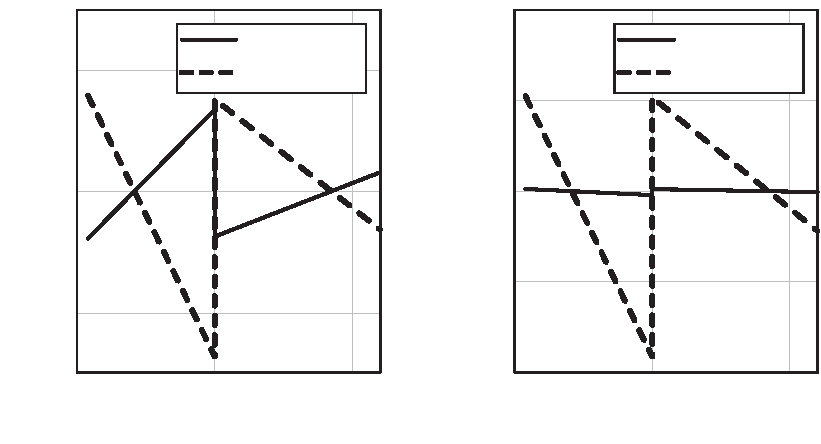
\includegraphics[width=\unitlength]{tm_stress_si_compos_2fig_bf33_lk5.pdf}}%
        \put(0.08193627,0.04661595){\color[named]{black}\makebox(0,0)[lb]{\smash{$-$0.5}}}%
        \put(0.26197873,0.04661588){\color[named]{black}\makebox(0,0)[lb]{\smash{0}}}%
        \put(0.41837149,0.04661588){\color[named]{black}\makebox(0,0)[lb]{\smash{0.5}}}%
        \put(0.08422509,0.14380795){\color[named]{black}\makebox(0,0)[rb]{\smash{$-$20}}}%
        \put(0.08422509,0.2925718){\color[named]{black}\makebox(0,0)[rb]{\smash{0}}}%
        \put(0.08422509,0.43950478){\color[named]{black}\makebox(0,0)[rb]{\smash{20}}}%
        \put(0.3001233,0.48146381){\color[named]{black}\makebox(0,0)[lb]{\smash{\small{Истин.}}}}%
        \put(0.3001233,0.44133571){\color[named]{black}\makebox(0,0)[lb]{\smash{{\small Средний}}}}%
        \put(0.27917176,0.012){\color[named]{black}\makebox(0,0)[b]{\smash{$z$, мм}}}%
        \put(0.02471946,0.30516171){\color[named]{black}\rotatebox{90}{\makebox(0,0)[b]{\smash{$\sigma_x^T$, МПа}}}}%
        \put(0.61596035,0.04661595){\color[named]{black}\makebox(0,0)[lb]{\smash{$-$0.5}}}%
        \put(0.79600281,0.04661588){\color[named]{black}\makebox(0,0)[lb]{\smash{0}}}%
        \put(0.95239558,0.04661588){\color[named]{black}\makebox(0,0)[lb]{\smash{0.5}}}%
        \put(0.61824917,0.18195252){\color[named]{black}\makebox(0,0)[rb]{\smash{$-$20}}}%
        \put(0.61824917,0.2925718){\color[named]{black}\makebox(0,0)[rb]{\smash{0}}}%
        \put(0.61824917,0.40319107){\color[named]{black}\makebox(0,0)[rb]{\smash{20}}}%
        \put(0.61824917,0.51381035){\color[named]{black}\makebox(0,0)[rb]{\smash{40}}}%
        \put(0.83414739,0.48146381){\color[named]{black}\makebox(0,0)[lb]{\small{Истин.}}}%
        \put(0.83414739,0.44133571){\color[named]{black}\makebox(0,0)[lb]{\small{Средний}}}%
        \put(0.81319588,0.012){\color[named]{black}\makebox(0,0)[b]{\smash{$z$, мм}}}%
        \put(0.55874372,0.30516171){\color[named]{black}\rotatebox{90}{\makebox(0,0)[b]{\smash{$\sigma_x^T$, МПа}}}}%
        \put(0.61824917,0.07209782){\color[named]{black}\makebox(0,0)[rb]{\smash{$-$40}}}%
        \put(0.098,-0.04){%
        \fcolorbox{black}{siliconcolour}{\makebox[0.108\textwidth]{Si}}%
        \fcolorbox{black}{glasscolour}{\makebox[0.147\textwidth]{Borofloat 33}}%
        }%
        \put(0.63,-0.04){%
        \fcolorbox{black}{siliconcolour}{\makebox[0.110\textwidth]{Si}}%
        \fcolorbox{black}{glasscolour}{\rule[1pt]{0pt}{6pt}\makebox[0.140\textwidth]{ЛК5}}%
        }%
      \end{picture}%
    \endgroup%

    \caption{Расчётная оценка остаточных напряжений в~кремнии для двух стёкол (модель многослойного композиционного материала для истинных и~средних ТКЛР)
    при $T_w$ = 20~{\textdegree}C, $T_b$ = 400~{\textdegree}C}
    \label{fig:tm_stress_si_compos_2fig_bf33_lk5}
\end{figure}

На Рисунке~\ref{fig:tm_stress_si_compos_2fig_bf33_lk5} графиками
показана расчётная оценка по модели многослойного композиционного
материала остаточных напряжений по~толщине сборки при температуре
20~{\textdegree}C в зависимости от температуры соединения с~разными
марками стекла. Видно, что результаты заметно отличаются.

\setlength\intextsep{0ex}%
\begin{wraptable}[19]{O}{0.50\textwidth}
  	\caption{Расчётные вариации остаточных напряжений для различных марок стёкол}%
  	\label{tab_sigma_var}% label всегда желательно идти после caption
  	\def\tabularxcolumn#1{m{#1}}
   	\begin{tabularx}{\linewidth}{@{}
   	>{\raggedright}X
   	c
   	c
   	}
    \toprule     %%% верхняя линейка
    {Марка стекла} &
    {$\sigma_w$}%, МПа
    &
    {$\sigma_b$}%, МПа
    \\
    \midrule%%% тонкий разделитель
    ЛК5 &
    7,5 &
    3,8\\
    Corning 7740 &
    6,5 &
    4,9\\
    Schott Borofloat 33 &
    5,1 &
    8,7\\
    Hoya SD\nobreakdash-2 &
    3,5 &
    0,3\\
    Asahi SW\nobreakdash-YY &
    2,2 &
    0,4\\
    \midrule%%% тонкий разделитель
    \multicolumn{3}{@{}p{\linewidth}}{
        Примечание "---
        расчётные разбросы (вариации) остаточных напряжений
        по модели двух тонких слоёв, МПа:
        $\sigma_w=|\sigma_{si}^{-60} - \sigma_{si}^{85}|$ "--- в рабочем диапазоне температур;
        $\sigma_b=|\sigma_{si}^{250} - \sigma_{si}^{450}|$ "--- в диапазоне допустимых температур соединения.
    }
    \\
    \bottomrule %%% нижняя линейка
   	\end{tabularx}%
\end{wraptable}

Из расчёта, проиллюстрированного Рисунками~\ref{fig:nakop_deform}~и~\ref{fig:nakop_deform_xtb},
видно, что между разными марками стекла есть различие как в разбросе
(вариации) остаточных напряжений в зависимости от рабочей температуры,
так и в разбросе (вариации) остаточных напряжений в зависимости от~температуры соединения.

В Таблицу~\ref{tab_sigma_var} сведены рассчитанные по модели двух
тонких слоёв разбросы для пяти марок стёкол, применяемых при
проведении анодной посадки в разных странах мира. Для расчёта
использованы толщина кремния 460~мкм, стекла "--- 600~мкм.

Значения разброса напряжений, связанного с изменением температуры
соединения,  $\sigma_b$, показывают степень влияния изменения
температуры соединения кремния с~данными марками стёкол на получаемые
напряжения.

Существует такая толщина стекла ${h_g}= H_0 \cdot h_{si}$, при которой
напряжения на~поверхности кремния будут минимальными во~всём рабочем диапазоне температур.
Эта же толщина будет толщиной смены знака напряжений.
Она связана с~параметрами жёсткости стекла (Таблица~\ref{tab_h0_stekla}).

\begingroup
В случае учёта температурной зависимости модуля Юнга материалов в расчётах,
для
определения оптимальной толщины нужно рассматривать каждую конкретную
комбинацию стекла и~кремния с~учётом всех допустимых диапазонов
температур соединения и~их~влияния на~напряжения в~рабочем диапазоне.
При~этом может быть найден узкий диапазон соотношений толщин стекла
и~кремния, удовлетворяющий целям оптимизации.\russianpar
\endgroup

\setlength\intextsep{0em}%
\begin{wraptable}[12]{O}{0.50\textwidth}
	\caption{Расчётное значение оптимального отношения толщины
	стекла к~толщине кремния
	(для неструктурированных материалов)}%
    \label{tab_h0_stekla}
    \begin{tabularx}{\linewidth}{@{}Xrrr@{}}
        \toprule     %%% верхняя линейка
        Марка стекла & $E$, ГПа &  $ \nu $ & $ H_0 $ \\
        \midrule %%% тонкий разделитель
        Corning 7740 & 62,75 & 0,200 & 3,12 \\
        Borofloat~33 & 64,00 & 0,200 & 3,09\\
        ЛК5 & 68,45 & 0,184 & 3,05\\
        Asahi SW-YY & 82,00 & 0,200 & 2,76\\
        Hoya SD-2 & 86,89 & 0,244 & 2,54\\
        \bottomrule %%% нижняя линейка
    \end{tabularx}
\end{wraptable}

В случае структурированных поверхностей, например мембранных структур,
имеет место несплошной контакт соединяемых кремния и стекла. Для таких
случаев применяется моделирование конечными элементами.
Описанные ранее модели позволяют облегчить подготовительные шаги
и~область поиска для задания граничных условий.

\setlength\intextsep{0em}%
\begin{wrapfigure}[21]{O}{0.5\textwidth}
    \ifdefmacro{\tikzsetnextfilename}{\tikzsetnextfilename{syn_a5_ThirdInvStress}}{}%
    % Created by tikzDevice version 0.10.1 on 2016-06-05 17:57:19
% !TEX encoding = UTF-8 Unicode
\begin{tikzpicture}[x=1pt,y=1pt]
\definecolor{white}{RGB}{255,255,255}
\definecolor{gray98}{gray}{0.98}
\definecolor{gray90}{gray}{0.90}
\definecolor{black}{RGB}{0,0,0}
\path[use as bounding box,fill=white] (0,0) rectangle (165.03,165.03);
\begin{scope}
\path[clip] (  0.00,  0.00) rectangle (165.03,165.03);

\path[draw=white,line width= 0.6pt,line join=round,line cap=round,fill=white] ( -0.00,  0.00) rectangle (165.03,165.03);
\end{scope}
\begin{scope}
\path[clip] ( 28.48, 25.69) rectangle (162.01,144.45);

\path[fill=white] ( 28.48, 25.69) rectangle (162.01,144.45);

\path[draw=gray98,line width= 0.6pt,line join=round] ( 28.48, 44.09) --
	(162.01, 44.09);

\path[draw=gray98,line width= 0.6pt,line join=round] ( 28.48, 82.22) --
	(162.01, 82.22);

\path[draw=gray98,line width= 0.6pt,line join=round] ( 28.48,120.34) --
	(162.01,120.34);

\path[draw=gray98,line width= 0.6pt,line join=round] ( 45.39, 25.69) --
	( 45.39,144.45);

\path[draw=gray98,line width= 0.6pt,line join=round] ( 71.41, 25.69) --
	( 71.41,144.45);

\path[draw=gray98,line width= 0.6pt,line join=round] ( 99.59, 25.69) --
	( 99.59,144.45);

\path[draw=gray98,line width= 0.6pt,line join=round] (123.43, 25.69) --
	(123.43,144.45);

\path[draw=gray98,line width= 0.6pt,line join=round] (145.11, 25.69) --
	(145.11,144.45);

\path[draw=gray90,line width= 0.2pt,line join=round] ( 28.48, 63.15) --
	(162.01, 63.15);

\path[draw=gray90,line width= 0.2pt,line join=round] ( 28.48,101.28) --
	(162.01,101.28);

\path[draw=gray90,line width= 0.2pt,line join=round] ( 28.48,139.40) --
	(162.01,139.40);

\path[draw=gray90,line width= 0.2pt,line join=round] ( 34.55, 25.69) --
	( 34.55,144.45);

\path[draw=gray90,line width= 0.2pt,line join=round] ( 56.23, 25.69) --
	( 56.23,144.45);

\path[draw=gray90,line width= 0.2pt,line join=round] ( 86.58, 25.69) --
	( 86.58,144.45);

\path[draw=gray90,line width= 0.2pt,line join=round] (112.59, 25.69) --
	(112.59,144.45);

\path[draw=gray90,line width= 0.2pt,line join=round] (134.27, 25.69) --
	(134.27,144.45);

\path[draw=gray90,line width= 0.2pt,line join=round] (155.95, 25.69) --
	(155.95,144.45);

\path[draw=black,line width= 1.4pt,dash pattern=on 4pt off 4pt ,line join=round] ( 34.55, 31.08) --
	( 45.83, 43.75) --
	( 47.56, 47.28) --
	( 51.90, 56.75) --
	( 56.23, 64.34) --
	( 58.40, 69.42) --
	( 73.57, 95.67) --
	( 77.91,101.32) --
	( 82.24,106.30) --
	( 86.58,110.69) --
	( 90.91,114.55) --
	(112.59,127.94) --
	(155.95,139.05);

\path[draw=black,line width= 1.4pt,line join=round] ( 34.55, 52.54) --
	( 45.83, 56.73) --
	( 47.56, 57.90) --
	( 51.90, 61.04) --
	( 56.23, 63.56) --
	( 58.40, 65.24) --
	( 73.57, 73.93) --
	( 77.91, 75.80) --
	( 82.24, 77.45) --
	( 86.58, 78.91) --
	( 90.91, 80.19) --
	(112.59, 84.62) --
	(155.95, 88.30);

\path[draw=black,line width= 1.4pt,dash pattern=on 1pt off 3pt on 4pt off 3pt ,line join=round] ( 34.55, 62.60) --
	( 45.83, 62.82) --
	( 47.56, 62.88) --
	( 51.90, 63.04) --
	( 56.23, 63.18) --
	( 58.40, 63.26) --
	( 73.57, 63.72) --
	( 77.91, 63.82) --
	( 82.24, 63.91) --
	( 86.58, 63.98) --
	( 90.91, 64.05) --
	(112.59, 64.28) --
	(155.95, 64.48);

\path[draw=black,line width= 0.9pt,line join=round,line cap=round] ( 28.48, 25.69) rectangle (162.01,144.45);
\end{scope}
\begin{scope}
\path[clip] (  0.00,  0.00) rectangle (165.03,165.03);

\node[text=black,anchor=base east,inner sep=0pt, outer sep=0pt, scale=  0.90] at ( 23.08, 60.06) {0};

\node[text=black,anchor=base east,inner sep=0pt, outer sep=0pt, scale=  0.90] at ( 23.08, 98.18) {5};

\node[text=black,anchor=base east,inner sep=0pt, outer sep=0pt, scale=  0.90] at ( 23.08,136.30) {10};
\end{scope}
\begin{scope}
\path[clip] (  0.00,  0.00) rectangle (165.03,165.03);

\path[draw=black,line width= 0.6pt,line join=round] ( 25.48, 63.15) --
	( 28.48, 63.15);

\path[draw=black,line width= 0.6pt,line join=round] ( 25.48,101.28) --
	( 28.48,101.28);

\path[draw=black,line width= 0.6pt,line join=round] ( 25.48,139.40) --
	( 28.48,139.40);
\end{scope}
\begin{scope}
\path[clip] (  0.00,  0.00) rectangle (165.03,165.03);

\path[draw=black,line width= 0.6pt,line join=round] ( 34.55, 22.69) --
	( 34.55, 25.69);

\path[draw=black,line width= 0.6pt,line join=round] ( 56.23, 22.69) --
	( 56.23, 25.69);

\path[draw=black,line width= 0.6pt,line join=round] ( 86.58, 22.69) --
	( 86.58, 25.69);

\path[draw=black,line width= 0.6pt,line join=round] (112.59, 22.69) --
	(112.59, 25.69);

\path[draw=black,line width= 0.6pt,line join=round] (134.27, 22.69) --
	(134.27, 25.69);

\path[draw=black,line width= 0.6pt,line join=round] (155.95, 22.69) --
	(155.95, 25.69);
\end{scope}
\begin{scope}
\path[clip] (  0.00,  0.00) rectangle (165.03,165.03);

\node[text=black,anchor=base,inner sep=0pt, outer sep=0pt, scale=  0.90] at ( 34.55, 14.09) {200};

\node[text=black,anchor=base,inner sep=0pt, outer sep=0pt, scale=  0.90] at ( 56.23, 14.09) {700};

\node[text=black,anchor=base,inner sep=0pt, outer sep=0pt, scale=  0.90] at ( 86.58, 14.09) {1400};

\node[text=black,anchor=base,inner sep=0pt, outer sep=0pt, scale=  0.90] at (112.59, 14.09) {2000};

\node[text=black,anchor=base,inner sep=0pt, outer sep=0pt, scale=  0.90] at (134.27, 14.09) {2500};

\node[text=black,anchor=base,inner sep=0pt, outer sep=0pt, scale=  0.90] at (155.95, 14.09) {3000};
\end{scope}
\begin{scope}
\path[clip] (  0.00,  0.00) rectangle (165.03,165.03);

\node[text=black,anchor=base,inner sep=0pt, outer sep=0pt, scale=  1.00] at ( 95.25,  2.40) {Толщина стекла, мкм};
\end{scope}
\begin{scope}
\path[clip] (  0.00,  0.00) rectangle (165.03,165.03);

\node[text=black,rotate= 90.00,anchor=base,inner sep=0pt, outer sep=0pt, scale=  1.00] at (  9.29, 85.07) {Напряжение, МПа};
\end{scope}
\begin{scope}
\path[clip] (  0.00,  0.00) rectangle (165.03,165.03);

\path[draw=black,line width= 0.6pt,line join=round,line cap=round,fill=white] ( 31.16,101.02) rectangle ( 95.22,142.07);
\end{scope}
\begin{scope}
\path[clip] (  0.00,  0.00) rectangle (165.03,165.03);

\path[draw=white,line width= 0.6pt,line join=round,line cap=round,fill=white] ( 35.42,124.56) rectangle ( 59.51,134.19);
\end{scope}
\begin{scope}
\path[clip] (  0.00,  0.00) rectangle (165.03,165.03);

\path[draw=black,line width= 1.4pt,dash pattern=on 4pt off 4pt ,line join=round] ( 37.83,129.37) -- ( 57.10,129.37);
\end{scope}
\begin{scope}
\path[clip] (  0.00,  0.00) rectangle (165.03,165.03);

\path[draw=white,line width= 0.6pt,line join=round,line cap=round,fill=white] ( 35.42,114.92) rectangle ( 59.51,124.56);
\end{scope}
\begin{scope}
\path[clip] (  0.00,  0.00) rectangle (165.03,165.03);

\path[draw=black,line width= 1.4pt,line join=round] ( 37.83,119.74) -- ( 57.10,119.74);
\end{scope}
\begin{scope}
\path[clip] (  0.00,  0.00) rectangle (165.03,165.03);

\path[draw=white,line width= 0.6pt,line join=round,line cap=round,fill=white] ( 35.42,105.28) rectangle ( 59.51,114.92);
\end{scope}
\begin{scope}
\path[clip] (  0.00,  0.00) rectangle (165.03,165.03);

\path[draw=black,line width= 1.4pt,dash pattern=on 1pt off 3pt on 4pt off 3pt ,line join=round] ( 37.83,110.10) -- ( 57.10,110.10);
\end{scope}
\begin{scope}
\path[clip] (  0.00,  0.00) rectangle (165.03,165.03);

\node[text=black,anchor=base east,inner sep=0pt, outer sep=0pt, scale=  0.90] at ( 90.95,126.27) {\(-\)60 \({}^\circ\)C};
\end{scope}
\begin{scope}
\path[clip] (  0.00,  0.00) rectangle (165.03,165.03);

\node[text=black,anchor=base east,inner sep=0pt, outer sep=0pt, scale=  0.90] at ( 90.95,116.64) {20 \({}^\circ\)C};
\end{scope}
\begin{scope}
\path[clip] (  0.00,  0.00) rectangle (165.03,165.03);

\node[text=black,anchor=base east,inner sep=0pt, outer sep=0pt, scale=  0.90] at ( 90.95,107.00) {85 \({}^\circ\)C};
\end{scope}
\begin{scope}
\path[clip] (  0.00,  0.00) rectangle (165.03,165.03);

\node[text=black,anchor=base,inner sep=0pt, outer sep=0pt, scale=  1.00] at ( 95.25,157.69) {Третий инвариант тензора};

\node[text=black,anchor=base,inner sep=0pt, outer sep=0pt, scale=  1.00] at ( 95.25,146.89) {девиатора напряжений};
\end{scope}
\end{tikzpicture}
%
    \caption{Смоделированная оценка остаточных напряжений на~открытой
    поверхности кремниевой мембраны для различных толщин стекла ЛК5 при нескольких
    рабочих температурах}% Этот текст попадает в названия рисунков в списке
    % рисунков
    \label{fig:si_membrane_third_inv_stress}
\end{wrapfigure}

Моделирование методом конечных элементов
подтверждает форму эпюр расчётных напряжений
и~возможность снижения напряжений за~счёт подбора толщин материалов.
На Рисунке~\ref{fig:si_membrane_third_inv_stress} показаны результаты
моделирования конечными элементами сборки кремниевого элемента
размерами \mbox{4\(\,\times\,\)4\(\,\times\,\)0,46 мм} с~мембраной толщиной
50~мкм и~стеклянного элемента размерами \mbox{4\(\,\times\,\)4 мм} нескольких толщин.
Площадь области соединения со~стеклом составляла половину от
площади поверхности стеклянного элемента.
Температура проведения смоделированного соединения %NEEDFIX «температура проведения смоделированного соединения» = стилистическая ошибка по мнению ведущей организации, но залитый в ВАК диссер изменять нельзя, так что это не подлежит исправлению в исходниках моей диссертации
300~{\textdegree}C. Марка стекла "--- ЛК5.
Расчётная оптимальная толщина стекла для сплошного кремния такой
толщины "--- 1400~мкм.
Видно, что вычисляемая оптимальная толщина стала меньше
пропорционально площади соединения со стеклом.

В \underline{\textbf{четвёртой главе}} описаны эксперименты,
проведённые для подтверждения утверждений из~предыдущих глав. Описаны
исследования и~практический опыт по снижению остаточных напряжений
посредством термообработки. Предложена методика минимизации остаточных
напряжений, представленная в виде шагов для разработчика прибора.
Также описаны сложности, на которые стоит обратить внимание при
разработке современной электронной техники с~применением технологии
электростатического соединения.

Метод рамановской спектроскопии (РС) (в отечественной литературе
известный как спектроскопия комбинационного рассеяния (КР)
света) применяется для исследования спектров электронных возбуждений и
оптических фононов в разных веществах.
Метод РС основан на эффекте неупругого рассеяния света на возбуждениях
системы при воздействии лазерного излучения. Исследуется сдвиг частоты
отражённого лазерного излучения.

На дисперсионном Раман микроскопе Nicolet DXR Spectrometer
измеряли пластины диаметром 100~мм кремния марки КЭФ (кремний
электронного типа проводимости, легирующий элемент "--- фосфор)
односторонней (ОП) и двусторонней полировки (ДП) с~удельным
сопротивлением 4,5~Ом$\cdot$см в свободном состоянии и после
соединения с пластинами стекла марки Borofloat~33.
Для возбуждения использовался лазер с длиной волны 633~нм. Апертура
устанавливалась в 25 мкм с формой отверстия. Использовался объектив
10х/0.25 BD и решётка разрешением 1200 линий/мм.

Рамановская спектроскопия поверхности кремния качественно подтвердила
повышение величины напряжений с~повышением температуры
у~соответствующих образцов.

Метод поляризационно-оптического измерения разности хода лучей основан
на явлении двулучепреломления, которое наблюдается в напряжённом
стекле при прохождении через него луча линейно-поляризованного света,
и заключается в разложении луча на два: обыкновенный и необыкновенный,
распространяющиеся с различными скоростями и~вследствие этого имеющие
при выходе из напряжённого стекла разность хода.

Для экспериментальной проверки распределения напряжений
использовались пластины кремния марки КЭС (кремний электронного типа
проводимости, легирующий элемент "--- сурьма) диаметром 60 мм
ориентации \{100\} с~удельным сопротивлением 0,01 Ом$\cdot$см и
прямоугольные пластины стекла ЛК5 размерами 30\(\,\times\,\)50\(\,\times\,\)4,5~мм. Соединения были проведены при температуре от~330
до~350~{\textdegree}C. Измерения величины двулучепреломления в~стекле
проводились на полярископе\nb-поляриметре ПКС\nb-250.

В сборках стекло"--~кремний наблюдалась смена знака напряжений в~стекле от
растягивающих к сжимающим по мере удаления от границы соединения, что хорошо
соотносится с расчётными результатами, приведёнными
на~Рисунке~\ref{fig:tm_stress_si_compos_2fig_bf33_lk5}
на~странице~\pageref{fig:tm_stress_si_compos_2fig_bf33_lk5}.

Для исследования влияния
термообработки на остаточные напряжения
использовались кристаллы кремния
размером 4\(\,\times\,\)4~мм и толщиной 0,4~мм с вытравленной полостью. Они были
предварительно электростатически соединены с пьедесталами из стекла ЛК5 толщиной
5~мм при температуре 440~{\textdegree}C. Ширина обода контакта
кремния со стеклом составляла 0,7~мм.

Первый вариант термообработки: нагрев до температуры
(415\(\pm\)30)~{\textdegree}C, выдержка 60 минут и затем неуправляемое охлаждение.
Второй вариант "--- нагрев до температуры
(440\(\pm\)30)~{\textdegree}C, выдержка 15 минут и затем управляемое охлаждение со
скоростью не~превышающей 3~{\textdegree}C/мин. Охлаждение проводилось до
температуры 200~{\textdegree}C, на которой проходила выдержка 30~минут. Затем
образцы охлаждались в~неконтролируемом режиме.
Величина остаточных напряжений в~стекле для каждого
из~вариантов была снижена за~счёт этой термообработки более чем в~2~раза.

Проведены эксперименты по снижению остаточных напряжений
за~счёт управляемого охлаждения.
Среднеарифметическая величина остаточных напряжений в~стекле
у образцов с управляемым охлаждением составила
63~\% от~исходного значения.

Результаты экспериментов продемонстрировали возможность снижения внутренних
механических напряжений при помощи термообработки и~возможность совмещения
процессов соединения и последующего отжига. Для стекла ЛК5 возможно снижать
напряжения за счёт охлаждения со~скоростью 2~{\textdegree}C/мин.
Предположительно, этот вывод можно распространить и~на~другие боросиликатные
стёкла, совместимые с~анодной посадкой: Schott Borofloat~33 и Corning~7740.

Проведённые автором диссертационного исследования эксперименты
по проведению процесса в режиме ограничения
тока средствами импульсного источника высокого напряжения (за~счёт
плавного нарастания подводимой к пластинам разности потенциалов,
использовалось ограничение до уровня плотности тока
0,4~А/м{\textsuperscript{2}}) продемонстрировали снижение риска
возникновения прожигов стекла и локального перегрева.

На основании описанных в~третьей главе примеров применения моделей
оценки остаточных напряжений в работе предложены следующие шаги
минимизации напряжений при разработке конструкции приборов
электронной техники:

\begin{enumerate}
    \item Определить рабочий диапазон температур прибора
    и верхнюю границу температуры соединения.
    \item Получить термомеханические характеристики кремния и стекла,
    доступных к~применению.
    \item\label{shag_vybora_stekla} Выбрать марку стекла, сравнив эти
    характеристики.
    \item По модели двух тонких слоёв примерно определить температуру
    проведения процесса.
    \item При необходимости, учесть несимметричность распределения
    напряжений в рабочем диапазоне температур, соответствующим образом
    подобрав температуру соединения.
    \item Выбрать толщину стекла (с учётом поправки на площадь
    соединения), если конструкция позволяет.
    \item По возможности, провести более точное моделирование методом
    конечных элементов.
    \item При необходимости повторить шаги, начиная
    с~\ref{shag_vybora_stekla}.
\end{enumerate}

В \underline{\textbf{общих выводах и заключении}} приведены краткие выводы %NEEDFIX «в общих выводах приведены краткие выводы» = стилистическая ошибка по мнению ведущей организации, но залитый в ВАК диссер изменять нельзя, так что это не подлежит исправлению в исходниках моей диссертации
по~результатам проведённых в~работе исследований.

\providecommand{\beforevyvods}%
{В диссертации поставлена и решена
научно-техническая задача
исследования методов снижения остаточных напряжений
при~электростатическом соединении кремния со~стеклом.}

%В заключении диссертации излагаются итоги выполненного исследования, рекомендации, перспективы дальнейшей разработки темы.

\newcommand{\vyvodi}%
{%
\item \label{vyvod_one}Расчётным путём выявлено, что для электростатического соединения
с минимальными остаточными напряжениями \mmark{подбор стекла}, согласованного
с кремнием по ТКЛР, следует осуществлять \mmark{по~критерию минимальности
накапливаемой разности между ТКЛР}, в~процессе охлаждения с температуры
соединения до диапазона рабочих температур прибора.
}

\newcommand{\vyvodii}%
{\item \label{vyvod_two}Для моделирования сборок
кремния со~стёклами марок
ЛК5, Borofloat~33, 7740, SD-2
в~диапазоне температур от~минус~100 до~500~{\textdegree}C
следует \mmark{использовать
полученные} автором диссертационной работы
\mmark{температурные зависимости ТКЛР} для этого диапазона температур.}

\newcommand{\vyvodiii}%
{\item \label{vyvod_three}Показано, что
\mmark{предварительный расчёт по моделям}
двух тонких слоёв и~многослойного композиционного материала
\mmark{с учётом динамики накопления}
остаточных напряжений
\mmark{повышает
эффективность} применения
моделирования методом \mmark{конечных элементов}.
}

\newcommand{\vyvodivmain}%
{\mmark{Для минимизации} остаточных \mmark{напряжений на поверхности} сплошного кремния необходимо \mmark{выбирать толщину стекла}:%
    \begin{itemize}
        \item алюмосиликатного (SD-2, SW-YY) в~2,5"--~2,8~раза больше
        толщины кремния.
        \item боросиликатного (ЛК5, 7740, Borofloat 33) в~3~раза больше
        толщины кремния.
    \end{itemize}
}
\newcommand{\vyvodiv}%
{\item \label{vyvod_four}\vyvodivmain
    Это объясняется разницей в согласованности жёсткости стекла и~кремния.
    Остаточные напряжения на поверхности кремния минимизируются за счёт компенсации деформаций, вызванных тепловым расширением кремния, деформациями, вызванными воздействием присоединённого стекла.%
}

\newcommand{\vyvodv}%
{\item \label{vyvod_five}\mmark{При охлаждении} сборки
со~скоростью
\mmark{не более
2~{\textdegree}C/мин}
после окончания подачи высокого напряжения
\mmark{происходит снижение остаточных напряжений} в стекле
(например в~ЛК5, соединённом
с~кремнием при температуре 440~{\textdegree}C,
до 63~\% от уровня
напряжений при неконтролируемом охлаждении).
Это объясняется
релаксацией аморфной структуры стекла.%
}

\newcommand{\vyvodvi}%
{\item \label{vyvod_six}\mmark{Рекомендуется проводить} электростатическое соединение
\mmark{в~режиме ограничения тока},
что снижает риски
локального перегрева границы кремний"--~стекло
и~последующего прожига стекла.%
}

\newcommand{\vyvodsall}{\vyvodi\vyvodii\vyvodiii\vyvodiv\vyvodv\vyvodvi}

\providecommand{\aftervyvods}%
{Результаты, полученные в диссертации, могут быть использованы при разработке
и~производстве приборов электронной техники с~использованием технологии
электростатического соединения, таких как микрорезонаторы, микрореле,
микроакселерометры, микрогироскопы, чувствительные элементы датчиков
давления.
Проведённые расчёты и сделанные выводы могут способствовать импортозамещению
зарубежных марок стекла в отечественных приборах электронной техники.

\textbf{Дальнейшая разработка темы}
может состоять в разработке аналитических моделей оценки распределения
остаточных напряжений в микрообработанном кремнии,
с~использованием температурной зависимости истинных значений ТКЛР
материалов. Кроме того, востребованными будут модели, учитывающие
изменение свойств стекла, связанное с переносом ионов в~результате
проведения процесса электростатического соединения. Для этого также
потребуется дополнительное исследование свойств стёкол как по составу,
так и~по~анализу связи подвижности ионов с~температурой и~подводимой
разностью потенциалов.}

\beforevyvods

\aftervyvods

\enlargethispage*{\baselineskip}
\section{Общие выводы по работе}

\begin{enumerate}[labelindent=!, leftmargin=\parindent]
\vyvodsall
\end{enumerate}
\pagebreak

\urlstyle{rm}   % ссылки URL обычным шрифтом
\ifdefmacro{\microtypesetup}{\microtypesetup{protrusion=false}}{} % не рекомендуется применять пакет микротипографики к автоматически генерируемому списку литературы
  \insertbiblioauthorimportant  % Вывод наиболее значимых работ автора (определяется в файле characteristic во второй section)
\ifdefmacro{\microtypesetup}{\microtypesetup{protrusion=true}}{}
\urlstyle{tt}   % возвращаем установки шрифта ссылок URL
        % Содержание автореферата

\end{document}